\section{XY}
\clearpage
\subsection*{Mean request latency}
\begin{center}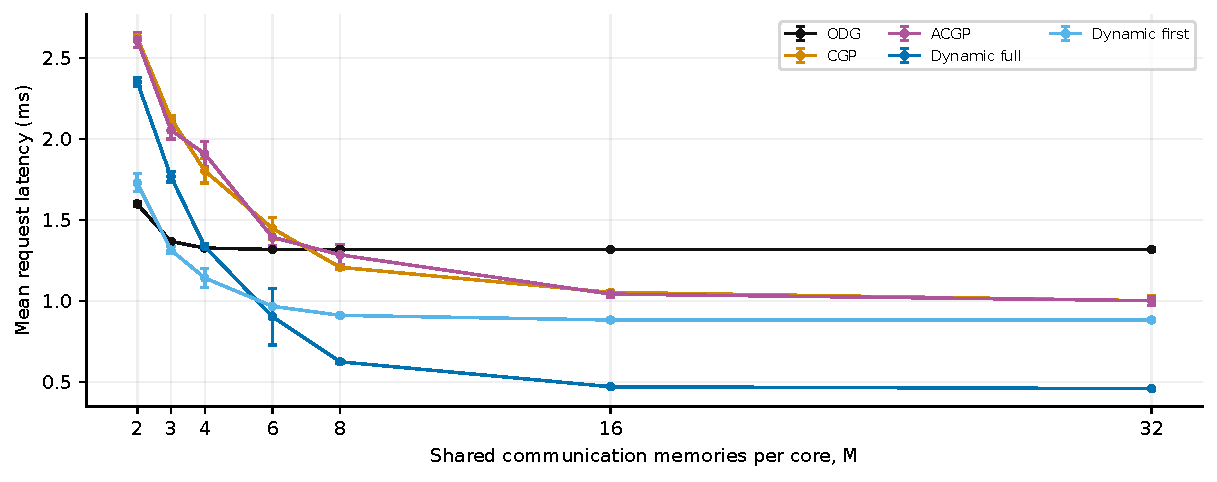
\includegraphics[width=.94\linewidth,height=.255\textheight,keepaspectratio]{figures/memory/mesh_xy_request_latency_mean_ms.pdf}\captionof{figure}{Run-level mean and sample SD. Shared trace aliases are counted once.}\end{center}
\begin{center}{\scriptsize\setlength{\tabcolsep}{3pt}
\begin{tabular}{lrrrrr}
\toprule
M & ODG & CGP & ACGP & Dynamic full & Dynamic first \\
\midrule
2 & $1.599\pm0.016$ & $2.625\pm0.000$ & $2.612\pm0.046$ & $2.353\pm0.026$ & $1.729\pm0.055$ \\
3 & $1.367\pm0.008$ & $2.126\pm0.020$ & $2.054\pm0.054$ & $1.766\pm0.032$ & $1.314\pm0.022$ \\
4 & $1.327\pm0.006$ & $1.803\pm0.075$ & $1.908\pm0.079$ & $1.335\pm0.020$ & $1.141\pm0.058$ \\
6 & $1.317\pm0.004$ & $1.448\pm0.066$ & $1.393\pm0.049$ & $0.9021\pm0.1738$ & $0.9670\pm0.0025$ \\
8 & $1.317\pm0.004$ & $1.208\pm0.015$ & $1.284\pm0.062$ & $0.6244\pm0.0106$ & $0.9111\pm0.0051$ \\
16 & $1.317\pm0.004$ & $1.053\pm0.011$ & $1.042\pm0.023$ & $0.4705\pm0.0020$ & $0.8823\pm0.0078$ \\
32 & $1.317\pm0.004$ & $1.001\pm0.032$ & $1.002\pm0.028$ & $0.4587\pm0.0006$ & $0.8823\pm0.0078$ \\
\bottomrule\end{tabular}}
\captionof{table}{Mean $\pm$ sample SD; n/a denotes a metric outside that policy's instrumentation.}
{\footnotesize\href{https://github.com/sanjeevkrishnaa/Compiler-Driven-ACE/blob/codex/ace-scheduler-correctness/docs/latex/qft96_final/data/memory_mesh_xy_request_latency_mean_ms.csv}{Exact CSV values and sample counts}}
\end{center}
\subsection*{Median request latency}
\begin{center}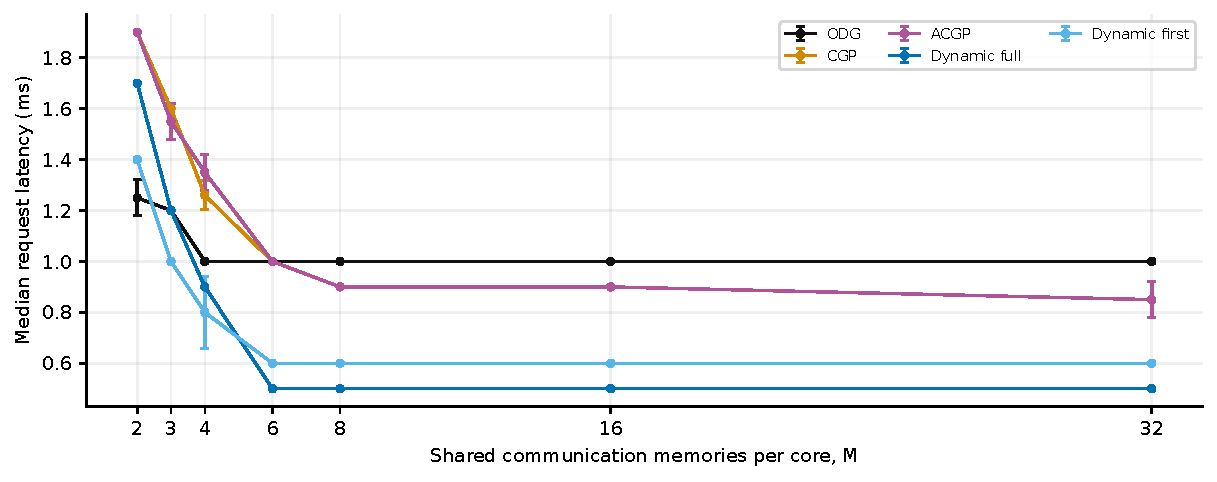
\includegraphics[width=.94\linewidth,height=.255\textheight,keepaspectratio]{figures/memory/mesh_xy_request_latency_median_ms.pdf}\captionof{figure}{Run-level mean and sample SD. Shared trace aliases are counted once.}\end{center}
\begin{center}{\scriptsize\setlength{\tabcolsep}{3pt}
\begin{tabular}{lrrrrr}
\toprule
M & ODG & CGP & ACGP & Dynamic full & Dynamic first \\
\midrule
2 & $1.250\pm0.071$ & $1.900\pm0.000$ & $1.900\pm0.000$ & $1.700\pm0.000$ & $1.400\pm0.000$ \\
3 & $1.200\pm0.000$ & $1.600\pm0.000$ & $1.550\pm0.071$ & $1.200\pm0.000$ & $1.000\pm0.000$ \\
4 & $1.000\pm0.000$ & $1.260\pm0.056$ & $1.350\pm0.071$ & $0.9000\pm0.0000$ & $0.8000\pm0.1414$ \\
6 & $1.000\pm0.000$ & $1.000\pm0.000$ & $1.000\pm0.000$ & $0.5000\pm0.0000$ & $0.6000\pm0.0000$ \\
8 & $1.000\pm0.000$ & $0.9000\pm0.0000$ & $0.9000\pm0.0000$ & $0.5000\pm0.0000$ & $0.6000\pm0.0000$ \\
16 & $1.000\pm0.000$ & $0.9000\pm0.0000$ & $0.9000\pm0.0000$ & $0.5000\pm0.0000$ & $0.6000\pm0.0000$ \\
32 & $1.000\pm0.000$ & $0.8500\pm0.0707$ & $0.8500\pm0.0707$ & $0.5000\pm0.0000$ & $0.6000\pm0.0000$ \\
\bottomrule\end{tabular}}
\captionof{table}{Mean $\pm$ sample SD; n/a denotes a metric outside that policy's instrumentation.}
{\footnotesize\href{https://github.com/sanjeevkrishnaa/Compiler-Driven-ACE/blob/codex/ace-scheduler-correctness/docs/latex/qft96_final/data/memory_mesh_xy_request_latency_median_ms.csv}{Exact CSV values and sample counts}}
\end{center}
\clearpage
\subsection*{p95 request latency}
\begin{center}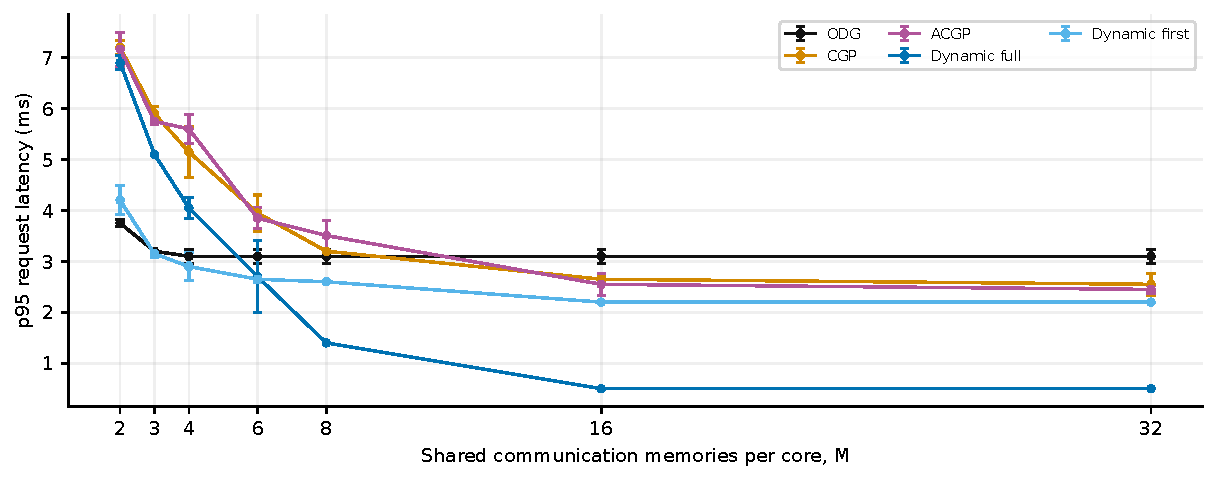
\includegraphics[width=.94\linewidth,height=.255\textheight,keepaspectratio]{figures/memory/mesh_xy_request_latency_p95_ms.pdf}\captionof{figure}{Run-level mean and sample SD. Shared trace aliases are counted once.}\end{center}
\begin{center}{\scriptsize\setlength{\tabcolsep}{3pt}
\begin{tabular}{lrrrrr}
\toprule
M & ODG & CGP & ACGP & Dynamic full & Dynamic first \\
\midrule
2 & $3.750\pm0.071$ & $7.200\pm0.141$ & $7.166\pm0.332$ & $6.900\pm0.141$ & $4.200\pm0.283$ \\
3 & $3.200\pm0.000$ & $5.900\pm0.141$ & $5.750\pm0.071$ & $5.100\pm0.000$ & $3.150\pm0.071$ \\
4 & $3.100\pm0.141$ & $5.150\pm0.495$ & $5.600\pm0.283$ & $4.050\pm0.212$ & $2.900\pm0.283$ \\
6 & $3.100\pm0.141$ & $3.950\pm0.354$ & $3.850\pm0.212$ & $2.700\pm0.707$ & $2.650\pm0.071$ \\
8 & $3.100\pm0.141$ & $3.200\pm0.000$ & $3.508\pm0.294$ & $1.400\pm0.000$ & $2.600\pm0.000$ \\
16 & $3.100\pm0.141$ & $2.650\pm0.071$ & $2.550\pm0.212$ & $0.5000\pm0.0000$ & $2.200\pm0.000$ \\
32 & $3.100\pm0.141$ & $2.550\pm0.212$ & $2.450\pm0.071$ & $0.5000\pm0.0000$ & $2.200\pm0.000$ \\
\bottomrule\end{tabular}}
\captionof{table}{Mean $\pm$ sample SD; n/a denotes a metric outside that policy's instrumentation.}
{\footnotesize\href{https://github.com/sanjeevkrishnaa/Compiler-Driven-ACE/blob/codex/ace-scheduler-correctness/docs/latex/qft96_final/data/memory_mesh_xy_request_latency_p95_ms.csv}{Exact CSV values and sample counts}}
\end{center}
\subsection*{Maximum request latency}
\begin{center}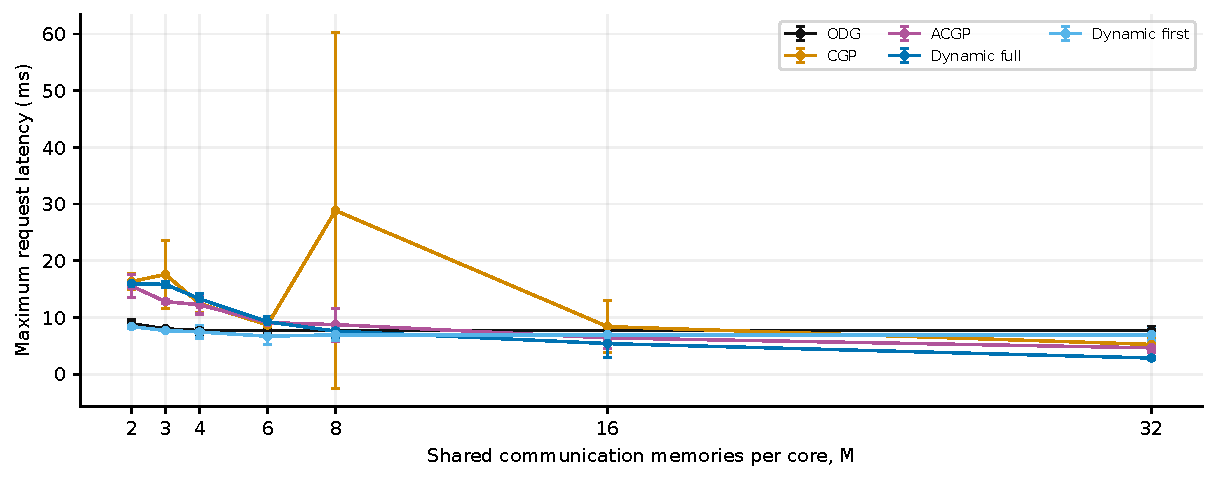
\includegraphics[width=.94\linewidth,height=.255\textheight,keepaspectratio]{figures/memory/mesh_xy_request_latency_max_ms.pdf}\captionof{figure}{Run-level mean and sample SD. Shared trace aliases are counted once.}\end{center}
\begin{center}{\scriptsize\setlength{\tabcolsep}{3pt}
\begin{tabular}{lrrrrr}
\toprule
M & ODG & CGP & ACGP & Dynamic full & Dynamic first \\
\midrule
2 & $8.900\pm0.707$ & $16.350\pm1.485$ & $15.550\pm2.051$ & $15.950\pm0.354$ & $8.400\pm0.283$ \\
3 & $8.000\pm0.283$ & $17.591\pm5.953$ & $12.800\pm0.283$ & $15.850\pm0.495$ & $7.700\pm0.000$ \\
4 & $7.700\pm0.707$ & $12.468\pm1.651$ & $12.250\pm1.626$ & $13.300\pm0.990$ & $7.450\pm1.061$ \\
6 & $7.700\pm0.707$ & $8.700\pm0.990$ & $9.100\pm0.283$ & $9.250\pm0.919$ & $6.700\pm1.414$ \\
8 & $7.700\pm0.707$ & $28.871\pm31.437$ & $8.750\pm2.899$ & $7.600\pm1.273$ & $6.950\pm1.061$ \\
16 & $7.700\pm0.707$ & $8.400\pm4.526$ & $6.400\pm1.839$ & $5.400\pm2.404$ & $6.950\pm1.061$ \\
32 & $7.700\pm0.707$ & $5.250\pm1.061$ & $4.650\pm0.778$ & $2.850\pm0.212$ & $6.950\pm1.061$ \\
\bottomrule\end{tabular}}
\captionof{table}{Mean $\pm$ sample SD; n/a denotes a metric outside that policy's instrumentation.}
{\footnotesize\href{https://github.com/sanjeevkrishnaa/Compiler-Driven-ACE/blob/codex/ace-scheduler-correctness/docs/latex/qft96_final/data/memory_mesh_xy_request_latency_max_ms.csv}{Exact CSV values and sample counts}}
\end{center}
\clearpage
\subsection*{Communication makespan}
\begin{center}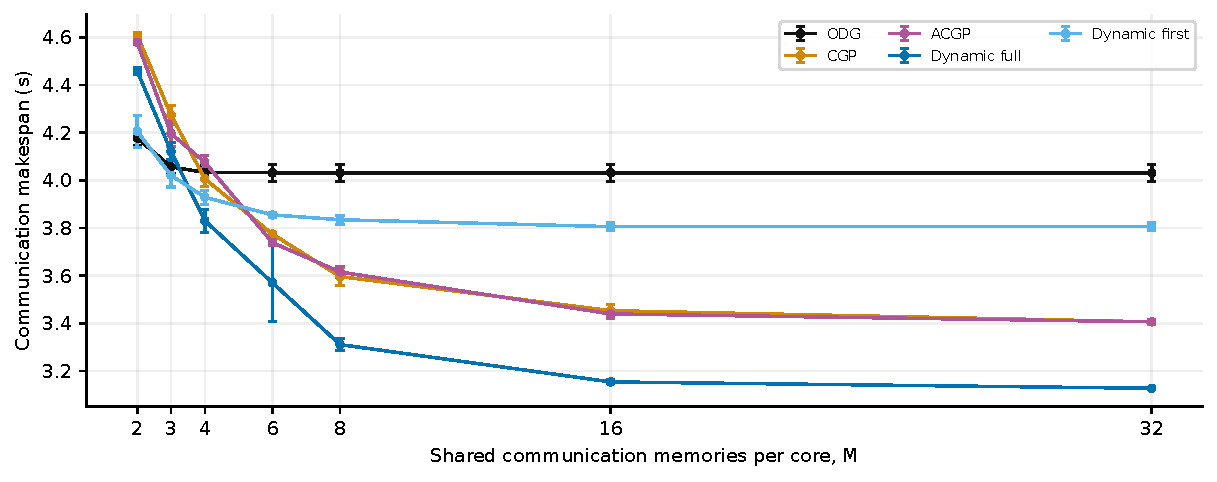
\includegraphics[width=.94\linewidth,height=.255\textheight,keepaspectratio]{figures/memory/mesh_xy_end_to_end_latency_ms.pdf}\captionof{figure}{Run-level mean and sample SD. Shared trace aliases are counted once.}\end{center}
\begin{center}{\scriptsize\setlength{\tabcolsep}{3pt}
\begin{tabular}{lrrrrr}
\toprule
M & ODG & CGP & ACGP & Dynamic full & Dynamic first \\
\midrule
2 & $4.177\pm0.031$ & $4.608\pm0.012$ & $4.578\pm0.008$ & $4.458\pm0.014$ & $4.205\pm0.067$ \\
3 & $4.056\pm0.026$ & $4.273\pm0.041$ & $4.196\pm0.054$ & $4.121\pm0.036$ & $4.021\pm0.049$ \\
4 & $4.033\pm0.031$ & $4.006\pm0.031$ & $4.075\pm0.028$ & $3.830\pm0.048$ & $3.928\pm0.029$ \\
6 & $4.031\pm0.036$ & $3.774\pm0.004$ & $3.738\pm0.013$ & $3.570\pm0.163$ & $3.854\pm0.009$ \\
8 & $4.031\pm0.036$ & $3.596\pm0.039$ & $3.615\pm0.022$ & $3.311\pm0.024$ & $3.834\pm0.019$ \\
16 & $4.031\pm0.036$ & $3.453\pm0.024$ & $3.439\pm0.018$ & $3.154\pm0.008$ & $3.805\pm0.015$ \\
32 & $4.031\pm0.036$ & $3.406\pm0.009$ & $3.406\pm0.008$ & $3.127\pm0.002$ & $3.805\pm0.015$ \\
\bottomrule\end{tabular}}
\captionof{table}{Mean $\pm$ sample SD; n/a denotes a metric outside that policy's instrumentation.}
{\footnotesize\href{https://github.com/sanjeevkrishnaa/Compiler-Driven-ACE/blob/codex/ace-scheduler-correctness/docs/latex/qft96_final/data/memory_mesh_xy_end_to_end_latency_ms.csv}{Exact CSV values and sample counts}}
\end{center}
\subsection*{Mean admission wait}
\begin{center}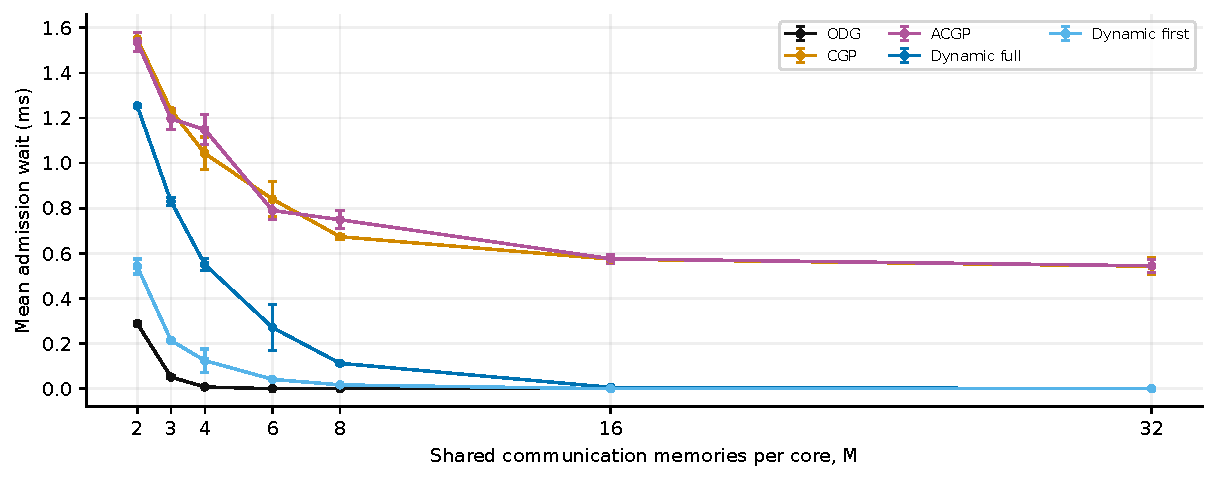
\includegraphics[width=.94\linewidth,height=.255\textheight,keepaspectratio]{figures/memory/mesh_xy_average_admission_wait_ms.pdf}\captionof{figure}{Run-level mean and sample SD. Shared trace aliases are counted once.}\end{center}
\begin{center}{\scriptsize\setlength{\tabcolsep}{3pt}
\begin{tabular}{lrrrrr}
\toprule
M & ODG & CGP & ACGP & Dynamic full & Dynamic first \\
\midrule
2 & $0.2891\pm0.0096$ & $1.550\pm0.004$ & $1.538\pm0.041$ & $1.254\pm0.005$ & $0.5419\pm0.0332$ \\
3 & $0.0517\pm0.0057$ & $1.234\pm0.003$ & $1.197\pm0.045$ & $0.8302\pm0.0184$ & $0.2138\pm0.0034$ \\
4 & $0.0080\pm0.0022$ & $1.043\pm0.073$ & $1.149\pm0.067$ & $0.5507\pm0.0249$ & $0.1248\pm0.0514$ \\
6 & $0.0000\pm0.0000$ & $0.8403\pm0.0779$ & $0.7902\pm0.0415$ & $0.2715\pm0.1027$ & $0.0418\pm0.0052$ \\
8 & $0.0000\pm0.0000$ & $0.6739\pm0.0106$ & $0.7492\pm0.0396$ & $0.1128\pm0.0036$ & $0.0171\pm0.0013$ \\
16 & $0.0000\pm0.0000$ & $0.5746\pm0.0055$ & $0.5761\pm0.0197$ & $0.0062\pm0.0002$ & $0.0000\pm0.0000$ \\
32 & $0.0000\pm0.0000$ & $0.5431\pm0.0371$ & $0.5449\pm0.0279$ & $0.0000\pm0.0000$ & $0.0000\pm0.0000$ \\
\bottomrule\end{tabular}}
\captionof{table}{Mean $\pm$ sample SD; n/a denotes a metric outside that policy's instrumentation.}
{\footnotesize\href{https://github.com/sanjeevkrishnaa/Compiler-Driven-ACE/blob/codex/ace-scheduler-correctness/docs/latex/qft96_final/data/memory_mesh_xy_average_admission_wait_ms.csv}{Exact CSV values and sample counts}}
\end{center}
\clearpage
\subsection*{Delivered EPR fidelity}
\begin{center}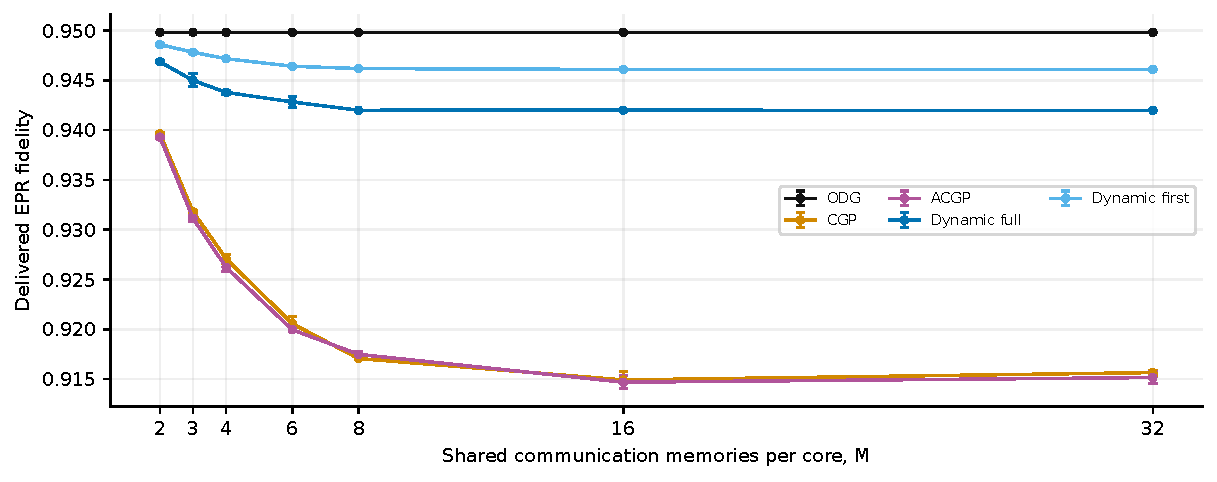
\includegraphics[width=.94\linewidth,height=.255\textheight,keepaspectratio]{figures/memory/mesh_xy_average_delivered_epr_fidelity.pdf}\captionof{figure}{Run-level mean and sample SD. Shared trace aliases are counted once.}\end{center}
\begin{center}{\scriptsize\setlength{\tabcolsep}{3pt}
\begin{tabular}{lrrrrr}
\toprule
M & ODG & CGP & ACGP & Dynamic full & Dynamic first \\
\midrule
2 & $0.9498\pm0.0000$ & $0.9396\pm0.0002$ & $0.9393\pm0.0002$ & $0.9469\pm0.0001$ & $0.9486\pm0.0001$ \\
3 & $0.9498\pm0.0000$ & $0.9318\pm0.0001$ & $0.9311\pm0.0003$ & $0.9450\pm0.0007$ & $0.9478\pm0.0001$ \\
4 & $0.9498\pm0.0000$ & $0.9271\pm0.0004$ & $0.9262\pm0.0004$ & $0.9438\pm0.0002$ & $0.9472\pm0.0000$ \\
6 & $0.9498\pm0.0000$ & $0.9206\pm0.0007$ & $0.9200\pm0.0001$ & $0.9428\pm0.0006$ & $0.9464\pm0.0000$ \\
8 & $0.9498\pm0.0000$ & $0.9171\pm0.0001$ & $0.9175\pm0.0003$ & $0.9420\pm0.0000$ & $0.9462\pm0.0000$ \\
16 & $0.9498\pm0.0000$ & $0.9149\pm0.0009$ & $0.9147\pm0.0007$ & $0.9420\pm0.0000$ & $0.9461\pm0.0000$ \\
32 & $0.9498\pm0.0000$ & $0.9157\pm0.0002$ & $0.9152\pm0.0006$ & $0.9420\pm0.0000$ & $0.9461\pm0.0000$ \\
\bottomrule\end{tabular}}
\captionof{table}{Mean $\pm$ sample SD; n/a denotes a metric outside that policy's instrumentation.}
{\footnotesize\href{https://github.com/sanjeevkrishnaa/Compiler-Driven-ACE/blob/codex/ace-scheduler-correctness/docs/latex/qft96_final/data/memory_mesh_xy_average_delivered_epr_fidelity.csv}{Exact CSV values and sample counts}}
\end{center}
\subsection*{Compiler readiness fraction}
\begin{center}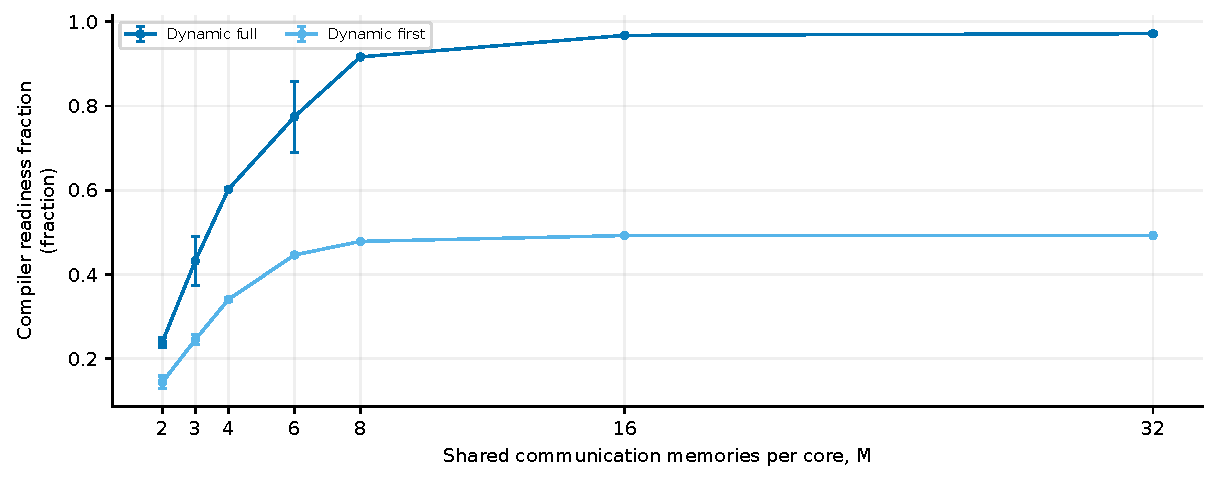
\includegraphics[width=.94\linewidth,height=.255\textheight,keepaspectratio]{figures/memory/mesh_xy_pregenerated_success_rate.pdf}\captionof{figure}{Run-level mean and sample SD. Shared trace aliases are counted once.}\end{center}
\begin{center}{\scriptsize\setlength{\tabcolsep}{3pt}
\begin{tabular}{lrrrrr}
\toprule
M & ODG & CGP & ACGP & Dynamic full & Dynamic first \\
\midrule
2 & n/a & n/a & n/a & $0.2390\pm0.0111$ & $0.1438\pm0.0151$ \\
3 & n/a & n/a & n/a & $0.4321\pm0.0580$ & $0.2451\pm0.0120$ \\
4 & n/a & n/a & n/a & $0.6017\pm0.0007$ & $0.3403\pm0.0044$ \\
6 & n/a & n/a & n/a & $0.7740\pm0.0836$ & $0.4462\pm0.0042$ \\
8 & n/a & n/a & n/a & $0.9163\pm0.0013$ & $0.4785\pm0.0005$ \\
16 & n/a & n/a & n/a & $0.9675\pm0.0004$ & $0.4924\pm0.0009$ \\
32 & n/a & n/a & n/a & $0.9715\pm0.0020$ & $0.4924\pm0.0009$ \\
\bottomrule\end{tabular}}
\captionof{table}{Mean $\pm$ sample SD; n/a denotes a metric outside that policy's instrumentation.}
{\footnotesize\href{https://github.com/sanjeevkrishnaa/Compiler-Driven-ACE/blob/codex/ace-scheduler-correctness/docs/latex/qft96_final/data/memory_mesh_xy_pregenerated_success_rate.csv}{Exact CSV values and sample counts}}
\end{center}
\clearpage
\subsection*{Intended compiler-hit fraction}
\begin{center}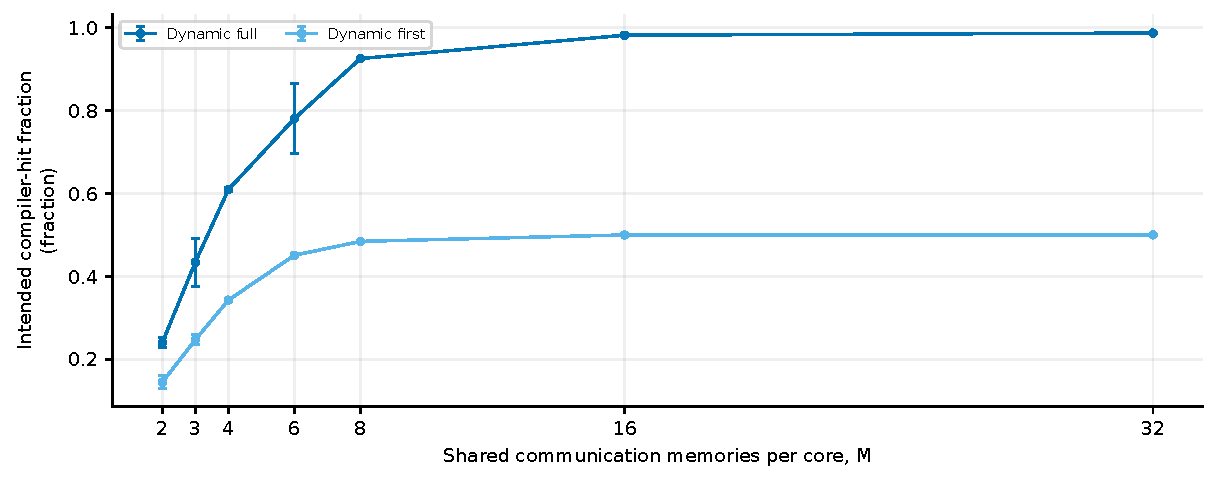
\includegraphics[width=.94\linewidth,height=.255\textheight,keepaspectratio]{figures/memory/mesh_xy_intended_request_hit_rate.pdf}\captionof{figure}{Run-level mean and sample SD. Shared trace aliases are counted once.}\end{center}
\begin{center}{\scriptsize\setlength{\tabcolsep}{3pt}
\begin{tabular}{lrrrrr}
\toprule
M & ODG & CGP & ACGP & Dynamic full & Dynamic first \\
\midrule
2 & n/a & n/a & n/a & $0.2402\pm0.0120$ & $0.1446\pm0.0155$ \\
3 & n/a & n/a & n/a & $0.4342\pm0.0584$ & $0.2472\pm0.0120$ \\
4 & n/a & n/a & n/a & $0.6094\pm0.0044$ & $0.3429\pm0.0033$ \\
6 & n/a & n/a & n/a & $0.7808\pm0.0848$ & $0.4511\pm0.0038$ \\
8 & n/a & n/a & n/a & $0.9258\pm0.0016$ & $0.4846\pm0.0002$ \\
16 & n/a & n/a & n/a & $0.9822\pm0.0033$ & $0.5003\pm0.0004$ \\
32 & n/a & n/a & n/a & $0.9875\pm0.0016$ & $0.5003\pm0.0004$ \\
\bottomrule\end{tabular}}
\captionof{table}{Mean $\pm$ sample SD; n/a denotes a metric outside that policy's instrumentation.}
{\footnotesize\href{https://github.com/sanjeevkrishnaa/Compiler-Driven-ACE/blob/codex/ace-scheduler-correctness/docs/latex/qft96_final/data/memory_mesh_xy_intended_request_hit_rate.csv}{Exact CSV values and sample counts}}
\end{center}
\subsection*{Compiler fallback fraction}
\begin{center}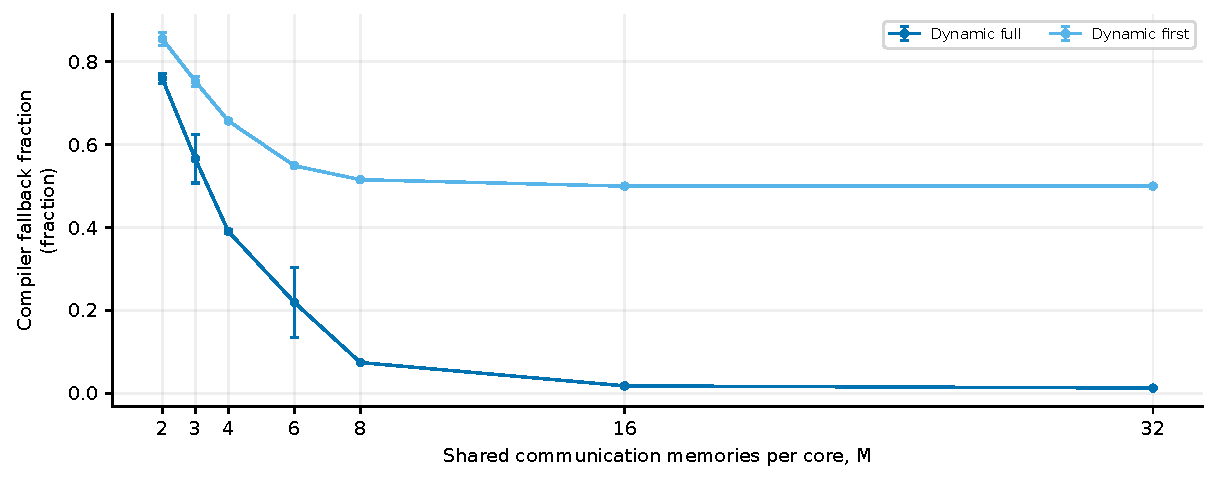
\includegraphics[width=.94\linewidth,height=.255\textheight,keepaspectratio]{figures/memory/mesh_xy_on_demand_fallback_rate.pdf}\captionof{figure}{Run-level mean and sample SD. Shared trace aliases are counted once.}\end{center}
\begin{center}{\scriptsize\setlength{\tabcolsep}{3pt}
\begin{tabular}{lrrrrr}
\toprule
M & ODG & CGP & ACGP & Dynamic full & Dynamic first \\
\midrule
2 & n/a & n/a & n/a & $0.7598\pm0.0120$ & $0.8554\pm0.0155$ \\
3 & n/a & n/a & n/a & $0.5658\pm0.0584$ & $0.7528\pm0.0120$ \\
4 & n/a & n/a & n/a & $0.3906\pm0.0044$ & $0.6571\pm0.0033$ \\
6 & n/a & n/a & n/a & $0.2192\pm0.0848$ & $0.5489\pm0.0038$ \\
8 & n/a & n/a & n/a & $0.0742\pm0.0016$ & $0.5154\pm0.0002$ \\
16 & n/a & n/a & n/a & $0.0178\pm0.0033$ & $0.4997\pm0.0004$ \\
32 & n/a & n/a & n/a & $0.0125\pm0.0016$ & $0.4997\pm0.0004$ \\
\bottomrule\end{tabular}}
\captionof{table}{Mean $\pm$ sample SD; n/a denotes a metric outside that policy's instrumentation.}
{\footnotesize\href{https://github.com/sanjeevkrishnaa/Compiler-Driven-ACE/blob/codex/ace-scheduler-correctness/docs/latex/qft96_final/data/memory_mesh_xy_on_demand_fallback_rate.csv}{Exact CSV values and sample counts}}
\end{center}
\clearpage
\subsection*{Compiler-cache waste}
\begin{center}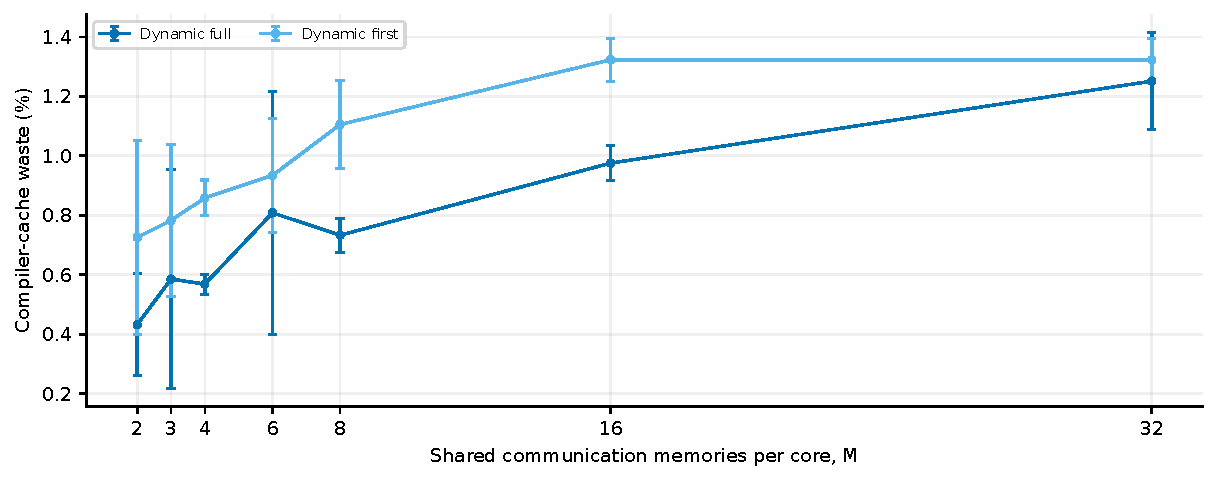
\includegraphics[width=.94\linewidth,height=.255\textheight,keepaspectratio]{figures/memory/mesh_xy_compiler_waste_percentage.pdf}\captionof{figure}{Run-level mean and sample SD. Shared trace aliases are counted once.}\end{center}
\begin{center}{\scriptsize\setlength{\tabcolsep}{3pt}
\begin{tabular}{lrrrrr}
\toprule
M & ODG & CGP & ACGP & Dynamic full & Dynamic first \\
\midrule
2 & n/a & n/a & n/a & $0.4320\pm0.1722$ & $0.7255\pm0.3260$ \\
3 & n/a & n/a & n/a & $0.5854\pm0.3690$ & $0.7827\pm0.2558$ \\
4 & n/a & n/a & n/a & $0.5684\pm0.0337$ & $0.8582\pm0.0604$ \\
6 & n/a & n/a & n/a & $0.8081\pm0.4090$ & $0.9339\pm0.1906$ \\
8 & n/a & n/a & n/a & $0.7330\pm0.0570$ & $1.105\pm0.147$ \\
16 & n/a & n/a & n/a & $0.9755\pm0.0579$ & $1.323\pm0.072$ \\
32 & n/a & n/a & n/a & $1.251\pm0.164$ & $1.323\pm0.072$ \\
\bottomrule\end{tabular}}
\captionof{table}{Mean $\pm$ sample SD; n/a denotes a metric outside that policy's instrumentation.}
{\footnotesize\href{https://github.com/sanjeevkrishnaa/Compiler-Driven-ACE/blob/codex/ace-scheduler-correctness/docs/latex/qft96_final/data/memory_mesh_xy_compiler_waste_percentage.csv}{Exact CSV values and sample counts}}
\end{center}
\subsection*{Native-protocol waste}
\begin{center}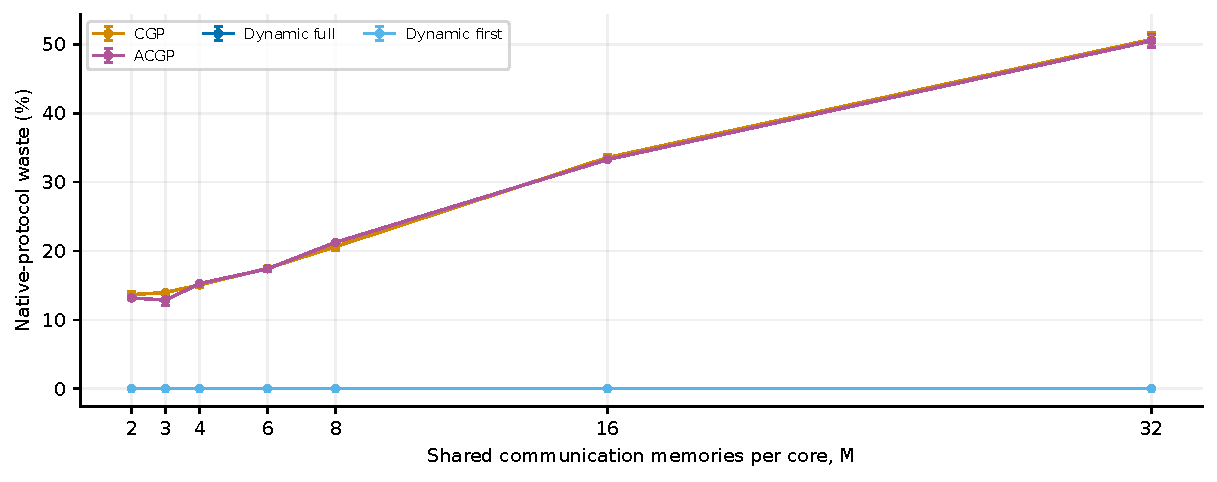
\includegraphics[width=.94\linewidth,height=.255\textheight,keepaspectratio]{figures/memory/mesh_xy_protocol_waste_percentage.pdf}\captionof{figure}{Run-level mean and sample SD. Shared trace aliases are counted once.}\end{center}
\begin{center}{\scriptsize\setlength{\tabcolsep}{3pt}
\begin{tabular}{lrrrrr}
\toprule
M & ODG & CGP & ACGP & Dynamic full & Dynamic first \\
\midrule
2 & n/a & $13.658\pm0.398$ & $13.185\pm0.195$ & $0.0000\pm0.0000$ & $0.0000\pm0.0000$ \\
3 & n/a & $13.974\pm0.073$ & $12.865\pm0.778$ & $0.0000\pm0.0000$ & $0.0000\pm0.0000$ \\
4 & n/a & $15.065\pm0.392$ & $15.269\pm0.209$ & $0.0000\pm0.0000$ & $0.0000\pm0.0000$ \\
6 & n/a & $17.490\pm0.122$ & $17.405\pm0.394$ & $0.0000\pm0.0000$ & $0.0000\pm0.0000$ \\
8 & n/a & $20.622\pm0.599$ & $21.252\pm0.082$ & $0.0000\pm0.0000$ & $0.0000\pm0.0000$ \\
16 & n/a & $33.559\pm0.465$ & $33.265\pm0.024$ & $0.0000\pm0.0000$ & $0.0000\pm0.0000$ \\
32 & n/a & $50.705\pm1.032$ & $50.498\pm0.959$ & $0.0000\pm0.0000$ & $0.0000\pm0.0000$ \\
\bottomrule\end{tabular}}
\captionof{table}{Mean $\pm$ sample SD; n/a denotes a metric outside that policy's instrumentation.}
{\footnotesize\href{https://github.com/sanjeevkrishnaa/Compiler-Driven-ACE/blob/codex/ace-scheduler-correctness/docs/latex/qft96_final/data/memory_mesh_xy_protocol_waste_percentage.csv}{Exact CSV values and sample counts}}
\end{center}
\clearpage
\subsection*{Compiler-pair expiry}
\begin{center}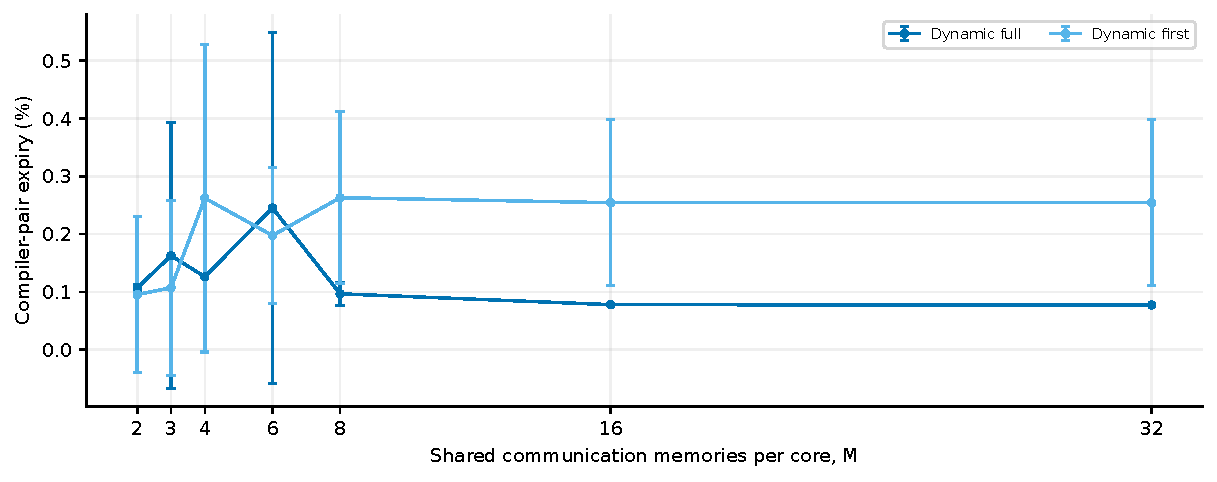
\includegraphics[width=.94\linewidth,height=.255\textheight,keepaspectratio]{figures/memory/mesh_xy_compiler_expiry_percentage.pdf}\captionof{figure}{Run-level mean and sample SD. Shared trace aliases are counted once.}\end{center}
\begin{center}{\scriptsize\setlength{\tabcolsep}{3pt}
\begin{tabular}{lrrrrr}
\toprule
M & ODG & CGP & ACGP & Dynamic full & Dynamic first \\
\midrule
2 & n/a & n/a & n/a & $0.1071\pm0.0052$ & $0.0956\pm0.1352$ \\
3 & n/a & n/a & n/a & $0.1628\pm0.2302$ & $0.1071\pm0.1514$ \\
4 & n/a & n/a & n/a & $0.1263\pm0.0009$ & $0.2623\pm0.2661$ \\
6 & n/a & n/a & n/a & $0.2454\pm0.3038$ & $0.1977\pm0.1181$ \\
8 & n/a & n/a & n/a & $0.0968\pm0.0198$ & $0.2631\pm0.1484$ \\
16 & n/a & n/a & n/a & $0.0780\pm0.0002$ & $0.2545\pm0.1439$ \\
32 & n/a & n/a & n/a & $0.0774\pm0.0000$ & $0.2545\pm0.1439$ \\
\bottomrule\end{tabular}}
\captionof{table}{Mean $\pm$ sample SD; n/a denotes a metric outside that policy's instrumentation.}
{\footnotesize\href{https://github.com/sanjeevkrishnaa/Compiler-Driven-ACE/blob/codex/ace-scheduler-correctness/docs/latex/qft96_final/data/memory_mesh_xy_compiler_expiry_percentage.csv}{Exact CSV values and sample counts}}
\end{center}
\subsection*{Used compiler-pair storage time}
\begin{center}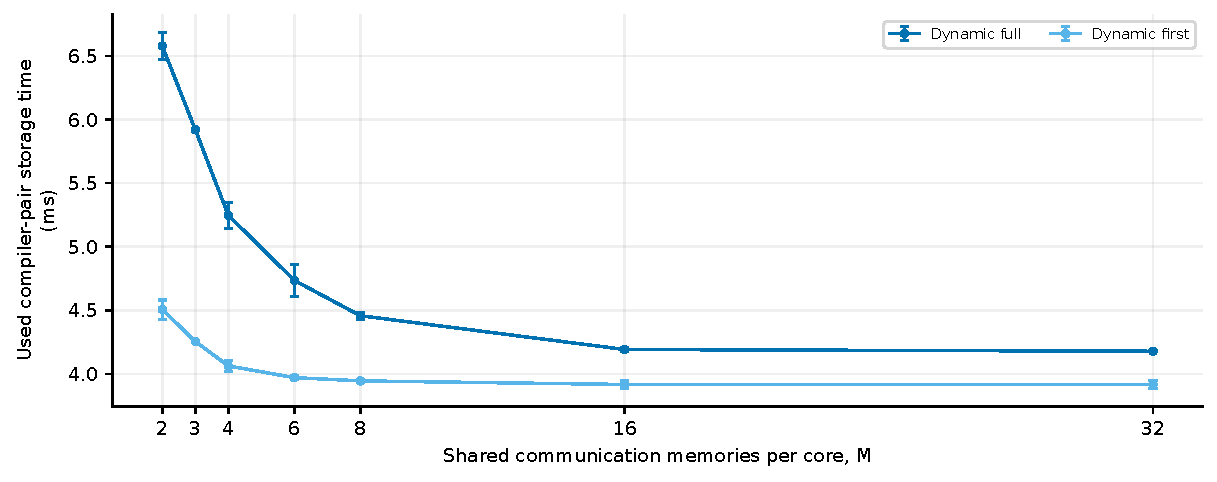
\includegraphics[width=.94\linewidth,height=.255\textheight,keepaspectratio]{figures/memory/mesh_xy_average_storage_time_ms.pdf}\captionof{figure}{Run-level mean and sample SD. Shared trace aliases are counted once.}\end{center}
\begin{center}{\scriptsize\setlength{\tabcolsep}{3pt}
\begin{tabular}{lrrrrr}
\toprule
M & ODG & CGP & ACGP & Dynamic full & Dynamic first \\
\midrule
2 & n/a & n/a & n/a & $6.578\pm0.107$ & $4.506\pm0.075$ \\
3 & n/a & n/a & n/a & $5.921\pm0.001$ & $4.256\pm0.009$ \\
4 & n/a & n/a & n/a & $5.247\pm0.103$ & $4.063\pm0.041$ \\
6 & n/a & n/a & n/a & $4.735\pm0.124$ & $3.971\pm0.014$ \\
8 & n/a & n/a & n/a & $4.458\pm0.026$ & $3.945\pm0.014$ \\
16 & n/a & n/a & n/a & $4.192\pm0.014$ & $3.917\pm0.034$ \\
32 & n/a & n/a & n/a & $4.178\pm0.003$ & $3.917\pm0.034$ \\
\bottomrule\end{tabular}}
\captionof{table}{Mean $\pm$ sample SD; n/a denotes a metric outside that policy's instrumentation.}
{\footnotesize\href{https://github.com/sanjeevkrishnaa/Compiler-Driven-ACE/blob/codex/ace-scheduler-correctness/docs/latex/qft96_final/data/memory_mesh_xy_average_storage_time_ms.csv}{Exact CSV values and sample counts}}
\end{center}
\clearpage
\subsection*{Delivered-hop throughput}
\begin{center}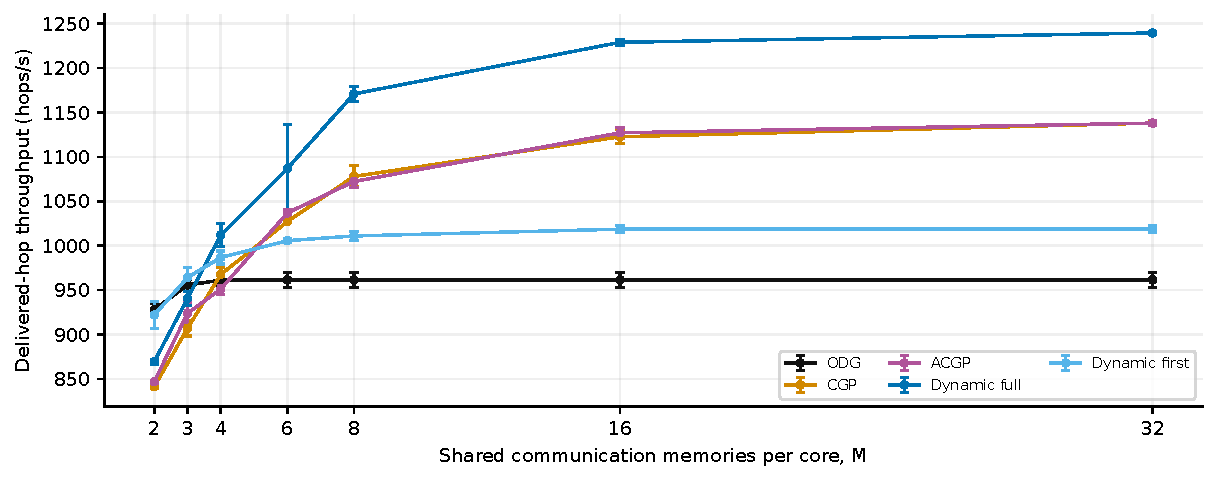
\includegraphics[width=.94\linewidth,height=.255\textheight,keepaspectratio]{figures/memory/mesh_xy_hop_throughput_s.pdf}\captionof{figure}{Run-level mean and sample SD. Shared trace aliases are counted once.}\end{center}
\begin{center}{\scriptsize\setlength{\tabcolsep}{3pt}
\begin{tabular}{lrrrrr}
\toprule
M & ODG & CGP & ACGP & Dynamic full & Dynamic first \\
\midrule
2 & $927.92\pm6.83$ & $841.10\pm2.21$ & $846.68\pm1.42$ & $869.42\pm2.63$ & $921.98\pm14.73$ \\
3 & $955.68\pm6.13$ & $907.05\pm8.75$ & $923.90\pm11.97$ & $940.66\pm8.18$ & $964.11\pm11.75$ \\
4 & $961.17\pm7.33$ & $967.59\pm7.40$ & $951.16\pm6.47$ & $1012.03\pm12.59$ & $986.67\pm7.33$ \\
6 & $961.53\pm8.53$ & $1027.05\pm1.16$ & $1036.88\pm3.65$ & $1086.92\pm49.67$ & $1005.60\pm2.32$ \\
8 & $961.53\pm8.53$ & $1077.97\pm11.78$ & $1072.23\pm6.43$ & $1170.85\pm8.65$ & $1010.92\pm5.05$ \\
16 & $961.53\pm8.53$ & $1122.61\pm7.82$ & $1127.05\pm5.86$ & $1228.94\pm3.22$ & $1018.59\pm4.07$ \\
32 & $961.53\pm8.53$ & $1138.05\pm2.96$ & $1138.00\pm2.53$ & $1239.49\pm0.73$ & $1018.59\pm4.07$ \\
\bottomrule\end{tabular}}
\captionof{table}{Mean $\pm$ sample SD; n/a denotes a metric outside that policy's instrumentation.}
{\footnotesize\href{https://github.com/sanjeevkrishnaa/Compiler-Driven-ACE/blob/codex/ace-scheduler-correctness/docs/latex/qft96_final/data/memory_mesh_xy_hop_throughput_s.csv}{Exact CSV values and sample counts}}
\end{center}
\subsection*{Completion fraction}
\begin{center}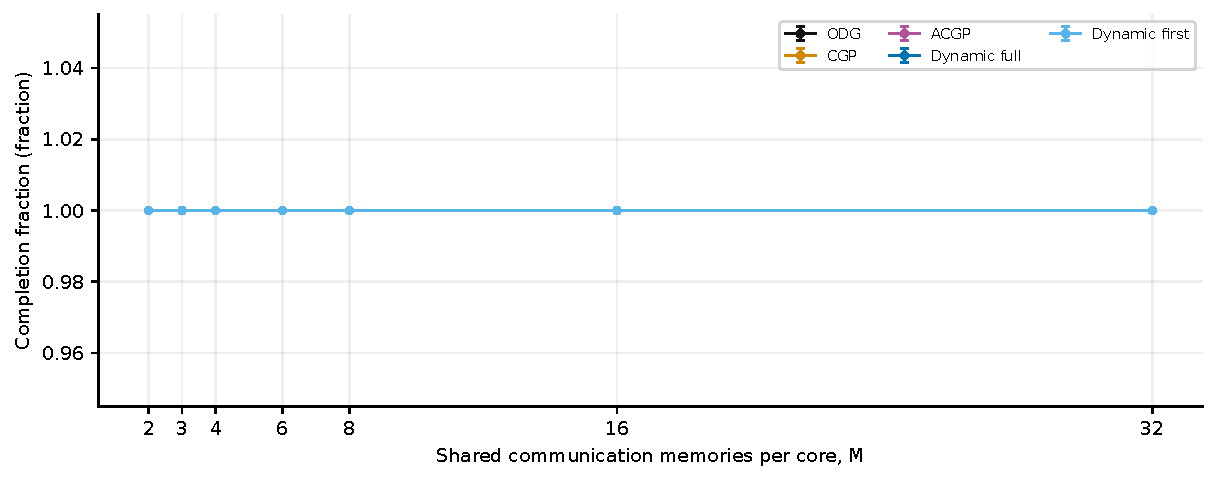
\includegraphics[width=.94\linewidth,height=.255\textheight,keepaspectratio]{figures/memory/mesh_xy_completion_rate.pdf}\captionof{figure}{Run-level mean and sample SD. Shared trace aliases are counted once.}\end{center}
\begin{center}{\scriptsize\setlength{\tabcolsep}{3pt}
\begin{tabular}{lrrrrr}
\toprule
M & ODG & CGP & ACGP & Dynamic full & Dynamic first \\
\midrule
2 & $1.000\pm0.000$ & $1.000\pm0.000$ & $1.000\pm0.000$ & $1.000\pm0.000$ & $1.000\pm0.000$ \\
3 & $1.000\pm0.000$ & $1.000\pm0.000$ & $1.000\pm0.000$ & $1.000\pm0.000$ & $1.000\pm0.000$ \\
4 & $1.000\pm0.000$ & $1.000\pm0.000$ & $1.000\pm0.000$ & $1.000\pm0.000$ & $1.000\pm0.000$ \\
6 & $1.000\pm0.000$ & $1.000\pm0.000$ & $1.000\pm0.000$ & $1.000\pm0.000$ & $1.000\pm0.000$ \\
8 & $1.000\pm0.000$ & $1.000\pm0.000$ & $1.000\pm0.000$ & $1.000\pm0.000$ & $1.000\pm0.000$ \\
16 & $1.000\pm0.000$ & $1.000\pm0.000$ & $1.000\pm0.000$ & $1.000\pm0.000$ & $1.000\pm0.000$ \\
32 & $1.000\pm0.000$ & $1.000\pm0.000$ & $1.000\pm0.000$ & $1.000\pm0.000$ & $1.000\pm0.000$ \\
\bottomrule\end{tabular}}
\captionof{table}{Mean $\pm$ sample SD; n/a denotes a metric outside that policy's instrumentation.}
{\footnotesize\href{https://github.com/sanjeevkrishnaa/Compiler-Driven-ACE/blob/codex/ace-scheduler-correctness/docs/latex/qft96_final/data/memory_mesh_xy_completion_rate.csv}{Exact CSV values and sample counts}}
\end{center}
\clearpage
\subsection*{Maximum admission wait}
\begin{center}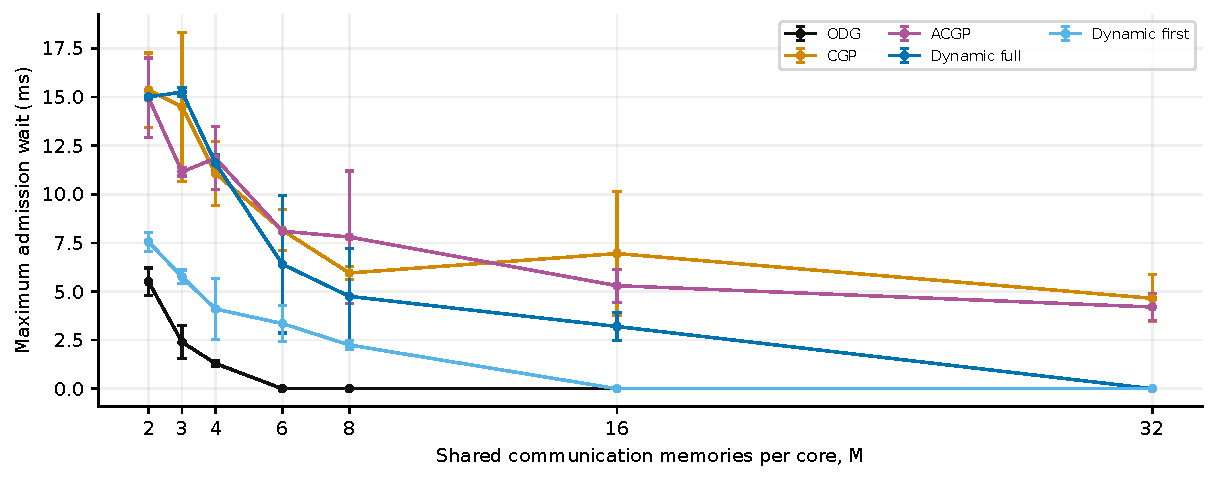
\includegraphics[width=.94\linewidth,height=.255\textheight,keepaspectratio]{figures/memory/mesh_xy_max_admission_wait_ms.pdf}\captionof{figure}{Run-level mean and sample SD. Shared trace aliases are counted once.}\end{center}
\begin{center}{\scriptsize\setlength{\tabcolsep}{3pt}
\begin{tabular}{lrrrrr}
\toprule
M & ODG & CGP & ACGP & Dynamic full & Dynamic first \\
\midrule
2 & $5.500\pm0.707$ & $15.350\pm1.909$ & $14.950\pm2.051$ & $15.000\pm0.000$ & $7.550\pm0.495$ \\
3 & $2.400\pm0.849$ & $14.491\pm3.832$ & $11.150\pm0.212$ & $15.250\pm0.212$ & $5.750\pm0.354$ \\
4 & $1.300\pm0.141$ & $11.067\pm1.651$ & $11.850\pm1.626$ & $11.600\pm0.424$ & $4.100\pm1.556$ \\
6 & $0.0000\pm0.0000$ & $8.150\pm1.061$ & $8.100\pm0.000$ & $6.400\pm3.536$ & $3.350\pm0.919$ \\
8 & $0.0000\pm0.0000$ & $5.950\pm0.354$ & $7.800\pm3.394$ & $4.750\pm2.475$ & $2.250\pm0.212$ \\
16 & $0.0000\pm0.0000$ & $6.950\pm3.182$ & $5.300\pm0.849$ & $3.200\pm0.707$ & $0.0000\pm0.0000$ \\
32 & $0.0000\pm0.0000$ & $4.650\pm1.202$ & $4.200\pm0.707$ & $0.0000\pm0.0000$ & $0.0000\pm0.0000$ \\
\bottomrule\end{tabular}}
\captionof{table}{Mean $\pm$ sample SD; n/a denotes a metric outside that policy's instrumentation.}
{\footnotesize\href{https://github.com/sanjeevkrishnaa/Compiler-Driven-ACE/blob/codex/ace-scheduler-correctness/docs/latex/qft96_final/data/memory_mesh_xy_max_admission_wait_ms.csv}{Exact CSV values and sample counts}}
\end{center}
\subsection*{Requests with admission wait}
\begin{center}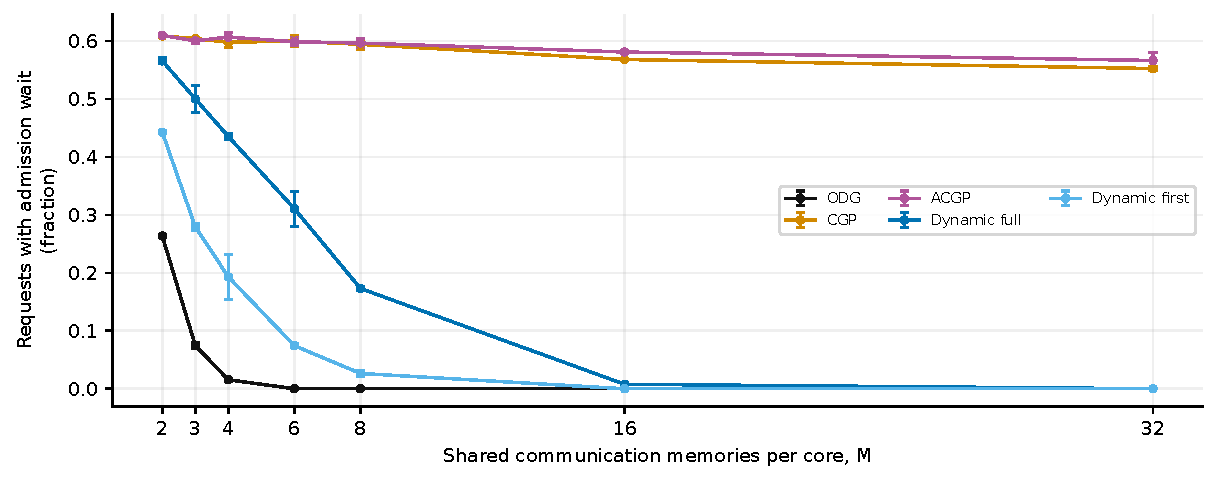
\includegraphics[width=.94\linewidth,height=.255\textheight,keepaspectratio]{figures/memory/mesh_xy_requests_that_waited_fraction.pdf}\captionof{figure}{Run-level mean and sample SD. Shared trace aliases are counted once.}\end{center}
\begin{center}{\scriptsize\setlength{\tabcolsep}{3pt}
\begin{tabular}{lrrrrr}
\toprule
M & ODG & CGP & ACGP & Dynamic full & Dynamic first \\
\midrule
2 & $0.2637\pm0.0033$ & $0.6089\pm0.0007$ & $0.6099\pm0.0022$ & $0.5659\pm0.0053$ & $0.4427\pm0.0022$ \\
3 & $0.0746\pm0.0047$ & $0.6044\pm0.0013$ & $0.6005\pm0.0053$ & $0.5003\pm0.0230$ & $0.2795\pm0.0064$ \\
4 & $0.0155\pm0.0029$ & $0.5980\pm0.0095$ & $0.6069\pm0.0082$ & $0.4354\pm0.0049$ & $0.1931\pm0.0385$ \\
6 & $0.0000\pm0.0000$ & $0.6000\pm0.0100$ & $0.5989\pm0.0071$ & $0.3108\pm0.0301$ & $0.0743\pm0.0033$ \\
8 & $0.0000\pm0.0000$ & $0.5944\pm0.0080$ & $0.5966\pm0.0075$ & $0.1731\pm0.0036$ & $0.0264\pm0.0046$ \\
16 & $0.0000\pm0.0000$ & $0.5682\pm0.0005$ & $0.5811\pm0.0013$ & $0.0077\pm0.0015$ & $0.0000\pm0.0000$ \\
32 & $0.0000\pm0.0000$ & $0.5526\pm0.0036$ & $0.5666\pm0.0135$ & $0.0000\pm0.0000$ & $0.0000\pm0.0000$ \\
\bottomrule\end{tabular}}
\captionof{table}{Mean $\pm$ sample SD; n/a denotes a metric outside that policy's instrumentation.}
{\footnotesize\href{https://github.com/sanjeevkrishnaa/Compiler-Driven-ACE/blob/codex/ace-scheduler-correctness/docs/latex/qft96_final/data/memory_mesh_xy_requests_that_waited_fraction.csv}{Exact CSV values and sample counts}}
\end{center}
\clearpage
\subsection*{Recorded reservation-setup counter}
\begin{center}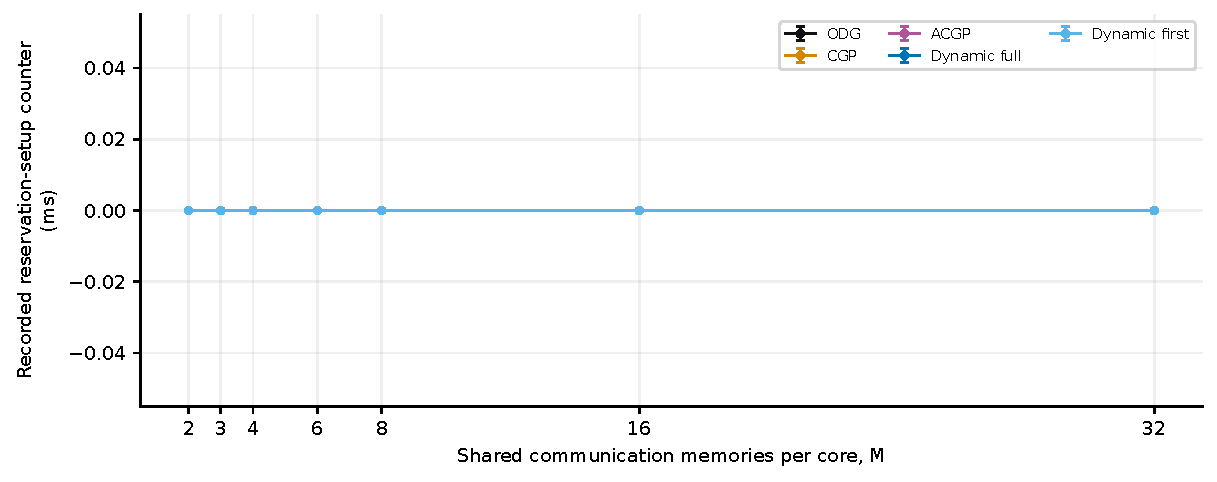
\includegraphics[width=.94\linewidth,height=.255\textheight,keepaspectratio]{figures/memory/mesh_xy_avg_reservation_setup_time_ms.pdf}\captionof{figure}{Run-level mean and sample SD. Shared trace aliases are counted once.}\end{center}
\begin{center}{\scriptsize\setlength{\tabcolsep}{3pt}
\begin{tabular}{lrrrrr}
\toprule
M & ODG & CGP & ACGP & Dynamic full & Dynamic first \\
\midrule
2 & $0.0000\pm0.0000$ & $0.0000\pm0.0000$ & $0.0000\pm0.0000$ & $0.0000\pm0.0000$ & $0.0000\pm0.0000$ \\
3 & $0.0000\pm0.0000$ & $0.0000\pm0.0000$ & $0.0000\pm0.0000$ & $0.0000\pm0.0000$ & $0.0000\pm0.0000$ \\
4 & $0.0000\pm0.0000$ & $0.0000\pm0.0000$ & $0.0000\pm0.0000$ & $0.0000\pm0.0000$ & $0.0000\pm0.0000$ \\
6 & $0.0000\pm0.0000$ & $0.0000\pm0.0000$ & $0.0000\pm0.0000$ & $0.0000\pm0.0000$ & $0.0000\pm0.0000$ \\
8 & $0.0000\pm0.0000$ & $0.0000\pm0.0000$ & $0.0000\pm0.0000$ & $0.0000\pm0.0000$ & $0.0000\pm0.0000$ \\
16 & $0.0000\pm0.0000$ & $0.0000\pm0.0000$ & $0.0000\pm0.0000$ & $0.0000\pm0.0000$ & $0.0000\pm0.0000$ \\
32 & $0.0000\pm0.0000$ & $0.0000\pm0.0000$ & $0.0000\pm0.0000$ & $0.0000\pm0.0000$ & $0.0000\pm0.0000$ \\
\bottomrule\end{tabular}}
\captionof{table}{Mean $\pm$ sample SD; n/a denotes a metric outside that policy's instrumentation.}
{\footnotesize\href{https://github.com/sanjeevkrishnaa/Compiler-Driven-ACE/blob/codex/ace-scheduler-correctness/docs/latex/qft96_final/data/memory_mesh_xy_avg_reservation_setup_time_ms.csv}{Exact CSV values and sample counts}}
\end{center}
\subsection*{Mean generation/service time}
\begin{center}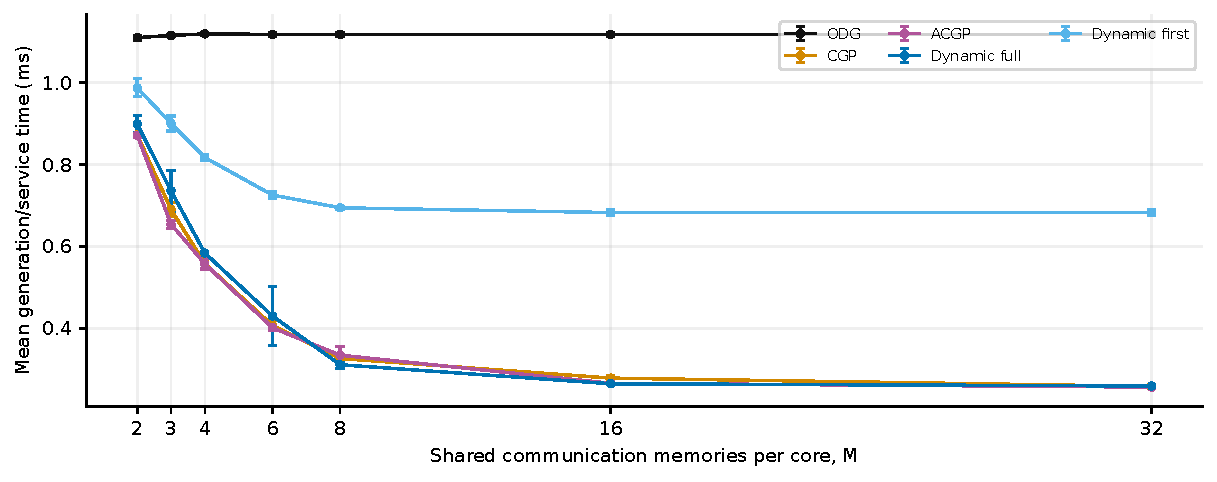
\includegraphics[width=.94\linewidth,height=.255\textheight,keepaspectratio]{figures/memory/mesh_xy_avg_entanglement_generation_time_ms.pdf}\captionof{figure}{Run-level mean and sample SD. Shared trace aliases are counted once.}\end{center}
\begin{center}{\scriptsize\setlength{\tabcolsep}{3pt}
\begin{tabular}{lrrrrr}
\toprule
M & ODG & CGP & ACGP & Dynamic full & Dynamic first \\
\midrule
2 & $1.110\pm0.006$ & $0.8724\pm0.0038$ & $0.8709\pm0.0047$ & $0.8989\pm0.0212$ & $0.9872\pm0.0219$ \\
3 & $1.115\pm0.003$ & $0.6898\pm0.0181$ & $0.6541\pm0.0098$ & $0.7355\pm0.0504$ & $0.9000\pm0.0183$ \\
4 & $1.119\pm0.004$ & $0.5576\pm0.0023$ & $0.5571\pm0.0126$ & $0.5836\pm0.0046$ & $0.8167\pm0.0071$ \\
6 & $1.117\pm0.004$ & $0.4067\pm0.0117$ & $0.4009\pm0.0077$ & $0.4297\pm0.0714$ & $0.7252\pm0.0077$ \\
8 & $1.117\pm0.004$ & $0.3261\pm0.0043$ & $0.3341\pm0.0222$ & $0.3108\pm0.0082$ & $0.6940\pm0.0039$ \\
16 & $1.117\pm0.004$ & $0.2780\pm0.0059$ & $0.2654\pm0.0039$ & $0.2643\pm0.0018$ & $0.6823\pm0.0078$ \\
32 & $1.117\pm0.004$ & $0.2577\pm0.0057$ & $0.2561\pm0.0004$ & $0.2587\pm0.0006$ & $0.6823\pm0.0078$ \\
\bottomrule\end{tabular}}
\captionof{table}{Mean $\pm$ sample SD; n/a denotes a metric outside that policy's instrumentation.}
{\footnotesize\href{https://github.com/sanjeevkrishnaa/Compiler-Driven-ACE/blob/codex/ace-scheduler-correctness/docs/latex/qft96_final/data/memory_mesh_xy_avg_entanglement_generation_time_ms.csv}{Exact CSV values and sample counts}}
\end{center}
\clearpage
\subsection*{Recorded retry-wait time}
\begin{center}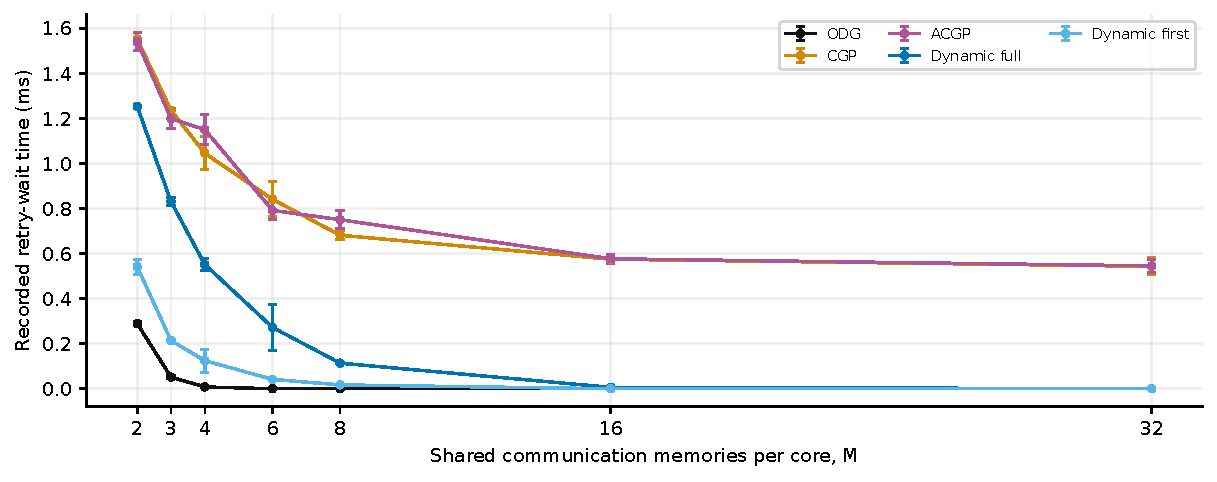
\includegraphics[width=.94\linewidth,height=.255\textheight,keepaspectratio]{figures/memory/mesh_xy_avg_retry_wait_time_ms.pdf}\captionof{figure}{Run-level mean and sample SD. Shared trace aliases are counted once.}\end{center}
\begin{center}{\scriptsize\setlength{\tabcolsep}{3pt}
\begin{tabular}{lrrrrr}
\toprule
M & ODG & CGP & ACGP & Dynamic full & Dynamic first \\
\midrule
2 & $0.2891\pm0.0096$ & $1.552\pm0.004$ & $1.541\pm0.041$ & $1.254\pm0.005$ & $0.5419\pm0.0332$ \\
3 & $0.0517\pm0.0057$ & $1.236\pm0.002$ & $1.200\pm0.044$ & $0.8305\pm0.0186$ & $0.2138\pm0.0034$ \\
4 & $0.0080\pm0.0022$ & $1.045\pm0.073$ & $1.151\pm0.066$ & $0.5515\pm0.0248$ & $0.1248\pm0.0514$ \\
6 & $0.0000\pm0.0000$ & $0.8413\pm0.0774$ & $0.7919\pm0.0409$ & $0.2724\pm0.1025$ & $0.0418\pm0.0052$ \\
8 & $0.0000\pm0.0000$ & $0.6815\pm0.0193$ & $0.7503\pm0.0395$ & $0.1137\pm0.0024$ & $0.0171\pm0.0013$ \\
16 & $0.0000\pm0.0000$ & $0.5749\pm0.0055$ & $0.5770\pm0.0191$ & $0.0062\pm0.0002$ & $0.0000\pm0.0000$ \\
32 & $0.0000\pm0.0000$ & $0.5433\pm0.0373$ & $0.5454\pm0.0282$ & $0.0000\pm0.0000$ & $0.0000\pm0.0000$ \\
\bottomrule\end{tabular}}
\captionof{table}{Mean $\pm$ sample SD; n/a denotes a metric outside that policy's instrumentation.}
{\footnotesize\href{https://github.com/sanjeevkrishnaa/Compiler-Driven-ACE/blob/codex/ace-scheduler-correctness/docs/latex/qft96_final/data/memory_mesh_xy_avg_retry_wait_time_ms.csv}{Exact CSV values and sample counts}}
\end{center}
\subsection*{Request retries}
\begin{center}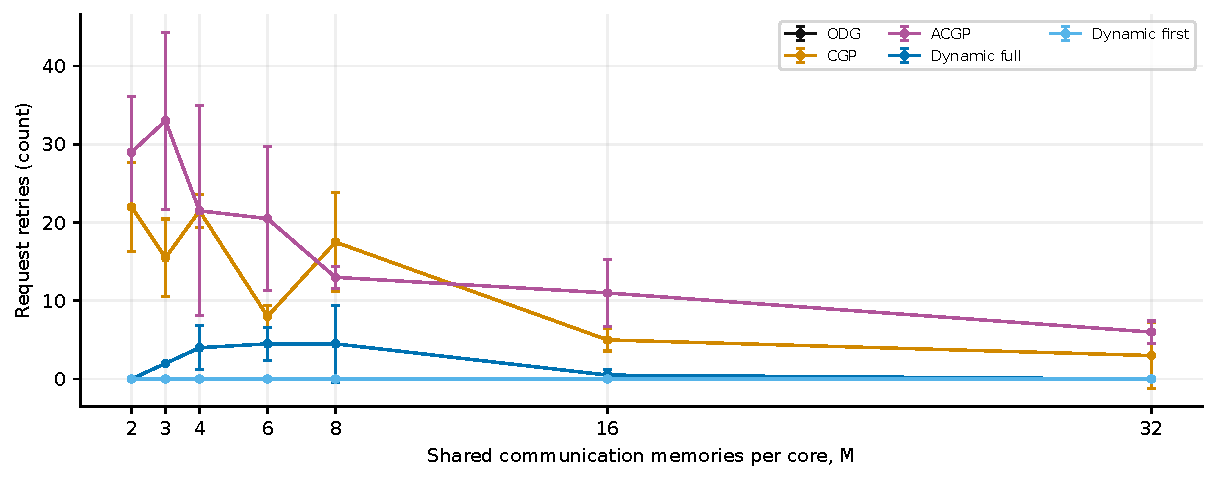
\includegraphics[width=.94\linewidth,height=.255\textheight,keepaspectratio]{figures/memory/mesh_xy_total_retries.pdf}\captionof{figure}{Run-level mean and sample SD. Shared trace aliases are counted once.}\end{center}
\begin{center}{\scriptsize\setlength{\tabcolsep}{3pt}
\begin{tabular}{lrrrrr}
\toprule
M & ODG & CGP & ACGP & Dynamic full & Dynamic first \\
\midrule
2 & $0.0000\pm0.0000$ & $22.000\pm5.657$ & $29.000\pm7.071$ & $0.0000\pm0.0000$ & $0.0000\pm0.0000$ \\
3 & $0.0000\pm0.0000$ & $15.500\pm4.950$ & $33.000\pm11.314$ & $2.000\pm0.000$ & $0.0000\pm0.0000$ \\
4 & $0.0000\pm0.0000$ & $21.500\pm2.121$ & $21.500\pm13.435$ & $4.000\pm2.828$ & $0.0000\pm0.0000$ \\
6 & $0.0000\pm0.0000$ & $8.000\pm1.414$ & $20.500\pm9.192$ & $4.500\pm2.121$ & $0.0000\pm0.0000$ \\
8 & $0.0000\pm0.0000$ & $17.500\pm6.364$ & $13.000\pm1.414$ & $4.500\pm4.950$ & $0.0000\pm0.0000$ \\
16 & $0.0000\pm0.0000$ & $5.000\pm1.414$ & $11.000\pm4.243$ & $0.5000\pm0.7071$ & $0.0000\pm0.0000$ \\
32 & $0.0000\pm0.0000$ & $3.000\pm4.243$ & $6.000\pm1.414$ & $0.0000\pm0.0000$ & $0.0000\pm0.0000$ \\
\bottomrule\end{tabular}}
\captionof{table}{Mean $\pm$ sample SD; n/a denotes a metric outside that policy's instrumentation.}
{\footnotesize\href{https://github.com/sanjeevkrishnaa/Compiler-Driven-ACE/blob/codex/ace-scheduler-correctness/docs/latex/qft96_final/data/memory_mesh_xy_total_retries.csv}{Exact CSV values and sample counts}}
\end{center}
\clearpage
\subsection*{Requests with retries}
\begin{center}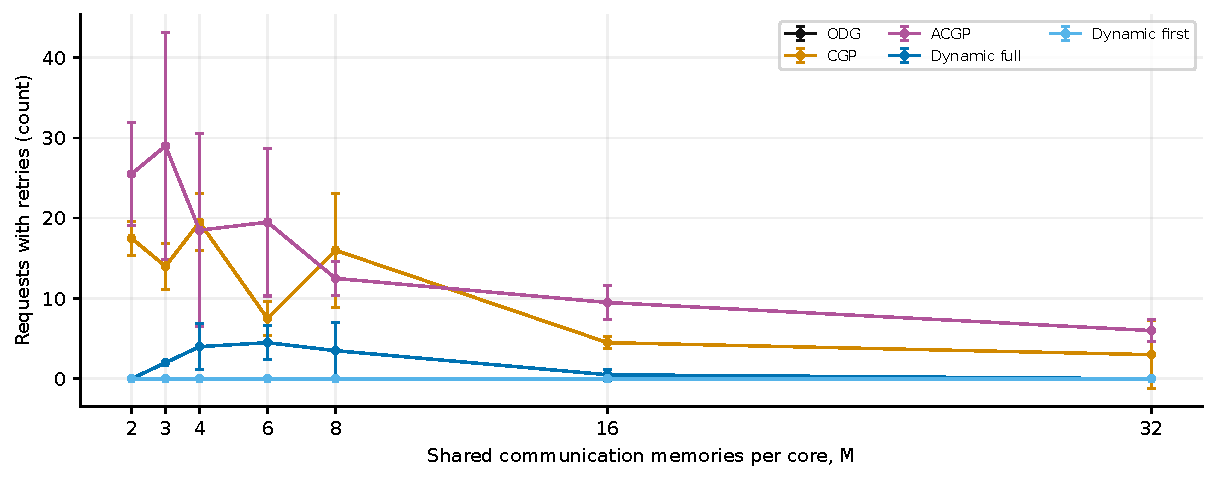
\includegraphics[width=.94\linewidth,height=.255\textheight,keepaspectratio]{figures/memory/mesh_xy_requests_with_retries.pdf}\captionof{figure}{Run-level mean and sample SD. Shared trace aliases are counted once.}\end{center}
\begin{center}{\scriptsize\setlength{\tabcolsep}{3pt}
\begin{tabular}{lrrrrr}
\toprule
M & ODG & CGP & ACGP & Dynamic full & Dynamic first \\
\midrule
2 & $0.0000\pm0.0000$ & $17.500\pm2.121$ & $25.500\pm6.364$ & $0.0000\pm0.0000$ & $0.0000\pm0.0000$ \\
3 & $0.0000\pm0.0000$ & $14.000\pm2.828$ & $29.000\pm14.142$ & $2.000\pm0.000$ & $0.0000\pm0.0000$ \\
4 & $0.0000\pm0.0000$ & $19.500\pm3.536$ & $18.500\pm12.021$ & $4.000\pm2.828$ & $0.0000\pm0.0000$ \\
6 & $0.0000\pm0.0000$ & $7.500\pm2.121$ & $19.500\pm9.192$ & $4.500\pm2.121$ & $0.0000\pm0.0000$ \\
8 & $0.0000\pm0.0000$ & $16.000\pm7.071$ & $12.500\pm2.121$ & $3.500\pm3.536$ & $0.0000\pm0.0000$ \\
16 & $0.0000\pm0.0000$ & $4.500\pm0.707$ & $9.500\pm2.121$ & $0.5000\pm0.7071$ & $0.0000\pm0.0000$ \\
32 & $0.0000\pm0.0000$ & $3.000\pm4.243$ & $6.000\pm1.414$ & $0.0000\pm0.0000$ & $0.0000\pm0.0000$ \\
\bottomrule\end{tabular}}
\captionof{table}{Mean $\pm$ sample SD; n/a denotes a metric outside that policy's instrumentation.}
{\footnotesize\href{https://github.com/sanjeevkrishnaa/Compiler-Driven-ACE/blob/codex/ace-scheduler-correctness/docs/latex/qft96_final/data/memory_mesh_xy_requests_with_retries.csv}{Exact CSV values and sample counts}}
\end{center}
\subsection*{Native-protocol generated-pair counter}
\begin{center}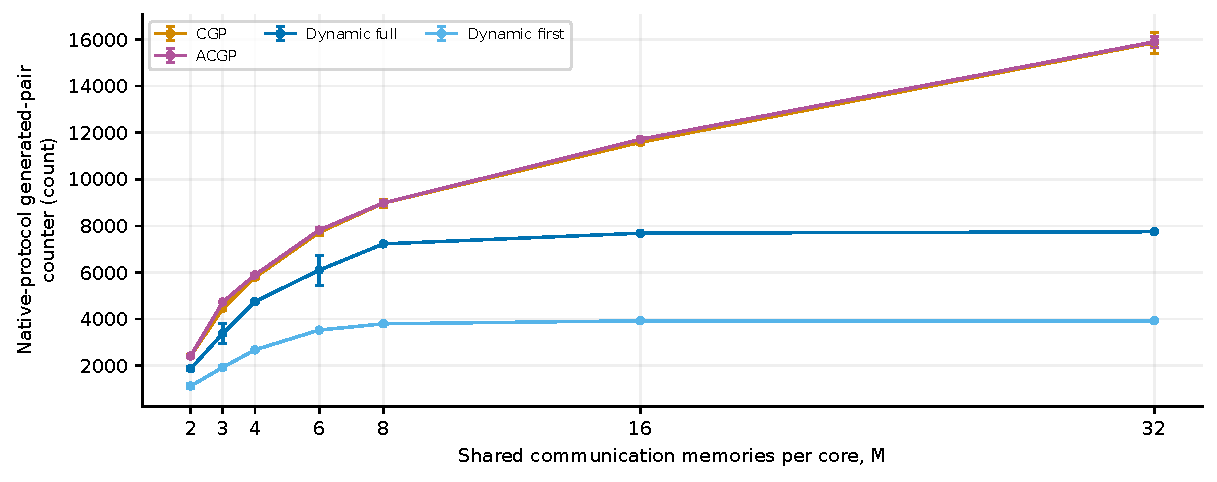
\includegraphics[width=.94\linewidth,height=.255\textheight,keepaspectratio]{figures/memory/mesh_xy_protocol_generated_pairs.pdf}\captionof{figure}{Run-level mean and sample SD. Shared trace aliases are counted once.}\end{center}
\begin{center}{\scriptsize\setlength{\tabcolsep}{3pt}
\begin{tabular}{lrrrrr}
\toprule
M & ODG & CGP & ACGP & Dynamic full & Dynamic first \\
\midrule
2 & n/a & $2424.00\pm39.60$ & $2420.00\pm67.88$ & $1870.00\pm90.51$ & $1129.00\pm117.38$ \\
3 & n/a & $4458.00\pm67.88$ & $4734.00\pm11.31$ & $3385.00\pm442.65$ & $1931.00\pm89.10$ \\
4 & n/a & $5794.00\pm65.05$ & $5895.00\pm80.61$ & $4751.00\pm32.53$ & $2681.00\pm24.04$ \\
6 & n/a & $7725.00\pm142.84$ & $7821.00\pm120.21$ & $6101.00\pm637.81$ & $3530.00\pm36.77$ \\
8 & n/a & $8983.00\pm171.12$ & $8987.00\pm111.72$ & $7230.00\pm16.97$ & $3799.00\pm7.07$ \\
16 & n/a & $11592.00\pm76.37$ & $11718.00\pm84.85$ & $7689.00\pm21.21$ & $3930.00\pm0.00$ \\
32 & n/a & $15865.00\pm445.48$ & $15902.00\pm243.24$ & $7752.00\pm0.00$ & $3930.00\pm0.00$ \\
\bottomrule\end{tabular}}
\captionof{table}{Mean $\pm$ sample SD; n/a denotes a metric outside that policy's instrumentation.}
{\footnotesize\href{https://github.com/sanjeevkrishnaa/Compiler-Driven-ACE/blob/codex/ace-scheduler-correctness/docs/latex/qft96_final/data/memory_mesh_xy_protocol_generated_pairs.csv}{Exact CSV values and sample counts}}
\end{center}
\clearpage
\subsection*{Native-protocol used-pair counter}
\begin{center}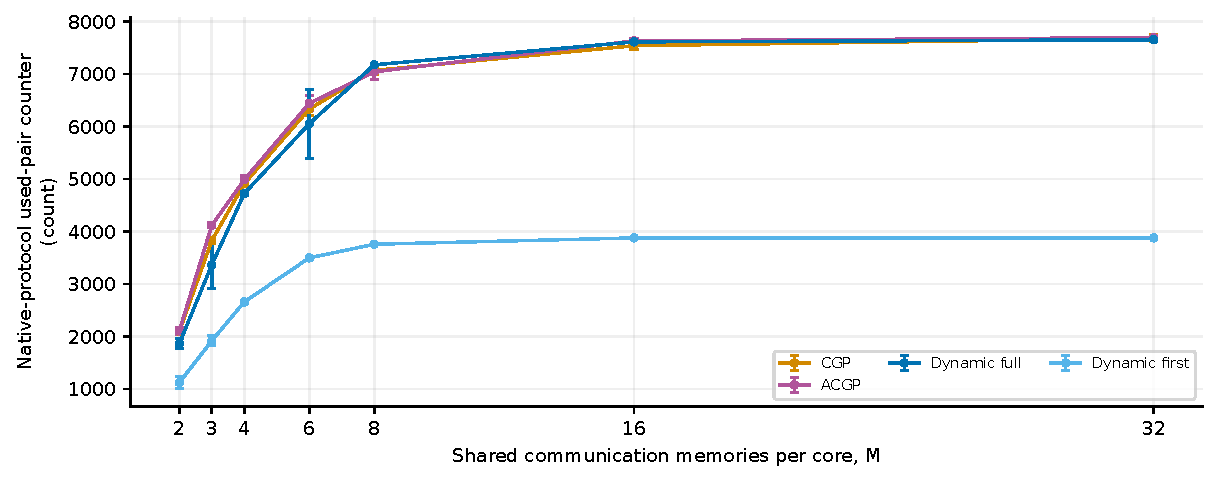
\includegraphics[width=.94\linewidth,height=.255\textheight,keepaspectratio]{figures/memory/mesh_xy_protocol_used_pairs.pdf}\captionof{figure}{Run-level mean and sample SD. Shared trace aliases are counted once.}\end{center}
\begin{center}{\scriptsize\setlength{\tabcolsep}{3pt}
\begin{tabular}{lrrrrr}
\toprule
M & ODG & CGP & ACGP & Dynamic full & Dynamic first \\
\midrule
2 & n/a & $2094.00\pm36.77$ & $2106.00\pm59.40$ & $1862.00\pm93.34$ & $1121.00\pm120.21$ \\
3 & n/a & $3827.00\pm63.64$ & $4117.00\pm46.67$ & $3366.00\pm452.55$ & $1916.00\pm93.34$ \\
4 & n/a & $4911.00\pm18.38$ & $4986.00\pm82.02$ & $4724.00\pm33.94$ & $2658.00\pm25.46$ \\
6 & n/a & $6335.00\pm128.69$ & $6442.00\pm141.42$ & $6053.00\pm657.61$ & $3497.00\pm29.70$ \\
8 & n/a & $7070.00\pm67.88$ & $7044.00\pm147.08$ & $7177.00\pm12.73$ & $3757.00\pm1.41$ \\
16 & n/a & $7541.00\pm69.30$ & $7632.00\pm48.08$ & $7614.00\pm25.46$ & $3878.00\pm2.83$ \\
32 & n/a & $7684.00\pm65.05$ & $7696.00\pm16.97$ & $7655.00\pm12.73$ & $3878.00\pm2.83$ \\
\bottomrule\end{tabular}}
\captionof{table}{Mean $\pm$ sample SD; n/a denotes a metric outside that policy's instrumentation.}
{\footnotesize\href{https://github.com/sanjeevkrishnaa/Compiler-Driven-ACE/blob/codex/ace-scheduler-correctness/docs/latex/qft96_final/data/memory_mesh_xy_protocol_used_pairs.csv}{Exact CSV values and sample counts}}
\end{center}
\subsection*{Native-protocol unused-pair counter}
\begin{center}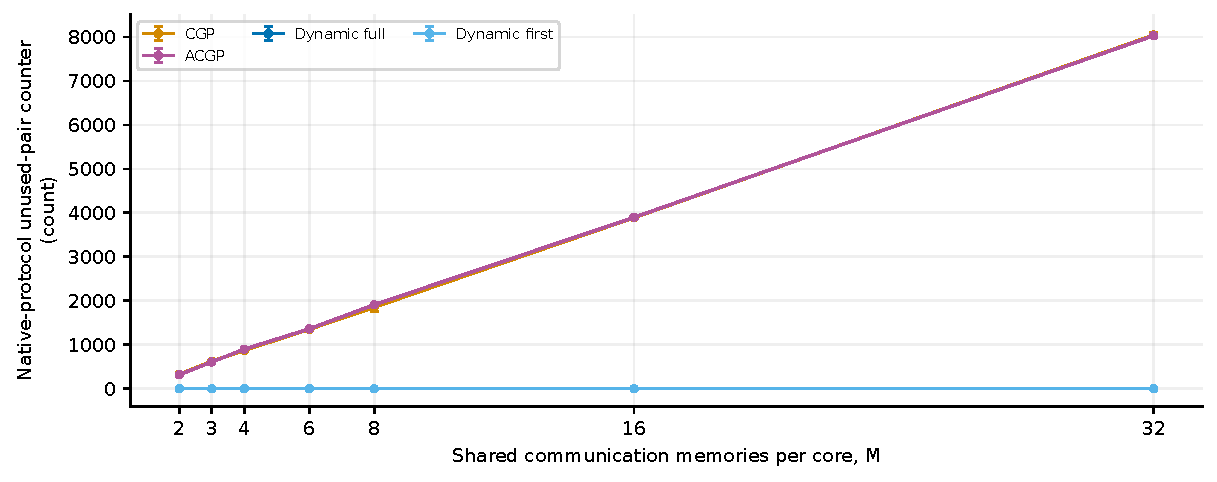
\includegraphics[width=.94\linewidth,height=.255\textheight,keepaspectratio]{figures/memory/mesh_xy_protocol_unused_pairs.pdf}\captionof{figure}{Run-level mean and sample SD. Shared trace aliases are counted once.}\end{center}
\begin{center}{\scriptsize\setlength{\tabcolsep}{3pt}
\begin{tabular}{lrrrrr}
\toprule
M & ODG & CGP & ACGP & Dynamic full & Dynamic first \\
\midrule
2 & n/a & $331.00\pm4.24$ & $319.00\pm4.24$ & $0.0000\pm0.0000$ & $0.0000\pm0.0000$ \\
3 & n/a & $623.00\pm12.73$ & $609.00\pm35.36$ & $0.0000\pm0.0000$ & $0.0000\pm0.0000$ \\
4 & n/a & $873.00\pm32.53$ & $900.00\pm0.00$ & $0.0000\pm0.0000$ & $0.0000\pm0.0000$ \\
6 & n/a & $1351.00\pm15.56$ & $1361.00\pm9.90$ & $0.0000\pm0.0000$ & $0.0000\pm0.0000$ \\
8 & n/a & $1853.00\pm89.10$ & $1910.00\pm31.11$ & $0.0000\pm0.0000$ & $0.0000\pm0.0000$ \\
16 & n/a & $3890.00\pm28.28$ & $3898.00\pm25.46$ & $0.0000\pm0.0000$ & $0.0000\pm0.0000$ \\
32 & n/a & $8042.00\pm62.23$ & $8029.00\pm29.70$ & $0.0000\pm0.0000$ & $0.0000\pm0.0000$ \\
\bottomrule\end{tabular}}
\captionof{table}{Mean $\pm$ sample SD; n/a denotes a metric outside that policy's instrumentation.}
{\footnotesize\href{https://github.com/sanjeevkrishnaa/Compiler-Driven-ACE/blob/codex/ace-scheduler-correctness/docs/latex/qft96_final/data/memory_mesh_xy_protocol_unused_pairs.csv}{Exact CSV values and sample counts}}
\end{center}
\clearpage
\subsection*{Scheduled compiler preparations}
\begin{center}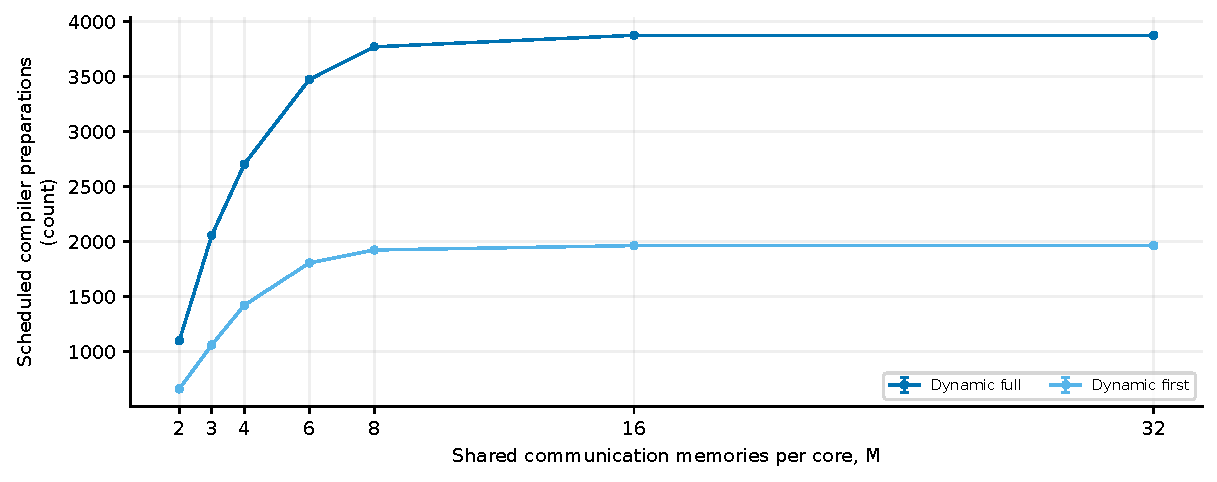
\includegraphics[width=.94\linewidth,height=.255\textheight,keepaspectratio]{figures/memory/mesh_xy_scheduled_preparations.pdf}\captionof{figure}{Run-level mean and sample SD. Shared trace aliases are counted once.}\end{center}
\begin{center}{\scriptsize\setlength{\tabcolsep}{3pt}
\begin{tabular}{lrrrrr}
\toprule
M & ODG & CGP & ACGP & Dynamic full & Dynamic first \\
\midrule
2 & n/a & n/a & n/a & $1101.00\pm0.00$ & $663.00\pm0.00$ \\
3 & n/a & n/a & n/a & $2059.00\pm0.00$ & $1063.00\pm0.00$ \\
4 & n/a & n/a & n/a & $2704.00\pm0.00$ & $1423.00\pm0.00$ \\
6 & n/a & n/a & n/a & $3474.00\pm0.00$ & $1807.00\pm0.00$ \\
8 & n/a & n/a & n/a & $3771.00\pm0.00$ & $1925.00\pm0.00$ \\
16 & n/a & n/a & n/a & $3876.00\pm0.00$ & $1965.00\pm0.00$ \\
32 & n/a & n/a & n/a & $3876.00\pm0.00$ & $1965.00\pm0.00$ \\
\bottomrule\end{tabular}}
\captionof{table}{Mean $\pm$ sample SD; n/a denotes a metric outside that policy's instrumentation.}
{\footnotesize\href{https://github.com/sanjeevkrishnaa/Compiler-Driven-ACE/blob/codex/ace-scheduler-correctness/docs/latex/qft96_final/data/memory_mesh_xy_scheduled_preparations.csv}{Exact CSV values and sample counts}}
\end{center}
\subsection*{Planner-blocked preparations}
\begin{center}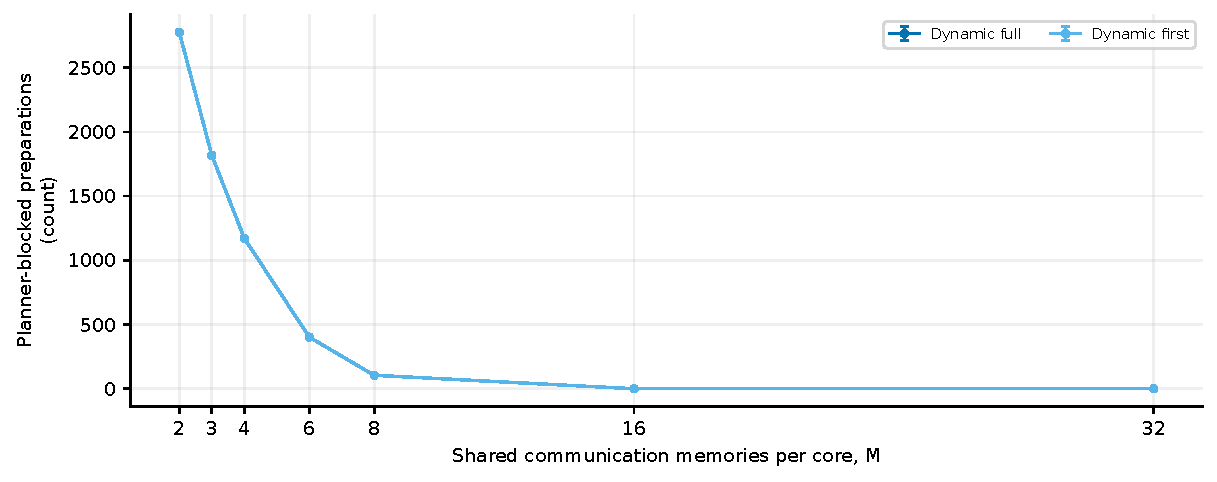
\includegraphics[width=.94\linewidth,height=.255\textheight,keepaspectratio]{figures/memory/mesh_xy_planner_blocked_preparations.pdf}\captionof{figure}{Run-level mean and sample SD. Shared trace aliases are counted once.}\end{center}
\begin{center}{\scriptsize\setlength{\tabcolsep}{3pt}
\begin{tabular}{lrrrrr}
\toprule
M & ODG & CGP & ACGP & Dynamic full & Dynamic first \\
\midrule
2 & n/a & n/a & n/a & $2775.00\pm0.00$ & $2775.00\pm0.00$ \\
3 & n/a & n/a & n/a & $1817.00\pm0.00$ & $1817.00\pm0.00$ \\
4 & n/a & n/a & n/a & $1172.00\pm0.00$ & $1172.00\pm0.00$ \\
6 & n/a & n/a & n/a & $402.00\pm0.00$ & $402.00\pm0.00$ \\
8 & n/a & n/a & n/a & $105.00\pm0.00$ & $105.00\pm0.00$ \\
16 & n/a & n/a & n/a & $0.0000\pm0.0000$ & $0.0000\pm0.0000$ \\
32 & n/a & n/a & n/a & $0.0000\pm0.0000$ & $0.0000\pm0.0000$ \\
\bottomrule\end{tabular}}
\captionof{table}{Mean $\pm$ sample SD; n/a denotes a metric outside that policy's instrumentation.}
{\footnotesize\href{https://github.com/sanjeevkrishnaa/Compiler-Driven-ACE/blob/codex/ace-scheduler-correctness/docs/latex/qft96_final/data/memory_mesh_xy_planner_blocked_preparations.csv}{Exact CSV values and sample counts}}
\end{center}
\clearpage
\subsection*{Planner peak compiler memory}
\begin{center}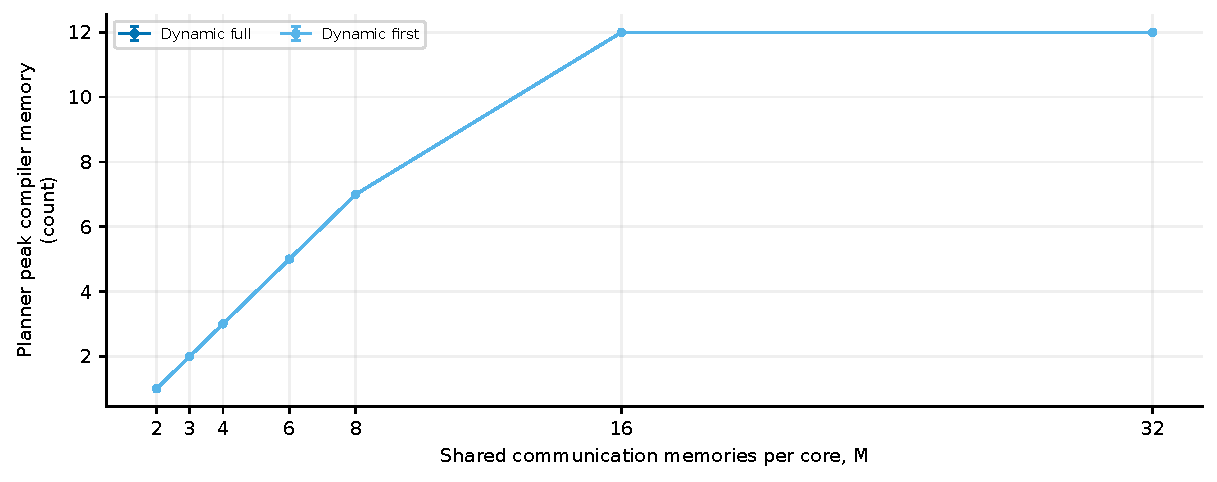
\includegraphics[width=.94\linewidth,height=.255\textheight,keepaspectratio]{figures/memory/mesh_xy_planner_peak_compiler_memory_per_core.pdf}\captionof{figure}{Run-level mean and sample SD. Shared trace aliases are counted once.}\end{center}
\begin{center}{\scriptsize\setlength{\tabcolsep}{3pt}
\begin{tabular}{lrrrrr}
\toprule
M & ODG & CGP & ACGP & Dynamic full & Dynamic first \\
\midrule
2 & n/a & n/a & n/a & $1.000\pm0.000$ & $1.000\pm0.000$ \\
3 & n/a & n/a & n/a & $2.000\pm0.000$ & $2.000\pm0.000$ \\
4 & n/a & n/a & n/a & $3.000\pm0.000$ & $3.000\pm0.000$ \\
6 & n/a & n/a & n/a & $5.000\pm0.000$ & $5.000\pm0.000$ \\
8 & n/a & n/a & n/a & $7.000\pm0.000$ & $7.000\pm0.000$ \\
16 & n/a & n/a & n/a & $12.000\pm0.000$ & $12.000\pm0.000$ \\
32 & n/a & n/a & n/a & $12.000\pm0.000$ & $12.000\pm0.000$ \\
\bottomrule\end{tabular}}
\captionof{table}{Mean $\pm$ sample SD; n/a denotes a metric outside that policy's instrumentation.}
{\footnotesize\href{https://github.com/sanjeevkrishnaa/Compiler-Driven-ACE/blob/codex/ace-scheduler-correctness/docs/latex/qft96_final/data/memory_mesh_xy_planner_peak_compiler_memory_per_core.csv}{Exact CSV values and sample counts}}
\end{center}
\subsection*{Compiler preparation admission attempts}
\begin{center}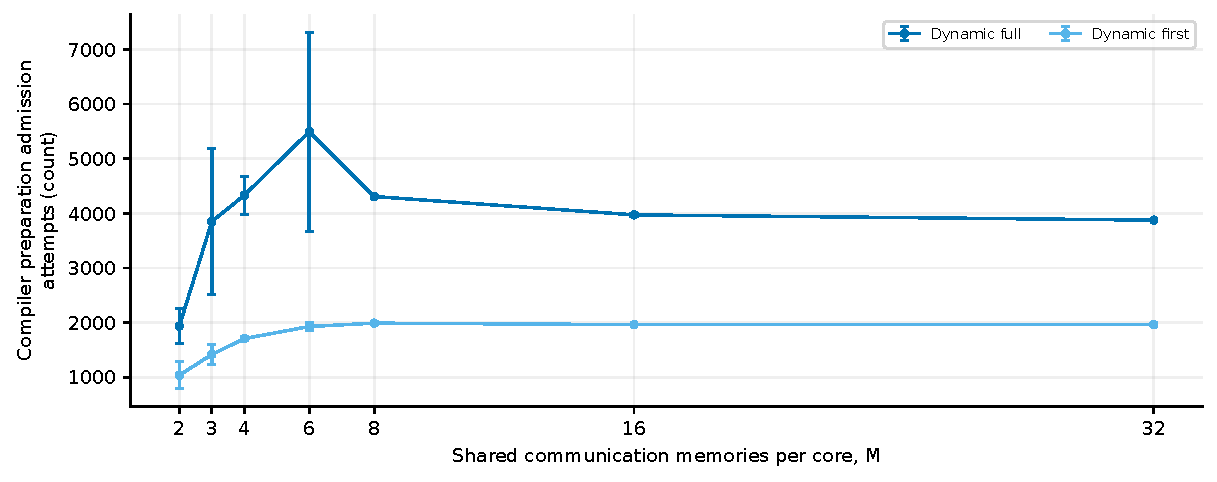
\includegraphics[width=.94\linewidth,height=.255\textheight,keepaspectratio]{figures/memory/mesh_xy_runtime_admission_attempts.pdf}\captionof{figure}{Run-level mean and sample SD. Shared trace aliases are counted once.}\end{center}
\begin{center}{\scriptsize\setlength{\tabcolsep}{3pt}
\begin{tabular}{lrrrrr}
\toprule
M & ODG & CGP & ACGP & Dynamic full & Dynamic first \\
\midrule
2 & n/a & n/a & n/a & $1937.50\pm317.49$ & $1039.00\pm247.49$ \\
3 & n/a & n/a & n/a & $3850.50\pm1332.90$ & $1418.50\pm190.21$ \\
4 & n/a & n/a & n/a & $4331.00\pm352.14$ & $1708.50\pm40.31$ \\
6 & n/a & n/a & n/a & $5494.50\pm1817.97$ & $1930.00\pm74.95$ \\
8 & n/a & n/a & n/a & $4308.00\pm22.63$ & $1992.00\pm21.21$ \\
16 & n/a & n/a & n/a & $3973.00\pm29.70$ & $1965.00\pm0.00$ \\
32 & n/a & n/a & n/a & $3876.00\pm0.00$ & $1965.00\pm0.00$ \\
\bottomrule\end{tabular}}
\captionof{table}{Mean $\pm$ sample SD; n/a denotes a metric outside that policy's instrumentation.}
{\footnotesize\href{https://github.com/sanjeevkrishnaa/Compiler-Driven-ACE/blob/codex/ace-scheduler-correctness/docs/latex/qft96_final/data/memory_mesh_xy_runtime_admission_attempts.csv}{Exact CSV values and sample counts}}
\end{center}
\clearpage
\subsection*{Launched compiler preparations}
\begin{center}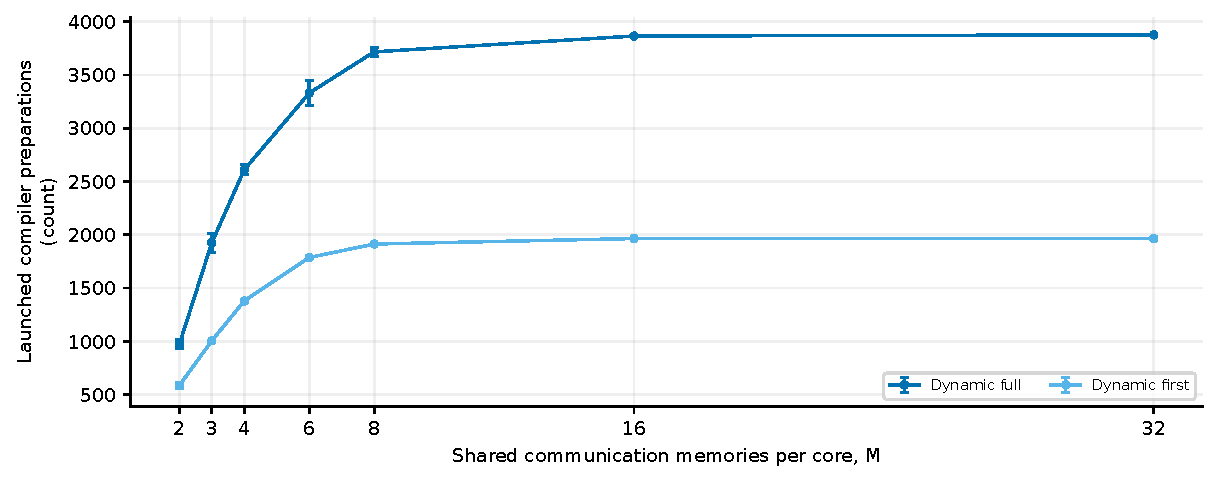
\includegraphics[width=.94\linewidth,height=.255\textheight,keepaspectratio]{figures/memory/mesh_xy_runtime_launched_preparations.pdf}\captionof{figure}{Run-level mean and sample SD. Shared trace aliases are counted once.}\end{center}
\begin{center}{\scriptsize\setlength{\tabcolsep}{3pt}
\begin{tabular}{lrrrrr}
\toprule
M & ODG & CGP & ACGP & Dynamic full & Dynamic first \\
\midrule
2 & n/a & n/a & n/a & $971.50\pm41.72$ & $586.50\pm31.82$ \\
3 & n/a & n/a & n/a & $1926.00\pm89.10$ & $1006.00\pm5.66$ \\
4 & n/a & n/a & n/a & $2611.00\pm49.50$ & $1379.50\pm17.68$ \\
6 & n/a & n/a & n/a & $3330.00\pm114.55$ & $1787.00\pm11.31$ \\
8 & n/a & n/a & n/a & $3716.50\pm40.31$ & $1913.50\pm6.36$ \\
16 & n/a & n/a & n/a & $3865.00\pm5.66$ & $1965.00\pm0.00$ \\
32 & n/a & n/a & n/a & $3876.00\pm0.00$ & $1965.00\pm0.00$ \\
\bottomrule\end{tabular}}
\captionof{table}{Mean $\pm$ sample SD; n/a denotes a metric outside that policy's instrumentation.}
{\footnotesize\href{https://github.com/sanjeevkrishnaa/Compiler-Driven-ACE/blob/codex/ace-scheduler-correctness/docs/latex/qft96_final/data/memory_mesh_xy_runtime_launched_preparations.csv}{Exact CSV values and sample counts}}
\end{center}
\subsection*{Accepted compiler preparations}
\begin{center}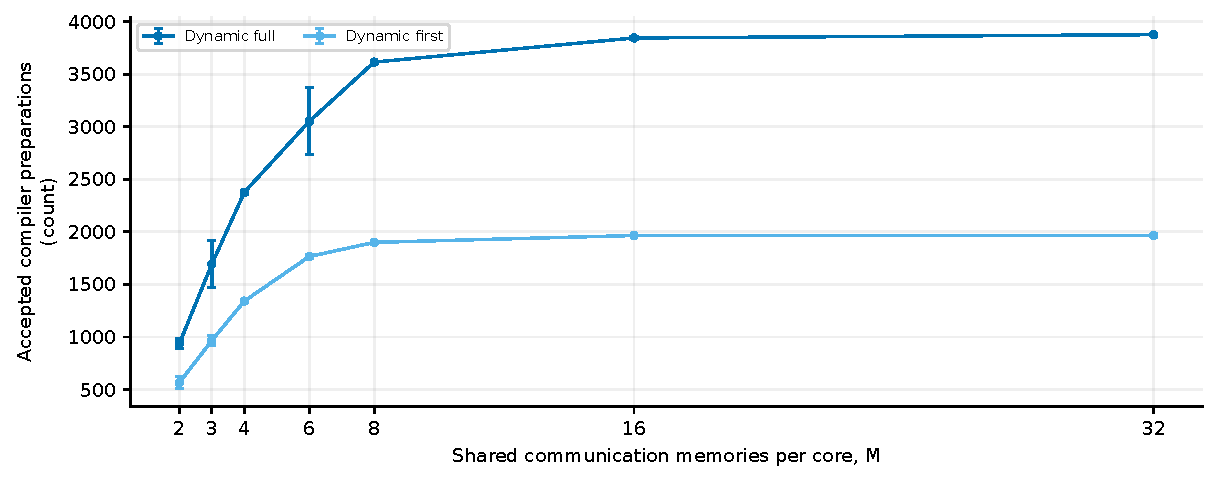
\includegraphics[width=.94\linewidth,height=.255\textheight,keepaspectratio]{figures/memory/mesh_xy_runtime_accepted_preparations.pdf}\captionof{figure}{Run-level mean and sample SD. Shared trace aliases are counted once.}\end{center}
\begin{center}{\scriptsize\setlength{\tabcolsep}{3pt}
\begin{tabular}{lrrrrr}
\toprule
M & ODG & CGP & ACGP & Dynamic full & Dynamic first \\
\midrule
2 & n/a & n/a & n/a & $935.00\pm45.25$ & $564.50\pm58.69$ \\
3 & n/a & n/a & n/a & $1692.50\pm221.32$ & $965.50\pm44.55$ \\
4 & n/a & n/a & n/a & $2375.50\pm16.26$ & $1340.50\pm12.02$ \\
6 & n/a & n/a & n/a & $3050.50\pm318.91$ & $1765.00\pm18.38$ \\
8 & n/a & n/a & n/a & $3615.00\pm8.49$ & $1899.50\pm3.54$ \\
16 & n/a & n/a & n/a & $3844.50\pm10.61$ & $1965.00\pm0.00$ \\
32 & n/a & n/a & n/a & $3876.00\pm0.00$ & $1965.00\pm0.00$ \\
\bottomrule\end{tabular}}
\captionof{table}{Mean $\pm$ sample SD; n/a denotes a metric outside that policy's instrumentation.}
{\footnotesize\href{https://github.com/sanjeevkrishnaa/Compiler-Driven-ACE/blob/codex/ace-scheduler-correctness/docs/latex/qft96_final/data/memory_mesh_xy_runtime_accepted_preparations.csv}{Exact CSV values and sample counts}}
\end{center}
\clearpage
\subsection*{Rejected compiler preparations}
\begin{center}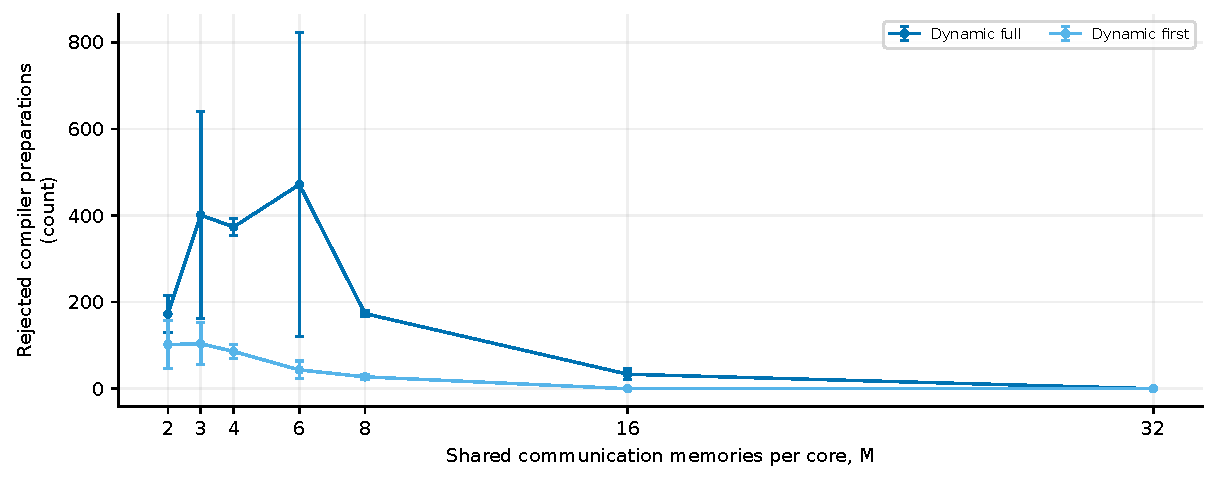
\includegraphics[width=.94\linewidth,height=.255\textheight,keepaspectratio]{figures/memory/mesh_xy_runtime_rejected_preparations.pdf}\captionof{figure}{Run-level mean and sample SD. Shared trace aliases are counted once.}\end{center}
\begin{center}{\scriptsize\setlength{\tabcolsep}{3pt}
\begin{tabular}{lrrrrr}
\toprule
M & ODG & CGP & ACGP & Dynamic full & Dynamic first \\
\midrule
2 & n/a & n/a & n/a & $172.50\pm43.13$ & $102.00\pm55.15$ \\
3 & n/a & n/a & n/a & $401.00\pm239.00$ & $104.00\pm48.08$ \\
4 & n/a & n/a & n/a & $373.50\pm19.09$ & $86.000\pm16.971$ \\
6 & n/a & n/a & n/a & $471.50\pm351.43$ & $43.500\pm20.506$ \\
8 & n/a & n/a & n/a & $173.50\pm6.36$ & $27.500\pm4.950$ \\
16 & n/a & n/a & n/a & $33.500\pm12.021$ & $0.0000\pm0.0000$ \\
32 & n/a & n/a & n/a & $0.0000\pm0.0000$ & $0.0000\pm0.0000$ \\
\bottomrule\end{tabular}}
\captionof{table}{Mean $\pm$ sample SD; n/a denotes a metric outside that policy's instrumentation.}
{\footnotesize\href{https://github.com/sanjeevkrishnaa/Compiler-Driven-ACE/blob/codex/ace-scheduler-correctness/docs/latex/qft96_final/data/memory_mesh_xy_runtime_rejected_preparations.csv}{Exact CSV values and sample counts}}
\end{center}
\subsection*{Compiler-ready request count}
\begin{center}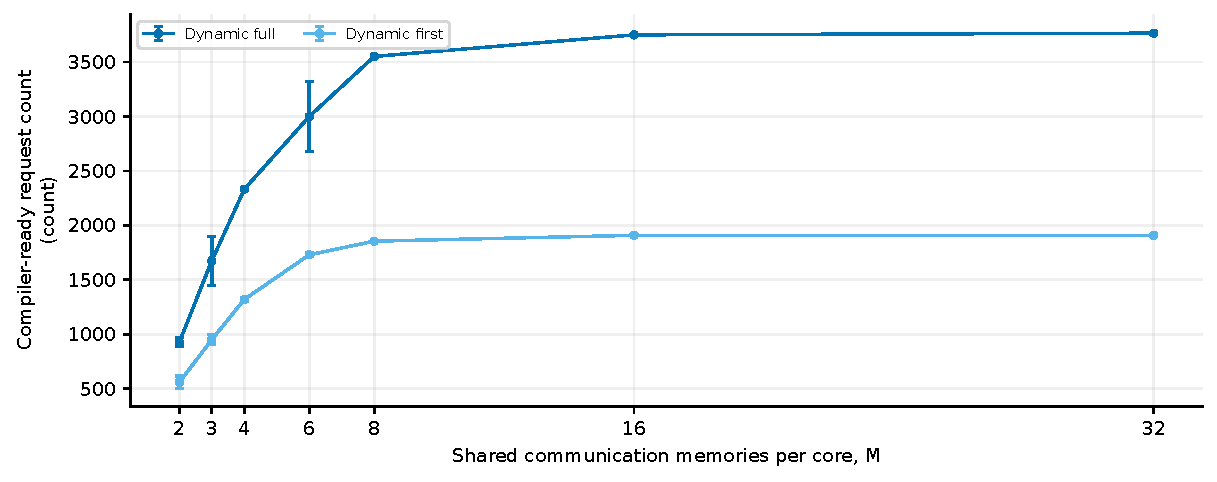
\includegraphics[width=.94\linewidth,height=.255\textheight,keepaspectratio]{figures/memory/mesh_xy_pregenerated_hits.pdf}\captionof{figure}{Run-level mean and sample SD. Shared trace aliases are counted once.}\end{center}
\begin{center}{\scriptsize\setlength{\tabcolsep}{3pt}
\begin{tabular}{lrrrrr}
\toprule
M & ODG & CGP & ACGP & Dynamic full & Dynamic first \\
\midrule
2 & n/a & n/a & n/a & $926.50\pm43.13$ & $557.50\pm58.69$ \\
3 & n/a & n/a & n/a & $1675.00\pm224.86$ & $950.00\pm46.67$ \\
4 & n/a & n/a & n/a & $2332.00\pm2.83$ & $1319.00\pm16.97$ \\
6 & n/a & n/a & n/a & $3000.00\pm323.85$ & $1729.50\pm16.26$ \\
8 & n/a & n/a & n/a & $3551.50\pm4.95$ & $1854.50\pm2.12$ \\
16 & n/a & n/a & n/a & $3750.00\pm1.41$ & $1908.50\pm3.54$ \\
32 & n/a & n/a & n/a & $3765.50\pm7.78$ & $1908.50\pm3.54$ \\
\bottomrule\end{tabular}}
\captionof{table}{Mean $\pm$ sample SD; n/a denotes a metric outside that policy's instrumentation.}
{\footnotesize\href{https://github.com/sanjeevkrishnaa/Compiler-Driven-ACE/blob/codex/ace-scheduler-correctness/docs/latex/qft96_final/data/memory_mesh_xy_pregenerated_hits.csv}{Exact CSV values and sample counts}}
\end{center}
\clearpage
\subsection*{Intended compiler-hit count}
\begin{center}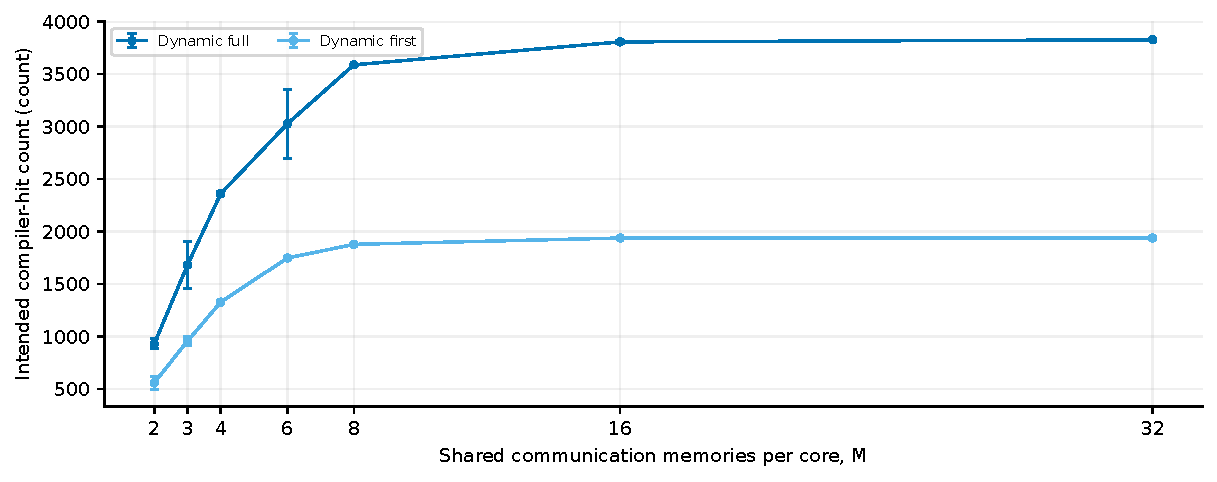
\includegraphics[width=.94\linewidth,height=.255\textheight,keepaspectratio]{figures/memory/mesh_xy_intended_request_hits.pdf}\captionof{figure}{Run-level mean and sample SD. Shared trace aliases are counted once.}\end{center}
\begin{center}{\scriptsize\setlength{\tabcolsep}{3pt}
\begin{tabular}{lrrrrr}
\toprule
M & ODG & CGP & ACGP & Dynamic full & Dynamic first \\
\midrule
2 & n/a & n/a & n/a & $931.00\pm46.67$ & $560.50\pm60.10$ \\
3 & n/a & n/a & n/a & $1683.00\pm226.27$ & $958.00\pm46.67$ \\
4 & n/a & n/a & n/a & $2362.00\pm16.97$ & $1329.00\pm12.73$ \\
6 & n/a & n/a & n/a & $3026.50\pm328.80$ & $1748.50\pm14.85$ \\
8 & n/a & n/a & n/a & $3588.50\pm6.36$ & $1878.50\pm0.71$ \\
16 & n/a & n/a & n/a & $3807.00\pm12.73$ & $1939.00\pm1.41$ \\
32 & n/a & n/a & n/a & $3827.50\pm6.36$ & $1939.00\pm1.41$ \\
\bottomrule\end{tabular}}
\captionof{table}{Mean $\pm$ sample SD; n/a denotes a metric outside that policy's instrumentation.}
{\footnotesize\href{https://github.com/sanjeevkrishnaa/Compiler-Driven-ACE/blob/codex/ace-scheduler-correctness/docs/latex/qft96_final/data/memory_mesh_xy_intended_request_hits.csv}{Exact CSV values and sample counts}}
\end{center}
\subsection*{Compiler-not-ready request count}
\begin{center}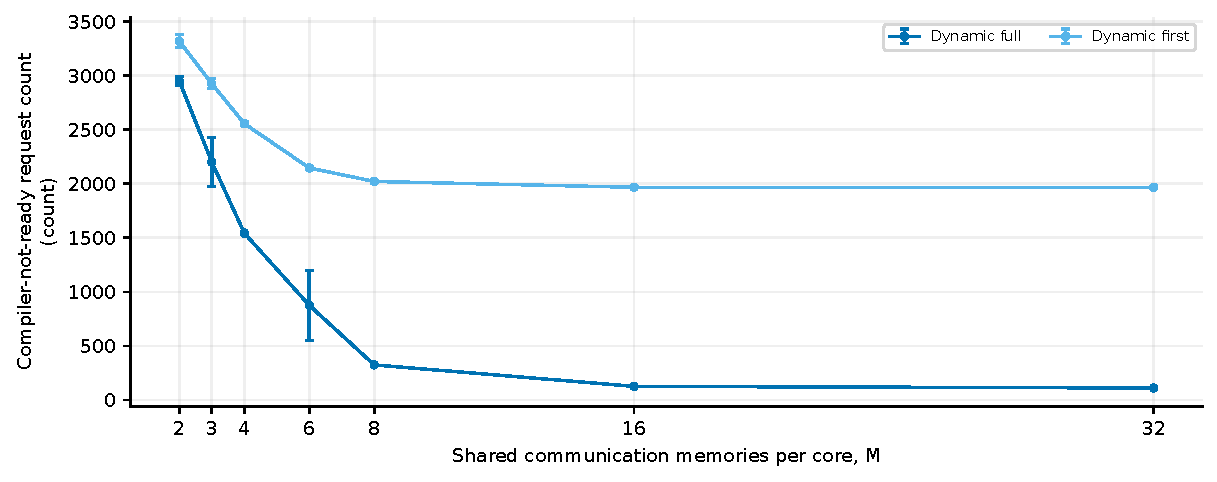
\includegraphics[width=.94\linewidth,height=.255\textheight,keepaspectratio]{figures/memory/mesh_xy_compiler_not_ready_requests.pdf}\captionof{figure}{Run-level mean and sample SD. Shared trace aliases are counted once.}\end{center}
\begin{center}{\scriptsize\setlength{\tabcolsep}{3pt}
\begin{tabular}{lrrrrr}
\toprule
M & ODG & CGP & ACGP & Dynamic full & Dynamic first \\
\midrule
2 & n/a & n/a & n/a & $2949.50\pm43.13$ & $3318.50\pm58.69$ \\
3 & n/a & n/a & n/a & $2201.00\pm224.86$ & $2926.00\pm46.67$ \\
4 & n/a & n/a & n/a & $1544.00\pm2.83$ & $2557.00\pm16.97$ \\
6 & n/a & n/a & n/a & $876.00\pm323.85$ & $2146.50\pm16.26$ \\
8 & n/a & n/a & n/a & $324.50\pm4.95$ & $2021.50\pm2.12$ \\
16 & n/a & n/a & n/a & $126.00\pm1.41$ & $1967.50\pm3.54$ \\
32 & n/a & n/a & n/a & $110.50\pm7.78$ & $1967.50\pm3.54$ \\
\bottomrule\end{tabular}}
\captionof{table}{Mean $\pm$ sample SD; n/a denotes a metric outside that policy's instrumentation.}
{\footnotesize\href{https://github.com/sanjeevkrishnaa/Compiler-Driven-ACE/blob/codex/ace-scheduler-correctness/docs/latex/qft96_final/data/memory_mesh_xy_compiler_not_ready_requests.csv}{Exact CSV values and sample counts}}
\end{center}
\clearpage
\subsection*{Late compiler-pair uses}
\begin{center}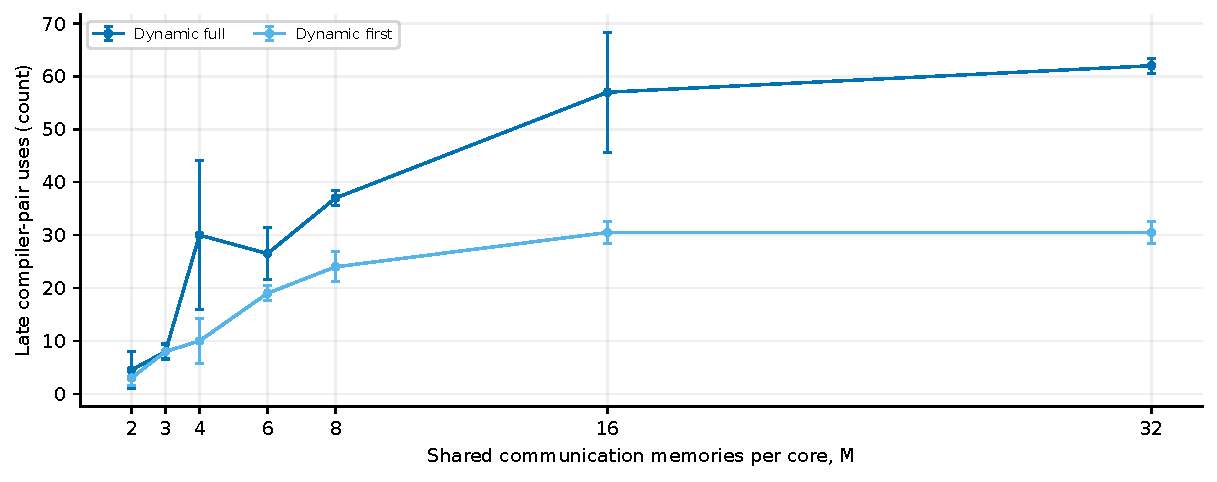
\includegraphics[width=.94\linewidth,height=.255\textheight,keepaspectratio]{figures/memory/mesh_xy_late_compiler_pair_uses.pdf}\captionof{figure}{Run-level mean and sample SD. Shared trace aliases are counted once.}\end{center}
\begin{center}{\scriptsize\setlength{\tabcolsep}{3pt}
\begin{tabular}{lrrrrr}
\toprule
M & ODG & CGP & ACGP & Dynamic full & Dynamic first \\
\midrule
2 & n/a & n/a & n/a & $4.500\pm3.536$ & $3.000\pm1.414$ \\
3 & n/a & n/a & n/a & $8.000\pm1.414$ & $8.000\pm0.000$ \\
4 & n/a & n/a & n/a & $30.000\pm14.142$ & $10.000\pm4.243$ \\
6 & n/a & n/a & n/a & $26.500\pm4.950$ & $19.000\pm1.414$ \\
8 & n/a & n/a & n/a & $37.000\pm1.414$ & $24.000\pm2.828$ \\
16 & n/a & n/a & n/a & $57.000\pm11.314$ & $30.500\pm2.121$ \\
32 & n/a & n/a & n/a & $62.000\pm1.414$ & $30.500\pm2.121$ \\
\bottomrule\end{tabular}}
\captionof{table}{Mean $\pm$ sample SD; n/a denotes a metric outside that policy's instrumentation.}
{\footnotesize\href{https://github.com/sanjeevkrishnaa/Compiler-Driven-ACE/blob/codex/ace-scheduler-correctness/docs/latex/qft96_final/data/memory_mesh_xy_late_compiler_pair_uses.csv}{Exact CSV values and sample counts}}
\end{center}
\subsection*{Compiler fallback count}
\begin{center}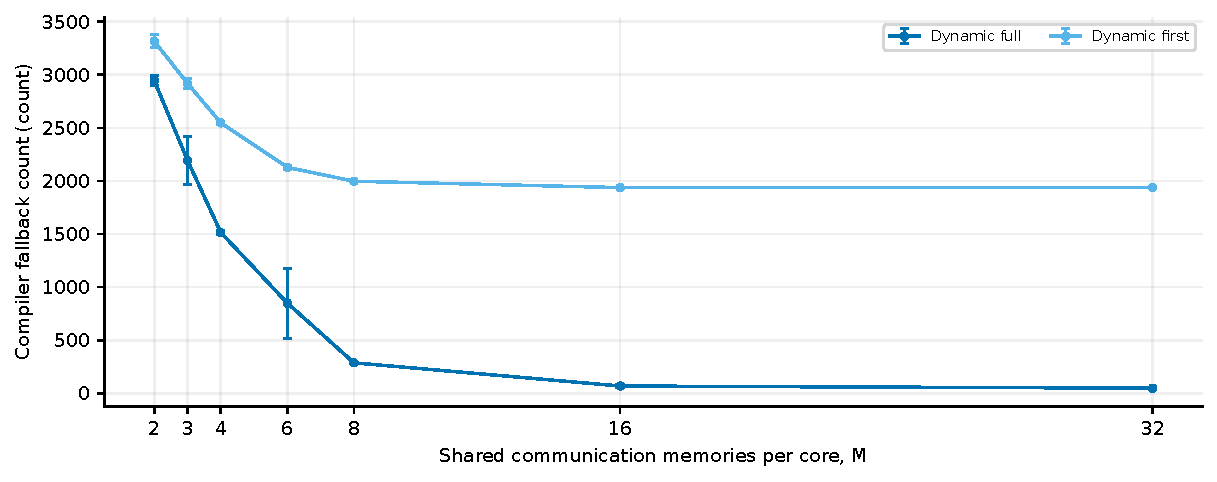
\includegraphics[width=.94\linewidth,height=.255\textheight,keepaspectratio]{figures/memory/mesh_xy_on_demand_fallbacks.pdf}\captionof{figure}{Run-level mean and sample SD. Shared trace aliases are counted once.}\end{center}
\begin{center}{\scriptsize\setlength{\tabcolsep}{3pt}
\begin{tabular}{lrrrrr}
\toprule
M & ODG & CGP & ACGP & Dynamic full & Dynamic first \\
\midrule
2 & n/a & n/a & n/a & $2945.00\pm46.67$ & $3315.50\pm60.10$ \\
3 & n/a & n/a & n/a & $2193.00\pm226.27$ & $2918.00\pm46.67$ \\
4 & n/a & n/a & n/a & $1514.00\pm16.97$ & $2547.00\pm12.73$ \\
6 & n/a & n/a & n/a & $849.50\pm328.80$ & $2127.50\pm14.85$ \\
8 & n/a & n/a & n/a & $287.50\pm6.36$ & $1997.50\pm0.71$ \\
16 & n/a & n/a & n/a & $69.000\pm12.728$ & $1937.00\pm1.41$ \\
32 & n/a & n/a & n/a & $48.500\pm6.364$ & $1937.00\pm1.41$ \\
\bottomrule\end{tabular}}
\captionof{table}{Mean $\pm$ sample SD; n/a denotes a metric outside that policy's instrumentation.}
{\footnotesize\href{https://github.com/sanjeevkrishnaa/Compiler-Driven-ACE/blob/codex/ace-scheduler-correctness/docs/latex/qft96_final/data/memory_mesh_xy_on_demand_fallbacks.csv}{Exact CSV values and sample counts}}
\end{center}
\clearpage
\subsection*{Generated compiler pairs}
\begin{center}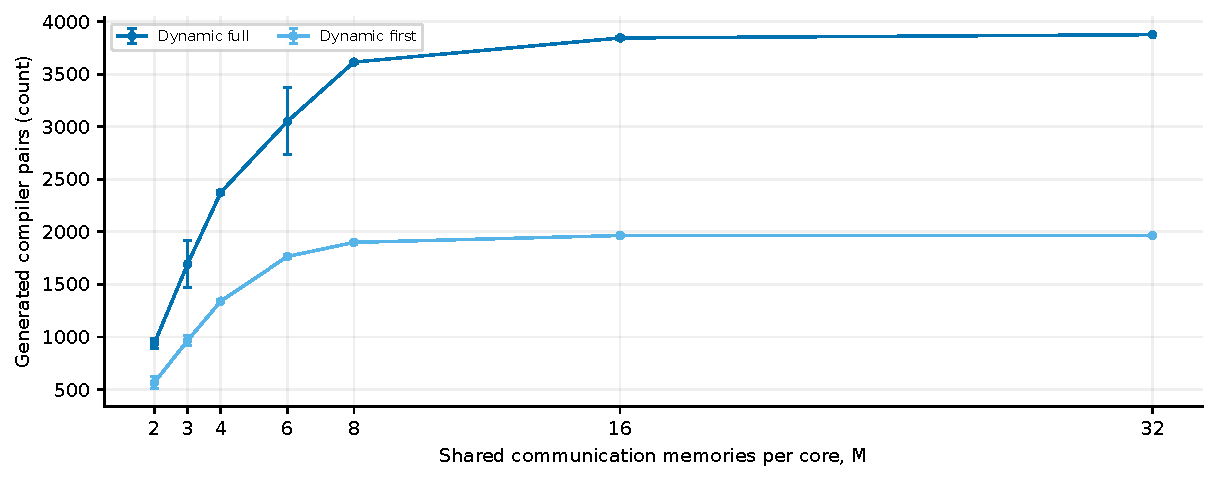
\includegraphics[width=.94\linewidth,height=.255\textheight,keepaspectratio]{figures/memory/mesh_xy_generated_compiler_pairs.pdf}\captionof{figure}{Run-level mean and sample SD. Shared trace aliases are counted once.}\end{center}
\begin{center}{\scriptsize\setlength{\tabcolsep}{3pt}
\begin{tabular}{lrrrrr}
\toprule
M & ODG & CGP & ACGP & Dynamic full & Dynamic first \\
\midrule
2 & n/a & n/a & n/a & $935.00\pm45.25$ & $564.50\pm58.69$ \\
3 & n/a & n/a & n/a & $1692.50\pm221.32$ & $965.50\pm44.55$ \\
4 & n/a & n/a & n/a & $2375.50\pm16.26$ & $1340.50\pm12.02$ \\
6 & n/a & n/a & n/a & $3050.50\pm318.91$ & $1765.00\pm18.38$ \\
8 & n/a & n/a & n/a & $3615.00\pm8.49$ & $1899.50\pm3.54$ \\
16 & n/a & n/a & n/a & $3844.50\pm10.61$ & $1965.00\pm0.00$ \\
32 & n/a & n/a & n/a & $3876.00\pm0.00$ & $1965.00\pm0.00$ \\
\bottomrule\end{tabular}}
\captionof{table}{Mean $\pm$ sample SD; n/a denotes a metric outside that policy's instrumentation.}
{\footnotesize\href{https://github.com/sanjeevkrishnaa/Compiler-Driven-ACE/blob/codex/ace-scheduler-correctness/docs/latex/qft96_final/data/memory_mesh_xy_generated_compiler_pairs.csv}{Exact CSV values and sample counts}}
\end{center}
\subsection*{Used compiler pairs}
\begin{center}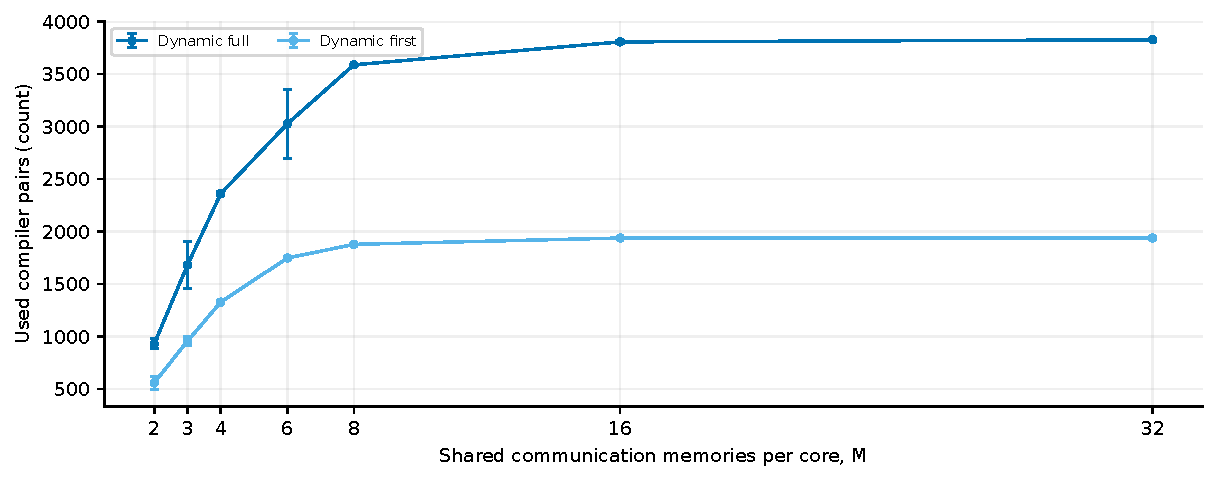
\includegraphics[width=.94\linewidth,height=.255\textheight,keepaspectratio]{figures/memory/mesh_xy_utilized_compiler_pairs.pdf}\captionof{figure}{Run-level mean and sample SD. Shared trace aliases are counted once.}\end{center}
\begin{center}{\scriptsize\setlength{\tabcolsep}{3pt}
\begin{tabular}{lrrrrr}
\toprule
M & ODG & CGP & ACGP & Dynamic full & Dynamic first \\
\midrule
2 & n/a & n/a & n/a & $931.00\pm46.67$ & $560.50\pm60.10$ \\
3 & n/a & n/a & n/a & $1683.00\pm226.27$ & $958.00\pm46.67$ \\
4 & n/a & n/a & n/a & $2362.00\pm16.97$ & $1329.00\pm12.73$ \\
6 & n/a & n/a & n/a & $3026.50\pm328.80$ & $1748.50\pm14.85$ \\
8 & n/a & n/a & n/a & $3588.50\pm6.36$ & $1878.50\pm0.71$ \\
16 & n/a & n/a & n/a & $3807.00\pm12.73$ & $1939.00\pm1.41$ \\
32 & n/a & n/a & n/a & $3827.50\pm6.36$ & $1939.00\pm1.41$ \\
\bottomrule\end{tabular}}
\captionof{table}{Mean $\pm$ sample SD; n/a denotes a metric outside that policy's instrumentation.}
{\footnotesize\href{https://github.com/sanjeevkrishnaa/Compiler-Driven-ACE/blob/codex/ace-scheduler-correctness/docs/latex/qft96_final/data/memory_mesh_xy_utilized_compiler_pairs.csv}{Exact CSV values and sample counts}}
\end{center}
\clearpage
\subsection*{Expired compiler pairs}
\begin{center}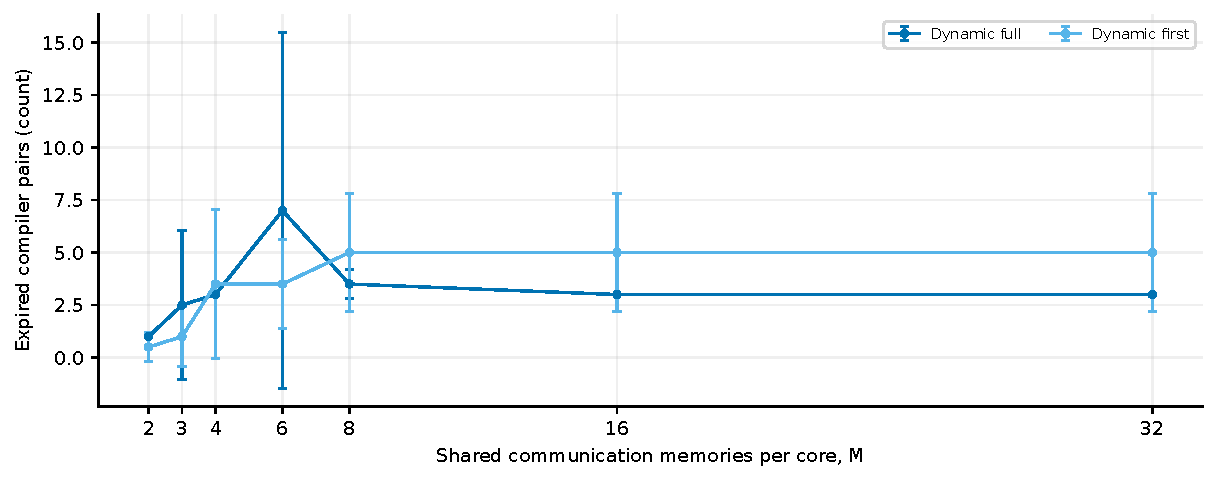
\includegraphics[width=.94\linewidth,height=.255\textheight,keepaspectratio]{figures/memory/mesh_xy_expired_compiler_pairs.pdf}\captionof{figure}{Run-level mean and sample SD. Shared trace aliases are counted once.}\end{center}
\begin{center}{\scriptsize\setlength{\tabcolsep}{3pt}
\begin{tabular}{lrrrrr}
\toprule
M & ODG & CGP & ACGP & Dynamic full & Dynamic first \\
\midrule
2 & n/a & n/a & n/a & $1.000\pm0.000$ & $0.5000\pm0.7071$ \\
3 & n/a & n/a & n/a & $2.500\pm3.536$ & $1.000\pm1.414$ \\
4 & n/a & n/a & n/a & $3.000\pm0.000$ & $3.500\pm3.536$ \\
6 & n/a & n/a & n/a & $7.000\pm8.485$ & $3.500\pm2.121$ \\
8 & n/a & n/a & n/a & $3.500\pm0.707$ & $5.000\pm2.828$ \\
16 & n/a & n/a & n/a & $3.000\pm0.000$ & $5.000\pm2.828$ \\
32 & n/a & n/a & n/a & $3.000\pm0.000$ & $5.000\pm2.828$ \\
\bottomrule\end{tabular}}
\captionof{table}{Mean $\pm$ sample SD; n/a denotes a metric outside that policy's instrumentation.}
{\footnotesize\href{https://github.com/sanjeevkrishnaa/Compiler-Driven-ACE/blob/codex/ace-scheduler-correctness/docs/latex/qft96_final/data/memory_mesh_xy_expired_compiler_pairs.csv}{Exact CSV values and sample counts}}
\end{center}
\subsection*{Remaining compiler pairs}
\begin{center}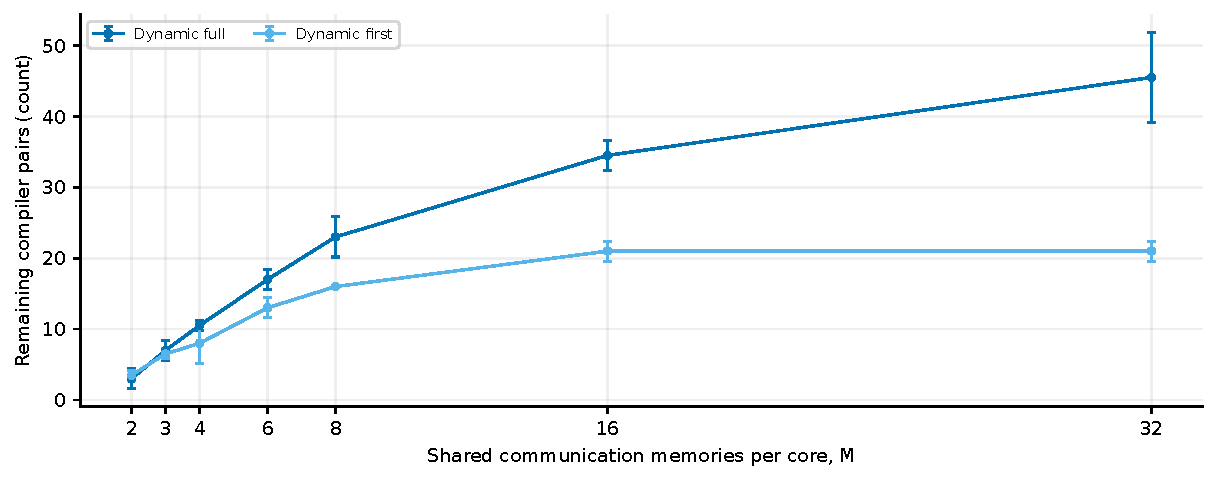
\includegraphics[width=.94\linewidth,height=.255\textheight,keepaspectratio]{figures/memory/mesh_xy_remaining_compiler_pairs.pdf}\captionof{figure}{Run-level mean and sample SD. Shared trace aliases are counted once.}\end{center}
\begin{center}{\scriptsize\setlength{\tabcolsep}{3pt}
\begin{tabular}{lrrrrr}
\toprule
M & ODG & CGP & ACGP & Dynamic full & Dynamic first \\
\midrule
2 & n/a & n/a & n/a & $3.000\pm1.414$ & $3.500\pm0.707$ \\
3 & n/a & n/a & n/a & $7.000\pm1.414$ & $6.500\pm0.707$ \\
4 & n/a & n/a & n/a & $10.500\pm0.707$ & $8.000\pm2.828$ \\
6 & n/a & n/a & n/a & $17.000\pm1.414$ & $13.000\pm1.414$ \\
8 & n/a & n/a & n/a & $23.000\pm2.828$ & $16.000\pm0.000$ \\
16 & n/a & n/a & n/a & $34.500\pm2.121$ & $21.000\pm1.414$ \\
32 & n/a & n/a & n/a & $45.500\pm6.364$ & $21.000\pm1.414$ \\
\bottomrule\end{tabular}}
\captionof{table}{Mean $\pm$ sample SD; n/a denotes a metric outside that policy's instrumentation.}
{\footnotesize\href{https://github.com/sanjeevkrishnaa/Compiler-Driven-ACE/blob/codex/ace-scheduler-correctness/docs/latex/qft96_final/data/memory_mesh_xy_remaining_compiler_pairs.csv}{Exact CSV values and sample counts}}
\end{center}
\clearpage
\subsection*{Compiler fidelity at creation}
\begin{center}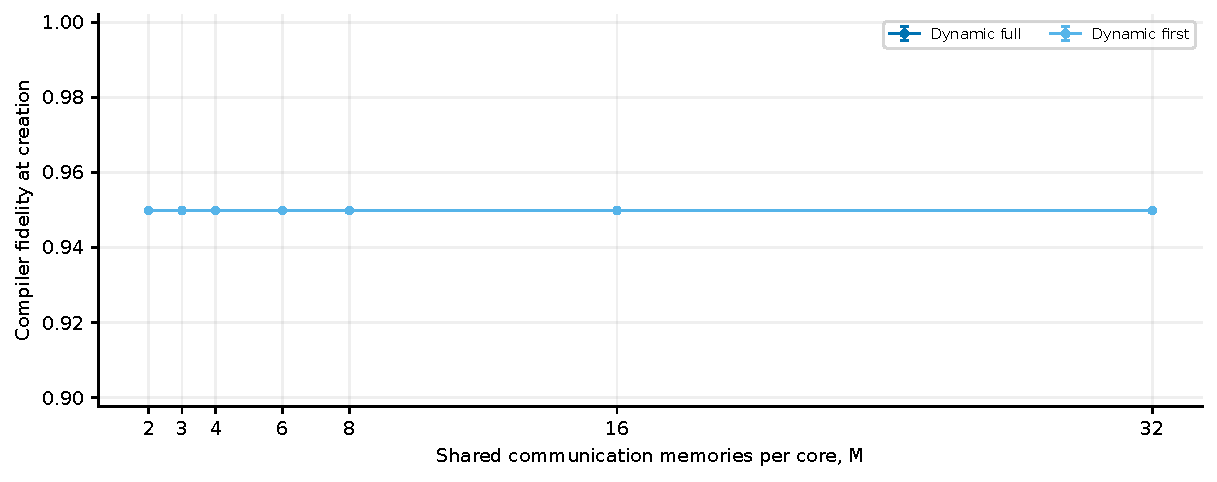
\includegraphics[width=.94\linewidth,height=.255\textheight,keepaspectratio]{figures/memory/mesh_xy_average_fidelity_at_creation.pdf}\captionof{figure}{Run-level mean and sample SD. Shared trace aliases are counted once.}\end{center}
\begin{center}{\scriptsize\setlength{\tabcolsep}{3pt}
\begin{tabular}{lrrrrr}
\toprule
M & ODG & CGP & ACGP & Dynamic full & Dynamic first \\
\midrule
2 & n/a & n/a & n/a & $0.9498\pm0.0000$ & $0.9498\pm0.0000$ \\
3 & n/a & n/a & n/a & $0.9498\pm0.0000$ & $0.9498\pm0.0000$ \\
4 & n/a & n/a & n/a & $0.9498\pm0.0000$ & $0.9498\pm0.0000$ \\
6 & n/a & n/a & n/a & $0.9498\pm0.0000$ & $0.9498\pm0.0000$ \\
8 & n/a & n/a & n/a & $0.9498\pm0.0000$ & $0.9498\pm0.0000$ \\
16 & n/a & n/a & n/a & $0.9498\pm0.0000$ & $0.9498\pm0.0000$ \\
32 & n/a & n/a & n/a & $0.9498\pm0.0000$ & $0.9498\pm0.0000$ \\
\bottomrule\end{tabular}}
\captionof{table}{Mean $\pm$ sample SD; n/a denotes a metric outside that policy's instrumentation.}
{\footnotesize\href{https://github.com/sanjeevkrishnaa/Compiler-Driven-ACE/blob/codex/ace-scheduler-correctness/docs/latex/qft96_final/data/memory_mesh_xy_average_fidelity_at_creation.csv}{Exact CSV values and sample counts}}
\end{center}
\subsection*{Compiler fidelity at use}
\begin{center}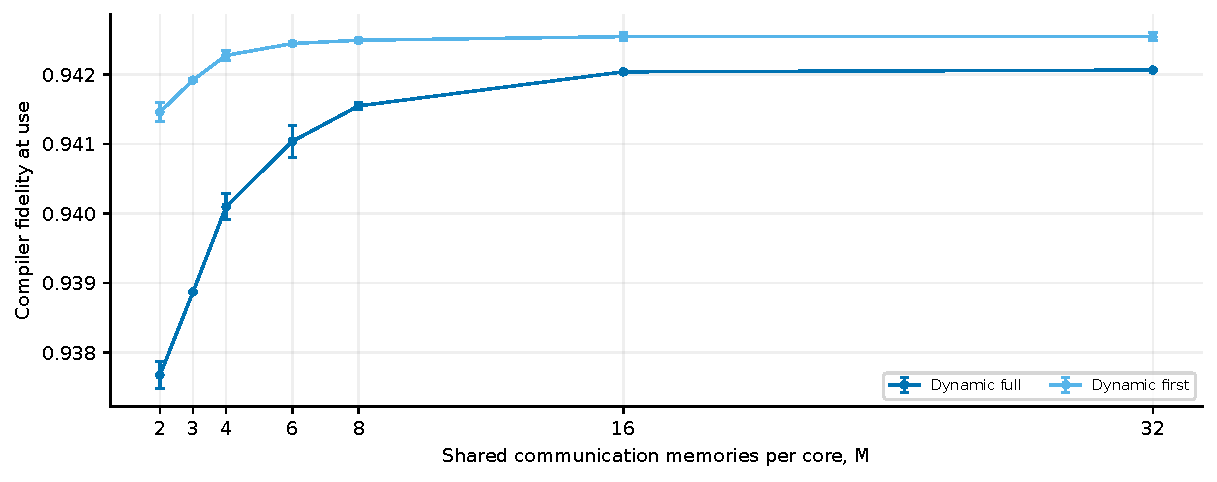
\includegraphics[width=.94\linewidth,height=.255\textheight,keepaspectratio]{figures/memory/mesh_xy_average_fidelity_at_utilization.pdf}\captionof{figure}{Run-level mean and sample SD. Shared trace aliases are counted once.}\end{center}
\begin{center}{\scriptsize\setlength{\tabcolsep}{3pt}
\begin{tabular}{lrrrrr}
\toprule
M & ODG & CGP & ACGP & Dynamic full & Dynamic first \\
\midrule
2 & n/a & n/a & n/a & $0.9377\pm0.0002$ & $0.9415\pm0.0001$ \\
3 & n/a & n/a & n/a & $0.9389\pm0.0000$ & $0.9419\pm0.0000$ \\
4 & n/a & n/a & n/a & $0.9401\pm0.0002$ & $0.9423\pm0.0001$ \\
6 & n/a & n/a & n/a & $0.9410\pm0.0002$ & $0.9424\pm0.0000$ \\
8 & n/a & n/a & n/a & $0.9415\pm0.0000$ & $0.9425\pm0.0000$ \\
16 & n/a & n/a & n/a & $0.9420\pm0.0000$ & $0.9425\pm0.0001$ \\
32 & n/a & n/a & n/a & $0.9421\pm0.0000$ & $0.9425\pm0.0001$ \\
\bottomrule\end{tabular}}
\captionof{table}{Mean $\pm$ sample SD; n/a denotes a metric outside that policy's instrumentation.}
{\footnotesize\href{https://github.com/sanjeevkrishnaa/Compiler-Driven-ACE/blob/codex/ace-scheduler-correctness/docs/latex/qft96_final/data/memory_mesh_xy_average_fidelity_at_utilization.csv}{Exact CSV values and sample counts}}
\end{center}
\clearpage
\subsection*{Mean layer latency}
\begin{center}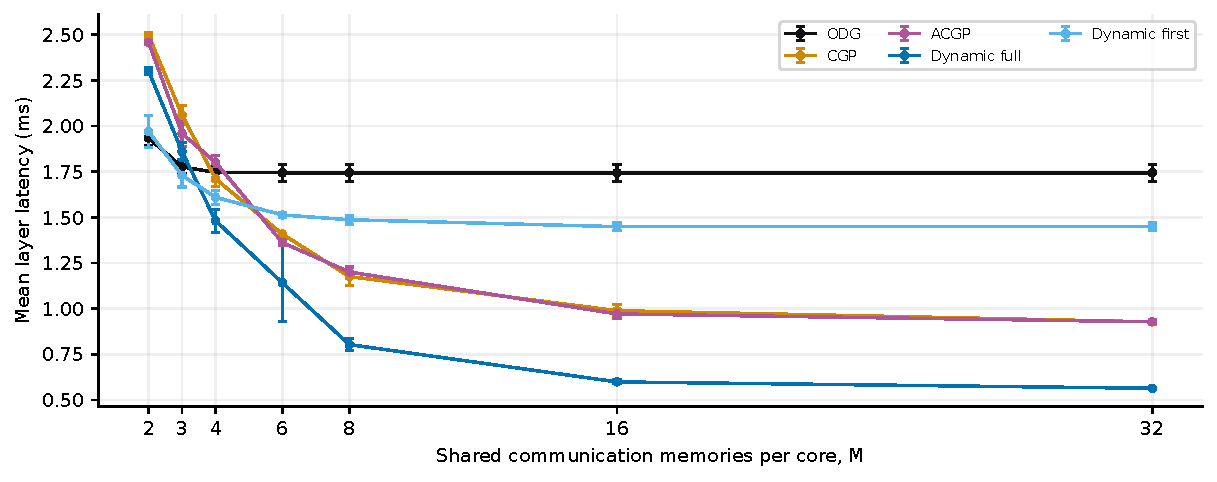
\includegraphics[width=.94\linewidth,height=.255\textheight,keepaspectratio]{figures/memory/mesh_xy_avg_layer_latency_ms.pdf}\captionof{figure}{Run-level mean and sample SD. Shared trace aliases are counted once.}\end{center}
\begin{center}{\scriptsize\setlength{\tabcolsep}{3pt}
\begin{tabular}{lrrrrr}
\toprule
M & ODG & CGP & ACGP & Dynamic full & Dynamic first \\
\midrule
2 & $1.935\pm0.040$ & $2.498\pm0.016$ & $2.458\pm0.010$ & $2.302\pm0.018$ & $1.971\pm0.088$ \\
3 & $1.777\pm0.034$ & $2.061\pm0.054$ & $1.959\pm0.071$ & $1.861\pm0.047$ & $1.731\pm0.064$ \\
4 & $1.746\pm0.040$ & $1.711\pm0.040$ & $1.802\pm0.036$ & $1.482\pm0.062$ & $1.610\pm0.038$ \\
6 & $1.744\pm0.047$ & $1.409\pm0.006$ & $1.362\pm0.017$ & $1.142\pm0.213$ & $1.514\pm0.012$ \\
8 & $1.744\pm0.047$ & $1.176\pm0.051$ & $1.201\pm0.028$ & $0.8035\pm0.0319$ & $1.487\pm0.025$ \\
16 & $1.744\pm0.047$ & $0.9892\pm0.0314$ & $0.9714\pm0.0233$ & $0.5992\pm0.0108$ & $1.449\pm0.020$ \\
32 & $1.744\pm0.047$ & $0.9280\pm0.0115$ & $0.9282\pm0.0099$ & $0.5641\pm0.0024$ & $1.449\pm0.020$ \\
\bottomrule\end{tabular}}
\captionof{table}{Mean $\pm$ sample SD; n/a denotes a metric outside that policy's instrumentation.}
{\footnotesize\href{https://github.com/sanjeevkrishnaa/Compiler-Driven-ACE/blob/codex/ace-scheduler-correctness/docs/latex/qft96_final/data/memory_mesh_xy_avg_layer_latency_ms.csv}{Exact CSV values and sample counts}}
\end{center}
\subsection*{Maximum layer latency}
\begin{center}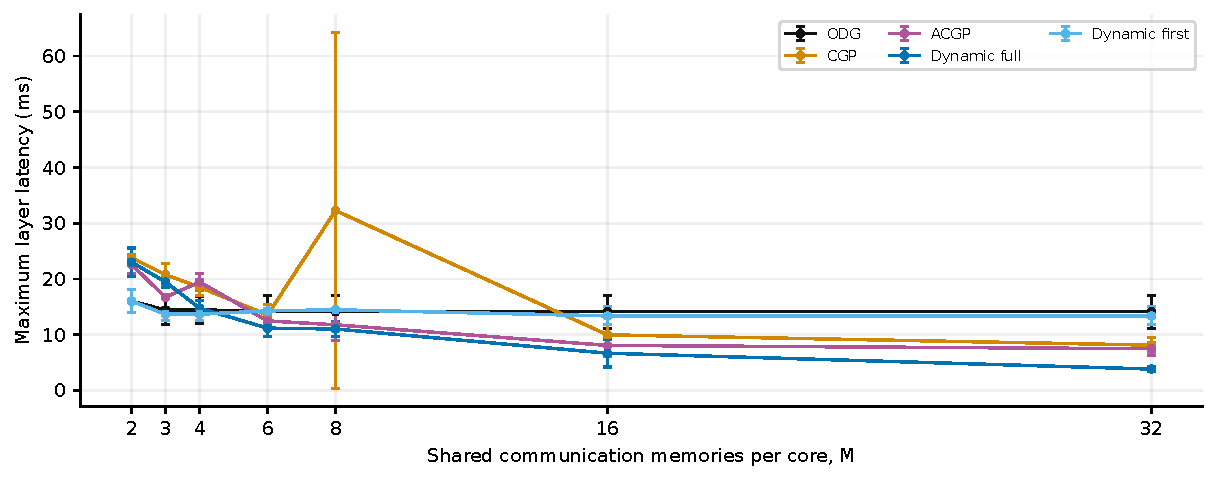
\includegraphics[width=.94\linewidth,height=.255\textheight,keepaspectratio]{figures/memory/mesh_xy_max_layer_latency_ms.pdf}\captionof{figure}{Run-level mean and sample SD. Shared trace aliases are counted once.}\end{center}
\begin{center}{\scriptsize\setlength{\tabcolsep}{3pt}
\begin{tabular}{lrrrrr}
\toprule
M & ODG & CGP & ACGP & Dynamic full & Dynamic first \\
\midrule
2 & $16.000\pm0.283$ & $23.801\pm0.566$ & $22.551\pm1.626$ & $23.001\pm2.546$ & $16.000\pm2.121$ \\
3 & $14.400\pm2.546$ & $20.750\pm2.051$ & $16.700\pm0.141$ & $19.450\pm0.919$ & $13.650\pm1.202$ \\
4 & $14.450\pm2.475$ & $18.518\pm1.439$ & $19.450\pm1.485$ & $14.750\pm1.344$ & $13.650\pm1.202$ \\
6 & $14.100\pm2.970$ & $13.500\pm1.980$ & $12.450\pm0.778$ & $11.150\pm1.485$ & $14.250\pm0.354$ \\
8 & $14.100\pm2.970$ & $32.271\pm32.003$ & $11.750\pm2.899$ & $11.000\pm1.273$ & $14.450\pm0.071$ \\
16 & $14.100\pm2.970$ & $9.950\pm3.748$ & $8.050\pm2.051$ & $6.650\pm2.475$ & $13.350\pm1.626$ \\
32 & $14.100\pm2.970$ & $8.100\pm1.414$ & $7.450\pm1.202$ & $3.800\pm0.424$ & $13.350\pm1.626$ \\
\bottomrule\end{tabular}}
\captionof{table}{Mean $\pm$ sample SD; n/a denotes a metric outside that policy's instrumentation.}
{\footnotesize\href{https://github.com/sanjeevkrishnaa/Compiler-Driven-ACE/blob/codex/ace-scheduler-correctness/docs/latex/qft96_final/data/memory_mesh_xy_max_layer_latency_ms.csv}{Exact CSV values and sample counts}}
\end{center}
\clearpage
\subsection*{Minimum layer latency}
\begin{center}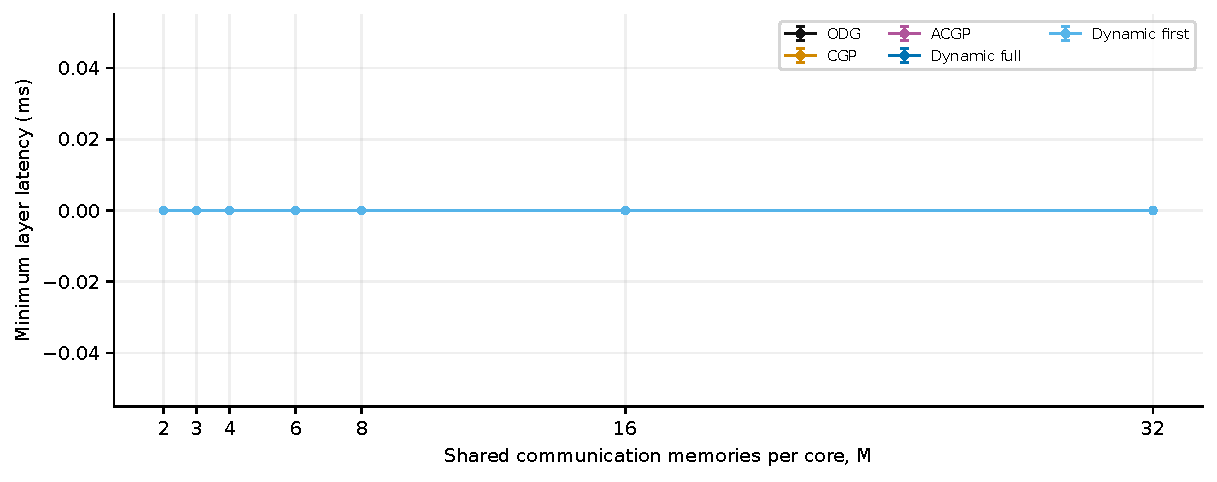
\includegraphics[width=.94\linewidth,height=.255\textheight,keepaspectratio]{figures/memory/mesh_xy_min_layer_latency_ms.pdf}\captionof{figure}{Run-level mean and sample SD. Shared trace aliases are counted once.}\end{center}
\begin{center}{\scriptsize\setlength{\tabcolsep}{3pt}
\begin{tabular}{lrrrrr}
\toprule
M & ODG & CGP & ACGP & Dynamic full & Dynamic first \\
\midrule
2 & $0.0000\pm0.0000$ & $0.0000\pm0.0000$ & $0.0000\pm0.0000$ & $0.0000\pm0.0000$ & $0.0000\pm0.0000$ \\
3 & $0.0000\pm0.0000$ & $0.0000\pm0.0000$ & $0.0000\pm0.0000$ & $0.0000\pm0.0000$ & $0.0000\pm0.0000$ \\
4 & $0.0000\pm0.0000$ & $0.0000\pm0.0000$ & $0.0000\pm0.0000$ & $0.0000\pm0.0000$ & $0.0000\pm0.0000$ \\
6 & $0.0000\pm0.0000$ & $0.0000\pm0.0000$ & $0.0000\pm0.0000$ & $0.0000\pm0.0000$ & $0.0000\pm0.0000$ \\
8 & $0.0000\pm0.0000$ & $0.0000\pm0.0000$ & $0.0000\pm0.0000$ & $0.0000\pm0.0000$ & $0.0000\pm0.0000$ \\
16 & $0.0000\pm0.0000$ & $0.0000\pm0.0000$ & $0.0000\pm0.0000$ & $0.0000\pm0.0000$ & $0.0000\pm0.0000$ \\
32 & $0.0000\pm0.0000$ & $0.0000\pm0.0000$ & $0.0000\pm0.0000$ & $0.0000\pm0.0000$ & $0.0000\pm0.0000$ \\
\bottomrule\end{tabular}}
\captionof{table}{Mean $\pm$ sample SD; n/a denotes a metric outside that policy's instrumentation.}
{\footnotesize\href{https://github.com/sanjeevkrishnaa/Compiler-Driven-ACE/blob/codex/ace-scheduler-correctness/docs/latex/qft96_final/data/memory_mesh_xy_min_layer_latency_ms.csv}{Exact CSV values and sample counts}}
\end{center}
\section{YX}
\clearpage
\subsection*{Mean request latency}
\begin{center}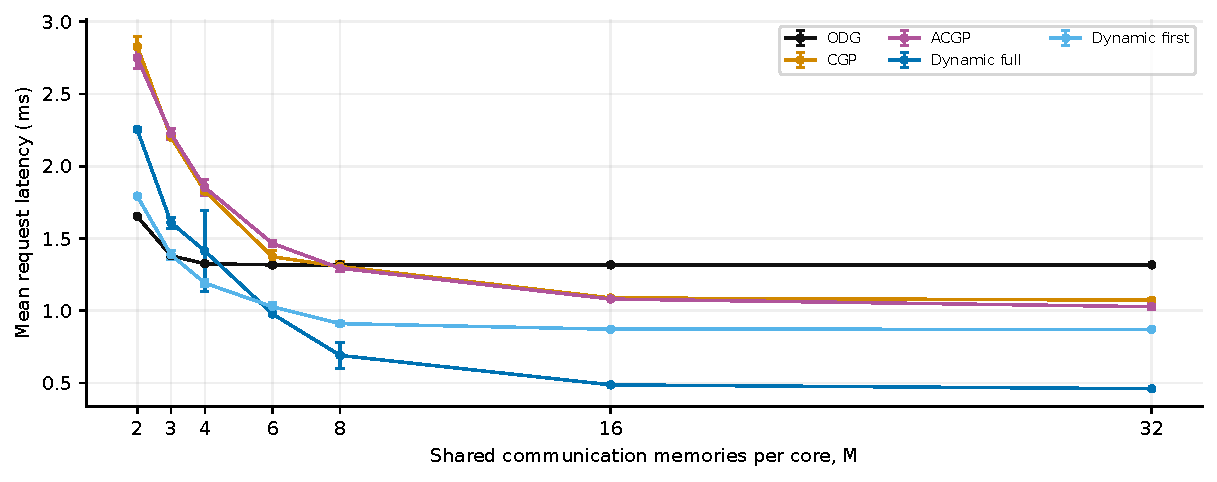
\includegraphics[width=.94\linewidth,height=.255\textheight,keepaspectratio]{figures/memory/mesh_yx_request_latency_mean_ms.pdf}\captionof{figure}{Run-level mean and sample SD. Shared trace aliases are counted once.}\end{center}
\begin{center}{\scriptsize\setlength{\tabcolsep}{3pt}
\begin{tabular}{lrrrrr}
\toprule
M & ODG & CGP & ACGP & Dynamic full & Dynamic first \\
\midrule
2 & $1.653\pm0.005$ & $2.827\pm0.069$ & $2.751\pm0.076$ & $2.254\pm0.014$ & $1.793\pm0.008$ \\
3 & $1.381\pm0.005$ & $2.202\pm0.010$ & $2.224\pm0.040$ & $1.610\pm0.038$ & $1.387\pm0.033$ \\
4 & $1.326\pm0.001$ & $1.828\pm0.019$ & $1.854\pm0.055$ & $1.414\pm0.282$ & $1.192\pm0.025$ \\
6 & $1.318\pm0.000$ & $1.374\pm0.044$ & $1.466\pm0.019$ & $0.9785\pm0.0017$ & $1.029\pm0.030$ \\
8 & $1.318\pm0.000$ & $1.307\pm0.037$ & $1.295\pm0.026$ & $0.6916\pm0.0885$ & $0.9115\pm0.0118$ \\
16 & $1.318\pm0.000$ & $1.089\pm0.001$ & $1.081\pm0.005$ & $0.4880\pm0.0003$ & $0.8725\pm0.0012$ \\
32 & $1.318\pm0.000$ & $1.073\pm0.012$ & $1.028\pm0.019$ & $0.4607\pm0.0012$ & $0.8724\pm0.0011$ \\
\bottomrule\end{tabular}}
\captionof{table}{Mean $\pm$ sample SD; n/a denotes a metric outside that policy's instrumentation.}
{\footnotesize\href{https://github.com/sanjeevkrishnaa/Compiler-Driven-ACE/blob/codex/ace-scheduler-correctness/docs/latex/qft96_final/data/memory_mesh_yx_request_latency_mean_ms.csv}{Exact CSV values and sample counts}}
\end{center}
\subsection*{Median request latency}
\begin{center}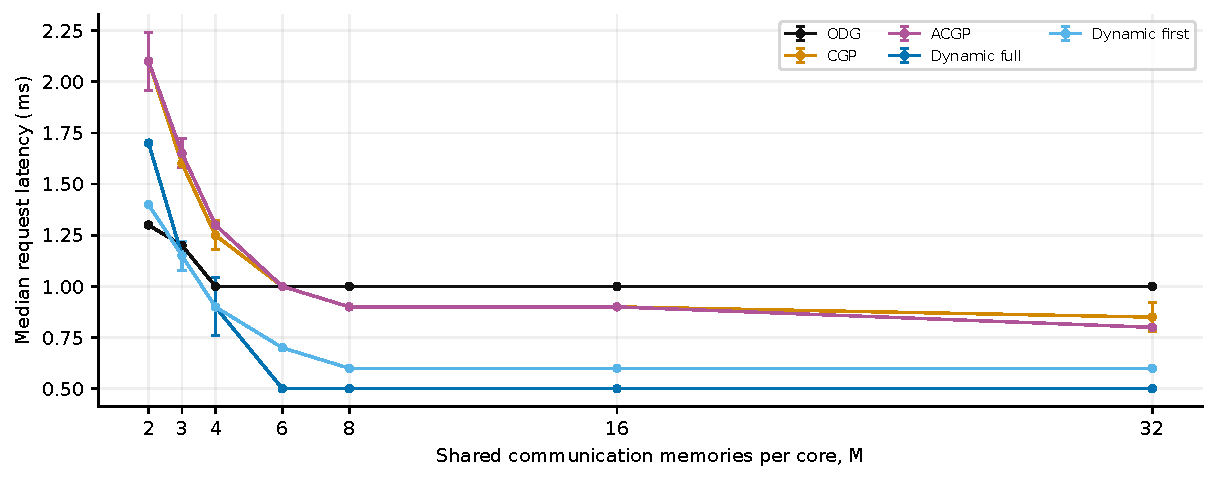
\includegraphics[width=.94\linewidth,height=.255\textheight,keepaspectratio]{figures/memory/mesh_yx_request_latency_median_ms.pdf}\captionof{figure}{Run-level mean and sample SD. Shared trace aliases are counted once.}\end{center}
\begin{center}{\scriptsize\setlength{\tabcolsep}{3pt}
\begin{tabular}{lrrrrr}
\toprule
M & ODG & CGP & ACGP & Dynamic full & Dynamic first \\
\midrule
2 & $1.300\pm0.000$ & $2.100\pm0.000$ & $2.100\pm0.141$ & $1.700\pm0.000$ & $1.400\pm0.000$ \\
3 & $1.200\pm0.000$ & $1.600\pm0.000$ & $1.650\pm0.071$ & $1.150\pm0.071$ & $1.150\pm0.071$ \\
4 & $1.000\pm0.000$ & $1.250\pm0.071$ & $1.300\pm0.000$ & $0.9000\pm0.1414$ & $0.9000\pm0.0000$ \\
6 & $1.000\pm0.000$ & $1.000\pm0.000$ & $1.000\pm0.000$ & $0.5000\pm0.0000$ & $0.7000\pm0.0000$ \\
8 & $1.000\pm0.000$ & $0.9000\pm0.0000$ & $0.9000\pm0.0000$ & $0.5000\pm0.0000$ & $0.6000\pm0.0000$ \\
16 & $1.000\pm0.000$ & $0.9000\pm0.0000$ & $0.9000\pm0.0000$ & $0.5000\pm0.0000$ & $0.6000\pm0.0000$ \\
32 & $1.000\pm0.000$ & $0.8500\pm0.0707$ & $0.8000\pm0.0000$ & $0.5000\pm0.0000$ & $0.6000\pm0.0000$ \\
\bottomrule\end{tabular}}
\captionof{table}{Mean $\pm$ sample SD; n/a denotes a metric outside that policy's instrumentation.}
{\footnotesize\href{https://github.com/sanjeevkrishnaa/Compiler-Driven-ACE/blob/codex/ace-scheduler-correctness/docs/latex/qft96_final/data/memory_mesh_yx_request_latency_median_ms.csv}{Exact CSV values and sample counts}}
\end{center}
\clearpage
\subsection*{p95 request latency}
\begin{center}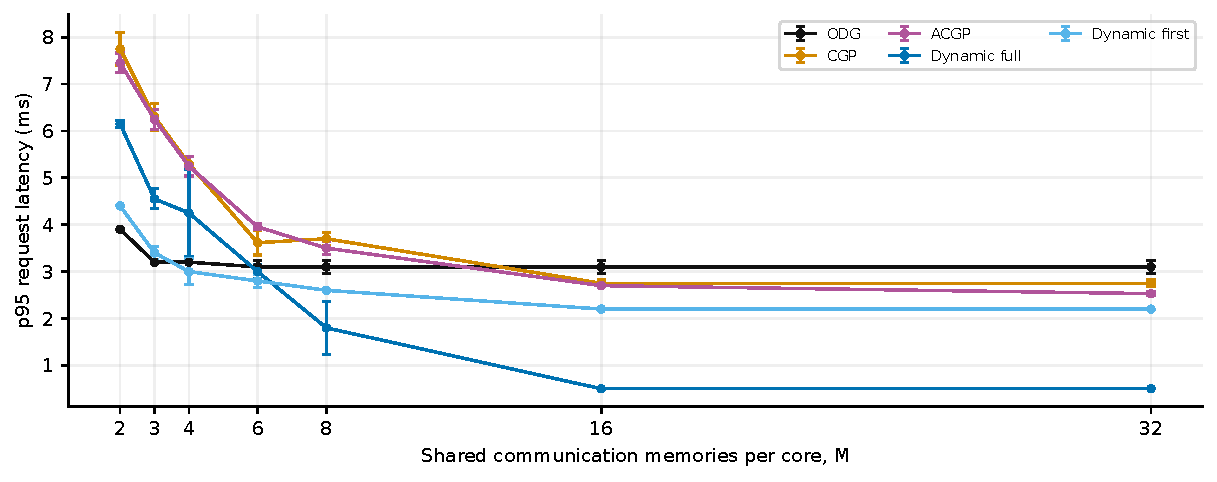
\includegraphics[width=.94\linewidth,height=.255\textheight,keepaspectratio]{figures/memory/mesh_yx_request_latency_p95_ms.pdf}\captionof{figure}{Run-level mean and sample SD. Shared trace aliases are counted once.}\end{center}
\begin{center}{\scriptsize\setlength{\tabcolsep}{3pt}
\begin{tabular}{lrrrrr}
\toprule
M & ODG & CGP & ACGP & Dynamic full & Dynamic first \\
\midrule
2 & $3.900\pm0.000$ & $7.750\pm0.354$ & $7.450\pm0.212$ & $6.150\pm0.071$ & $4.400\pm0.000$ \\
3 & $3.200\pm0.000$ & $6.300\pm0.283$ & $6.250\pm0.212$ & $4.550\pm0.212$ & $3.400\pm0.141$ \\
4 & $3.200\pm0.000$ & $5.300\pm0.000$ & $5.250\pm0.212$ & $4.250\pm0.919$ & $3.000\pm0.283$ \\
6 & $3.100\pm0.141$ & $3.615\pm0.262$ & $3.955\pm0.064$ & $3.000\pm0.141$ & $2.800\pm0.141$ \\
8 & $3.100\pm0.141$ & $3.700\pm0.141$ & $3.500\pm0.141$ & $1.800\pm0.566$ & $2.600\pm0.000$ \\
16 & $3.100\pm0.141$ & $2.750\pm0.071$ & $2.700\pm0.000$ & $0.5000\pm0.0000$ & $2.200\pm0.000$ \\
32 & $3.100\pm0.141$ & $2.750\pm0.071$ & $2.529\pm0.036$ & $0.5000\pm0.0000$ & $2.200\pm0.000$ \\
\bottomrule\end{tabular}}
\captionof{table}{Mean $\pm$ sample SD; n/a denotes a metric outside that policy's instrumentation.}
{\footnotesize\href{https://github.com/sanjeevkrishnaa/Compiler-Driven-ACE/blob/codex/ace-scheduler-correctness/docs/latex/qft96_final/data/memory_mesh_yx_request_latency_p95_ms.csv}{Exact CSV values and sample counts}}
\end{center}
\subsection*{Maximum request latency}
\begin{center}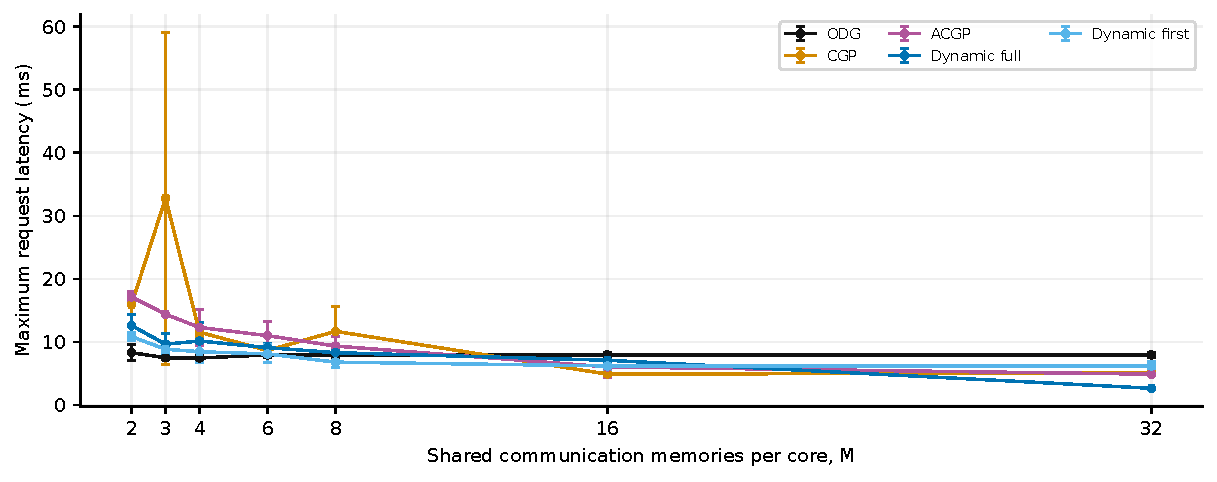
\includegraphics[width=.94\linewidth,height=.255\textheight,keepaspectratio]{figures/memory/mesh_yx_request_latency_max_ms.pdf}\captionof{figure}{Run-level mean and sample SD. Shared trace aliases are counted once.}\end{center}
\begin{center}{\scriptsize\setlength{\tabcolsep}{3pt}
\begin{tabular}{lrrrrr}
\toprule
M & ODG & CGP & ACGP & Dynamic full & Dynamic first \\
\midrule
2 & $8.300\pm1.273$ & $15.900\pm1.556$ & $17.150\pm0.778$ & $12.600\pm1.697$ & $10.850\pm0.636$ \\
3 & $7.500\pm0.283$ & $32.800\pm26.304$ & $14.400\pm0.141$ & $9.650\pm1.626$ & $8.850\pm0.495$ \\
4 & $7.450\pm0.354$ & $11.550\pm0.636$ & $12.300\pm2.828$ & $10.150\pm2.899$ & $8.450\pm1.626$ \\
6 & $7.950\pm0.354$ & $8.650\pm0.778$ & $11.000\pm2.263$ & $9.100\pm0.707$ & $8.100\pm1.414$ \\
8 & $7.950\pm0.354$ & $11.682\pm3.986$ & $9.350\pm1.485$ & $8.300\pm0.283$ & $6.800\pm0.849$ \\
16 & $7.950\pm0.354$ & $4.900\pm0.000$ & $6.043\pm1.616$ & $7.100\pm0.566$ & $6.200\pm0.707$ \\
32 & $7.950\pm0.354$ & $5.096\pm0.277$ & $4.889\pm0.016$ & $2.650\pm0.071$ & $6.200\pm0.707$ \\
\bottomrule\end{tabular}}
\captionof{table}{Mean $\pm$ sample SD; n/a denotes a metric outside that policy's instrumentation.}
{\footnotesize\href{https://github.com/sanjeevkrishnaa/Compiler-Driven-ACE/blob/codex/ace-scheduler-correctness/docs/latex/qft96_final/data/memory_mesh_yx_request_latency_max_ms.csv}{Exact CSV values and sample counts}}
\end{center}
\clearpage
\subsection*{Communication makespan}
\begin{center}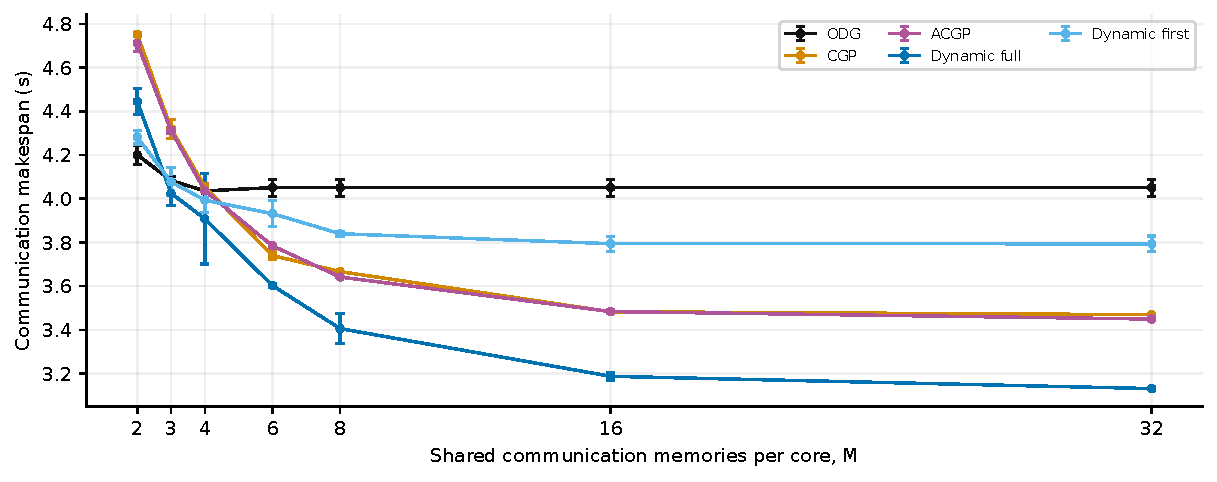
\includegraphics[width=.94\linewidth,height=.255\textheight,keepaspectratio]{figures/memory/mesh_yx_end_to_end_latency_ms.pdf}\captionof{figure}{Run-level mean and sample SD. Shared trace aliases are counted once.}\end{center}
\begin{center}{\scriptsize\setlength{\tabcolsep}{3pt}
\begin{tabular}{lrrrrr}
\toprule
M & ODG & CGP & ACGP & Dynamic full & Dynamic first \\
\midrule
2 & $4.201\pm0.044$ & $4.752\pm0.009$ & $4.711\pm0.036$ & $4.445\pm0.058$ & $4.282\pm0.032$ \\
3 & $4.083\pm0.017$ & $4.321\pm0.044$ & $4.312\pm0.013$ & $4.025\pm0.055$ & $4.077\pm0.064$ \\
4 & $4.036\pm0.032$ & $4.055\pm0.006$ & $4.037\pm0.032$ & $3.908\pm0.207$ & $3.993\pm0.058$ \\
6 & $4.051\pm0.039$ & $3.740\pm0.018$ & $3.784\pm0.006$ & $3.603\pm0.008$ & $3.932\pm0.060$ \\
8 & $4.051\pm0.039$ & $3.666\pm0.002$ & $3.642\pm0.004$ & $3.406\pm0.070$ & $3.840\pm0.011$ \\
16 & $4.051\pm0.039$ & $3.483\pm0.001$ & $3.484\pm0.008$ & $3.187\pm0.017$ & $3.794\pm0.035$ \\
32 & $4.051\pm0.039$ & $3.469\pm0.006$ & $3.449\pm0.007$ & $3.131\pm0.001$ & $3.794\pm0.035$ \\
\bottomrule\end{tabular}}
\captionof{table}{Mean $\pm$ sample SD; n/a denotes a metric outside that policy's instrumentation.}
{\footnotesize\href{https://github.com/sanjeevkrishnaa/Compiler-Driven-ACE/blob/codex/ace-scheduler-correctness/docs/latex/qft96_final/data/memory_mesh_yx_end_to_end_latency_ms.csv}{Exact CSV values and sample counts}}
\end{center}
\subsection*{Mean admission wait}
\begin{center}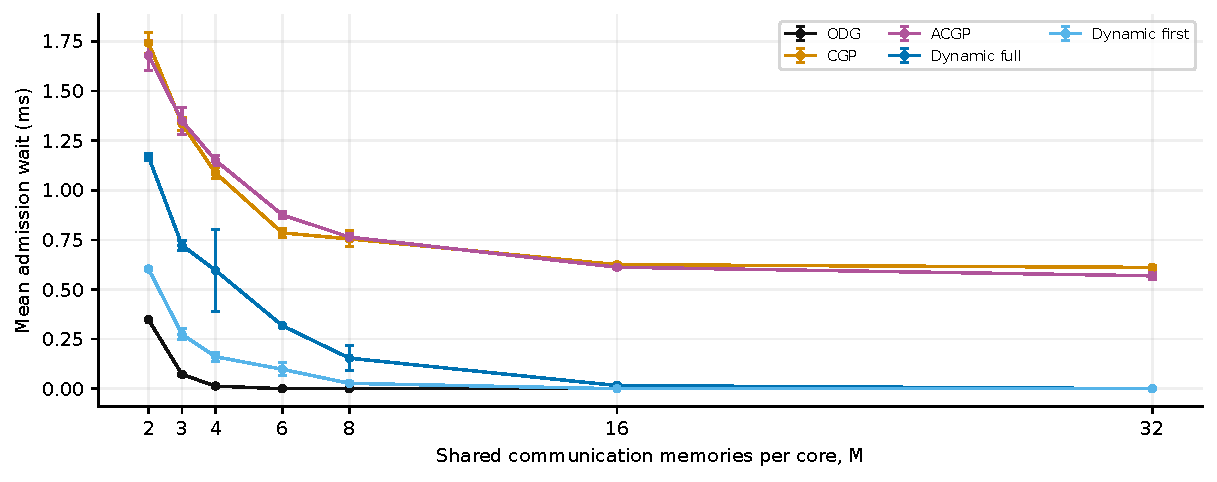
\includegraphics[width=.94\linewidth,height=.255\textheight,keepaspectratio]{figures/memory/mesh_yx_average_admission_wait_ms.pdf}\captionof{figure}{Run-level mean and sample SD. Shared trace aliases are counted once.}\end{center}
\begin{center}{\scriptsize\setlength{\tabcolsep}{3pt}
\begin{tabular}{lrrrrr}
\toprule
M & ODG & CGP & ACGP & Dynamic full & Dynamic first \\
\midrule
2 & $0.3471\pm0.0048$ & $1.742\pm0.054$ & $1.679\pm0.077$ & $1.167\pm0.016$ & $0.6028\pm0.0088$ \\
3 & $0.0722\pm0.0055$ & $1.334\pm0.033$ & $1.349\pm0.069$ & $0.7224\pm0.0258$ & $0.2747\pm0.0290$ \\
4 & $0.0133\pm0.0009$ & $1.087\pm0.029$ & $1.151\pm0.026$ & $0.5966\pm0.2069$ & $0.1613\pm0.0227$ \\
6 & $0.0000\pm0.0000$ & $0.7850\pm0.0223$ & $0.8758\pm0.0180$ & $0.3175\pm0.0065$ & $0.0979\pm0.0325$ \\
8 & $0.0000\pm0.0000$ & $0.7549\pm0.0405$ & $0.7639\pm0.0186$ & $0.1541\pm0.0621$ & $0.0272\pm0.0076$ \\
16 & $0.0000\pm0.0000$ & $0.6250\pm0.0060$ & $0.6123\pm0.0040$ & $0.0160\pm0.0051$ & $0.0001\pm0.0001$ \\
32 & $0.0000\pm0.0000$ & $0.6112\pm0.0119$ & $0.5687\pm0.0190$ & $0.0001\pm0.0002$ & $0.0000\pm0.0000$ \\
\bottomrule\end{tabular}}
\captionof{table}{Mean $\pm$ sample SD; n/a denotes a metric outside that policy's instrumentation.}
{\footnotesize\href{https://github.com/sanjeevkrishnaa/Compiler-Driven-ACE/blob/codex/ace-scheduler-correctness/docs/latex/qft96_final/data/memory_mesh_yx_average_admission_wait_ms.csv}{Exact CSV values and sample counts}}
\end{center}
\clearpage
\subsection*{Delivered EPR fidelity}
\begin{center}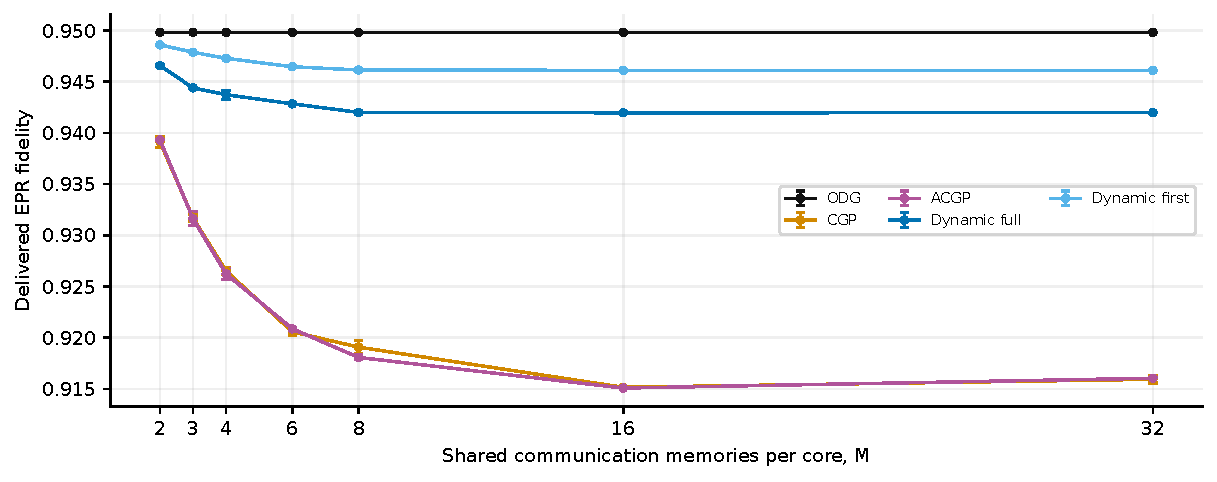
\includegraphics[width=.94\linewidth,height=.255\textheight,keepaspectratio]{figures/memory/mesh_yx_average_delivered_epr_fidelity.pdf}\captionof{figure}{Run-level mean and sample SD. Shared trace aliases are counted once.}\end{center}
\begin{center}{\scriptsize\setlength{\tabcolsep}{3pt}
\begin{tabular}{lrrrrr}
\toprule
M & ODG & CGP & ACGP & Dynamic full & Dynamic first \\
\midrule
2 & $0.9498\pm0.0000$ & $0.9391\pm0.0005$ & $0.9393\pm0.0000$ & $0.9466\pm0.0001$ & $0.9486\pm0.0000$ \\
3 & $0.9498\pm0.0000$ & $0.9317\pm0.0003$ & $0.9316\pm0.0007$ & $0.9444\pm0.0001$ & $0.9479\pm0.0000$ \\
4 & $0.9498\pm0.0000$ & $0.9265\pm0.0003$ & $0.9262\pm0.0006$ & $0.9437\pm0.0004$ & $0.9473\pm0.0000$ \\
6 & $0.9498\pm0.0000$ & $0.9206\pm0.0003$ & $0.9209\pm0.0001$ & $0.9428\pm0.0000$ & $0.9465\pm0.0001$ \\
8 & $0.9498\pm0.0000$ & $0.9191\pm0.0006$ & $0.9181\pm0.0002$ & $0.9420\pm0.0002$ & $0.9461\pm0.0000$ \\
16 & $0.9498\pm0.0000$ & $0.9152\pm0.0000$ & $0.9151\pm0.0001$ & $0.9420\pm0.0000$ & $0.9461\pm0.0000$ \\
32 & $0.9498\pm0.0000$ & $0.9159\pm0.0004$ & $0.9160\pm0.0000$ & $0.9420\pm0.0000$ & $0.9461\pm0.0000$ \\
\bottomrule\end{tabular}}
\captionof{table}{Mean $\pm$ sample SD; n/a denotes a metric outside that policy's instrumentation.}
{\footnotesize\href{https://github.com/sanjeevkrishnaa/Compiler-Driven-ACE/blob/codex/ace-scheduler-correctness/docs/latex/qft96_final/data/memory_mesh_yx_average_delivered_epr_fidelity.csv}{Exact CSV values and sample counts}}
\end{center}
\subsection*{Compiler readiness fraction}
\begin{center}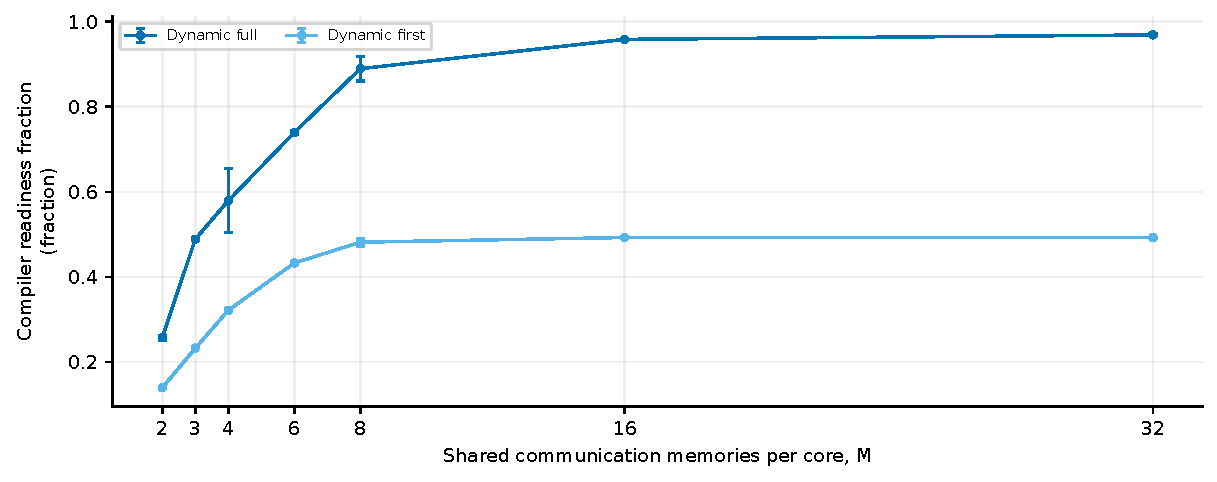
\includegraphics[width=.94\linewidth,height=.255\textheight,keepaspectratio]{figures/memory/mesh_yx_pregenerated_success_rate.pdf}\captionof{figure}{Run-level mean and sample SD. Shared trace aliases are counted once.}\end{center}
\begin{center}{\scriptsize\setlength{\tabcolsep}{3pt}
\begin{tabular}{lrrrrr}
\toprule
M & ODG & CGP & ACGP & Dynamic full & Dynamic first \\
\midrule
2 & n/a & n/a & n/a & $0.2571\pm0.0060$ & $0.1398\pm0.0026$ \\
3 & n/a & n/a & n/a & $0.4889\pm0.0004$ & $0.2328\pm0.0005$ \\
4 & n/a & n/a & n/a & $0.5795\pm0.0752$ & $0.3219\pm0.0020$ \\
6 & n/a & n/a & n/a & $0.7397\pm0.0044$ & $0.4329\pm0.0044$ \\
8 & n/a & n/a & n/a & $0.8894\pm0.0290$ & $0.4818\pm0.0097$ \\
16 & n/a & n/a & n/a & $0.9583\pm0.0027$ & $0.4928\pm0.0011$ \\
32 & n/a & n/a & n/a & $0.9688\pm0.0022$ & $0.4928\pm0.0011$ \\
\bottomrule\end{tabular}}
\captionof{table}{Mean $\pm$ sample SD; n/a denotes a metric outside that policy's instrumentation.}
{\footnotesize\href{https://github.com/sanjeevkrishnaa/Compiler-Driven-ACE/blob/codex/ace-scheduler-correctness/docs/latex/qft96_final/data/memory_mesh_yx_pregenerated_success_rate.csv}{Exact CSV values and sample counts}}
\end{center}
\clearpage
\subsection*{Intended compiler-hit fraction}
\begin{center}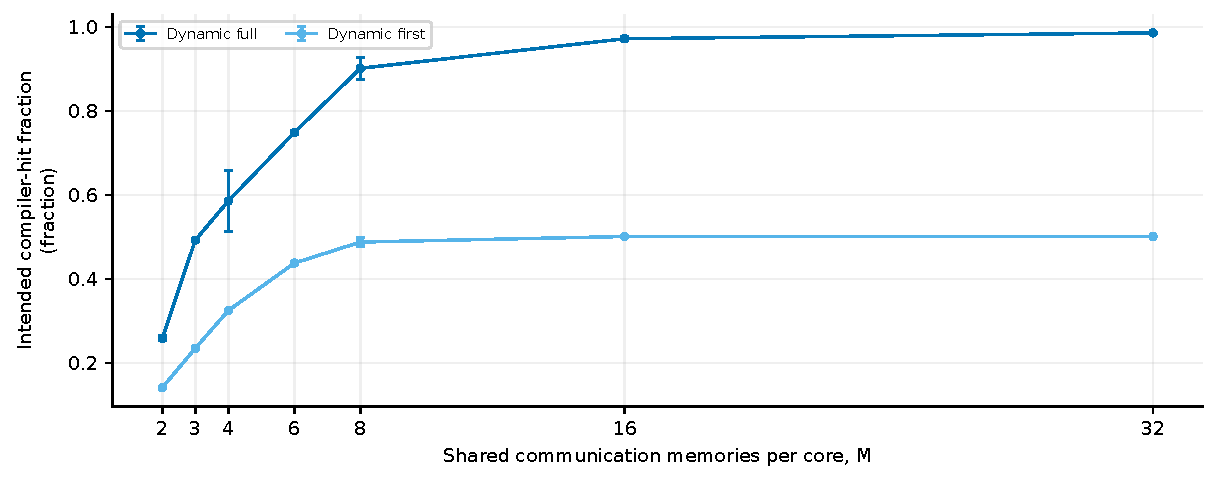
\includegraphics[width=.94\linewidth,height=.255\textheight,keepaspectratio]{figures/memory/mesh_yx_intended_request_hit_rate.pdf}\captionof{figure}{Run-level mean and sample SD. Shared trace aliases are counted once.}\end{center}
\begin{center}{\scriptsize\setlength{\tabcolsep}{3pt}
\begin{tabular}{lrrrrr}
\toprule
M & ODG & CGP & ACGP & Dynamic full & Dynamic first \\
\midrule
2 & n/a & n/a & n/a & $0.2585\pm0.0062$ & $0.1409\pm0.0026$ \\
3 & n/a & n/a & n/a & $0.4923\pm0.0015$ & $0.2346\pm0.0013$ \\
4 & n/a & n/a & n/a & $0.5857\pm0.0733$ & $0.3246\pm0.0007$ \\
6 & n/a & n/a & n/a & $0.7488\pm0.0042$ & $0.4377\pm0.0042$ \\
8 & n/a & n/a & n/a & $0.9017\pm0.0255$ & $0.4877\pm0.0104$ \\
16 & n/a & n/a & n/a & $0.9721\pm0.0044$ & $0.5010\pm0.0011$ \\
32 & n/a & n/a & n/a & $0.9862\pm0.0013$ & $0.5010\pm0.0011$ \\
\bottomrule\end{tabular}}
\captionof{table}{Mean $\pm$ sample SD; n/a denotes a metric outside that policy's instrumentation.}
{\footnotesize\href{https://github.com/sanjeevkrishnaa/Compiler-Driven-ACE/blob/codex/ace-scheduler-correctness/docs/latex/qft96_final/data/memory_mesh_yx_intended_request_hit_rate.csv}{Exact CSV values and sample counts}}
\end{center}
\subsection*{Compiler fallback fraction}
\begin{center}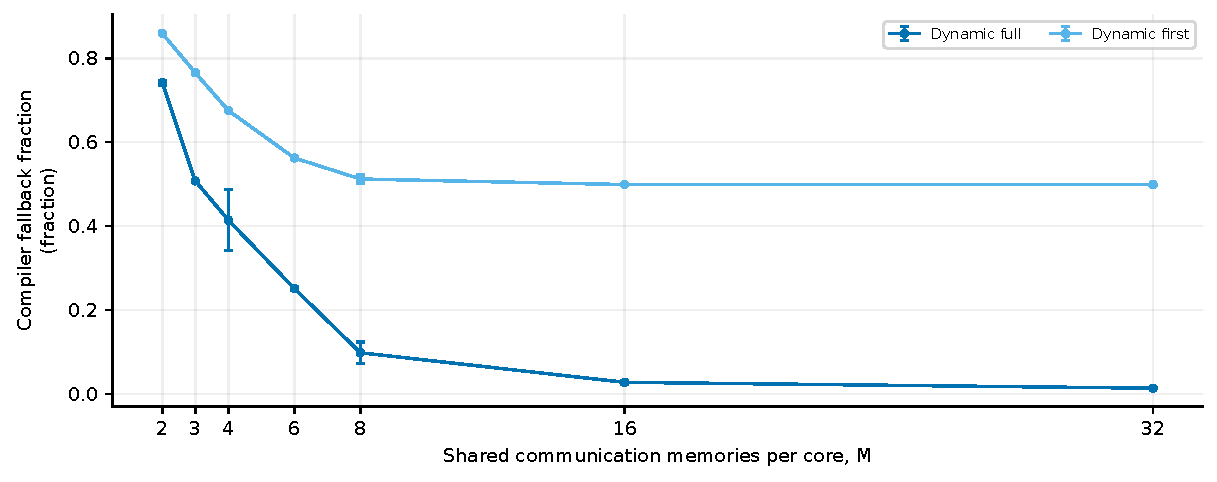
\includegraphics[width=.94\linewidth,height=.255\textheight,keepaspectratio]{figures/memory/mesh_yx_on_demand_fallback_rate.pdf}\captionof{figure}{Run-level mean and sample SD. Shared trace aliases are counted once.}\end{center}
\begin{center}{\scriptsize\setlength{\tabcolsep}{3pt}
\begin{tabular}{lrrrrr}
\toprule
M & ODG & CGP & ACGP & Dynamic full & Dynamic first \\
\midrule
2 & n/a & n/a & n/a & $0.7415\pm0.0062$ & $0.8591\pm0.0026$ \\
3 & n/a & n/a & n/a & $0.5077\pm0.0015$ & $0.7654\pm0.0013$ \\
4 & n/a & n/a & n/a & $0.4143\pm0.0733$ & $0.6754\pm0.0007$ \\
6 & n/a & n/a & n/a & $0.2512\pm0.0042$ & $0.5623\pm0.0042$ \\
8 & n/a & n/a & n/a & $0.0983\pm0.0255$ & $0.5123\pm0.0104$ \\
16 & n/a & n/a & n/a & $0.0279\pm0.0044$ & $0.4990\pm0.0011$ \\
32 & n/a & n/a & n/a & $0.0138\pm0.0013$ & $0.4990\pm0.0011$ \\
\bottomrule\end{tabular}}
\captionof{table}{Mean $\pm$ sample SD; n/a denotes a metric outside that policy's instrumentation.}
{\footnotesize\href{https://github.com/sanjeevkrishnaa/Compiler-Driven-ACE/blob/codex/ace-scheduler-correctness/docs/latex/qft96_final/data/memory_mesh_yx_on_demand_fallback_rate.csv}{Exact CSV values and sample counts}}
\end{center}
\clearpage
\subsection*{Compiler-cache waste}
\begin{center}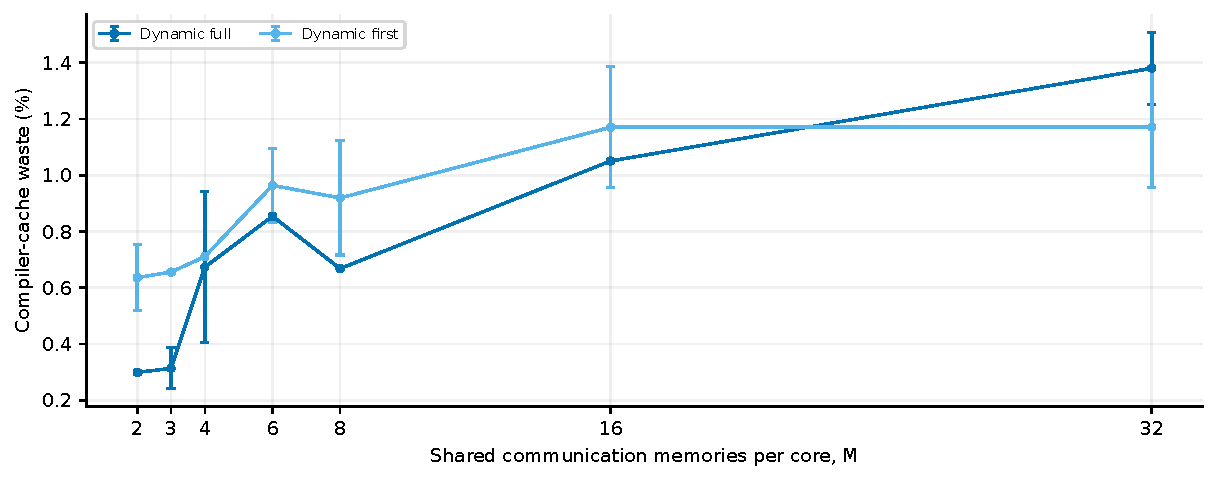
\includegraphics[width=.94\linewidth,height=.255\textheight,keepaspectratio]{figures/memory/mesh_yx_compiler_waste_percentage.pdf}\captionof{figure}{Run-level mean and sample SD. Shared trace aliases are counted once.}\end{center}
\begin{center}{\scriptsize\setlength{\tabcolsep}{3pt}
\begin{tabular}{lrrrrr}
\toprule
M & ODG & CGP & ACGP & Dynamic full & Dynamic first \\
\midrule
2 & n/a & n/a & n/a & $0.2986\pm0.0071$ & $0.6358\pm0.1164$ \\
3 & n/a & n/a & n/a & $0.3133\pm0.0727$ & $0.6554\pm0.0035$ \\
4 & n/a & n/a & n/a & $0.6729\pm0.2681$ & $0.7103\pm0.0016$ \\
6 & n/a & n/a & n/a & $0.8540\pm0.0047$ & $0.9638\pm0.1318$ \\
8 & n/a & n/a & n/a & $0.6679\pm0.0012$ & $0.9191\pm0.2030$ \\
16 & n/a & n/a & n/a & $1.050\pm0.005$ & $1.170\pm0.216$ \\
32 & n/a & n/a & n/a & $1.380\pm0.128$ & $1.170\pm0.216$ \\
\bottomrule\end{tabular}}
\captionof{table}{Mean $\pm$ sample SD; n/a denotes a metric outside that policy's instrumentation.}
{\footnotesize\href{https://github.com/sanjeevkrishnaa/Compiler-Driven-ACE/blob/codex/ace-scheduler-correctness/docs/latex/qft96_final/data/memory_mesh_yx_compiler_waste_percentage.csv}{Exact CSV values and sample counts}}
\end{center}
\subsection*{Native-protocol waste}
\begin{center}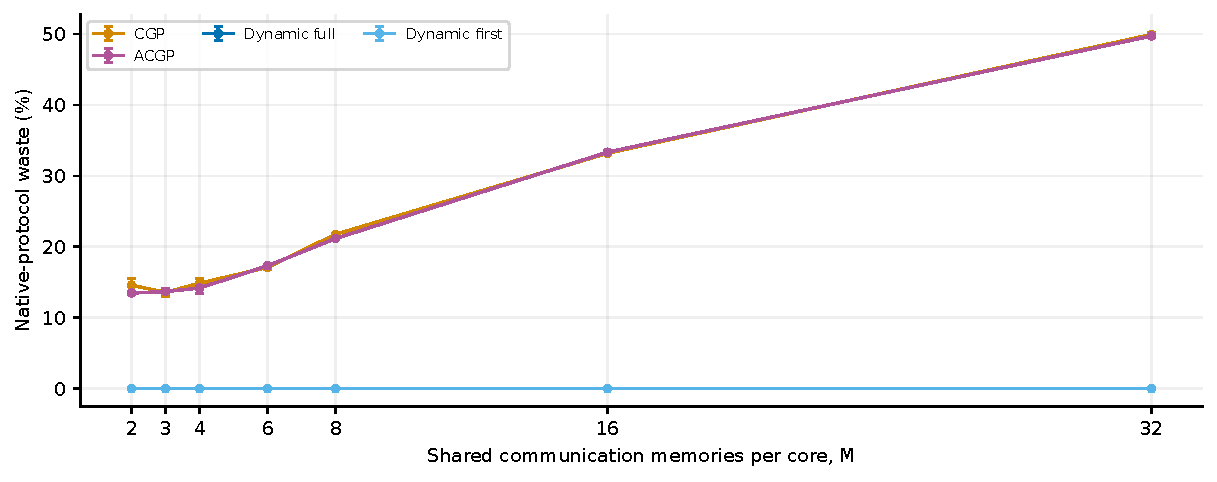
\includegraphics[width=.94\linewidth,height=.255\textheight,keepaspectratio]{figures/memory/mesh_yx_protocol_waste_percentage.pdf}\captionof{figure}{Run-level mean and sample SD. Shared trace aliases are counted once.}\end{center}
\begin{center}{\scriptsize\setlength{\tabcolsep}{3pt}
\begin{tabular}{lrrrrr}
\toprule
M & ODG & CGP & ACGP & Dynamic full & Dynamic first \\
\midrule
2 & n/a & $14.584\pm0.965$ & $13.483\pm0.264$ & $0.0000\pm0.0000$ & $0.0000\pm0.0000$ \\
3 & n/a & $13.576\pm0.514$ & $13.689\pm0.374$ & $0.0000\pm0.0000$ & $0.0000\pm0.0000$ \\
4 & n/a & $14.863\pm0.627$ & $14.186\pm0.779$ & $0.0000\pm0.0000$ & $0.0000\pm0.0000$ \\
6 & n/a & $17.093\pm0.215$ & $17.325\pm0.096$ & $0.0000\pm0.0000$ & $0.0000\pm0.0000$ \\
8 & n/a & $21.758\pm0.013$ & $21.168\pm0.053$ & $0.0000\pm0.0000$ & $0.0000\pm0.0000$ \\
16 & n/a & $33.183\pm0.156$ & $33.336\pm0.069$ & $0.0000\pm0.0000$ & $0.0000\pm0.0000$ \\
32 & n/a & $49.910\pm0.312$ & $49.715\pm0.211$ & $0.0000\pm0.0000$ & $0.0000\pm0.0000$ \\
\bottomrule\end{tabular}}
\captionof{table}{Mean $\pm$ sample SD; n/a denotes a metric outside that policy's instrumentation.}
{\footnotesize\href{https://github.com/sanjeevkrishnaa/Compiler-Driven-ACE/blob/codex/ace-scheduler-correctness/docs/latex/qft96_final/data/memory_mesh_yx_protocol_waste_percentage.csv}{Exact CSV values and sample counts}}
\end{center}
\clearpage
\subsection*{Compiler-pair expiry}
\begin{center}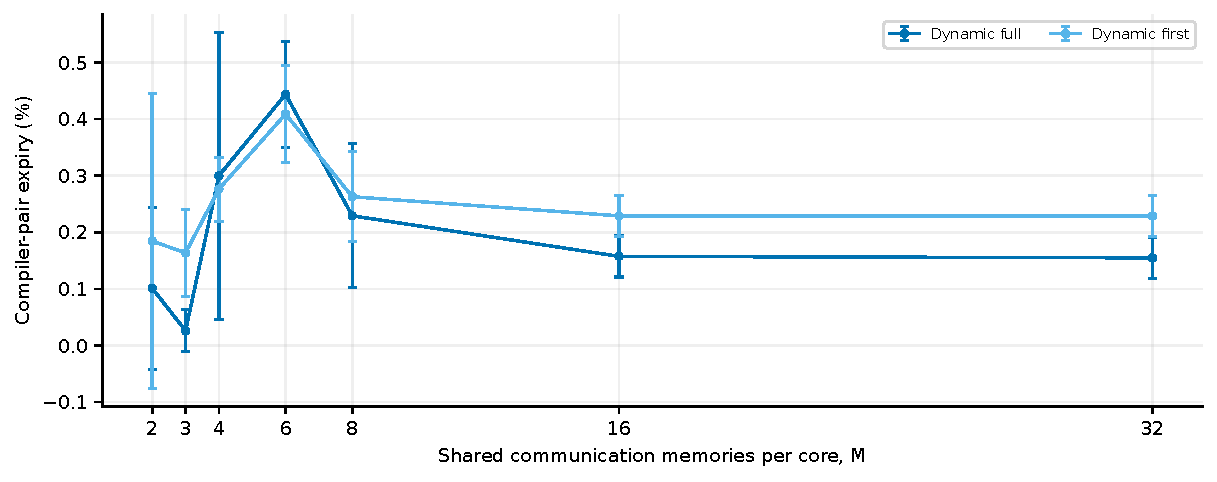
\includegraphics[width=.94\linewidth,height=.255\textheight,keepaspectratio]{figures/memory/mesh_yx_compiler_expiry_percentage.pdf}\captionof{figure}{Run-level mean and sample SD. Shared trace aliases are counted once.}\end{center}
\begin{center}{\scriptsize\setlength{\tabcolsep}{3pt}
\begin{tabular}{lrrrrr}
\toprule
M & ODG & CGP & ACGP & Dynamic full & Dynamic first \\
\midrule
2 & n/a & n/a & n/a & $0.1012\pm0.1431$ & $0.1845\pm0.2609$ \\
3 & n/a & n/a & n/a & $0.0261\pm0.0368$ & $0.1636\pm0.0764$ \\
4 & n/a & n/a & n/a & $0.3000\pm0.2534$ & $0.2763\pm0.0564$ \\
6 & n/a & n/a & n/a & $0.4438\pm0.0942$ & $0.4090\pm0.0859$ \\
8 & n/a & n/a & n/a & $0.2292\pm0.1271$ & $0.2628\pm0.0792$ \\
16 & n/a & n/a & n/a & $0.1575\pm0.0364$ & $0.2290\pm0.0360$ \\
32 & n/a & n/a & n/a & $0.1548\pm0.0365$ & $0.2290\pm0.0360$ \\
\bottomrule\end{tabular}}
\captionof{table}{Mean $\pm$ sample SD; n/a denotes a metric outside that policy's instrumentation.}
{\footnotesize\href{https://github.com/sanjeevkrishnaa/Compiler-Driven-ACE/blob/codex/ace-scheduler-correctness/docs/latex/qft96_final/data/memory_mesh_yx_compiler_expiry_percentage.csv}{Exact CSV values and sample counts}}
\end{center}
\subsection*{Used compiler-pair storage time}
\begin{center}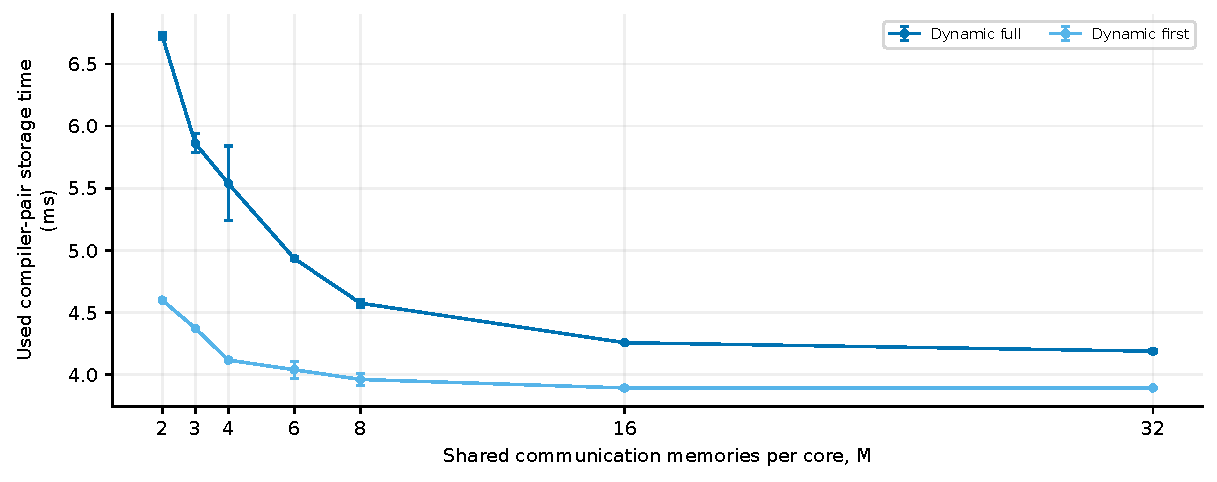
\includegraphics[width=.94\linewidth,height=.255\textheight,keepaspectratio]{figures/memory/mesh_yx_average_storage_time_ms.pdf}\captionof{figure}{Run-level mean and sample SD. Shared trace aliases are counted once.}\end{center}
\begin{center}{\scriptsize\setlength{\tabcolsep}{3pt}
\begin{tabular}{lrrrrr}
\toprule
M & ODG & CGP & ACGP & Dynamic full & Dynamic first \\
\midrule
2 & n/a & n/a & n/a & $6.726\pm0.029$ & $4.600\pm0.012$ \\
3 & n/a & n/a & n/a & $5.862\pm0.078$ & $4.374\pm0.004$ \\
4 & n/a & n/a & n/a & $5.539\pm0.301$ & $4.118\pm0.008$ \\
6 & n/a & n/a & n/a & $4.935\pm0.013$ & $4.040\pm0.067$ \\
8 & n/a & n/a & n/a & $4.576\pm0.031$ & $3.962\pm0.045$ \\
16 & n/a & n/a & n/a & $4.258\pm0.004$ & $3.894\pm0.006$ \\
32 & n/a & n/a & n/a & $4.189\pm0.010$ & $3.894\pm0.006$ \\
\bottomrule\end{tabular}}
\captionof{table}{Mean $\pm$ sample SD; n/a denotes a metric outside that policy's instrumentation.}
{\footnotesize\href{https://github.com/sanjeevkrishnaa/Compiler-Driven-ACE/blob/codex/ace-scheduler-correctness/docs/latex/qft96_final/data/memory_mesh_yx_average_storage_time_ms.csv}{Exact CSV values and sample counts}}
\end{center}
\clearpage
\subsection*{Delivered-hop throughput}
\begin{center}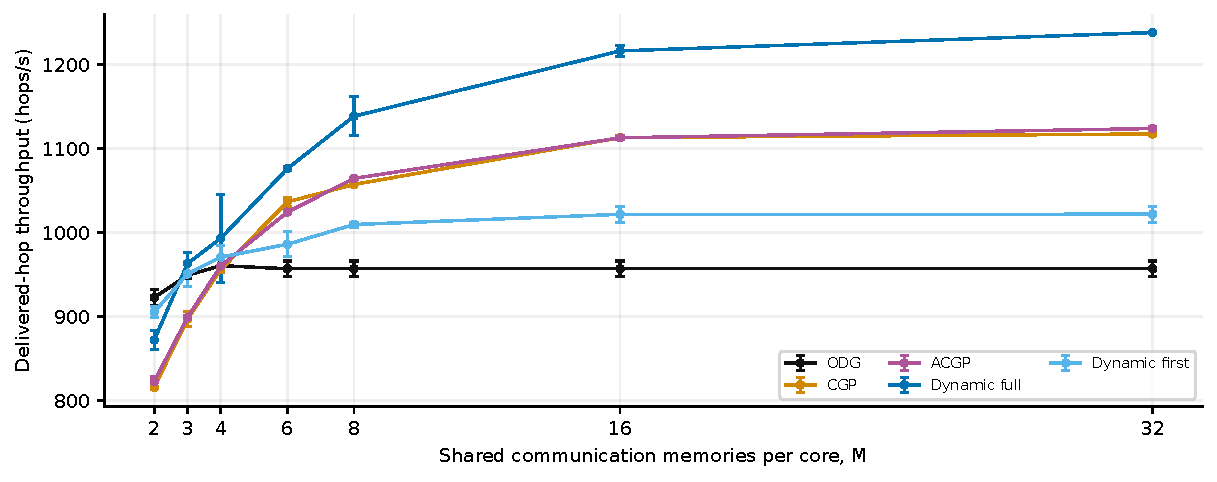
\includegraphics[width=.94\linewidth,height=.255\textheight,keepaspectratio]{figures/memory/mesh_yx_hop_throughput_s.pdf}\captionof{figure}{Run-level mean and sample SD. Shared trace aliases are counted once.}\end{center}
\begin{center}{\scriptsize\setlength{\tabcolsep}{3pt}
\begin{tabular}{lrrrrr}
\toprule
M & ODG & CGP & ACGP & Dynamic full & Dynamic first \\
\midrule
2 & $922.64\pm9.60$ & $815.59\pm1.56$ & $822.74\pm6.27$ & $872.09\pm11.45$ & $905.17\pm6.74$ \\
3 & $949.24\pm4.06$ & $897.11\pm9.06$ & $898.90\pm2.79$ & $962.99\pm13.06$ & $950.73\pm15.02$ \\
4 & $960.49\pm7.66$ & $955.82\pm1.48$ & $960.24\pm7.66$ & $993.15\pm52.58$ & $970.68\pm14.08$ \\
6 & $956.85\pm9.24$ & $1036.39\pm5.06$ & $1024.22\pm1.73$ & $1075.89\pm2.53$ & $985.97\pm15.04$ \\
8 & $956.85\pm9.24$ & $1057.15\pm0.59$ & $1064.32\pm1.21$ & $1138.33\pm23.35$ & $1009.43\pm2.90$ \\
16 & $956.85\pm9.24$ & $1112.88\pm0.48$ & $1112.65\pm2.46$ & $1216.05\pm6.42$ & $1021.60\pm9.41$ \\
32 & $956.85\pm9.24$ & $1117.24\pm2.01$ & $1123.71\pm2.26$ & $1237.92\pm0.25$ & $1021.71\pm9.56$ \\
\bottomrule\end{tabular}}
\captionof{table}{Mean $\pm$ sample SD; n/a denotes a metric outside that policy's instrumentation.}
{\footnotesize\href{https://github.com/sanjeevkrishnaa/Compiler-Driven-ACE/blob/codex/ace-scheduler-correctness/docs/latex/qft96_final/data/memory_mesh_yx_hop_throughput_s.csv}{Exact CSV values and sample counts}}
\end{center}
\subsection*{Completion fraction}
\begin{center}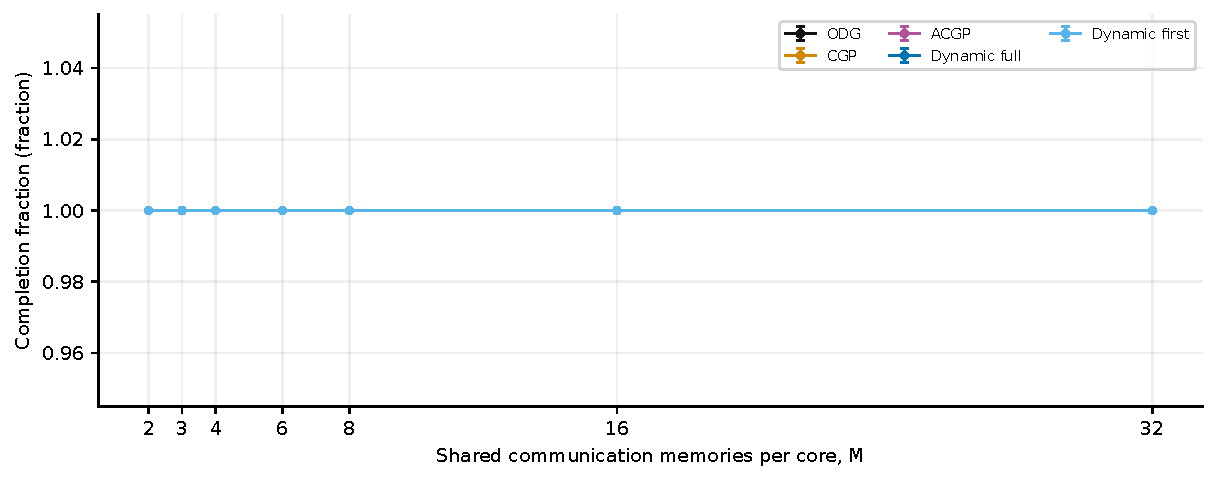
\includegraphics[width=.94\linewidth,height=.255\textheight,keepaspectratio]{figures/memory/mesh_yx_completion_rate.pdf}\captionof{figure}{Run-level mean and sample SD. Shared trace aliases are counted once.}\end{center}
\begin{center}{\scriptsize\setlength{\tabcolsep}{3pt}
\begin{tabular}{lrrrrr}
\toprule
M & ODG & CGP & ACGP & Dynamic full & Dynamic first \\
\midrule
2 & $1.000\pm0.000$ & $1.000\pm0.000$ & $1.000\pm0.000$ & $1.000\pm0.000$ & $1.000\pm0.000$ \\
3 & $1.000\pm0.000$ & $1.000\pm0.000$ & $1.000\pm0.000$ & $1.000\pm0.000$ & $1.000\pm0.000$ \\
4 & $1.000\pm0.000$ & $1.000\pm0.000$ & $1.000\pm0.000$ & $1.000\pm0.000$ & $1.000\pm0.000$ \\
6 & $1.000\pm0.000$ & $1.000\pm0.000$ & $1.000\pm0.000$ & $1.000\pm0.000$ & $1.000\pm0.000$ \\
8 & $1.000\pm0.000$ & $1.000\pm0.000$ & $1.000\pm0.000$ & $1.000\pm0.000$ & $1.000\pm0.000$ \\
16 & $1.000\pm0.000$ & $1.000\pm0.000$ & $1.000\pm0.000$ & $1.000\pm0.000$ & $1.000\pm0.000$ \\
32 & $1.000\pm0.000$ & $1.000\pm0.000$ & $1.000\pm0.000$ & $1.000\pm0.000$ & $1.000\pm0.000$ \\
\bottomrule\end{tabular}}
\captionof{table}{Mean $\pm$ sample SD; n/a denotes a metric outside that policy's instrumentation.}
{\footnotesize\href{https://github.com/sanjeevkrishnaa/Compiler-Driven-ACE/blob/codex/ace-scheduler-correctness/docs/latex/qft96_final/data/memory_mesh_yx_completion_rate.csv}{Exact CSV values and sample counts}}
\end{center}
\clearpage
\subsection*{Maximum admission wait}
\begin{center}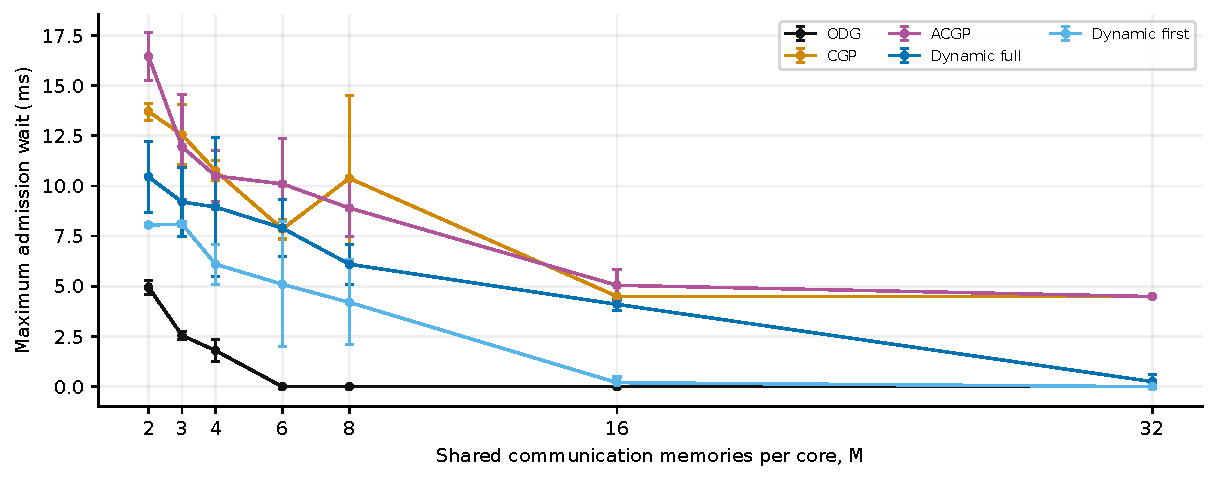
\includegraphics[width=.94\linewidth,height=.255\textheight,keepaspectratio]{figures/memory/mesh_yx_max_admission_wait_ms.pdf}\captionof{figure}{Run-level mean and sample SD. Shared trace aliases are counted once.}\end{center}
\begin{center}{\scriptsize\setlength{\tabcolsep}{3pt}
\begin{tabular}{lrrrrr}
\toprule
M & ODG & CGP & ACGP & Dynamic full & Dynamic first \\
\midrule
2 & $4.950\pm0.354$ & $13.700\pm0.424$ & $16.450\pm1.202$ & $10.450\pm1.768$ & $8.050\pm0.071$ \\
3 & $2.550\pm0.212$ & $12.550\pm1.485$ & $11.950\pm2.616$ & $9.200\pm1.697$ & $8.100\pm0.141$ \\
4 & $1.800\pm0.566$ & $10.752\pm0.497$ & $10.500\pm1.273$ & $8.950\pm3.465$ & $6.100\pm0.990$ \\
6 & $0.0000\pm0.0000$ & $7.850\pm0.495$ & $10.100\pm2.263$ & $7.900\pm1.414$ & $5.100\pm3.111$ \\
8 & $0.0000\pm0.0000$ & $10.382\pm4.127$ & $8.900\pm1.414$ & $6.100\pm0.990$ & $4.200\pm2.121$ \\
16 & $0.0000\pm0.0000$ & $4.500\pm0.000$ & $5.050\pm0.778$ & $4.100\pm0.283$ & $0.2000\pm0.2828$ \\
32 & $0.0000\pm0.0000$ & $4.500\pm0.000$ & $4.489\pm0.016$ & $0.2500\pm0.3536$ & $0.0000\pm0.0000$ \\
\bottomrule\end{tabular}}
\captionof{table}{Mean $\pm$ sample SD; n/a denotes a metric outside that policy's instrumentation.}
{\footnotesize\href{https://github.com/sanjeevkrishnaa/Compiler-Driven-ACE/blob/codex/ace-scheduler-correctness/docs/latex/qft96_final/data/memory_mesh_yx_max_admission_wait_ms.csv}{Exact CSV values and sample counts}}
\end{center}
\subsection*{Requests with admission wait}
\begin{center}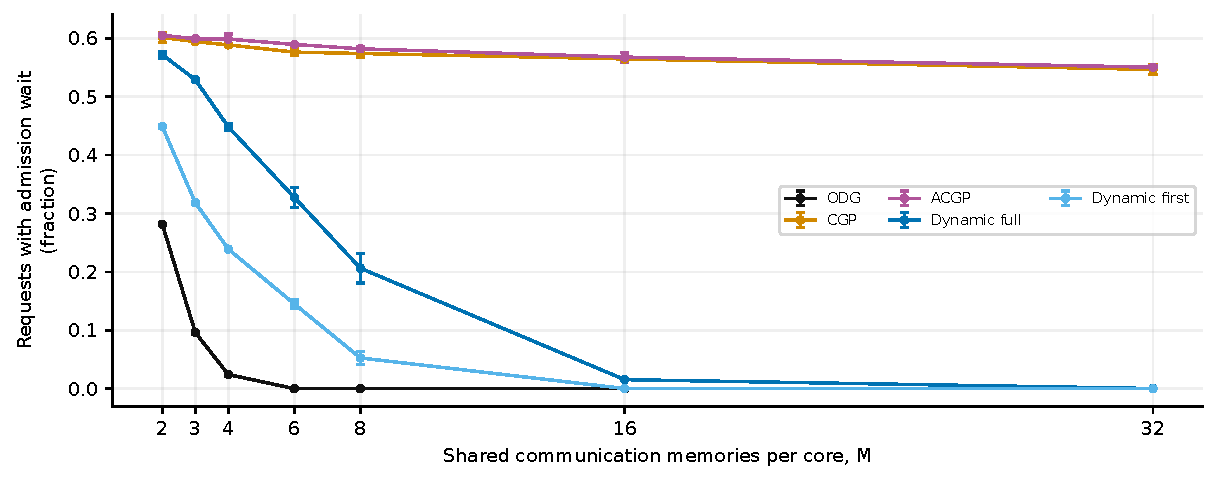
\includegraphics[width=.94\linewidth,height=.255\textheight,keepaspectratio]{figures/memory/mesh_yx_requests_that_waited_fraction.pdf}\captionof{figure}{Run-level mean and sample SD. Shared trace aliases are counted once.}\end{center}
\begin{center}{\scriptsize\setlength{\tabcolsep}{3pt}
\begin{tabular}{lrrrrr}
\toprule
M & ODG & CGP & ACGP & Dynamic full & Dynamic first \\
\midrule
2 & $0.2816\pm0.0009$ & $0.6014\pm0.0088$ & $0.6050\pm0.0018$ & $0.5719\pm0.0057$ & $0.4489\pm0.0018$ \\
3 & $0.0962\pm0.0022$ & $0.5942\pm0.0011$ & $0.5992\pm0.0027$ & $0.5290\pm0.0005$ & $0.3185\pm0.0024$ \\
4 & $0.0243\pm0.0000$ & $0.5886\pm0.0024$ & $0.5986\pm0.0088$ & $0.4483\pm0.0064$ & $0.2389\pm0.0007$ \\
6 & $0.0000\pm0.0000$ & $0.5762\pm0.0060$ & $0.5894\pm0.0024$ & $0.3274\pm0.0175$ & $0.1451\pm0.0071$ \\
8 & $0.0000\pm0.0000$ & $0.5739\pm0.0075$ & $0.5819\pm0.0038$ & $0.2063\pm0.0254$ & $0.0526\pm0.0117$ \\
16 & $0.0000\pm0.0000$ & $0.5646\pm0.0009$ & $0.5677\pm0.0086$ & $0.0155\pm0.0022$ & $0.0003\pm0.0004$ \\
32 & $0.0000\pm0.0000$ & $0.5466\pm0.0078$ & $0.5504\pm0.0020$ & $0.0003\pm0.0004$ & $0.0000\pm0.0000$ \\
\bottomrule\end{tabular}}
\captionof{table}{Mean $\pm$ sample SD; n/a denotes a metric outside that policy's instrumentation.}
{\footnotesize\href{https://github.com/sanjeevkrishnaa/Compiler-Driven-ACE/blob/codex/ace-scheduler-correctness/docs/latex/qft96_final/data/memory_mesh_yx_requests_that_waited_fraction.csv}{Exact CSV values and sample counts}}
\end{center}
\clearpage
\subsection*{Recorded reservation-setup counter}
\begin{center}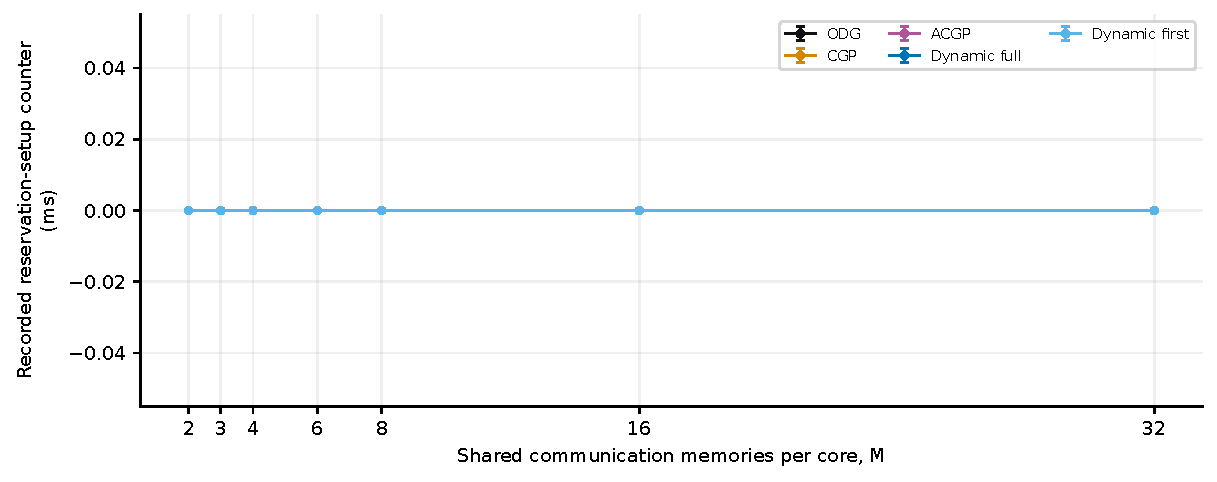
\includegraphics[width=.94\linewidth,height=.255\textheight,keepaspectratio]{figures/memory/mesh_yx_avg_reservation_setup_time_ms.pdf}\captionof{figure}{Run-level mean and sample SD. Shared trace aliases are counted once.}\end{center}
\begin{center}{\scriptsize\setlength{\tabcolsep}{3pt}
\begin{tabular}{lrrrrr}
\toprule
M & ODG & CGP & ACGP & Dynamic full & Dynamic first \\
\midrule
2 & $0.0000\pm0.0000$ & $0.0000\pm0.0000$ & $0.0000\pm0.0000$ & $0.0000\pm0.0000$ & $0.0000\pm0.0000$ \\
3 & $0.0000\pm0.0000$ & $0.0000\pm0.0000$ & $0.0000\pm0.0000$ & $0.0000\pm0.0000$ & $0.0000\pm0.0000$ \\
4 & $0.0000\pm0.0000$ & $0.0000\pm0.0000$ & $0.0000\pm0.0000$ & $0.0000\pm0.0000$ & $0.0000\pm0.0000$ \\
6 & $0.0000\pm0.0000$ & $0.0000\pm0.0000$ & $0.0000\pm0.0000$ & $0.0000\pm0.0000$ & $0.0000\pm0.0000$ \\
8 & $0.0000\pm0.0000$ & $0.0000\pm0.0000$ & $0.0000\pm0.0000$ & $0.0000\pm0.0000$ & $0.0000\pm0.0000$ \\
16 & $0.0000\pm0.0000$ & $0.0000\pm0.0000$ & $0.0000\pm0.0000$ & $0.0000\pm0.0000$ & $0.0000\pm0.0000$ \\
32 & $0.0000\pm0.0000$ & $0.0000\pm0.0000$ & $0.0000\pm0.0000$ & $0.0000\pm0.0000$ & $0.0000\pm0.0000$ \\
\bottomrule\end{tabular}}
\captionof{table}{Mean $\pm$ sample SD; n/a denotes a metric outside that policy's instrumentation.}
{\footnotesize\href{https://github.com/sanjeevkrishnaa/Compiler-Driven-ACE/blob/codex/ace-scheduler-correctness/docs/latex/qft96_final/data/memory_mesh_yx_avg_reservation_setup_time_ms.csv}{Exact CSV values and sample counts}}
\end{center}
\subsection*{Mean generation/service time}
\begin{center}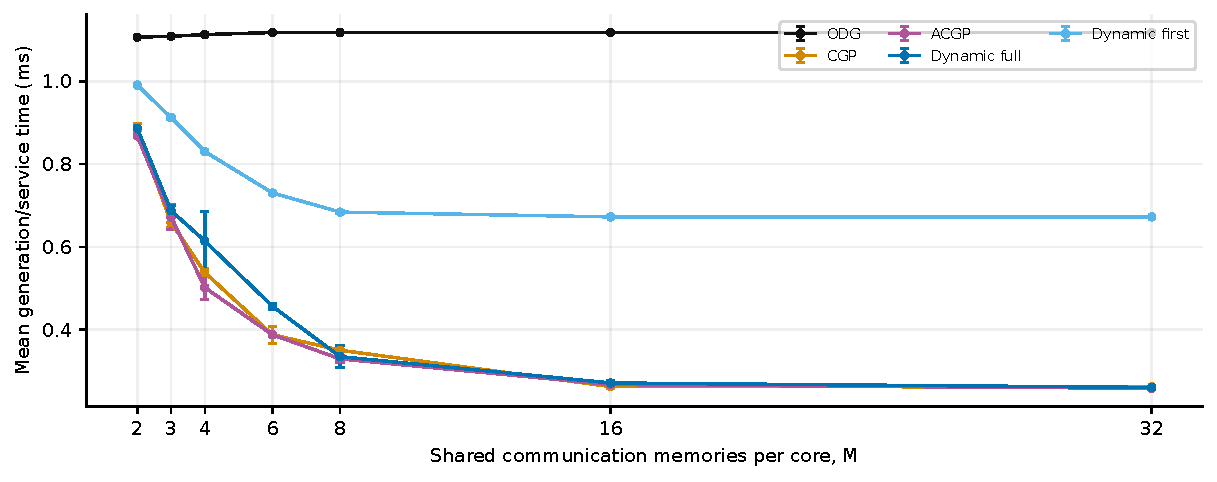
\includegraphics[width=.94\linewidth,height=.255\textheight,keepaspectratio]{figures/memory/mesh_yx_avg_entanglement_generation_time_ms.pdf}\captionof{figure}{Run-level mean and sample SD. Shared trace aliases are counted once.}\end{center}
\begin{center}{\scriptsize\setlength{\tabcolsep}{3pt}
\begin{tabular}{lrrrrr}
\toprule
M & ODG & CGP & ACGP & Dynamic full & Dynamic first \\
\midrule
2 & $1.106\pm0.000$ & $0.8831\pm0.0155$ & $0.8679\pm0.0006$ & $0.8866\pm0.0024$ & $0.9907\pm0.0007$ \\
3 & $1.109\pm0.000$ & $0.6591\pm0.0124$ & $0.6720\pm0.0296$ & $0.6876\pm0.0120$ & $0.9122\pm0.0037$ \\
4 & $1.113\pm0.002$ & $0.5381\pm0.0104$ & $0.5018\pm0.0279$ & $0.6142\pm0.0718$ & $0.8301\pm0.0028$ \\
6 & $1.118\pm0.000$ & $0.3878\pm0.0210$ & $0.3878\pm0.0002$ & $0.4565\pm0.0067$ & $0.7303\pm0.0022$ \\
8 & $1.118\pm0.000$ & $0.3505\pm0.0028$ & $0.3295\pm0.0074$ & $0.3349\pm0.0267$ & $0.6840\pm0.0037$ \\
16 & $1.118\pm0.000$ & $0.2627\pm0.0052$ & $0.2676\pm0.0012$ & $0.2715\pm0.0052$ & $0.6724\pm0.0011$ \\
32 & $1.118\pm0.000$ & $0.2620\pm0.0002$ & $0.2585\pm0.0008$ & $0.2606\pm0.0010$ & $0.6724\pm0.0011$ \\
\bottomrule\end{tabular}}
\captionof{table}{Mean $\pm$ sample SD; n/a denotes a metric outside that policy's instrumentation.}
{\footnotesize\href{https://github.com/sanjeevkrishnaa/Compiler-Driven-ACE/blob/codex/ace-scheduler-correctness/docs/latex/qft96_final/data/memory_mesh_yx_avg_entanglement_generation_time_ms.csv}{Exact CSV values and sample counts}}
\end{center}
\clearpage
\subsection*{Recorded retry-wait time}
\begin{center}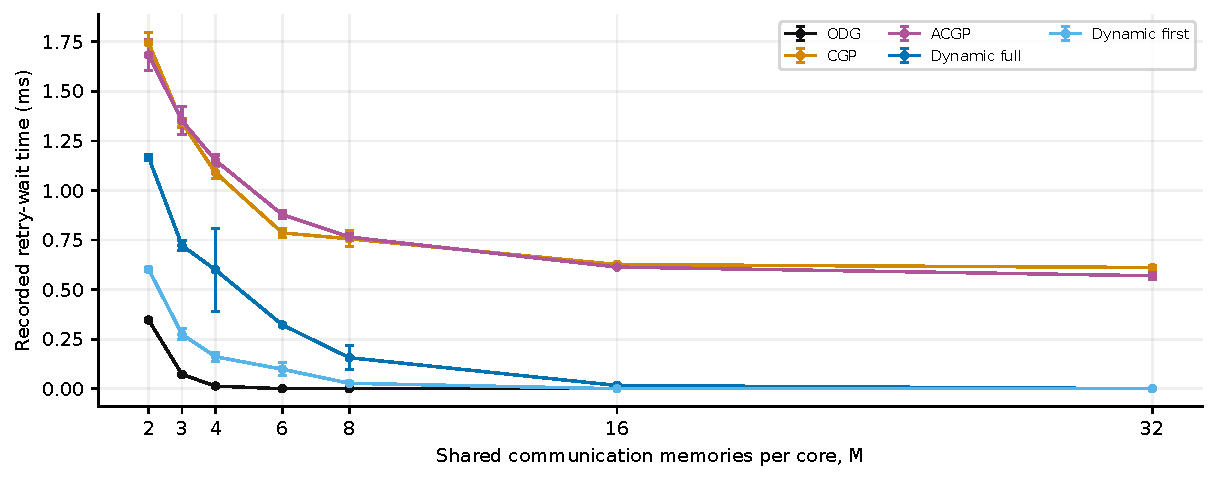
\includegraphics[width=.94\linewidth,height=.255\textheight,keepaspectratio]{figures/memory/mesh_yx_avg_retry_wait_time_ms.pdf}\captionof{figure}{Run-level mean and sample SD. Shared trace aliases are counted once.}\end{center}
\begin{center}{\scriptsize\setlength{\tabcolsep}{3pt}
\begin{tabular}{lrrrrr}
\toprule
M & ODG & CGP & ACGP & Dynamic full & Dynamic first \\
\midrule
2 & $0.3471\pm0.0048$ & $1.744\pm0.054$ & $1.683\pm0.077$ & $1.167\pm0.016$ & $0.6028\pm0.0088$ \\
3 & $0.0722\pm0.0055$ & $1.343\pm0.022$ & $1.352\pm0.069$ & $0.7225\pm0.0260$ & $0.2750\pm0.0290$ \\
4 & $0.0133\pm0.0009$ & $1.090\pm0.030$ & $1.152\pm0.027$ & $0.5996\pm0.2099$ & $0.1616\pm0.0227$ \\
6 & $0.0000\pm0.0000$ & $0.7861\pm0.0227$ & $0.8781\pm0.0188$ & $0.3220\pm0.0051$ & $0.0983\pm0.0326$ \\
8 & $0.0000\pm0.0000$ & $0.7562\pm0.0396$ & $0.7651\pm0.0183$ & $0.1567\pm0.0618$ & $0.0275\pm0.0080$ \\
16 & $0.0000\pm0.0000$ & $0.6264\pm0.0058$ & $0.6138\pm0.0041$ & $0.0165\pm0.0049$ & $0.0001\pm0.0001$ \\
32 & $0.0000\pm0.0000$ & $0.6115\pm0.0121$ & $0.5697\pm0.0179$ & $0.0001\pm0.0002$ & $0.0000\pm0.0000$ \\
\bottomrule\end{tabular}}
\captionof{table}{Mean $\pm$ sample SD; n/a denotes a metric outside that policy's instrumentation.}
{\footnotesize\href{https://github.com/sanjeevkrishnaa/Compiler-Driven-ACE/blob/codex/ace-scheduler-correctness/docs/latex/qft96_final/data/memory_mesh_yx_avg_retry_wait_time_ms.csv}{Exact CSV values and sample counts}}
\end{center}
\subsection*{Request retries}
\begin{center}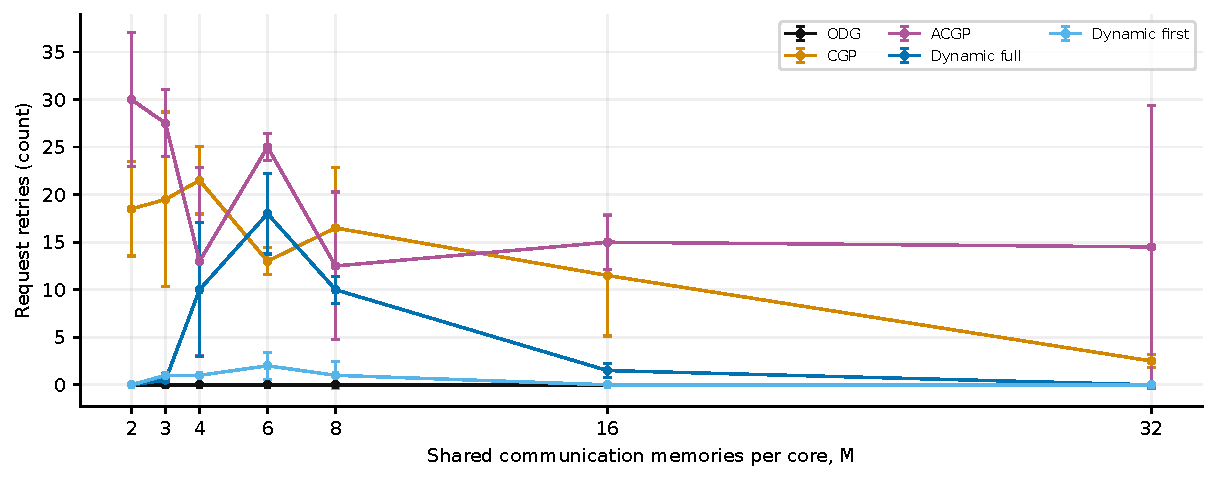
\includegraphics[width=.94\linewidth,height=.255\textheight,keepaspectratio]{figures/memory/mesh_yx_total_retries.pdf}\captionof{figure}{Run-level mean and sample SD. Shared trace aliases are counted once.}\end{center}
\begin{center}{\scriptsize\setlength{\tabcolsep}{3pt}
\begin{tabular}{lrrrrr}
\toprule
M & ODG & CGP & ACGP & Dynamic full & Dynamic first \\
\midrule
2 & $0.0000\pm0.0000$ & $18.500\pm4.950$ & $30.000\pm7.071$ & $0.0000\pm0.0000$ & $0.0000\pm0.0000$ \\
3 & $0.0000\pm0.0000$ & $19.500\pm9.192$ & $27.500\pm3.536$ & $0.5000\pm0.7071$ & $1.000\pm0.000$ \\
4 & $0.0000\pm0.0000$ & $21.500\pm3.536$ & $13.000\pm9.899$ & $10.000\pm7.071$ & $1.000\pm0.000$ \\
6 & $0.0000\pm0.0000$ & $13.000\pm1.414$ & $25.000\pm1.414$ & $18.000\pm4.243$ & $2.000\pm1.414$ \\
8 & $0.0000\pm0.0000$ & $16.500\pm6.364$ & $12.500\pm7.778$ & $10.000\pm1.414$ & $1.000\pm1.414$ \\
16 & $0.0000\pm0.0000$ & $11.500\pm6.364$ & $15.000\pm2.828$ & $1.500\pm0.707$ & $0.0000\pm0.0000$ \\
32 & $0.0000\pm0.0000$ & $2.500\pm0.707$ & $14.500\pm14.849$ & $0.0000\pm0.0000$ & $0.0000\pm0.0000$ \\
\bottomrule\end{tabular}}
\captionof{table}{Mean $\pm$ sample SD; n/a denotes a metric outside that policy's instrumentation.}
{\footnotesize\href{https://github.com/sanjeevkrishnaa/Compiler-Driven-ACE/blob/codex/ace-scheduler-correctness/docs/latex/qft96_final/data/memory_mesh_yx_total_retries.csv}{Exact CSV values and sample counts}}
\end{center}
\clearpage
\subsection*{Requests with retries}
\begin{center}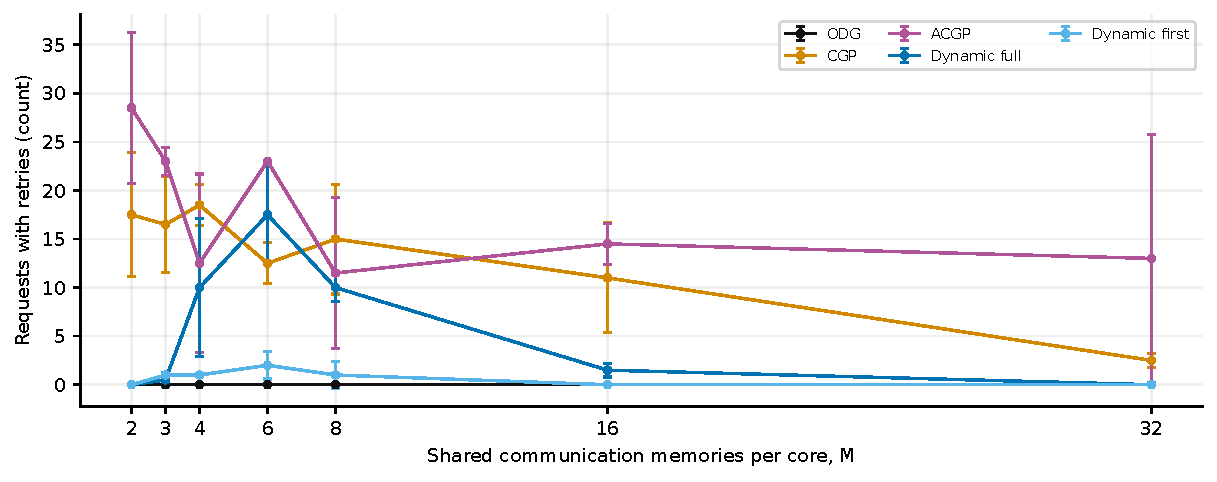
\includegraphics[width=.94\linewidth,height=.255\textheight,keepaspectratio]{figures/memory/mesh_yx_requests_with_retries.pdf}\captionof{figure}{Run-level mean and sample SD. Shared trace aliases are counted once.}\end{center}
\begin{center}{\scriptsize\setlength{\tabcolsep}{3pt}
\begin{tabular}{lrrrrr}
\toprule
M & ODG & CGP & ACGP & Dynamic full & Dynamic first \\
\midrule
2 & $0.0000\pm0.0000$ & $17.500\pm6.364$ & $28.500\pm7.778$ & $0.0000\pm0.0000$ & $0.0000\pm0.0000$ \\
3 & $0.0000\pm0.0000$ & $16.500\pm4.950$ & $23.000\pm1.414$ & $0.5000\pm0.7071$ & $1.000\pm0.000$ \\
4 & $0.0000\pm0.0000$ & $18.500\pm2.121$ & $12.500\pm9.192$ & $10.000\pm7.071$ & $1.000\pm0.000$ \\
6 & $0.0000\pm0.0000$ & $12.500\pm2.121$ & $23.000\pm0.000$ & $17.500\pm4.950$ & $2.000\pm1.414$ \\
8 & $0.0000\pm0.0000$ & $15.000\pm5.657$ & $11.500\pm7.778$ & $10.000\pm1.414$ & $1.000\pm1.414$ \\
16 & $0.0000\pm0.0000$ & $11.000\pm5.657$ & $14.500\pm2.121$ & $1.500\pm0.707$ & $0.0000\pm0.0000$ \\
32 & $0.0000\pm0.0000$ & $2.500\pm0.707$ & $13.000\pm12.728$ & $0.0000\pm0.0000$ & $0.0000\pm0.0000$ \\
\bottomrule\end{tabular}}
\captionof{table}{Mean $\pm$ sample SD; n/a denotes a metric outside that policy's instrumentation.}
{\footnotesize\href{https://github.com/sanjeevkrishnaa/Compiler-Driven-ACE/blob/codex/ace-scheduler-correctness/docs/latex/qft96_final/data/memory_mesh_yx_requests_with_retries.csv}{Exact CSV values and sample counts}}
\end{center}
\subsection*{Native-protocol generated-pair counter}
\begin{center}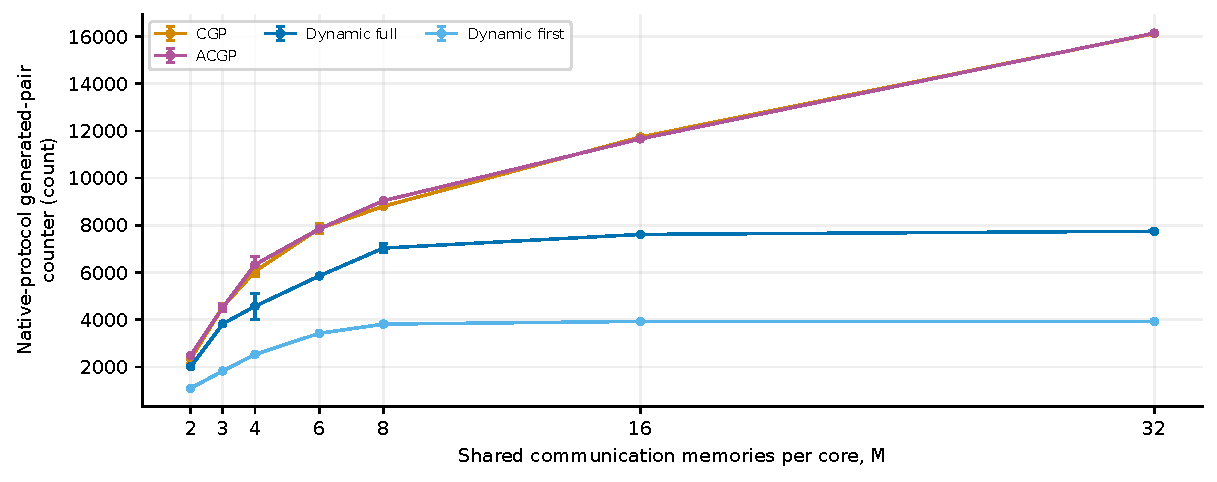
\includegraphics[width=.94\linewidth,height=.255\textheight,keepaspectratio]{figures/memory/mesh_yx_protocol_generated_pairs.pdf}\captionof{figure}{Run-level mean and sample SD. Shared trace aliases are counted once.}\end{center}
\begin{center}{\scriptsize\setlength{\tabcolsep}{3pt}
\begin{tabular}{lrrrrr}
\toprule
M & ODG & CGP & ACGP & Dynamic full & Dynamic first \\
\midrule
2 & n/a & $2337.00\pm173.95$ & $2485.00\pm38.18$ & $2010.00\pm48.08$ & $1099.00\pm21.21$ \\
3 & n/a & $4547.00\pm120.21$ & $4517.00\pm185.26$ & $3828.00\pm14.14$ & $1831.00\pm9.90$ \\
4 & n/a & $6046.00\pm197.99$ & $6333.00\pm357.80$ & $4570.00\pm560.03$ & $2534.00\pm5.66$ \\
6 & n/a & $7864.00\pm214.96$ & $7850.00\pm5.66$ & $5855.00\pm32.53$ & $3426.00\pm28.28$ \\
8 & n/a & $8806.00\pm31.11$ & $9042.00\pm70.71$ & $7037.00\pm199.40$ & $3816.00\pm73.54$ \\
16 & n/a & $11741.00\pm55.15$ & $11663.00\pm1.41$ & $7616.00\pm33.94$ & $3930.00\pm0.00$ \\
32 & n/a & $16125.00\pm52.33$ & $16142.00\pm25.46$ & $7752.00\pm0.00$ & $3930.00\pm0.00$ \\
\bottomrule\end{tabular}}
\captionof{table}{Mean $\pm$ sample SD; n/a denotes a metric outside that policy's instrumentation.}
{\footnotesize\href{https://github.com/sanjeevkrishnaa/Compiler-Driven-ACE/blob/codex/ace-scheduler-correctness/docs/latex/qft96_final/data/memory_mesh_yx_protocol_generated_pairs.csv}{Exact CSV values and sample counts}}
\end{center}
\clearpage
\subsection*{Native-protocol used-pair counter}
\begin{center}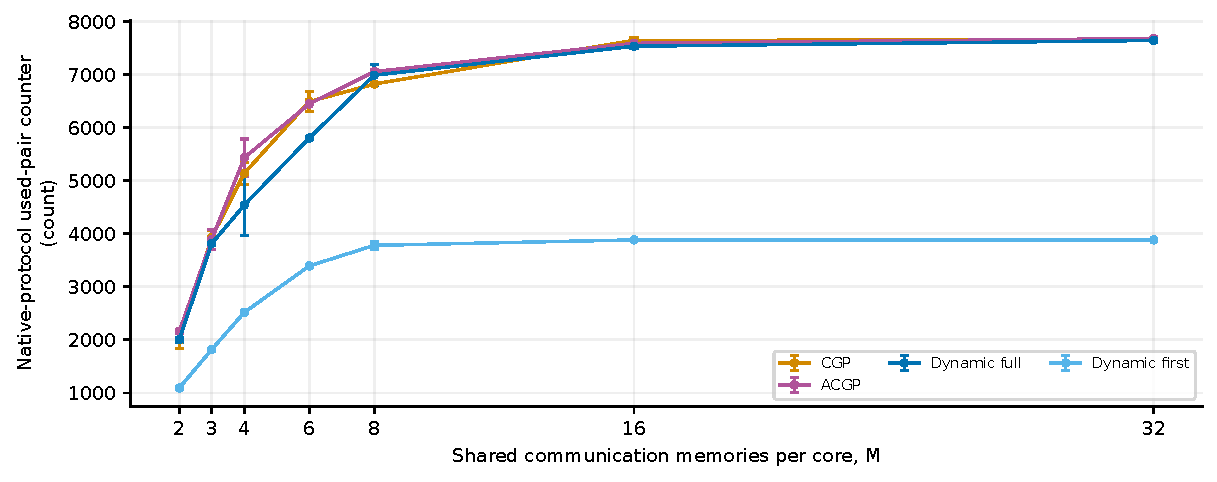
\includegraphics[width=.94\linewidth,height=.255\textheight,keepaspectratio]{figures/memory/mesh_yx_protocol_used_pairs.pdf}\captionof{figure}{Run-level mean and sample SD. Shared trace aliases are counted once.}\end{center}
\begin{center}{\scriptsize\setlength{\tabcolsep}{3pt}
\begin{tabular}{lrrrrr}
\toprule
M & ODG & CGP & ACGP & Dynamic full & Dynamic first \\
\midrule
2 & n/a & $1998.00\pm169.71$ & $2159.00\pm38.18$ & $2004.00\pm48.08$ & $1092.00\pm19.80$ \\
3 & n/a & $3930.00\pm132.94$ & $3895.00\pm185.26$ & $3816.00\pm11.31$ & $1819.00\pm9.90$ \\
4 & n/a & $5140.00\pm206.48$ & $5435.00\pm352.14$ & $4540.00\pm568.51$ & $2516.00\pm5.66$ \\
6 & n/a & $6492.00\pm192.33$ & $6448.00\pm14.14$ & $5805.00\pm32.53$ & $3393.00\pm32.53$ \\
8 & n/a & $6823.00\pm9.90$ & $7057.00\pm38.18$ & $6990.00\pm197.99$ & $3781.00\pm80.61$ \\
16 & n/a & $7648.00\pm48.08$ & $7591.00\pm7.07$ & $7536.00\pm33.94$ & $3884.00\pm8.49$ \\
32 & n/a & $7651.00\pm12.73$ & $7681.00\pm12.73$ & $7645.00\pm9.90$ & $3884.00\pm8.49$ \\
\bottomrule\end{tabular}}
\captionof{table}{Mean $\pm$ sample SD; n/a denotes a metric outside that policy's instrumentation.}
{\footnotesize\href{https://github.com/sanjeevkrishnaa/Compiler-Driven-ACE/blob/codex/ace-scheduler-correctness/docs/latex/qft96_final/data/memory_mesh_yx_protocol_used_pairs.csv}{Exact CSV values and sample counts}}
\end{center}
\subsection*{Native-protocol unused-pair counter}
\begin{center}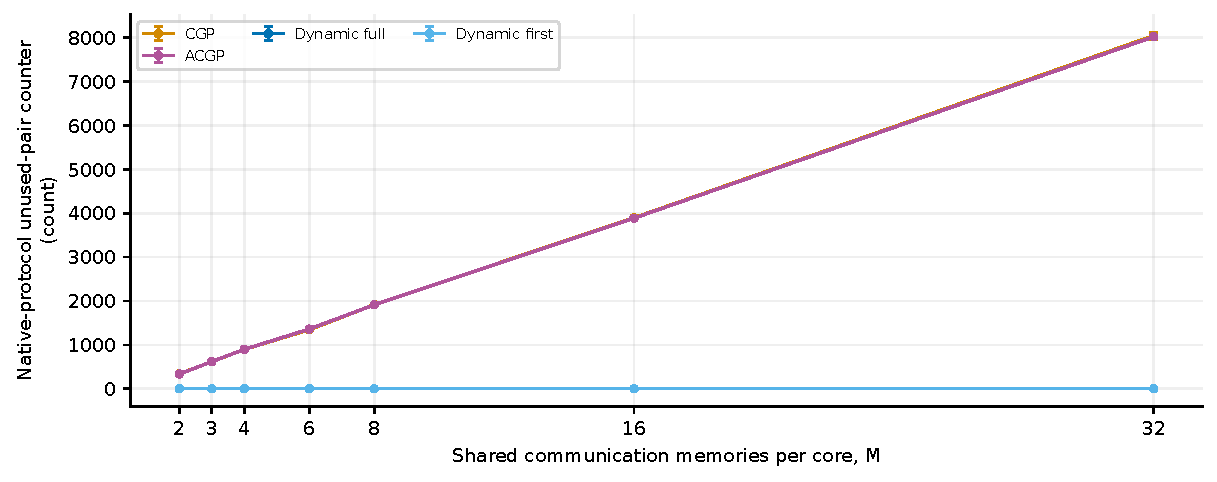
\includegraphics[width=.94\linewidth,height=.255\textheight,keepaspectratio]{figures/memory/mesh_yx_protocol_unused_pairs.pdf}\captionof{figure}{Run-level mean and sample SD. Shared trace aliases are counted once.}\end{center}
\begin{center}{\scriptsize\setlength{\tabcolsep}{3pt}
\begin{tabular}{lrrrrr}
\toprule
M & ODG & CGP & ACGP & Dynamic full & Dynamic first \\
\midrule
2 & n/a & $340.00\pm2.83$ & $335.00\pm1.41$ & $0.0000\pm0.0000$ & $0.0000\pm0.0000$ \\
3 & n/a & $617.00\pm7.07$ & $618.00\pm8.49$ & $0.0000\pm0.0000$ & $0.0000\pm0.0000$ \\
4 & n/a & $898.00\pm8.49$ & $897.00\pm1.41$ & $0.0000\pm0.0000$ & $0.0000\pm0.0000$ \\
6 & n/a & $1344.00\pm19.80$ & $1360.00\pm8.49$ & $0.0000\pm0.0000$ & $0.0000\pm0.0000$ \\
8 & n/a & $1916.00\pm5.66$ & $1914.00\pm19.80$ & $0.0000\pm0.0000$ & $0.0000\pm0.0000$ \\
16 & n/a & $3896.00\pm0.00$ & $3888.00\pm8.49$ & $0.0000\pm0.0000$ & $0.0000\pm0.0000$ \\
32 & n/a & $8048.00\pm76.37$ & $8025.00\pm46.67$ & $0.0000\pm0.0000$ & $0.0000\pm0.0000$ \\
\bottomrule\end{tabular}}
\captionof{table}{Mean $\pm$ sample SD; n/a denotes a metric outside that policy's instrumentation.}
{\footnotesize\href{https://github.com/sanjeevkrishnaa/Compiler-Driven-ACE/blob/codex/ace-scheduler-correctness/docs/latex/qft96_final/data/memory_mesh_yx_protocol_unused_pairs.csv}{Exact CSV values and sample counts}}
\end{center}
\clearpage
\subsection*{Scheduled compiler preparations}
\begin{center}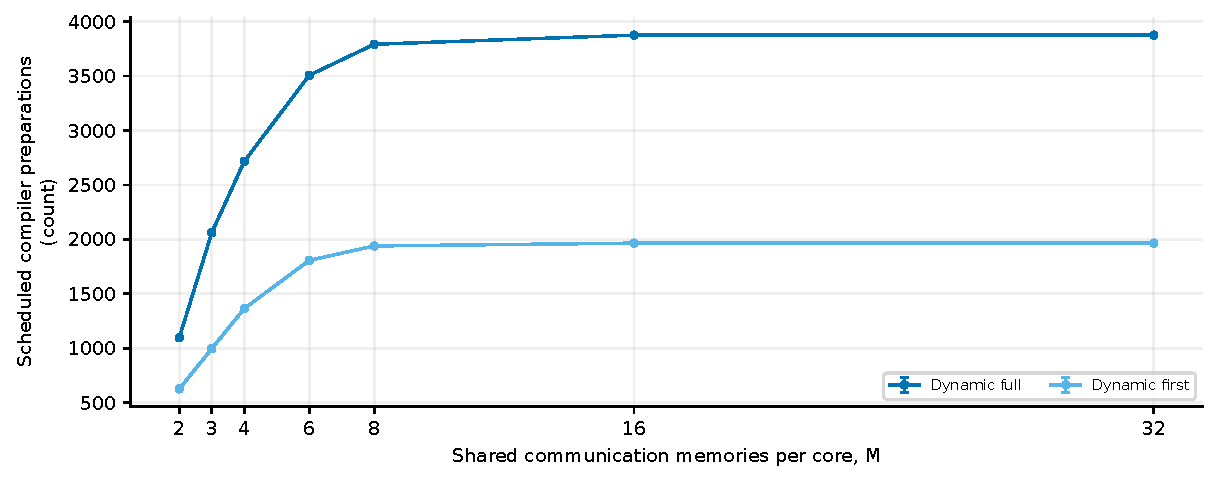
\includegraphics[width=.94\linewidth,height=.255\textheight,keepaspectratio]{figures/memory/mesh_yx_scheduled_preparations.pdf}\captionof{figure}{Run-level mean and sample SD. Shared trace aliases are counted once.}\end{center}
\begin{center}{\scriptsize\setlength{\tabcolsep}{3pt}
\begin{tabular}{lrrrrr}
\toprule
M & ODG & CGP & ACGP & Dynamic full & Dynamic first \\
\midrule
2 & n/a & n/a & n/a & $1097.00\pm0.00$ & $626.00\pm0.00$ \\
3 & n/a & n/a & n/a & $2062.00\pm0.00$ & $996.00\pm0.00$ \\
4 & n/a & n/a & n/a & $2716.00\pm0.00$ & $1364.00\pm0.00$ \\
6 & n/a & n/a & n/a & $3507.00\pm0.00$ & $1807.00\pm0.00$ \\
8 & n/a & n/a & n/a & $3792.00\pm0.00$ & $1939.00\pm0.00$ \\
16 & n/a & n/a & n/a & $3876.00\pm0.00$ & $1965.00\pm0.00$ \\
32 & n/a & n/a & n/a & $3876.00\pm0.00$ & $1965.00\pm0.00$ \\
\bottomrule\end{tabular}}
\captionof{table}{Mean $\pm$ sample SD; n/a denotes a metric outside that policy's instrumentation.}
{\footnotesize\href{https://github.com/sanjeevkrishnaa/Compiler-Driven-ACE/blob/codex/ace-scheduler-correctness/docs/latex/qft96_final/data/memory_mesh_yx_scheduled_preparations.csv}{Exact CSV values and sample counts}}
\end{center}
\subsection*{Planner-blocked preparations}
\begin{center}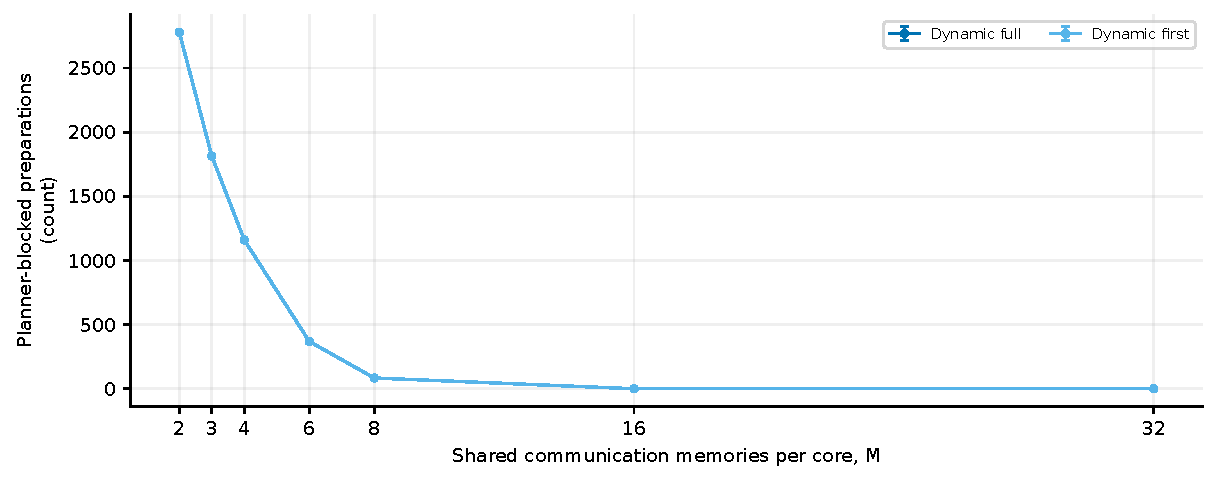
\includegraphics[width=.94\linewidth,height=.255\textheight,keepaspectratio]{figures/memory/mesh_yx_planner_blocked_preparations.pdf}\captionof{figure}{Run-level mean and sample SD. Shared trace aliases are counted once.}\end{center}
\begin{center}{\scriptsize\setlength{\tabcolsep}{3pt}
\begin{tabular}{lrrrrr}
\toprule
M & ODG & CGP & ACGP & Dynamic full & Dynamic first \\
\midrule
2 & n/a & n/a & n/a & $2779.00\pm0.00$ & $2779.00\pm0.00$ \\
3 & n/a & n/a & n/a & $1814.00\pm0.00$ & $1814.00\pm0.00$ \\
4 & n/a & n/a & n/a & $1160.00\pm0.00$ & $1160.00\pm0.00$ \\
6 & n/a & n/a & n/a & $369.00\pm0.00$ & $369.00\pm0.00$ \\
8 & n/a & n/a & n/a & $84.000\pm0.000$ & $84.000\pm0.000$ \\
16 & n/a & n/a & n/a & $0.0000\pm0.0000$ & $0.0000\pm0.0000$ \\
32 & n/a & n/a & n/a & $0.0000\pm0.0000$ & $0.0000\pm0.0000$ \\
\bottomrule\end{tabular}}
\captionof{table}{Mean $\pm$ sample SD; n/a denotes a metric outside that policy's instrumentation.}
{\footnotesize\href{https://github.com/sanjeevkrishnaa/Compiler-Driven-ACE/blob/codex/ace-scheduler-correctness/docs/latex/qft96_final/data/memory_mesh_yx_planner_blocked_preparations.csv}{Exact CSV values and sample counts}}
\end{center}
\clearpage
\subsection*{Planner peak compiler memory}
\begin{center}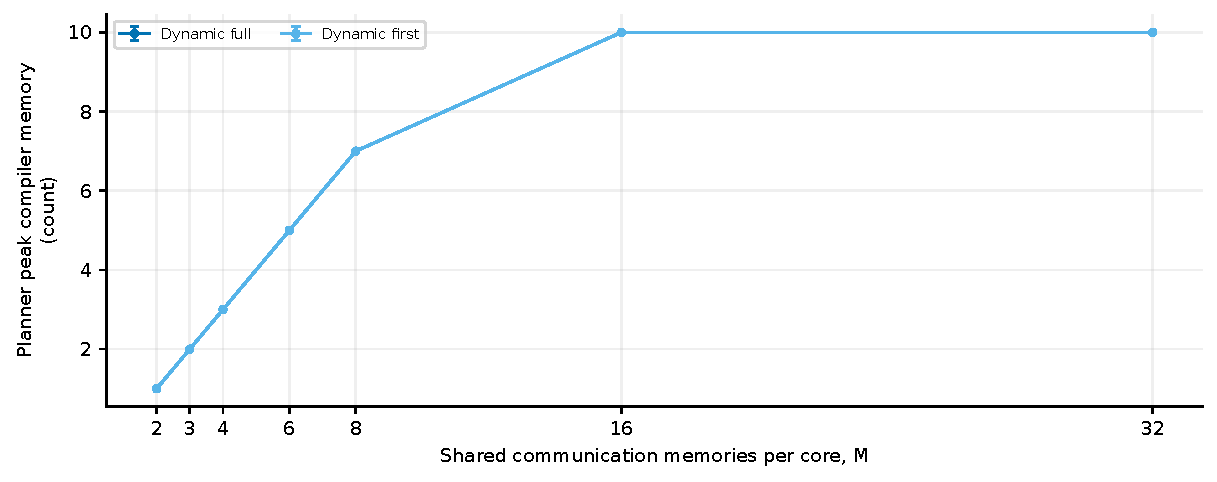
\includegraphics[width=.94\linewidth,height=.255\textheight,keepaspectratio]{figures/memory/mesh_yx_planner_peak_compiler_memory_per_core.pdf}\captionof{figure}{Run-level mean and sample SD. Shared trace aliases are counted once.}\end{center}
\begin{center}{\scriptsize\setlength{\tabcolsep}{3pt}
\begin{tabular}{lrrrrr}
\toprule
M & ODG & CGP & ACGP & Dynamic full & Dynamic first \\
\midrule
2 & n/a & n/a & n/a & $1.000\pm0.000$ & $1.000\pm0.000$ \\
3 & n/a & n/a & n/a & $2.000\pm0.000$ & $2.000\pm0.000$ \\
4 & n/a & n/a & n/a & $3.000\pm0.000$ & $3.000\pm0.000$ \\
6 & n/a & n/a & n/a & $5.000\pm0.000$ & $5.000\pm0.000$ \\
8 & n/a & n/a & n/a & $7.000\pm0.000$ & $7.000\pm0.000$ \\
16 & n/a & n/a & n/a & $10.000\pm0.000$ & $10.000\pm0.000$ \\
32 & n/a & n/a & n/a & $10.000\pm0.000$ & $10.000\pm0.000$ \\
\bottomrule\end{tabular}}
\captionof{table}{Mean $\pm$ sample SD; n/a denotes a metric outside that policy's instrumentation.}
{\footnotesize\href{https://github.com/sanjeevkrishnaa/Compiler-Driven-ACE/blob/codex/ace-scheduler-correctness/docs/latex/qft96_final/data/memory_mesh_yx_planner_peak_compiler_memory_per_core.csv}{Exact CSV values and sample counts}}
\end{center}
\subsection*{Compiler preparation admission attempts}
\begin{center}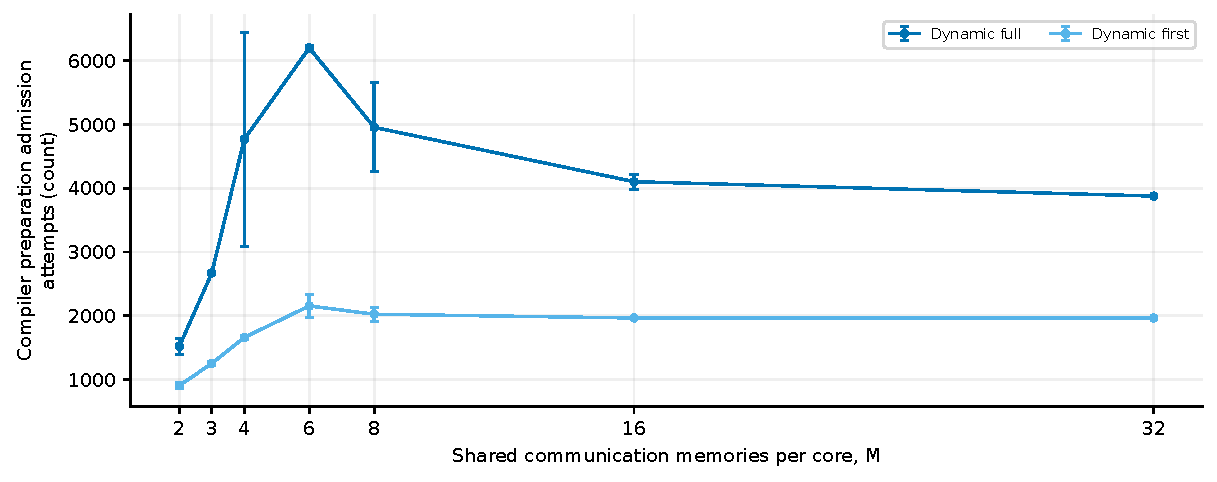
\includegraphics[width=.94\linewidth,height=.255\textheight,keepaspectratio]{figures/memory/mesh_yx_runtime_admission_attempts.pdf}\captionof{figure}{Run-level mean and sample SD. Shared trace aliases are counted once.}\end{center}
\begin{center}{\scriptsize\setlength{\tabcolsep}{3pt}
\begin{tabular}{lrrrrr}
\toprule
M & ODG & CGP & ACGP & Dynamic full & Dynamic first \\
\midrule
2 & n/a & n/a & n/a & $1519.50\pm125.16$ & $907.50\pm51.62$ \\
3 & n/a & n/a & n/a & $2670.50\pm26.16$ & $1251.50\pm34.65$ \\
4 & n/a & n/a & n/a & $4766.50\pm1676.55$ & $1659.50\pm27.58$ \\
6 & n/a & n/a & n/a & $6198.50\pm40.31$ & $2154.00\pm185.26$ \\
8 & n/a & n/a & n/a & $4953.50\pm697.91$ & $2024.00\pm111.72$ \\
16 & n/a & n/a & n/a & $4102.00\pm118.79$ & $1965.00\pm0.00$ \\
32 & n/a & n/a & n/a & $3876.00\pm0.00$ & $1965.00\pm0.00$ \\
\bottomrule\end{tabular}}
\captionof{table}{Mean $\pm$ sample SD; n/a denotes a metric outside that policy's instrumentation.}
{\footnotesize\href{https://github.com/sanjeevkrishnaa/Compiler-Driven-ACE/blob/codex/ace-scheduler-correctness/docs/latex/qft96_final/data/memory_mesh_yx_runtime_admission_attempts.csv}{Exact CSV values and sample counts}}
\end{center}
\clearpage
\subsection*{Launched compiler preparations}
\begin{center}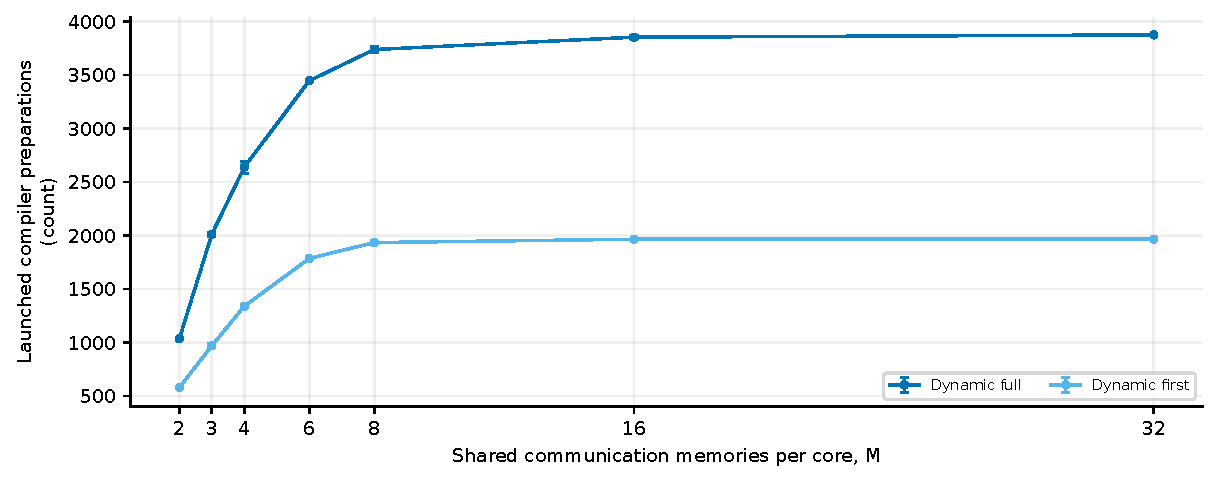
\includegraphics[width=.94\linewidth,height=.255\textheight,keepaspectratio]{figures/memory/mesh_yx_runtime_launched_preparations.pdf}\captionof{figure}{Run-level mean and sample SD. Shared trace aliases are counted once.}\end{center}
\begin{center}{\scriptsize\setlength{\tabcolsep}{3pt}
\begin{tabular}{lrrrrr}
\toprule
M & ODG & CGP & ACGP & Dynamic full & Dynamic first \\
\midrule
2 & n/a & n/a & n/a & $1035.00\pm2.83$ & $578.00\pm12.73$ \\
3 & n/a & n/a & n/a & $2010.50\pm19.09$ & $968.00\pm16.97$ \\
4 & n/a & n/a & n/a & $2639.00\pm55.15$ & $1338.00\pm7.07$ \\
6 & n/a & n/a & n/a & $3447.00\pm1.41$ & $1785.00\pm9.90$ \\
8 & n/a & n/a & n/a & $3739.00\pm24.04$ & $1933.50\pm6.36$ \\
16 & n/a & n/a & n/a & $3854.50\pm16.26$ & $1965.00\pm0.00$ \\
32 & n/a & n/a & n/a & $3876.00\pm0.00$ & $1965.00\pm0.00$ \\
\bottomrule\end{tabular}}
\captionof{table}{Mean $\pm$ sample SD; n/a denotes a metric outside that policy's instrumentation.}
{\footnotesize\href{https://github.com/sanjeevkrishnaa/Compiler-Driven-ACE/blob/codex/ace-scheduler-correctness/docs/latex/qft96_final/data/memory_mesh_yx_runtime_launched_preparations.csv}{Exact CSV values and sample counts}}
\end{center}
\subsection*{Accepted compiler preparations}
\begin{center}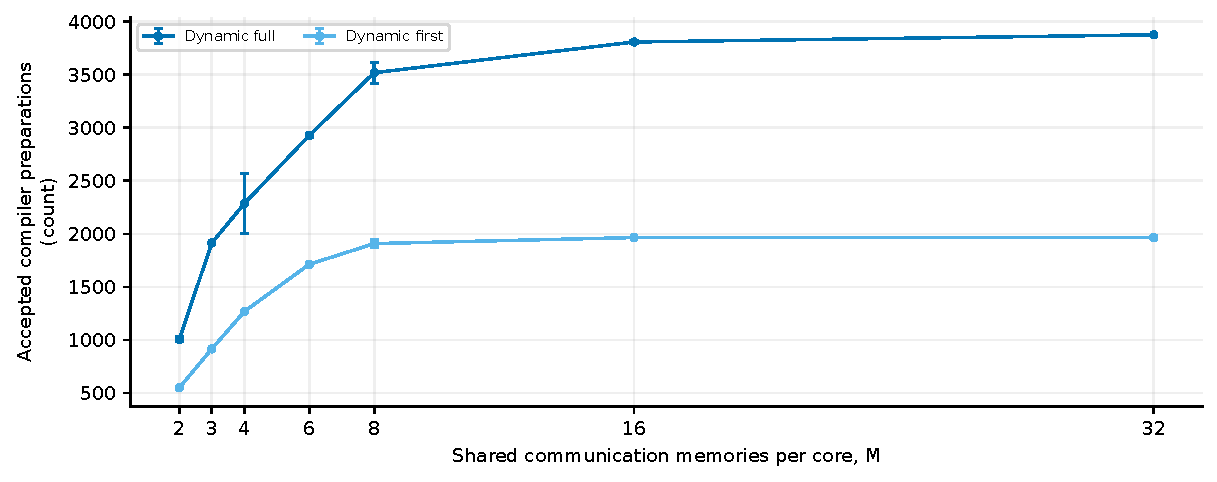
\includegraphics[width=.94\linewidth,height=.255\textheight,keepaspectratio]{figures/memory/mesh_yx_runtime_accepted_preparations.pdf}\captionof{figure}{Run-level mean and sample SD. Shared trace aliases are counted once.}\end{center}
\begin{center}{\scriptsize\setlength{\tabcolsep}{3pt}
\begin{tabular}{lrrrrr}
\toprule
M & ODG & CGP & ACGP & Dynamic full & Dynamic first \\
\midrule
2 & n/a & n/a & n/a & $1005.00\pm24.04$ & $549.50\pm10.61$ \\
3 & n/a & n/a & n/a & $1914.00\pm7.07$ & $915.50\pm4.95$ \\
4 & n/a & n/a & n/a & $2285.00\pm280.01$ & $1267.00\pm2.83$ \\
6 & n/a & n/a & n/a & $2927.50\pm16.26$ & $1713.00\pm14.14$ \\
8 & n/a & n/a & n/a & $3518.50\pm99.70$ & $1908.00\pm36.77$ \\
16 & n/a & n/a & n/a & $3808.00\pm16.97$ & $1965.00\pm0.00$ \\
32 & n/a & n/a & n/a & $3876.00\pm0.00$ & $1965.00\pm0.00$ \\
\bottomrule\end{tabular}}
\captionof{table}{Mean $\pm$ sample SD; n/a denotes a metric outside that policy's instrumentation.}
{\footnotesize\href{https://github.com/sanjeevkrishnaa/Compiler-Driven-ACE/blob/codex/ace-scheduler-correctness/docs/latex/qft96_final/data/memory_mesh_yx_runtime_accepted_preparations.csv}{Exact CSV values and sample counts}}
\end{center}
\clearpage
\subsection*{Rejected compiler preparations}
\begin{center}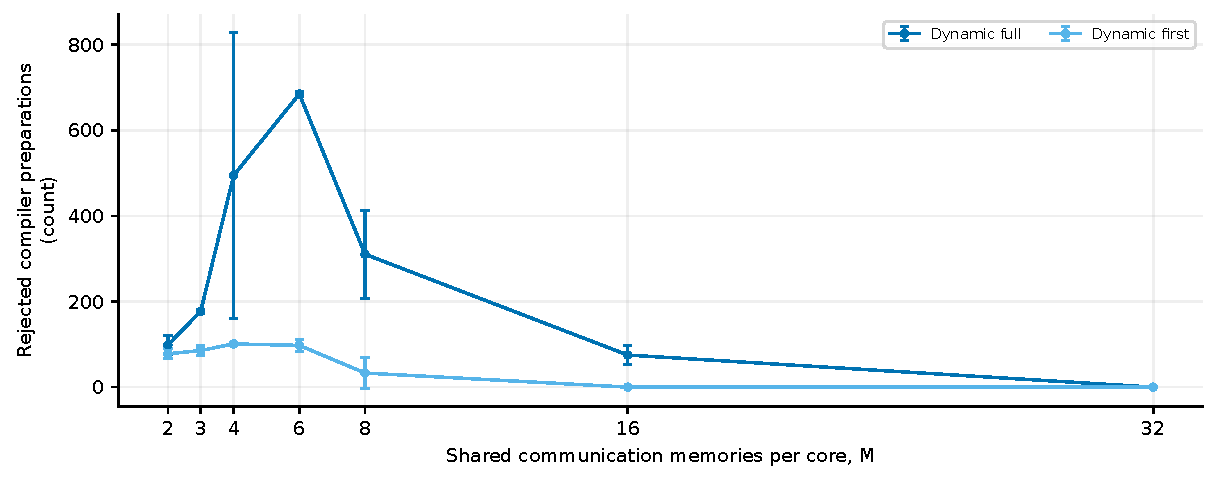
\includegraphics[width=.94\linewidth,height=.255\textheight,keepaspectratio]{figures/memory/mesh_yx_runtime_rejected_preparations.pdf}\captionof{figure}{Run-level mean and sample SD. Shared trace aliases are counted once.}\end{center}
\begin{center}{\scriptsize\setlength{\tabcolsep}{3pt}
\begin{tabular}{lrrrrr}
\toprule
M & ODG & CGP & ACGP & Dynamic full & Dynamic first \\
\midrule
2 & n/a & n/a & n/a & $98.500\pm21.920$ & $78.000\pm11.314$ \\
3 & n/a & n/a & n/a & $177.50\pm4.95$ & $85.500\pm10.607$ \\
4 & n/a & n/a & n/a & $494.50\pm334.46$ & $101.00\pm4.24$ \\
6 & n/a & n/a & n/a & $685.00\pm5.66$ & $97.500\pm14.849$ \\
8 & n/a & n/a & n/a & $310.50\pm102.53$ & $33.000\pm36.770$ \\
16 & n/a & n/a & n/a & $75.000\pm22.627$ & $0.0000\pm0.0000$ \\
32 & n/a & n/a & n/a & $0.0000\pm0.0000$ & $0.0000\pm0.0000$ \\
\bottomrule\end{tabular}}
\captionof{table}{Mean $\pm$ sample SD; n/a denotes a metric outside that policy's instrumentation.}
{\footnotesize\href{https://github.com/sanjeevkrishnaa/Compiler-Driven-ACE/blob/codex/ace-scheduler-correctness/docs/latex/qft96_final/data/memory_mesh_yx_runtime_rejected_preparations.csv}{Exact CSV values and sample counts}}
\end{center}
\subsection*{Compiler-ready request count}
\begin{center}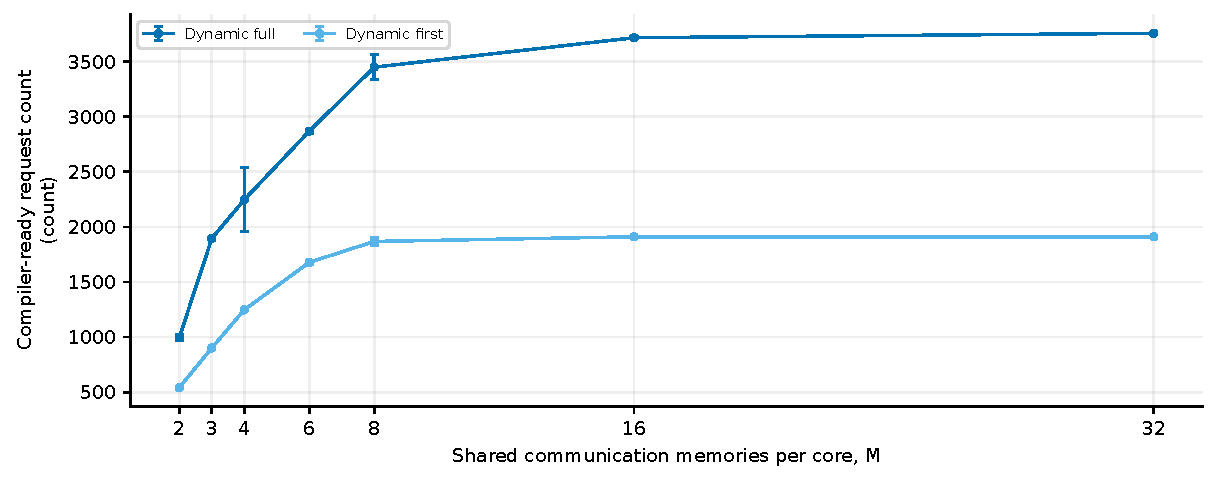
\includegraphics[width=.94\linewidth,height=.255\textheight,keepaspectratio]{figures/memory/mesh_yx_pregenerated_hits.pdf}\captionof{figure}{Run-level mean and sample SD. Shared trace aliases are counted once.}\end{center}
\begin{center}{\scriptsize\setlength{\tabcolsep}{3pt}
\begin{tabular}{lrrrrr}
\toprule
M & ODG & CGP & ACGP & Dynamic full & Dynamic first \\
\midrule
2 & n/a & n/a & n/a & $996.50\pm23.33$ & $542.00\pm9.90$ \\
3 & n/a & n/a & n/a & $1895.00\pm1.41$ & $902.50\pm2.12$ \\
4 & n/a & n/a & n/a & $2246.00\pm291.33$ & $1247.50\pm7.78$ \\
6 & n/a & n/a & n/a & $2867.00\pm16.97$ & $1678.00\pm16.97$ \\
8 & n/a & n/a & n/a & $3447.50\pm112.43$ & $1867.50\pm37.48$ \\
16 & n/a & n/a & n/a & $3714.50\pm10.61$ & $1910.00\pm4.24$ \\
32 & n/a & n/a & n/a & $3755.00\pm8.49$ & $1910.00\pm4.24$ \\
\bottomrule\end{tabular}}
\captionof{table}{Mean $\pm$ sample SD; n/a denotes a metric outside that policy's instrumentation.}
{\footnotesize\href{https://github.com/sanjeevkrishnaa/Compiler-Driven-ACE/blob/codex/ace-scheduler-correctness/docs/latex/qft96_final/data/memory_mesh_yx_pregenerated_hits.csv}{Exact CSV values and sample counts}}
\end{center}
\clearpage
\subsection*{Intended compiler-hit count}
\begin{center}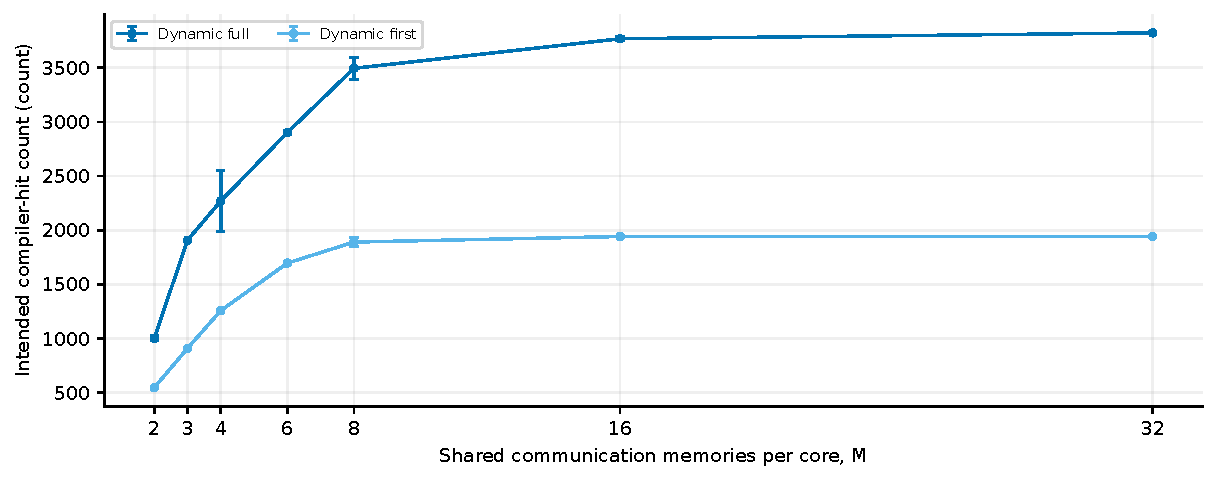
\includegraphics[width=.94\linewidth,height=.255\textheight,keepaspectratio]{figures/memory/mesh_yx_intended_request_hits.pdf}\captionof{figure}{Run-level mean and sample SD. Shared trace aliases are counted once.}\end{center}
\begin{center}{\scriptsize\setlength{\tabcolsep}{3pt}
\begin{tabular}{lrrrrr}
\toprule
M & ODG & CGP & ACGP & Dynamic full & Dynamic first \\
\midrule
2 & n/a & n/a & n/a & $1002.00\pm24.04$ & $546.00\pm9.90$ \\
3 & n/a & n/a & n/a & $1908.00\pm5.66$ & $909.50\pm4.95$ \\
4 & n/a & n/a & n/a & $2270.00\pm284.26$ & $1258.00\pm2.83$ \\
6 & n/a & n/a & n/a & $2902.50\pm16.26$ & $1696.50\pm16.26$ \\
8 & n/a & n/a & n/a & $3495.00\pm98.99$ & $1890.50\pm40.31$ \\
16 & n/a & n/a & n/a & $3768.00\pm16.97$ & $1942.00\pm4.24$ \\
32 & n/a & n/a & n/a & $3822.50\pm4.95$ & $1942.00\pm4.24$ \\
\bottomrule\end{tabular}}
\captionof{table}{Mean $\pm$ sample SD; n/a denotes a metric outside that policy's instrumentation.}
{\footnotesize\href{https://github.com/sanjeevkrishnaa/Compiler-Driven-ACE/blob/codex/ace-scheduler-correctness/docs/latex/qft96_final/data/memory_mesh_yx_intended_request_hits.csv}{Exact CSV values and sample counts}}
\end{center}
\subsection*{Compiler-not-ready request count}
\begin{center}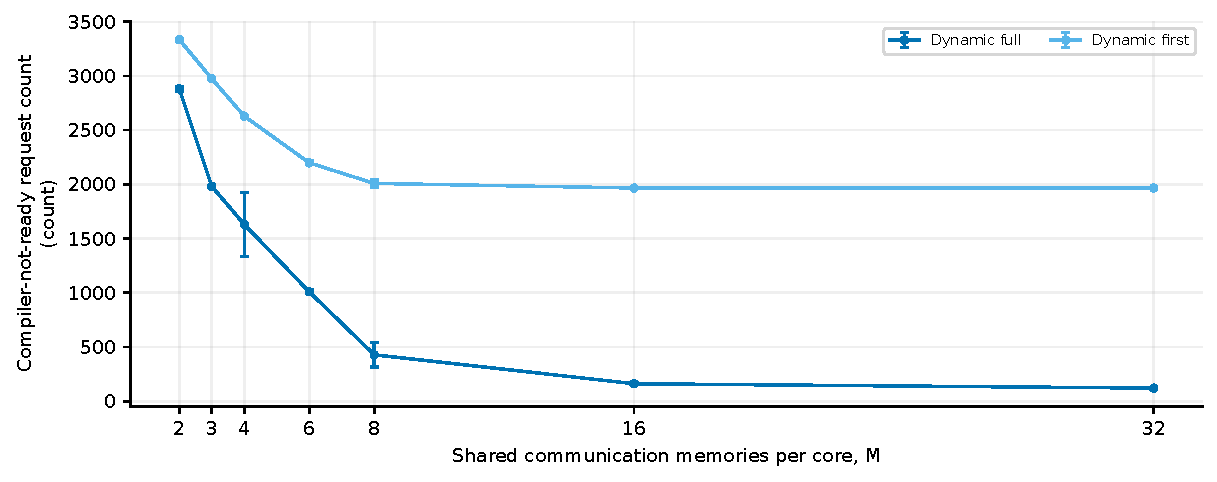
\includegraphics[width=.94\linewidth,height=.255\textheight,keepaspectratio]{figures/memory/mesh_yx_compiler_not_ready_requests.pdf}\captionof{figure}{Run-level mean and sample SD. Shared trace aliases are counted once.}\end{center}
\begin{center}{\scriptsize\setlength{\tabcolsep}{3pt}
\begin{tabular}{lrrrrr}
\toprule
M & ODG & CGP & ACGP & Dynamic full & Dynamic first \\
\midrule
2 & n/a & n/a & n/a & $2879.50\pm23.33$ & $3334.00\pm9.90$ \\
3 & n/a & n/a & n/a & $1981.00\pm1.41$ & $2973.50\pm2.12$ \\
4 & n/a & n/a & n/a & $1630.00\pm291.33$ & $2628.50\pm7.78$ \\
6 & n/a & n/a & n/a & $1009.00\pm16.97$ & $2198.00\pm16.97$ \\
8 & n/a & n/a & n/a & $428.50\pm112.43$ & $2008.50\pm37.48$ \\
16 & n/a & n/a & n/a & $161.50\pm10.61$ & $1966.00\pm4.24$ \\
32 & n/a & n/a & n/a & $121.00\pm8.49$ & $1966.00\pm4.24$ \\
\bottomrule\end{tabular}}
\captionof{table}{Mean $\pm$ sample SD; n/a denotes a metric outside that policy's instrumentation.}
{\footnotesize\href{https://github.com/sanjeevkrishnaa/Compiler-Driven-ACE/blob/codex/ace-scheduler-correctness/docs/latex/qft96_final/data/memory_mesh_yx_compiler_not_ready_requests.csv}{Exact CSV values and sample counts}}
\end{center}
\clearpage
\subsection*{Late compiler-pair uses}
\begin{center}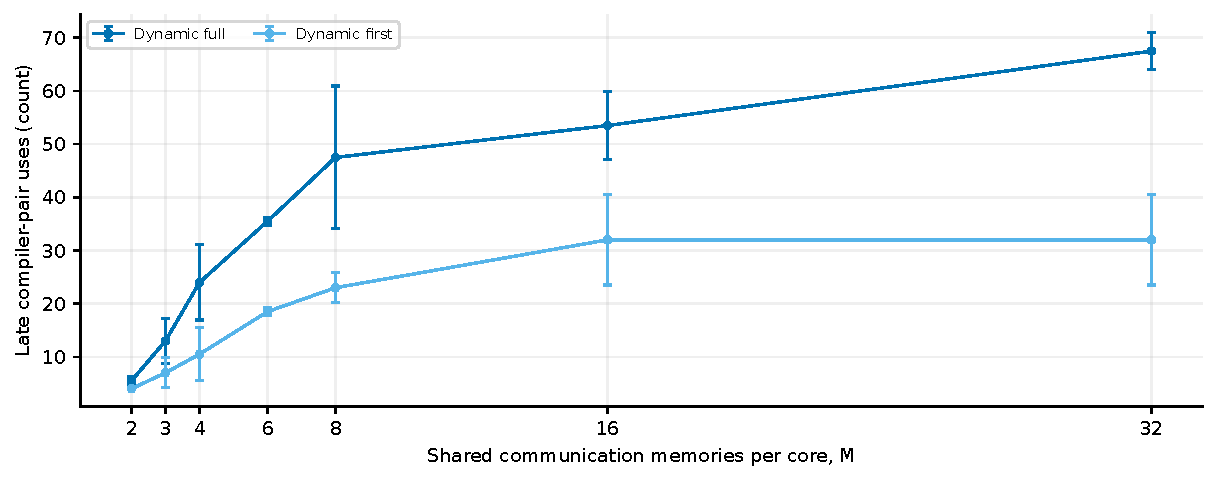
\includegraphics[width=.94\linewidth,height=.255\textheight,keepaspectratio]{figures/memory/mesh_yx_late_compiler_pair_uses.pdf}\captionof{figure}{Run-level mean and sample SD. Shared trace aliases are counted once.}\end{center}
\begin{center}{\scriptsize\setlength{\tabcolsep}{3pt}
\begin{tabular}{lrrrrr}
\toprule
M & ODG & CGP & ACGP & Dynamic full & Dynamic first \\
\midrule
2 & n/a & n/a & n/a & $5.500\pm0.707$ & $4.000\pm0.000$ \\
3 & n/a & n/a & n/a & $13.000\pm4.243$ & $7.000\pm2.828$ \\
4 & n/a & n/a & n/a & $24.000\pm7.071$ & $10.500\pm4.950$ \\
6 & n/a & n/a & n/a & $35.500\pm0.707$ & $18.500\pm0.707$ \\
8 & n/a & n/a & n/a & $47.500\pm13.435$ & $23.000\pm2.828$ \\
16 & n/a & n/a & n/a & $53.500\pm6.364$ & $32.000\pm8.485$ \\
32 & n/a & n/a & n/a & $67.500\pm3.536$ & $32.000\pm8.485$ \\
\bottomrule\end{tabular}}
\captionof{table}{Mean $\pm$ sample SD; n/a denotes a metric outside that policy's instrumentation.}
{\footnotesize\href{https://github.com/sanjeevkrishnaa/Compiler-Driven-ACE/blob/codex/ace-scheduler-correctness/docs/latex/qft96_final/data/memory_mesh_yx_late_compiler_pair_uses.csv}{Exact CSV values and sample counts}}
\end{center}
\subsection*{Compiler fallback count}
\begin{center}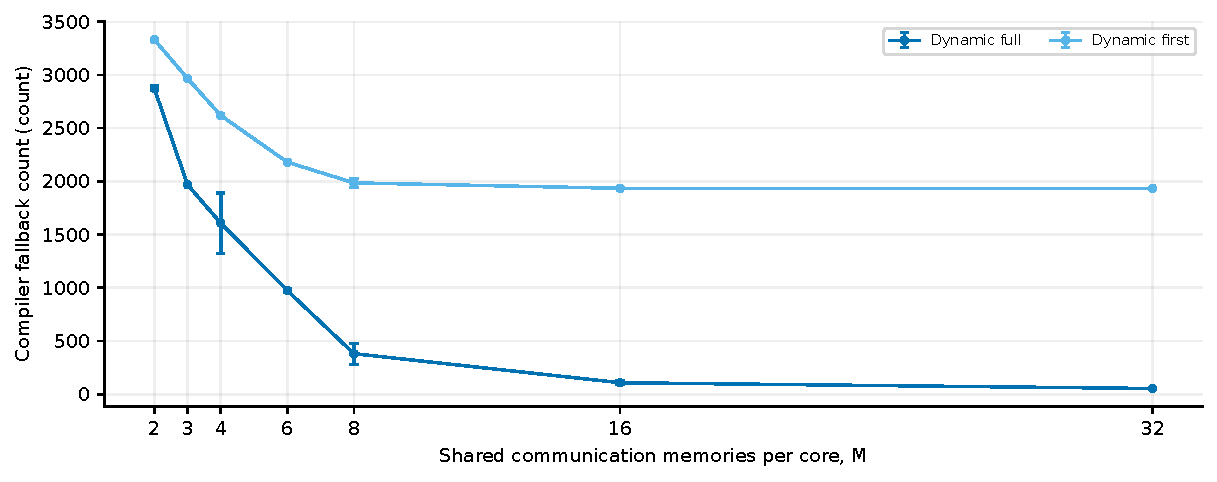
\includegraphics[width=.94\linewidth,height=.255\textheight,keepaspectratio]{figures/memory/mesh_yx_on_demand_fallbacks.pdf}\captionof{figure}{Run-level mean and sample SD. Shared trace aliases are counted once.}\end{center}
\begin{center}{\scriptsize\setlength{\tabcolsep}{3pt}
\begin{tabular}{lrrrrr}
\toprule
M & ODG & CGP & ACGP & Dynamic full & Dynamic first \\
\midrule
2 & n/a & n/a & n/a & $2874.00\pm24.04$ & $3330.00\pm9.90$ \\
3 & n/a & n/a & n/a & $1968.00\pm5.66$ & $2966.50\pm4.95$ \\
4 & n/a & n/a & n/a & $1606.00\pm284.26$ & $2618.00\pm2.83$ \\
6 & n/a & n/a & n/a & $973.50\pm16.26$ & $2179.50\pm16.26$ \\
8 & n/a & n/a & n/a & $381.00\pm98.99$ & $1985.50\pm40.31$ \\
16 & n/a & n/a & n/a & $108.00\pm16.97$ & $1934.00\pm4.24$ \\
32 & n/a & n/a & n/a & $53.500\pm4.950$ & $1934.00\pm4.24$ \\
\bottomrule\end{tabular}}
\captionof{table}{Mean $\pm$ sample SD; n/a denotes a metric outside that policy's instrumentation.}
{\footnotesize\href{https://github.com/sanjeevkrishnaa/Compiler-Driven-ACE/blob/codex/ace-scheduler-correctness/docs/latex/qft96_final/data/memory_mesh_yx_on_demand_fallbacks.csv}{Exact CSV values and sample counts}}
\end{center}
\clearpage
\subsection*{Generated compiler pairs}
\begin{center}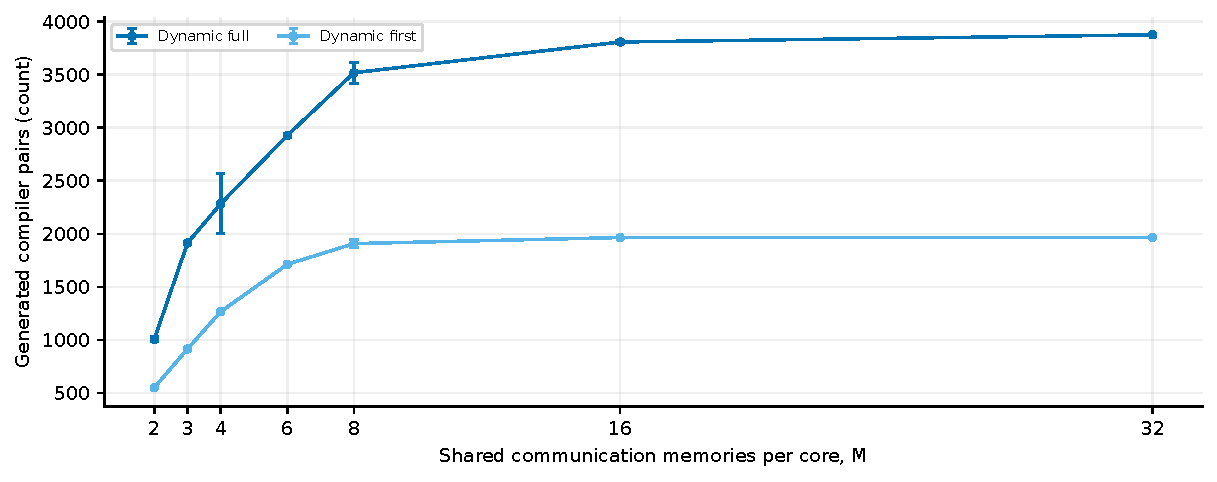
\includegraphics[width=.94\linewidth,height=.255\textheight,keepaspectratio]{figures/memory/mesh_yx_generated_compiler_pairs.pdf}\captionof{figure}{Run-level mean and sample SD. Shared trace aliases are counted once.}\end{center}
\begin{center}{\scriptsize\setlength{\tabcolsep}{3pt}
\begin{tabular}{lrrrrr}
\toprule
M & ODG & CGP & ACGP & Dynamic full & Dynamic first \\
\midrule
2 & n/a & n/a & n/a & $1005.00\pm24.04$ & $549.50\pm10.61$ \\
3 & n/a & n/a & n/a & $1914.00\pm7.07$ & $915.50\pm4.95$ \\
4 & n/a & n/a & n/a & $2285.00\pm280.01$ & $1267.00\pm2.83$ \\
6 & n/a & n/a & n/a & $2927.50\pm16.26$ & $1713.00\pm14.14$ \\
8 & n/a & n/a & n/a & $3518.50\pm99.70$ & $1908.00\pm36.77$ \\
16 & n/a & n/a & n/a & $3808.00\pm16.97$ & $1965.00\pm0.00$ \\
32 & n/a & n/a & n/a & $3876.00\pm0.00$ & $1965.00\pm0.00$ \\
\bottomrule\end{tabular}}
\captionof{table}{Mean $\pm$ sample SD; n/a denotes a metric outside that policy's instrumentation.}
{\footnotesize\href{https://github.com/sanjeevkrishnaa/Compiler-Driven-ACE/blob/codex/ace-scheduler-correctness/docs/latex/qft96_final/data/memory_mesh_yx_generated_compiler_pairs.csv}{Exact CSV values and sample counts}}
\end{center}
\subsection*{Used compiler pairs}
\begin{center}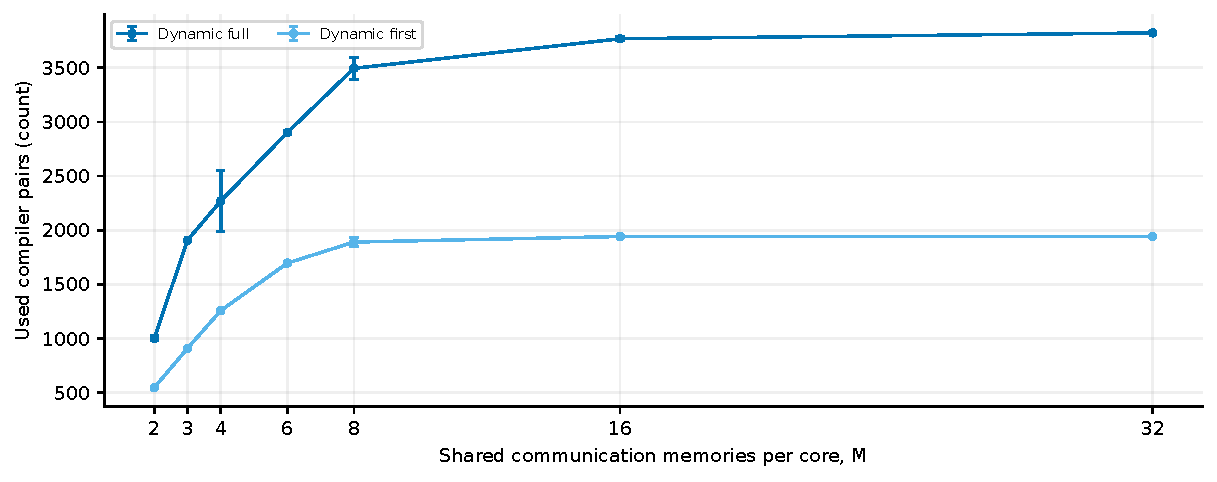
\includegraphics[width=.94\linewidth,height=.255\textheight,keepaspectratio]{figures/memory/mesh_yx_utilized_compiler_pairs.pdf}\captionof{figure}{Run-level mean and sample SD. Shared trace aliases are counted once.}\end{center}
\begin{center}{\scriptsize\setlength{\tabcolsep}{3pt}
\begin{tabular}{lrrrrr}
\toprule
M & ODG & CGP & ACGP & Dynamic full & Dynamic first \\
\midrule
2 & n/a & n/a & n/a & $1002.00\pm24.04$ & $546.00\pm9.90$ \\
3 & n/a & n/a & n/a & $1908.00\pm5.66$ & $909.50\pm4.95$ \\
4 & n/a & n/a & n/a & $2270.00\pm284.26$ & $1258.00\pm2.83$ \\
6 & n/a & n/a & n/a & $2902.50\pm16.26$ & $1696.50\pm16.26$ \\
8 & n/a & n/a & n/a & $3495.00\pm98.99$ & $1890.50\pm40.31$ \\
16 & n/a & n/a & n/a & $3768.00\pm16.97$ & $1942.00\pm4.24$ \\
32 & n/a & n/a & n/a & $3822.50\pm4.95$ & $1942.00\pm4.24$ \\
\bottomrule\end{tabular}}
\captionof{table}{Mean $\pm$ sample SD; n/a denotes a metric outside that policy's instrumentation.}
{\footnotesize\href{https://github.com/sanjeevkrishnaa/Compiler-Driven-ACE/blob/codex/ace-scheduler-correctness/docs/latex/qft96_final/data/memory_mesh_yx_utilized_compiler_pairs.csv}{Exact CSV values and sample counts}}
\end{center}
\clearpage
\subsection*{Expired compiler pairs}
\begin{center}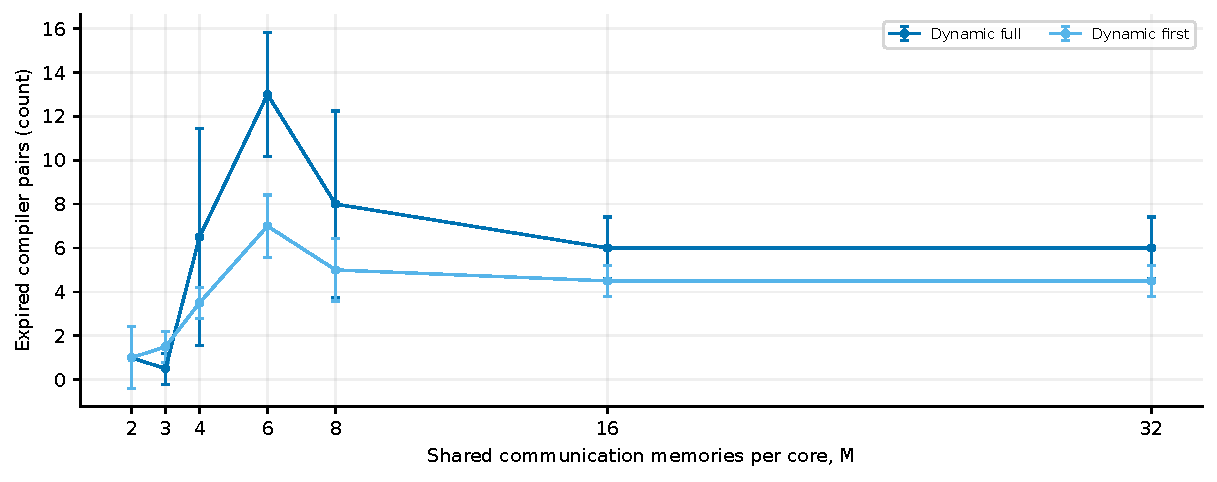
\includegraphics[width=.94\linewidth,height=.255\textheight,keepaspectratio]{figures/memory/mesh_yx_expired_compiler_pairs.pdf}\captionof{figure}{Run-level mean and sample SD. Shared trace aliases are counted once.}\end{center}
\begin{center}{\scriptsize\setlength{\tabcolsep}{3pt}
\begin{tabular}{lrrrrr}
\toprule
M & ODG & CGP & ACGP & Dynamic full & Dynamic first \\
\midrule
2 & n/a & n/a & n/a & $1.000\pm1.414$ & $1.000\pm1.414$ \\
3 & n/a & n/a & n/a & $0.5000\pm0.7071$ & $1.500\pm0.707$ \\
4 & n/a & n/a & n/a & $6.500\pm4.950$ & $3.500\pm0.707$ \\
6 & n/a & n/a & n/a & $13.000\pm2.828$ & $7.000\pm1.414$ \\
8 & n/a & n/a & n/a & $8.000\pm4.243$ & $5.000\pm1.414$ \\
16 & n/a & n/a & n/a & $6.000\pm1.414$ & $4.500\pm0.707$ \\
32 & n/a & n/a & n/a & $6.000\pm1.414$ & $4.500\pm0.707$ \\
\bottomrule\end{tabular}}
\captionof{table}{Mean $\pm$ sample SD; n/a denotes a metric outside that policy's instrumentation.}
{\footnotesize\href{https://github.com/sanjeevkrishnaa/Compiler-Driven-ACE/blob/codex/ace-scheduler-correctness/docs/latex/qft96_final/data/memory_mesh_yx_expired_compiler_pairs.csv}{Exact CSV values and sample counts}}
\end{center}
\subsection*{Remaining compiler pairs}
\begin{center}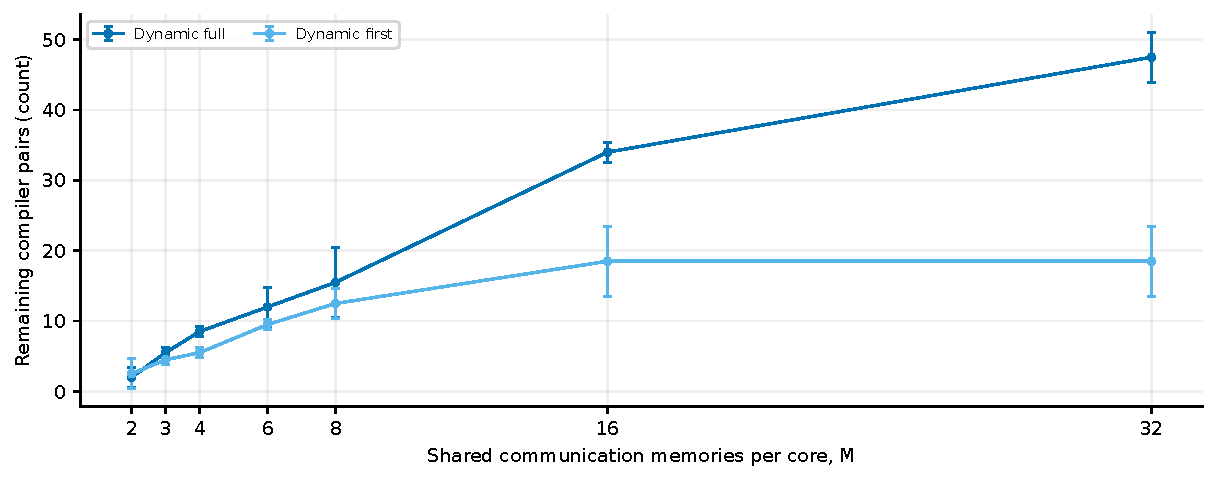
\includegraphics[width=.94\linewidth,height=.255\textheight,keepaspectratio]{figures/memory/mesh_yx_remaining_compiler_pairs.pdf}\captionof{figure}{Run-level mean and sample SD. Shared trace aliases are counted once.}\end{center}
\begin{center}{\scriptsize\setlength{\tabcolsep}{3pt}
\begin{tabular}{lrrrrr}
\toprule
M & ODG & CGP & ACGP & Dynamic full & Dynamic first \\
\midrule
2 & n/a & n/a & n/a & $2.000\pm1.414$ & $2.500\pm2.121$ \\
3 & n/a & n/a & n/a & $5.500\pm0.707$ & $4.500\pm0.707$ \\
4 & n/a & n/a & n/a & $8.500\pm0.707$ & $5.500\pm0.707$ \\
6 & n/a & n/a & n/a & $12.000\pm2.828$ & $9.500\pm0.707$ \\
8 & n/a & n/a & n/a & $15.500\pm4.950$ & $12.500\pm2.121$ \\
16 & n/a & n/a & n/a & $34.000\pm1.414$ & $18.500\pm4.950$ \\
32 & n/a & n/a & n/a & $47.500\pm3.536$ & $18.500\pm4.950$ \\
\bottomrule\end{tabular}}
\captionof{table}{Mean $\pm$ sample SD; n/a denotes a metric outside that policy's instrumentation.}
{\footnotesize\href{https://github.com/sanjeevkrishnaa/Compiler-Driven-ACE/blob/codex/ace-scheduler-correctness/docs/latex/qft96_final/data/memory_mesh_yx_remaining_compiler_pairs.csv}{Exact CSV values and sample counts}}
\end{center}
\clearpage
\subsection*{Compiler fidelity at creation}
\begin{center}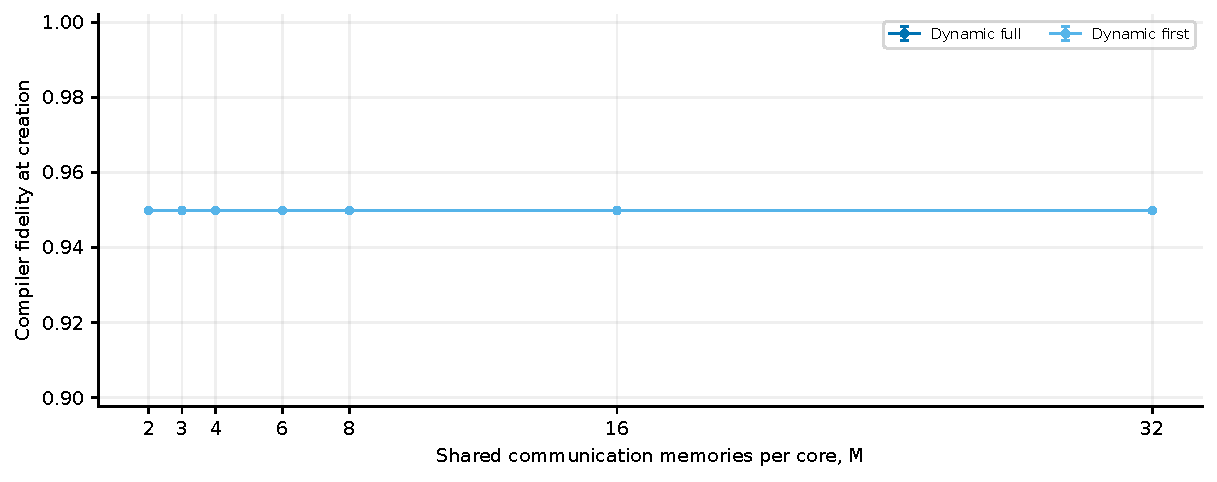
\includegraphics[width=.94\linewidth,height=.255\textheight,keepaspectratio]{figures/memory/mesh_yx_average_fidelity_at_creation.pdf}\captionof{figure}{Run-level mean and sample SD. Shared trace aliases are counted once.}\end{center}
\begin{center}{\scriptsize\setlength{\tabcolsep}{3pt}
\begin{tabular}{lrrrrr}
\toprule
M & ODG & CGP & ACGP & Dynamic full & Dynamic first \\
\midrule
2 & n/a & n/a & n/a & $0.9498\pm0.0000$ & $0.9498\pm0.0000$ \\
3 & n/a & n/a & n/a & $0.9498\pm0.0000$ & $0.9498\pm0.0000$ \\
4 & n/a & n/a & n/a & $0.9498\pm0.0000$ & $0.9498\pm0.0000$ \\
6 & n/a & n/a & n/a & $0.9498\pm0.0000$ & $0.9498\pm0.0000$ \\
8 & n/a & n/a & n/a & $0.9498\pm0.0000$ & $0.9498\pm0.0000$ \\
16 & n/a & n/a & n/a & $0.9498\pm0.0000$ & $0.9498\pm0.0000$ \\
32 & n/a & n/a & n/a & $0.9498\pm0.0000$ & $0.9498\pm0.0000$ \\
\bottomrule\end{tabular}}
\captionof{table}{Mean $\pm$ sample SD; n/a denotes a metric outside that policy's instrumentation.}
{\footnotesize\href{https://github.com/sanjeevkrishnaa/Compiler-Driven-ACE/blob/codex/ace-scheduler-correctness/docs/latex/qft96_final/data/memory_mesh_yx_average_fidelity_at_creation.csv}{Exact CSV values and sample counts}}
\end{center}
\subsection*{Compiler fidelity at use}
\begin{center}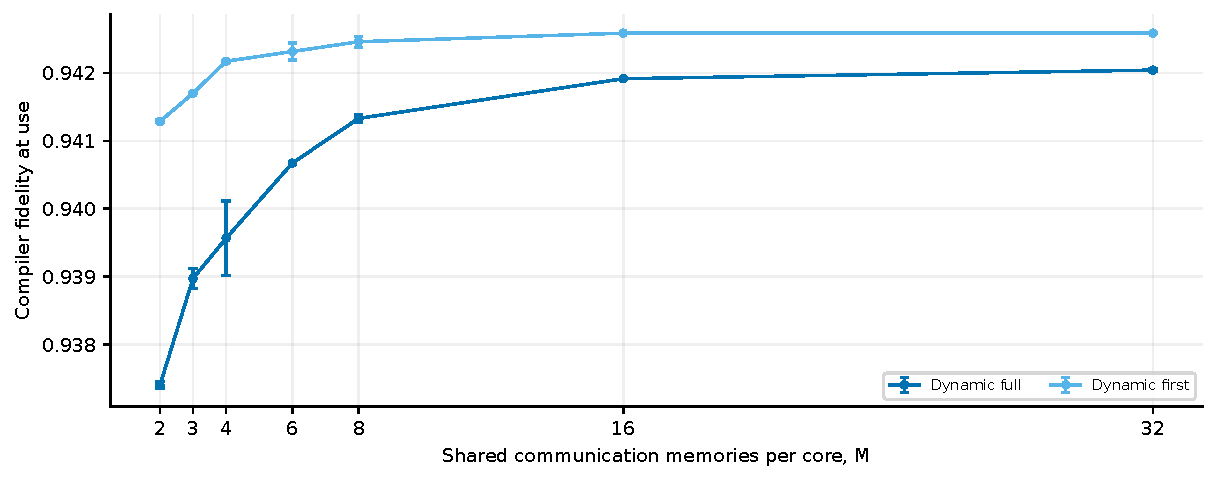
\includegraphics[width=.94\linewidth,height=.255\textheight,keepaspectratio]{figures/memory/mesh_yx_average_fidelity_at_utilization.pdf}\captionof{figure}{Run-level mean and sample SD. Shared trace aliases are counted once.}\end{center}
\begin{center}{\scriptsize\setlength{\tabcolsep}{3pt}
\begin{tabular}{lrrrrr}
\toprule
M & ODG & CGP & ACGP & Dynamic full & Dynamic first \\
\midrule
2 & n/a & n/a & n/a & $0.9374\pm0.0001$ & $0.9413\pm0.0000$ \\
3 & n/a & n/a & n/a & $0.9390\pm0.0001$ & $0.9417\pm0.0000$ \\
4 & n/a & n/a & n/a & $0.9396\pm0.0005$ & $0.9422\pm0.0000$ \\
6 & n/a & n/a & n/a & $0.9407\pm0.0000$ & $0.9423\pm0.0001$ \\
8 & n/a & n/a & n/a & $0.9413\pm0.0001$ & $0.9425\pm0.0001$ \\
16 & n/a & n/a & n/a & $0.9419\pm0.0000$ & $0.9426\pm0.0000$ \\
32 & n/a & n/a & n/a & $0.9420\pm0.0000$ & $0.9426\pm0.0000$ \\
\bottomrule\end{tabular}}
\captionof{table}{Mean $\pm$ sample SD; n/a denotes a metric outside that policy's instrumentation.}
{\footnotesize\href{https://github.com/sanjeevkrishnaa/Compiler-Driven-ACE/blob/codex/ace-scheduler-correctness/docs/latex/qft96_final/data/memory_mesh_yx_average_fidelity_at_utilization.csv}{Exact CSV values and sample counts}}
\end{center}
\clearpage
\subsection*{Mean layer latency}
\begin{center}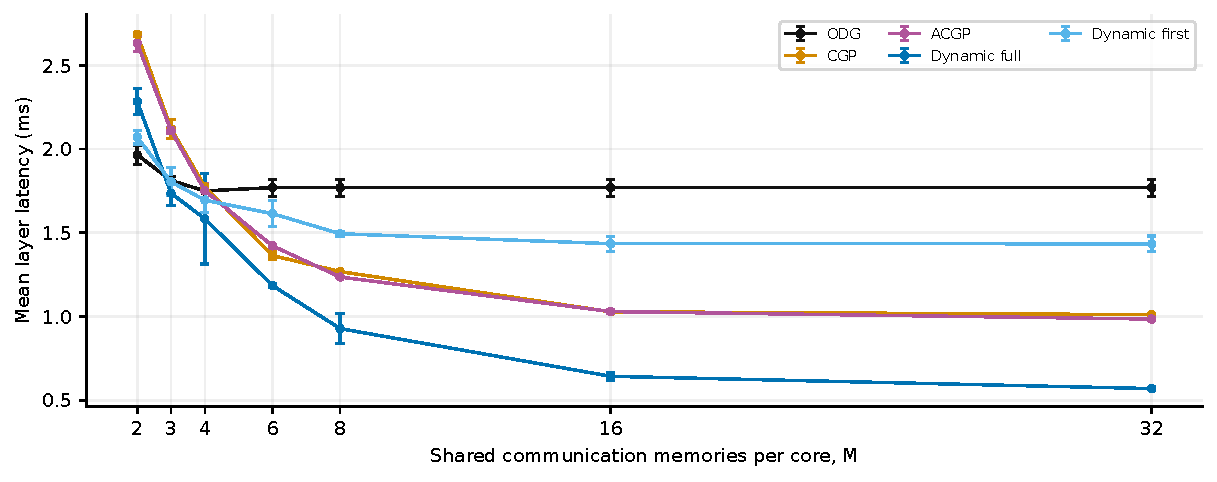
\includegraphics[width=.94\linewidth,height=.255\textheight,keepaspectratio]{figures/memory/mesh_yx_avg_layer_latency_ms.pdf}\captionof{figure}{Run-level mean and sample SD. Shared trace aliases are counted once.}\end{center}
\begin{center}{\scriptsize\setlength{\tabcolsep}{3pt}
\begin{tabular}{lrrrrr}
\toprule
M & ODG & CGP & ACGP & Dynamic full & Dynamic first \\
\midrule
2 & $1.966\pm0.057$ & $2.686\pm0.012$ & $2.632\pm0.047$ & $2.284\pm0.076$ & $2.072\pm0.042$ \\
3 & $1.812\pm0.023$ & $2.122\pm0.057$ & $2.111\pm0.017$ & $1.737\pm0.071$ & $1.805\pm0.084$ \\
4 & $1.750\pm0.042$ & $1.776\pm0.008$ & $1.751\pm0.042$ & $1.584\pm0.270$ & $1.695\pm0.076$ \\
6 & $1.770\pm0.051$ & $1.364\pm0.024$ & $1.422\pm0.008$ & $1.185\pm0.011$ & $1.614\pm0.078$ \\
8 & $1.770\pm0.051$ & $1.268\pm0.003$ & $1.236\pm0.005$ & $0.9278\pm0.0912$ & $1.495\pm0.014$ \\
16 & $1.770\pm0.051$ & $1.029\pm0.002$ & $1.029\pm0.010$ & $0.6428\pm0.0220$ & $1.435\pm0.046$ \\
32 & $1.770\pm0.051$ & $1.011\pm0.008$ & $0.9847\pm0.0091$ & $0.5693\pm0.0008$ & $1.434\pm0.046$ \\
\bottomrule\end{tabular}}
\captionof{table}{Mean $\pm$ sample SD; n/a denotes a metric outside that policy's instrumentation.}
{\footnotesize\href{https://github.com/sanjeevkrishnaa/Compiler-Driven-ACE/blob/codex/ace-scheduler-correctness/docs/latex/qft96_final/data/memory_mesh_yx_avg_layer_latency_ms.csv}{Exact CSV values and sample counts}}
\end{center}
\subsection*{Maximum layer latency}
\begin{center}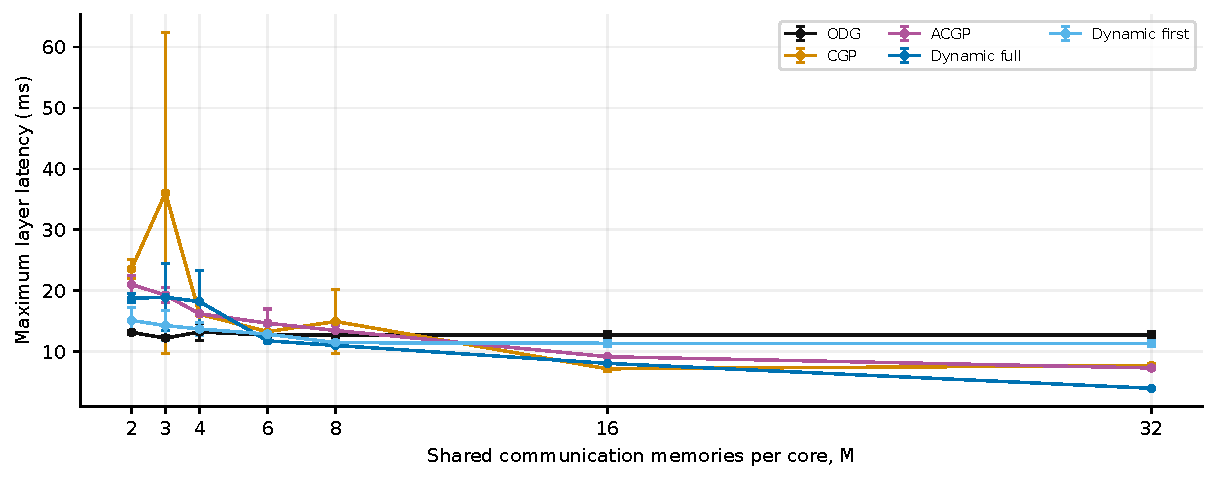
\includegraphics[width=.94\linewidth,height=.255\textheight,keepaspectratio]{figures/memory/mesh_yx_max_layer_latency_ms.pdf}\captionof{figure}{Run-level mean and sample SD. Shared trace aliases are counted once.}\end{center}
\begin{center}{\scriptsize\setlength{\tabcolsep}{3pt}
\begin{tabular}{lrrrrr}
\toprule
M & ODG & CGP & ACGP & Dynamic full & Dynamic first \\
\midrule
2 & $13.150\pm0.354$ & $23.551\pm1.626$ & $21.000\pm1.414$ & $18.750\pm0.778$ & $15.100\pm2.121$ \\
3 & $12.200\pm0.424$ & $36.050\pm26.375$ & $19.250\pm1.202$ & $18.900\pm5.516$ & $14.250\pm2.475$ \\
4 & $13.200\pm1.414$ & $16.150\pm0.212$ & $16.200\pm0.141$ & $18.200\pm5.091$ & $13.700\pm0.990$ \\
6 & $12.700\pm0.566$ & $13.250\pm0.212$ & $14.650\pm2.333$ & $11.750\pm0.212$ & $12.850\pm1.344$ \\
8 & $12.700\pm0.566$ & $14.932\pm5.188$ & $13.450\pm0.778$ & $11.000\pm0.141$ & $11.450\pm0.354$ \\
16 & $12.700\pm0.566$ & $7.150\pm0.495$ & $9.143\pm0.202$ & $8.050\pm1.202$ & $11.350\pm0.495$ \\
32 & $12.700\pm0.566$ & $7.700\pm0.283$ & $7.289\pm0.298$ & $3.950\pm0.071$ & $11.350\pm0.495$ \\
\bottomrule\end{tabular}}
\captionof{table}{Mean $\pm$ sample SD; n/a denotes a metric outside that policy's instrumentation.}
{\footnotesize\href{https://github.com/sanjeevkrishnaa/Compiler-Driven-ACE/blob/codex/ace-scheduler-correctness/docs/latex/qft96_final/data/memory_mesh_yx_max_layer_latency_ms.csv}{Exact CSV values and sample counts}}
\end{center}
\clearpage
\subsection*{Minimum layer latency}
\begin{center}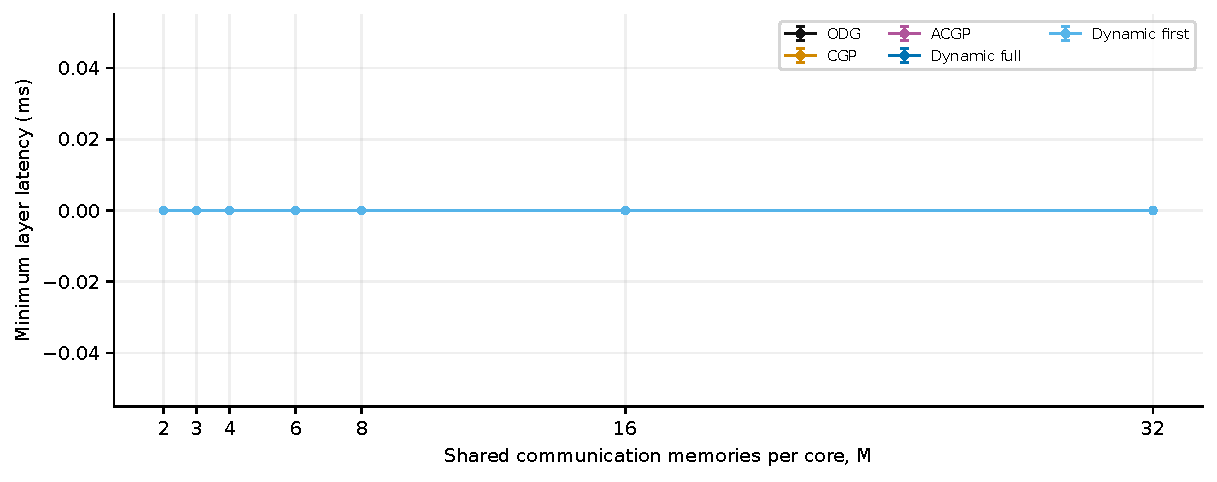
\includegraphics[width=.94\linewidth,height=.255\textheight,keepaspectratio]{figures/memory/mesh_yx_min_layer_latency_ms.pdf}\captionof{figure}{Run-level mean and sample SD. Shared trace aliases are counted once.}\end{center}
\begin{center}{\scriptsize\setlength{\tabcolsep}{3pt}
\begin{tabular}{lrrrrr}
\toprule
M & ODG & CGP & ACGP & Dynamic full & Dynamic first \\
\midrule
2 & $0.0000\pm0.0000$ & $0.0000\pm0.0000$ & $0.0000\pm0.0000$ & $0.0000\pm0.0000$ & $0.0000\pm0.0000$ \\
3 & $0.0000\pm0.0000$ & $0.0000\pm0.0000$ & $0.0000\pm0.0000$ & $0.0000\pm0.0000$ & $0.0000\pm0.0000$ \\
4 & $0.0000\pm0.0000$ & $0.0000\pm0.0000$ & $0.0000\pm0.0000$ & $0.0000\pm0.0000$ & $0.0000\pm0.0000$ \\
6 & $0.0000\pm0.0000$ & $0.0000\pm0.0000$ & $0.0000\pm0.0000$ & $0.0000\pm0.0000$ & $0.0000\pm0.0000$ \\
8 & $0.0000\pm0.0000$ & $0.0000\pm0.0000$ & $0.0000\pm0.0000$ & $0.0000\pm0.0000$ & $0.0000\pm0.0000$ \\
16 & $0.0000\pm0.0000$ & $0.0000\pm0.0000$ & $0.0000\pm0.0000$ & $0.0000\pm0.0000$ & $0.0000\pm0.0000$ \\
32 & $0.0000\pm0.0000$ & $0.0000\pm0.0000$ & $0.0000\pm0.0000$ & $0.0000\pm0.0000$ & $0.0000\pm0.0000$ \\
\bottomrule\end{tabular}}
\captionof{table}{Mean $\pm$ sample SD; n/a denotes a metric outside that policy's instrumentation.}
{\footnotesize\href{https://github.com/sanjeevkrishnaa/Compiler-Driven-ACE/blob/codex/ace-scheduler-correctness/docs/latex/qft96_final/data/memory_mesh_yx_min_layer_latency_ms.csv}{Exact CSV values and sample counts}}
\end{center}
\section{Shortest Reliable}
\clearpage
\subsection*{Mean request latency}
\begin{center}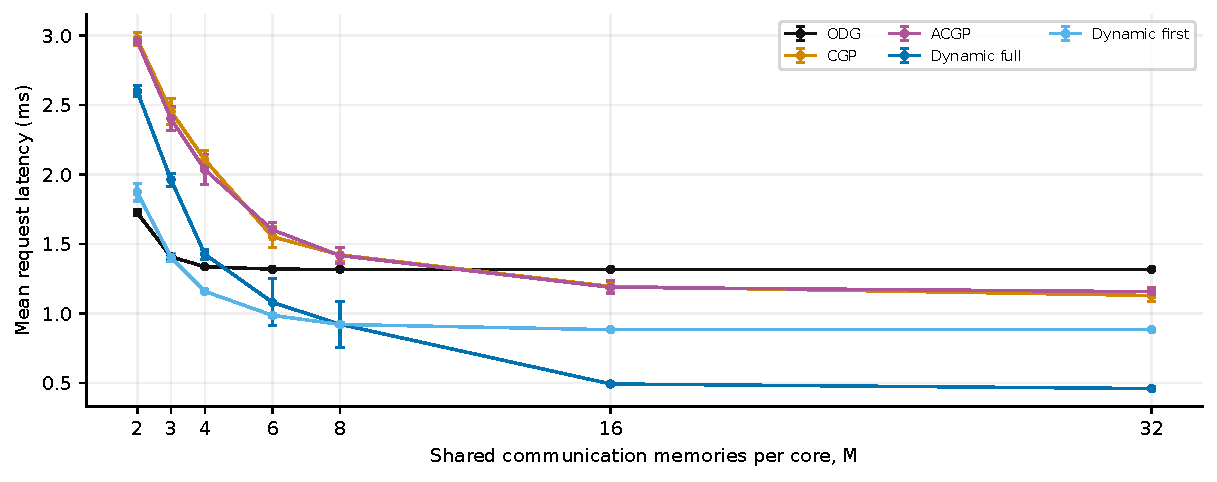
\includegraphics[width=.94\linewidth,height=.255\textheight,keepaspectratio]{figures/memory/mesh_shortest_reliable_request_latency_mean_ms.pdf}\captionof{figure}{Run-level mean and sample SD. Shared trace aliases are counted once.}\end{center}
\begin{center}{\scriptsize\setlength{\tabcolsep}{3pt}
\begin{tabular}{lrrrrr}
\toprule
M & ODG & CGP & ACGP & Dynamic full & Dynamic first \\
\midrule
2 & $1.726\pm0.022$ & $2.976\pm0.047$ & $2.959\pm0.027$ & $2.598\pm0.040$ & $1.872\pm0.062$ \\
3 & $1.408\pm0.010$ & $2.455\pm0.093$ & $2.401\pm0.085$ & $1.963\pm0.046$ & $1.405\pm0.028$ \\
4 & $1.337\pm0.005$ & $2.106\pm0.066$ & $2.035\pm0.109$ & $1.427\pm0.036$ & $1.160\pm0.010$ \\
6 & $1.319\pm0.004$ & $1.553\pm0.077$ & $1.602\pm0.053$ & $1.080\pm0.169$ & $0.9875\pm0.0125$ \\
8 & $1.319\pm0.004$ & $1.422\pm0.051$ & $1.417\pm0.059$ & $0.9230\pm0.1635$ & $0.9220\pm0.0102$ \\
16 & $1.318\pm0.004$ & $1.195\pm0.043$ & $1.189\pm0.046$ & $0.4941\pm0.0101$ & $0.8841\pm0.0083$ \\
32 & $1.318\pm0.004$ & $1.130\pm0.046$ & $1.157\pm0.030$ & $0.4607\pm0.0011$ & $0.8841\pm0.0083$ \\
\bottomrule\end{tabular}}
\captionof{table}{Mean $\pm$ sample SD; n/a denotes a metric outside that policy's instrumentation.}
{\footnotesize\href{https://github.com/sanjeevkrishnaa/Compiler-Driven-ACE/blob/codex/ace-scheduler-correctness/docs/latex/qft96_final/data/memory_mesh_shortest_reliable_request_latency_mean_ms.csv}{Exact CSV values and sample counts}}
\end{center}
\subsection*{Median request latency}
\begin{center}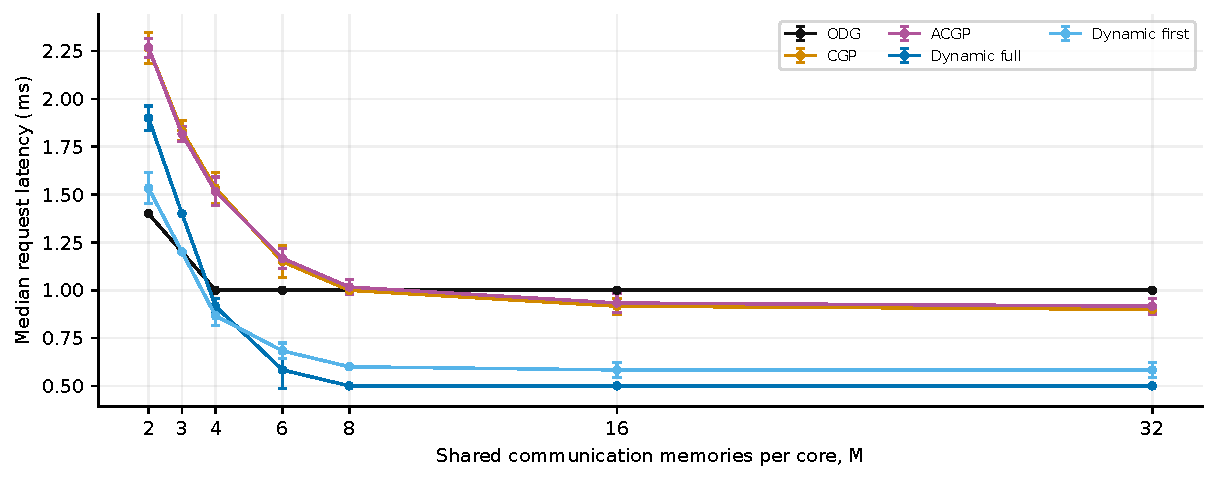
\includegraphics[width=.94\linewidth,height=.255\textheight,keepaspectratio]{figures/memory/mesh_shortest_reliable_request_latency_median_ms.pdf}\captionof{figure}{Run-level mean and sample SD. Shared trace aliases are counted once.}\end{center}
\begin{center}{\scriptsize\setlength{\tabcolsep}{3pt}
\begin{tabular}{lrrrrr}
\toprule
M & ODG & CGP & ACGP & Dynamic full & Dynamic first \\
\midrule
2 & $1.400\pm0.000$ & $2.267\pm0.082$ & $2.268\pm0.050$ & $1.900\pm0.063$ & $1.533\pm0.082$ \\
3 & $1.200\pm0.000$ & $1.833\pm0.052$ & $1.817\pm0.041$ & $1.400\pm0.000$ & $1.200\pm0.000$ \\
4 & $1.000\pm0.000$ & $1.533\pm0.082$ & $1.517\pm0.075$ & $0.9167\pm0.0408$ & $0.8667\pm0.0516$ \\
6 & $1.000\pm0.000$ & $1.150\pm0.084$ & $1.167\pm0.052$ & $0.5833\pm0.0983$ & $0.6833\pm0.0408$ \\
8 & $1.000\pm0.000$ & $1.000\pm0.000$ & $1.017\pm0.041$ & $0.5000\pm0.0000$ & $0.6000\pm0.0000$ \\
16 & $1.000\pm0.000$ & $0.9167\pm0.0408$ & $0.9333\pm0.0516$ & $0.5000\pm0.0000$ & $0.5833\pm0.0408$ \\
32 & $1.000\pm0.000$ & $0.9000\pm0.0000$ & $0.9167\pm0.0408$ & $0.5000\pm0.0000$ & $0.5833\pm0.0408$ \\
\bottomrule\end{tabular}}
\captionof{table}{Mean $\pm$ sample SD; n/a denotes a metric outside that policy's instrumentation.}
{\footnotesize\href{https://github.com/sanjeevkrishnaa/Compiler-Driven-ACE/blob/codex/ace-scheduler-correctness/docs/latex/qft96_final/data/memory_mesh_shortest_reliable_request_latency_median_ms.csv}{Exact CSV values and sample counts}}
\end{center}
\clearpage
\subsection*{p95 request latency}
\begin{center}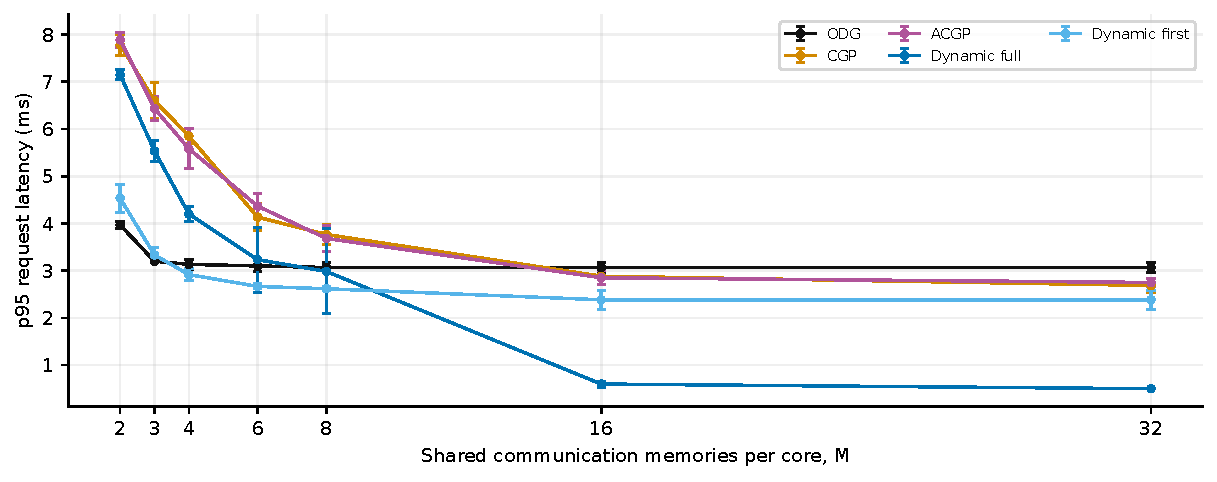
\includegraphics[width=.94\linewidth,height=.255\textheight,keepaspectratio]{figures/memory/mesh_shortest_reliable_request_latency_p95_ms.pdf}\captionof{figure}{Run-level mean and sample SD. Shared trace aliases are counted once.}\end{center}
\begin{center}{\scriptsize\setlength{\tabcolsep}{3pt}
\begin{tabular}{lrrrrr}
\toprule
M & ODG & CGP & ACGP & Dynamic full & Dynamic first \\
\midrule
2 & $3.967\pm0.082$ & $7.785\pm0.226$ & $7.886\pm0.161$ & $7.150\pm0.105$ & $4.533\pm0.294$ \\
3 & $3.200\pm0.000$ & $6.600\pm0.385$ & $6.433\pm0.258$ & $5.533\pm0.225$ & $3.333\pm0.163$ \\
4 & $3.133\pm0.103$ & $5.850\pm0.164$ & $5.581\pm0.424$ & $4.200\pm0.155$ & $2.917\pm0.133$ \\
6 & $3.100\pm0.110$ & $4.133\pm0.288$ & $4.367\pm0.258$ & $3.233\pm0.689$ & $2.667\pm0.052$ \\
8 & $3.067\pm0.103$ & $3.767\pm0.216$ & $3.683\pm0.279$ & $2.983\pm0.900$ & $2.617\pm0.041$ \\
16 & $3.067\pm0.103$ & $2.883\pm0.172$ & $2.850\pm0.152$ & $0.6000\pm0.0633$ & $2.383\pm0.204$ \\
32 & $3.067\pm0.103$ & $2.687\pm0.150$ & $2.750\pm0.084$ & $0.5000\pm0.0000$ & $2.383\pm0.204$ \\
\bottomrule\end{tabular}}
\captionof{table}{Mean $\pm$ sample SD; n/a denotes a metric outside that policy's instrumentation.}
{\footnotesize\href{https://github.com/sanjeevkrishnaa/Compiler-Driven-ACE/blob/codex/ace-scheduler-correctness/docs/latex/qft96_final/data/memory_mesh_shortest_reliable_request_latency_p95_ms.csv}{Exact CSV values and sample counts}}
\end{center}
\subsection*{Maximum request latency}
\begin{center}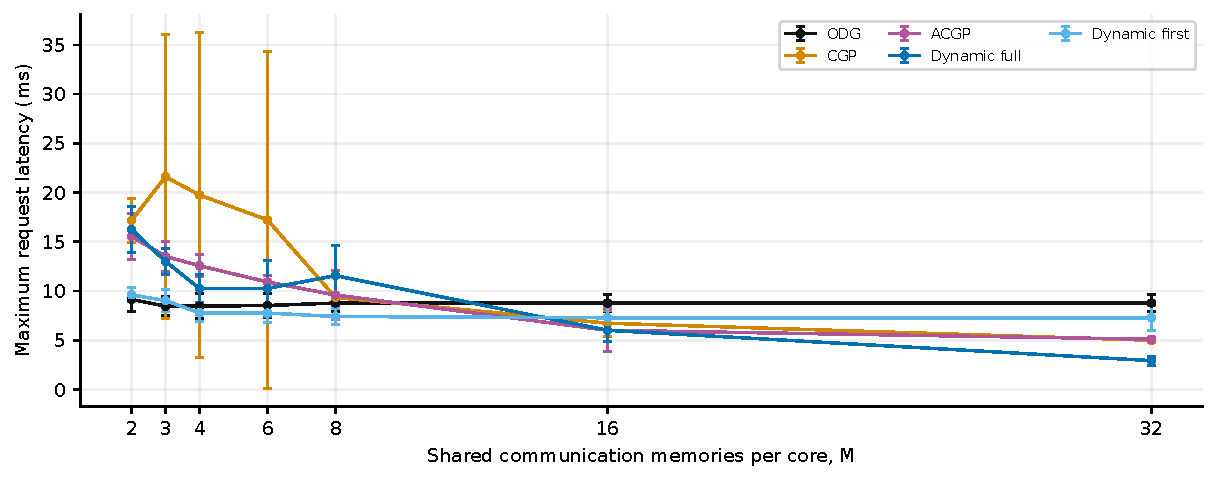
\includegraphics[width=.94\linewidth,height=.255\textheight,keepaspectratio]{figures/memory/mesh_shortest_reliable_request_latency_max_ms.pdf}\captionof{figure}{Run-level mean and sample SD. Shared trace aliases are counted once.}\end{center}
\begin{center}{\scriptsize\setlength{\tabcolsep}{3pt}
\begin{tabular}{lrrrrr}
\toprule
M & ODG & CGP & ACGP & Dynamic full & Dynamic first \\
\midrule
2 & $9.150\pm1.190$ & $17.166\pm2.216$ & $15.550\pm2.321$ & $16.250\pm2.318$ & $9.617\pm0.697$ \\
3 & $8.467\pm0.965$ & $21.600\pm14.422$ & $13.517\pm1.515$ & $13.017\pm1.332$ & $9.034\pm1.129$ \\
4 & $8.467\pm1.244$ & $19.750\pm16.521$ & $12.567\pm1.111$ & $10.250\pm1.429$ & $7.784\pm0.911$ \\
6 & $8.534\pm1.211$ & $17.224\pm17.144$ & $10.917\pm0.697$ & $10.267\pm2.813$ & $7.767\pm0.973$ \\
8 & $8.784\pm0.861$ & $9.347\pm2.058$ & $9.602\pm2.462$ & $11.567\pm3.089$ & $7.417\pm0.809$ \\
16 & $8.784\pm0.861$ & $6.733\pm1.332$ & $6.017\pm2.181$ & $6.017\pm1.155$ & $7.284\pm1.298$ \\
32 & $8.784\pm0.861$ & $5.000\pm0.179$ & $5.107\pm0.175$ & $2.933\pm0.463$ & $7.284\pm1.298$ \\
\bottomrule\end{tabular}}
\captionof{table}{Mean $\pm$ sample SD; n/a denotes a metric outside that policy's instrumentation.}
{\footnotesize\href{https://github.com/sanjeevkrishnaa/Compiler-Driven-ACE/blob/codex/ace-scheduler-correctness/docs/latex/qft96_final/data/memory_mesh_shortest_reliable_request_latency_max_ms.csv}{Exact CSV values and sample counts}}
\end{center}
\clearpage
\subsection*{Communication makespan}
\begin{center}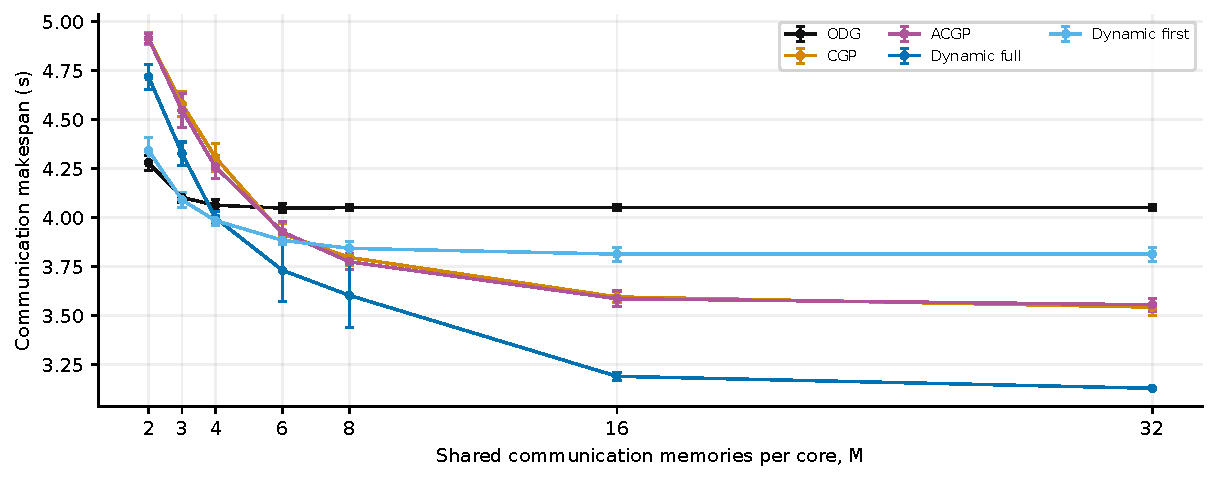
\includegraphics[width=.94\linewidth,height=.255\textheight,keepaspectratio]{figures/memory/mesh_shortest_reliable_end_to_end_latency_ms.pdf}\captionof{figure}{Run-level mean and sample SD. Shared trace aliases are counted once.}\end{center}
\begin{center}{\scriptsize\setlength{\tabcolsep}{3pt}
\begin{tabular}{lrrrrr}
\toprule
M & ODG & CGP & ACGP & Dynamic full & Dynamic first \\
\midrule
2 & $4.280\pm0.038$ & $4.914\pm0.031$ & $4.914\pm0.025$ & $4.718\pm0.063$ & $4.342\pm0.064$ \\
3 & $4.103\pm0.026$ & $4.580\pm0.065$ & $4.548\pm0.086$ & $4.327\pm0.059$ & $4.090\pm0.039$ \\
4 & $4.064\pm0.029$ & $4.307\pm0.070$ & $4.258\pm0.060$ & $3.998\pm0.031$ & $3.985\pm0.026$ \\
6 & $4.049\pm0.021$ & $3.917\pm0.052$ & $3.927\pm0.053$ & $3.731\pm0.161$ & $3.885\pm0.024$ \\
8 & $4.051\pm0.017$ & $3.797\pm0.039$ & $3.775\pm0.041$ & $3.604\pm0.165$ & $3.843\pm0.035$ \\
16 & $4.051\pm0.017$ & $3.596\pm0.030$ & $3.586\pm0.039$ & $3.191\pm0.019$ & $3.814\pm0.035$ \\
32 & $4.051\pm0.017$ & $3.543\pm0.043$ & $3.555\pm0.033$ & $3.129\pm0.002$ & $3.814\pm0.035$ \\
\bottomrule\end{tabular}}
\captionof{table}{Mean $\pm$ sample SD; n/a denotes a metric outside that policy's instrumentation.}
{\footnotesize\href{https://github.com/sanjeevkrishnaa/Compiler-Driven-ACE/blob/codex/ace-scheduler-correctness/docs/latex/qft96_final/data/memory_mesh_shortest_reliable_end_to_end_latency_ms.csv}{Exact CSV values and sample counts}}
\end{center}
\subsection*{Mean admission wait}
\begin{center}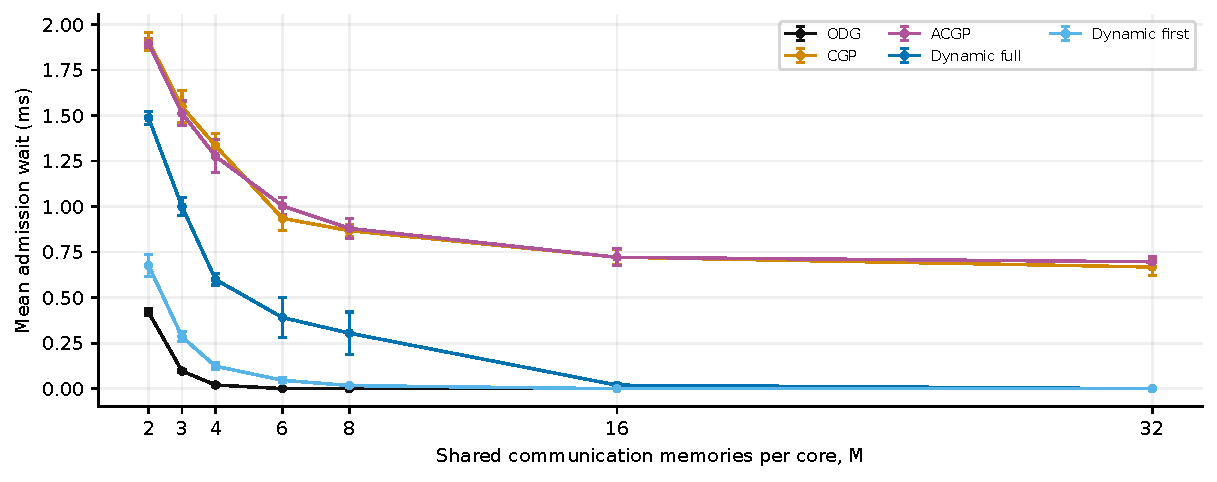
\includegraphics[width=.94\linewidth,height=.255\textheight,keepaspectratio]{figures/memory/mesh_shortest_reliable_average_admission_wait_ms.pdf}\captionof{figure}{Run-level mean and sample SD. Shared trace aliases are counted once.}\end{center}
\begin{center}{\scriptsize\setlength{\tabcolsep}{3pt}
\begin{tabular}{lrrrrr}
\toprule
M & ODG & CGP & ACGP & Dynamic full & Dynamic first \\
\midrule
2 & $0.4199\pm0.0197$ & $1.907\pm0.050$ & $1.896\pm0.024$ & $1.487\pm0.035$ & $0.6768\pm0.0582$ \\
3 & $0.0969\pm0.0073$ & $1.549\pm0.087$ & $1.513\pm0.067$ & $0.9992\pm0.0485$ & $0.2847\pm0.0275$ \\
4 & $0.0205\pm0.0007$ & $1.335\pm0.065$ & $1.277\pm0.090$ & $0.6000\pm0.0306$ & $0.1238\pm0.0192$ \\
6 & $0.0007\pm0.0006$ & $0.9356\pm0.0657$ & $1.004\pm0.047$ & $0.3909\pm0.1095$ & $0.0466\pm0.0122$ \\
8 & $0.0000\pm0.0001$ & $0.8681\pm0.0341$ & $0.8804\pm0.0532$ & $0.3053\pm0.1160$ & $0.0174\pm0.0073$ \\
16 & $0.0000\pm0.0000$ & $0.7223\pm0.0410$ & $0.7215\pm0.0467$ & $0.0196\pm0.0071$ & $0.0000\pm0.0000$ \\
32 & $0.0000\pm0.0000$ & $0.6681\pm0.0480$ & $0.6969\pm0.0310$ & $0.0000\pm0.0000$ & $0.0000\pm0.0000$ \\
\bottomrule\end{tabular}}
\captionof{table}{Mean $\pm$ sample SD; n/a denotes a metric outside that policy's instrumentation.}
{\footnotesize\href{https://github.com/sanjeevkrishnaa/Compiler-Driven-ACE/blob/codex/ace-scheduler-correctness/docs/latex/qft96_final/data/memory_mesh_shortest_reliable_average_admission_wait_ms.csv}{Exact CSV values and sample counts}}
\end{center}
\clearpage
\subsection*{Delivered EPR fidelity}
\begin{center}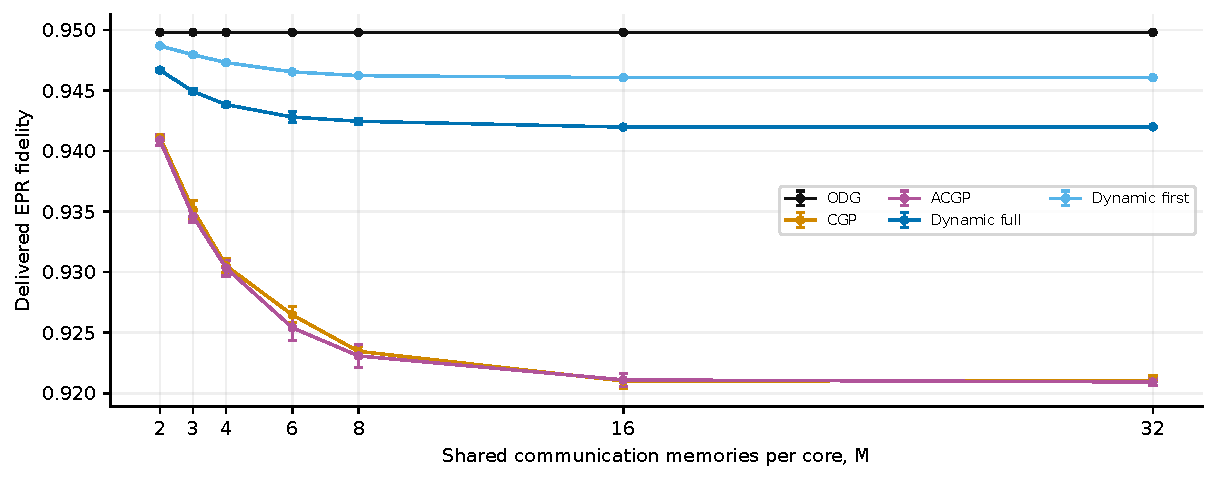
\includegraphics[width=.94\linewidth,height=.255\textheight,keepaspectratio]{figures/memory/mesh_shortest_reliable_average_delivered_epr_fidelity.pdf}\captionof{figure}{Run-level mean and sample SD. Shared trace aliases are counted once.}\end{center}
\begin{center}{\scriptsize\setlength{\tabcolsep}{3pt}
\begin{tabular}{lrrrrr}
\toprule
M & ODG & CGP & ACGP & Dynamic full & Dynamic first \\
\midrule
2 & $0.9498\pm0.0000$ & $0.9411\pm0.0002$ & $0.9409\pm0.0005$ & $0.9467\pm0.0001$ & $0.9487\pm0.0000$ \\
3 & $0.9498\pm0.0000$ & $0.9351\pm0.0008$ & $0.9346\pm0.0005$ & $0.9449\pm0.0002$ & $0.9480\pm0.0001$ \\
4 & $0.9498\pm0.0000$ & $0.9305\pm0.0006$ & $0.9303\pm0.0007$ & $0.9438\pm0.0001$ & $0.9473\pm0.0001$ \\
6 & $0.9498\pm0.0000$ & $0.9265\pm0.0007$ & $0.9254\pm0.0010$ & $0.9428\pm0.0004$ & $0.9465\pm0.0000$ \\
8 & $0.9498\pm0.0000$ & $0.9235\pm0.0004$ & $0.9231\pm0.0010$ & $0.9425\pm0.0002$ & $0.9462\pm0.0000$ \\
16 & $0.9498\pm0.0000$ & $0.9210\pm0.0006$ & $0.9211\pm0.0006$ & $0.9420\pm0.0000$ & $0.9461\pm0.0000$ \\
32 & $0.9498\pm0.0000$ & $0.9211\pm0.0004$ & $0.9209\pm0.0003$ & $0.9420\pm0.0000$ & $0.9461\pm0.0000$ \\
\bottomrule\end{tabular}}
\captionof{table}{Mean $\pm$ sample SD; n/a denotes a metric outside that policy's instrumentation.}
{\footnotesize\href{https://github.com/sanjeevkrishnaa/Compiler-Driven-ACE/blob/codex/ace-scheduler-correctness/docs/latex/qft96_final/data/memory_mesh_shortest_reliable_average_delivered_epr_fidelity.csv}{Exact CSV values and sample counts}}
\end{center}
\subsection*{Compiler readiness fraction}
\begin{center}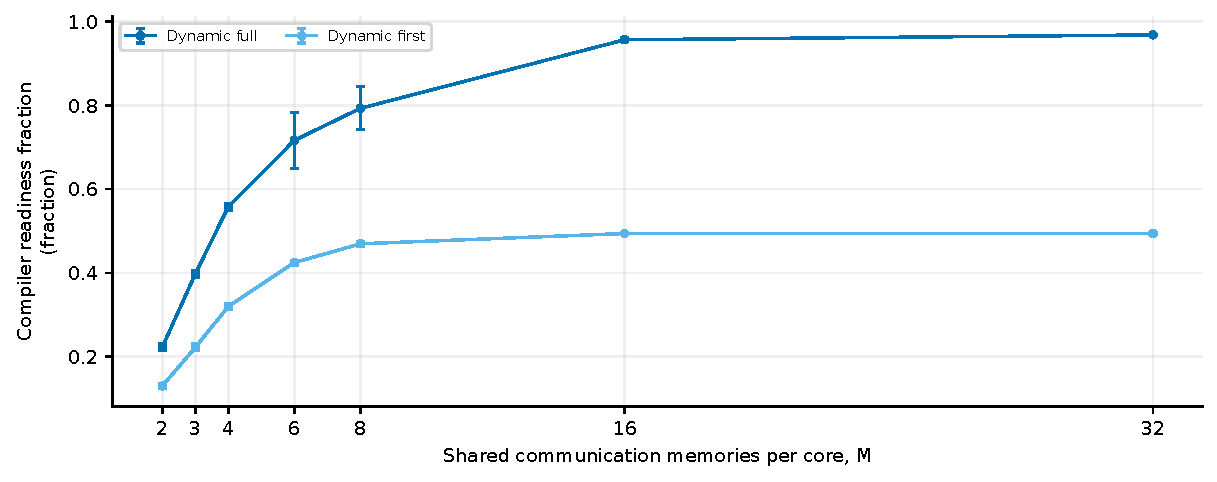
\includegraphics[width=.94\linewidth,height=.255\textheight,keepaspectratio]{figures/memory/mesh_shortest_reliable_pregenerated_success_rate.pdf}\captionof{figure}{Run-level mean and sample SD. Shared trace aliases are counted once.}\end{center}
\begin{center}{\scriptsize\setlength{\tabcolsep}{3pt}
\begin{tabular}{lrrrrr}
\toprule
M & ODG & CGP & ACGP & Dynamic full & Dynamic first \\
\midrule
2 & n/a & n/a & n/a & $0.2226\pm0.0087$ & $0.1299\pm0.0067$ \\
3 & n/a & n/a & n/a & $0.3976\pm0.0084$ & $0.2221\pm0.0083$ \\
4 & n/a & n/a & n/a & $0.5577\pm0.0084$ & $0.3197\pm0.0063$ \\
6 & n/a & n/a & n/a & $0.7165\pm0.0674$ & $0.4246\pm0.0058$ \\
8 & n/a & n/a & n/a & $0.7930\pm0.0516$ & $0.4695\pm0.0060$ \\
16 & n/a & n/a & n/a & $0.9567\pm0.0049$ & $0.4940\pm0.0016$ \\
32 & n/a & n/a & n/a & $0.9683\pm0.0013$ & $0.4940\pm0.0016$ \\
\bottomrule\end{tabular}}
\captionof{table}{Mean $\pm$ sample SD; n/a denotes a metric outside that policy's instrumentation.}
{\footnotesize\href{https://github.com/sanjeevkrishnaa/Compiler-Driven-ACE/blob/codex/ace-scheduler-correctness/docs/latex/qft96_final/data/memory_mesh_shortest_reliable_pregenerated_success_rate.csv}{Exact CSV values and sample counts}}
\end{center}
\clearpage
\subsection*{Intended compiler-hit fraction}
\begin{center}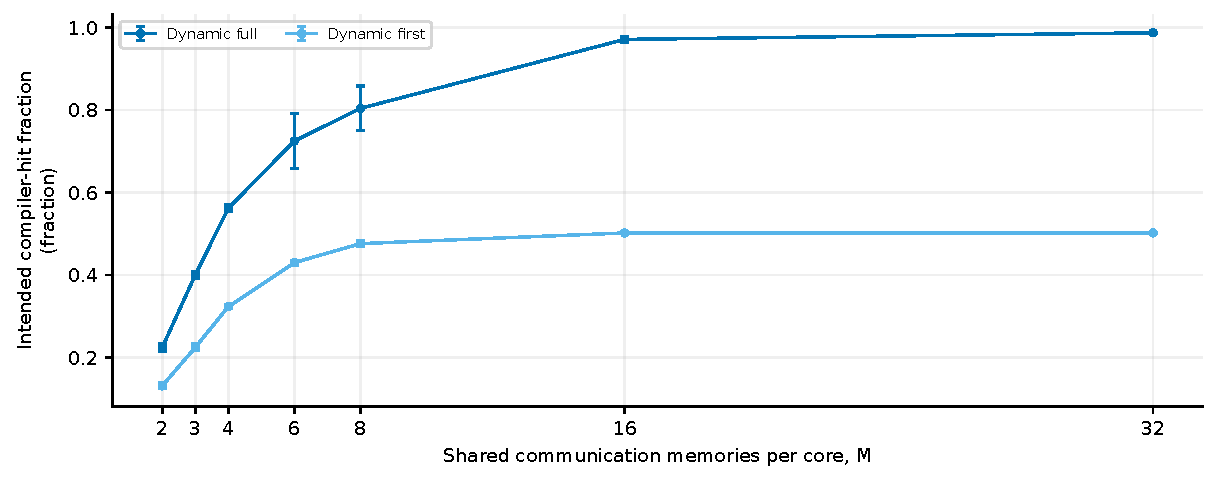
\includegraphics[width=.94\linewidth,height=.255\textheight,keepaspectratio]{figures/memory/mesh_shortest_reliable_intended_request_hit_rate.pdf}\captionof{figure}{Run-level mean and sample SD. Shared trace aliases are counted once.}\end{center}
\begin{center}{\scriptsize\setlength{\tabcolsep}{3pt}
\begin{tabular}{lrrrrr}
\toprule
M & ODG & CGP & ACGP & Dynamic full & Dynamic first \\
\midrule
2 & n/a & n/a & n/a & $0.2238\pm0.0089$ & $0.1309\pm0.0070$ \\
3 & n/a & n/a & n/a & $0.4000\pm0.0085$ & $0.2242\pm0.0085$ \\
4 & n/a & n/a & n/a & $0.5618\pm0.0079$ & $0.3231\pm0.0055$ \\
6 & n/a & n/a & n/a & $0.7248\pm0.0670$ & $0.4298\pm0.0063$ \\
8 & n/a & n/a & n/a & $0.8040\pm0.0543$ & $0.4759\pm0.0063$ \\
16 & n/a & n/a & n/a & $0.9713\pm0.0066$ & $0.5018\pm0.0015$ \\
32 & n/a & n/a & n/a & $0.9874\pm0.0011$ & $0.5018\pm0.0015$ \\
\bottomrule\end{tabular}}
\captionof{table}{Mean $\pm$ sample SD; n/a denotes a metric outside that policy's instrumentation.}
{\footnotesize\href{https://github.com/sanjeevkrishnaa/Compiler-Driven-ACE/blob/codex/ace-scheduler-correctness/docs/latex/qft96_final/data/memory_mesh_shortest_reliable_intended_request_hit_rate.csv}{Exact CSV values and sample counts}}
\end{center}
\subsection*{Compiler fallback fraction}
\begin{center}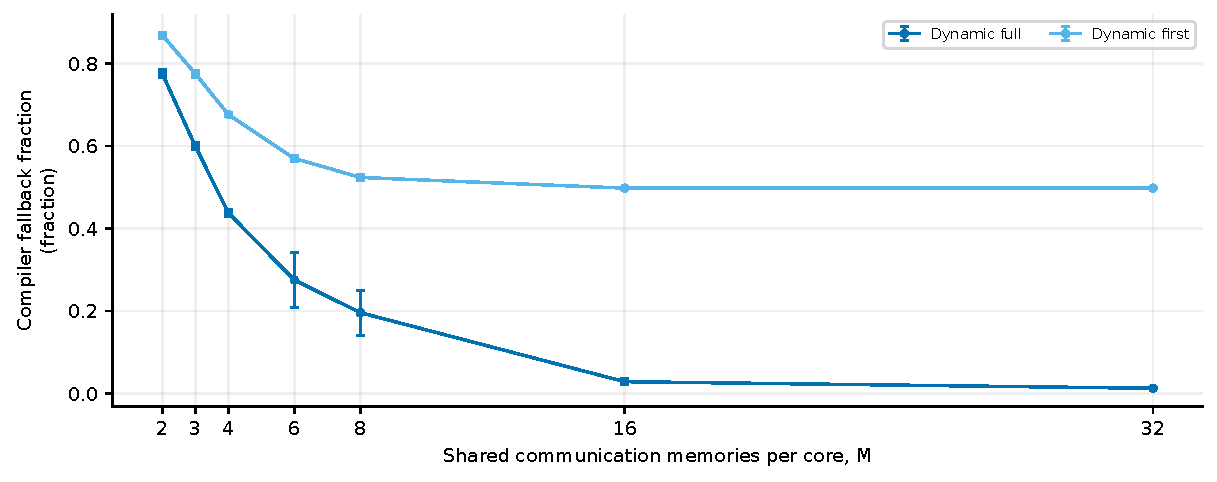
\includegraphics[width=.94\linewidth,height=.255\textheight,keepaspectratio]{figures/memory/mesh_shortest_reliable_on_demand_fallback_rate.pdf}\captionof{figure}{Run-level mean and sample SD. Shared trace aliases are counted once.}\end{center}
\begin{center}{\scriptsize\setlength{\tabcolsep}{3pt}
\begin{tabular}{lrrrrr}
\toprule
M & ODG & CGP & ACGP & Dynamic full & Dynamic first \\
\midrule
2 & n/a & n/a & n/a & $0.7762\pm0.0089$ & $0.8691\pm0.0070$ \\
3 & n/a & n/a & n/a & $0.6000\pm0.0085$ & $0.7758\pm0.0085$ \\
4 & n/a & n/a & n/a & $0.4382\pm0.0079$ & $0.6769\pm0.0055$ \\
6 & n/a & n/a & n/a & $0.2752\pm0.0670$ & $0.5702\pm0.0063$ \\
8 & n/a & n/a & n/a & $0.1960\pm0.0543$ & $0.5241\pm0.0063$ \\
16 & n/a & n/a & n/a & $0.0287\pm0.0066$ & $0.4982\pm0.0015$ \\
32 & n/a & n/a & n/a & $0.0126\pm0.0011$ & $0.4982\pm0.0015$ \\
\bottomrule\end{tabular}}
\captionof{table}{Mean $\pm$ sample SD; n/a denotes a metric outside that policy's instrumentation.}
{\footnotesize\href{https://github.com/sanjeevkrishnaa/Compiler-Driven-ACE/blob/codex/ace-scheduler-correctness/docs/latex/qft96_final/data/memory_mesh_shortest_reliable_on_demand_fallback_rate.csv}{Exact CSV values and sample counts}}
\end{center}
\clearpage
\subsection*{Compiler-cache waste}
\begin{center}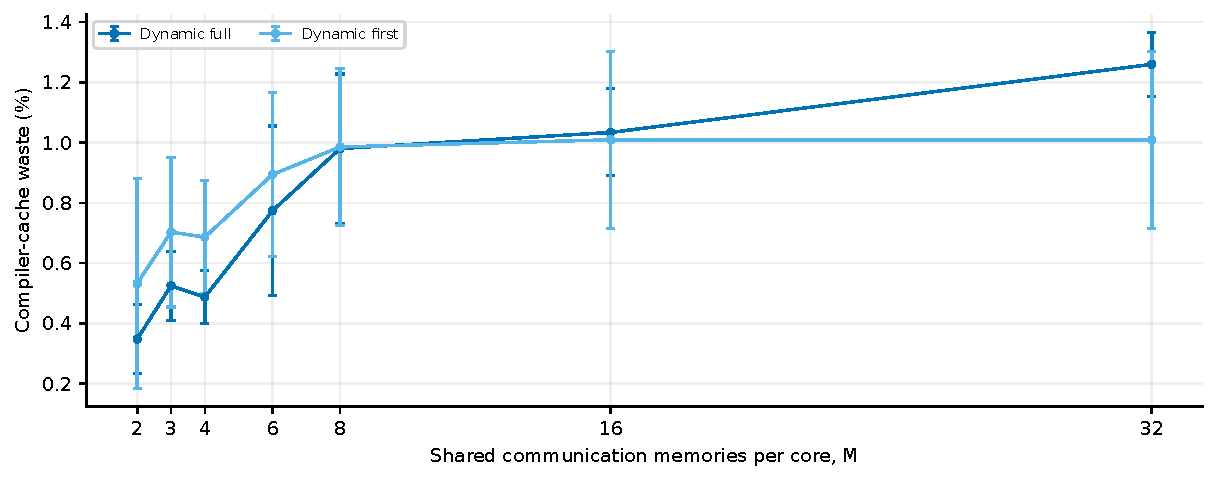
\includegraphics[width=.94\linewidth,height=.255\textheight,keepaspectratio]{figures/memory/mesh_shortest_reliable_compiler_waste_percentage.pdf}\captionof{figure}{Run-level mean and sample SD. Shared trace aliases are counted once.}\end{center}
\begin{center}{\scriptsize\setlength{\tabcolsep}{3pt}
\begin{tabular}{lrrrrr}
\toprule
M & ODG & CGP & ACGP & Dynamic full & Dynamic first \\
\midrule
2 & n/a & n/a & n/a & $0.3475\pm0.1140$ & $0.5320\pm0.3493$ \\
3 & n/a & n/a & n/a & $0.5248\pm0.1143$ & $0.7029\pm0.2488$ \\
4 & n/a & n/a & n/a & $0.4870\pm0.0873$ & $0.6862\pm0.1865$ \\
6 & n/a & n/a & n/a & $0.7735\pm0.2817$ & $0.8940\pm0.2733$ \\
8 & n/a & n/a & n/a & $0.9803\pm0.2475$ & $0.9856\pm0.2594$ \\
16 & n/a & n/a & n/a & $1.034\pm0.145$ & $1.009\pm0.294$ \\
32 & n/a & n/a & n/a & $1.260\pm0.106$ & $1.009\pm0.294$ \\
\bottomrule\end{tabular}}
\captionof{table}{Mean $\pm$ sample SD; n/a denotes a metric outside that policy's instrumentation.}
{\footnotesize\href{https://github.com/sanjeevkrishnaa/Compiler-Driven-ACE/blob/codex/ace-scheduler-correctness/docs/latex/qft96_final/data/memory_mesh_shortest_reliable_compiler_waste_percentage.csv}{Exact CSV values and sample counts}}
\end{center}
\subsection*{Native-protocol waste}
\begin{center}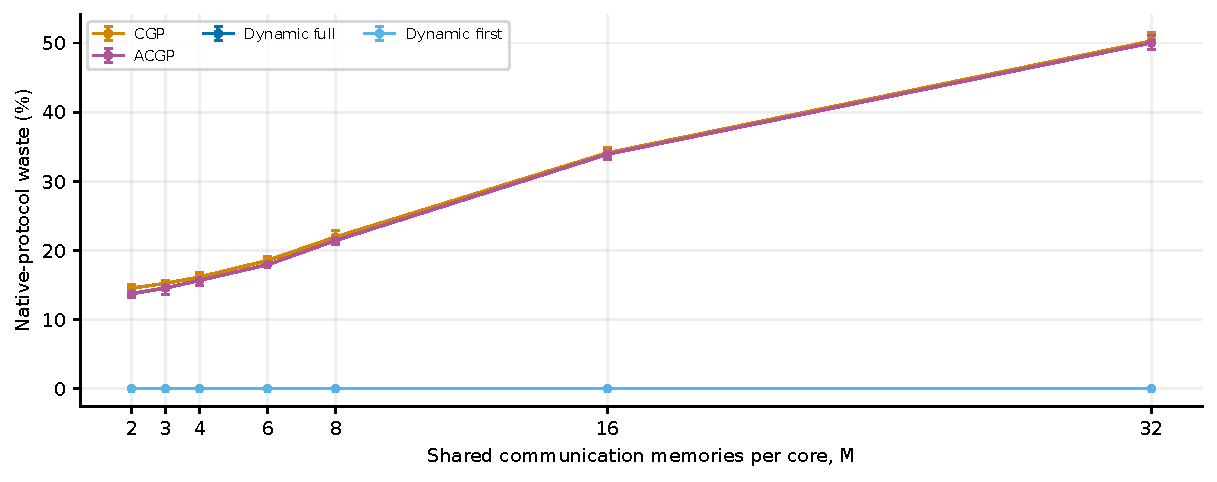
\includegraphics[width=.94\linewidth,height=.255\textheight,keepaspectratio]{figures/memory/mesh_shortest_reliable_protocol_waste_percentage.pdf}\captionof{figure}{Run-level mean and sample SD. Shared trace aliases are counted once.}\end{center}
\begin{center}{\scriptsize\setlength{\tabcolsep}{3pt}
\begin{tabular}{lrrrrr}
\toprule
M & ODG & CGP & ACGP & Dynamic full & Dynamic first \\
\midrule
2 & n/a & $14.553\pm0.495$ & $13.758\pm0.513$ & $0.0000\pm0.0000$ & $0.0000\pm0.0000$ \\
3 & n/a & $15.245\pm0.479$ & $14.578\pm0.972$ & $0.0000\pm0.0000$ & $0.0000\pm0.0000$ \\
4 & n/a & $16.160\pm0.590$ & $15.671\pm0.719$ & $0.0000\pm0.0000$ & $0.0000\pm0.0000$ \\
6 & n/a & $18.551\pm0.613$ & $17.943\pm0.129$ & $0.0000\pm0.0000$ & $0.0000\pm0.0000$ \\
8 & n/a & $21.953\pm0.935$ & $21.454\pm0.560$ & $0.0000\pm0.0000$ & $0.0000\pm0.0000$ \\
16 & n/a & $34.123\pm0.785$ & $33.927\pm0.719$ & $0.0000\pm0.0000$ & $0.0000\pm0.0000$ \\
32 & n/a & $50.300\pm1.267$ & $50.052\pm1.012$ & $0.0000\pm0.0000$ & $0.0000\pm0.0000$ \\
\bottomrule\end{tabular}}
\captionof{table}{Mean $\pm$ sample SD; n/a denotes a metric outside that policy's instrumentation.}
{\footnotesize\href{https://github.com/sanjeevkrishnaa/Compiler-Driven-ACE/blob/codex/ace-scheduler-correctness/docs/latex/qft96_final/data/memory_mesh_shortest_reliable_protocol_waste_percentage.csv}{Exact CSV values and sample counts}}
\end{center}
\clearpage
\subsection*{Compiler-pair expiry}
\begin{center}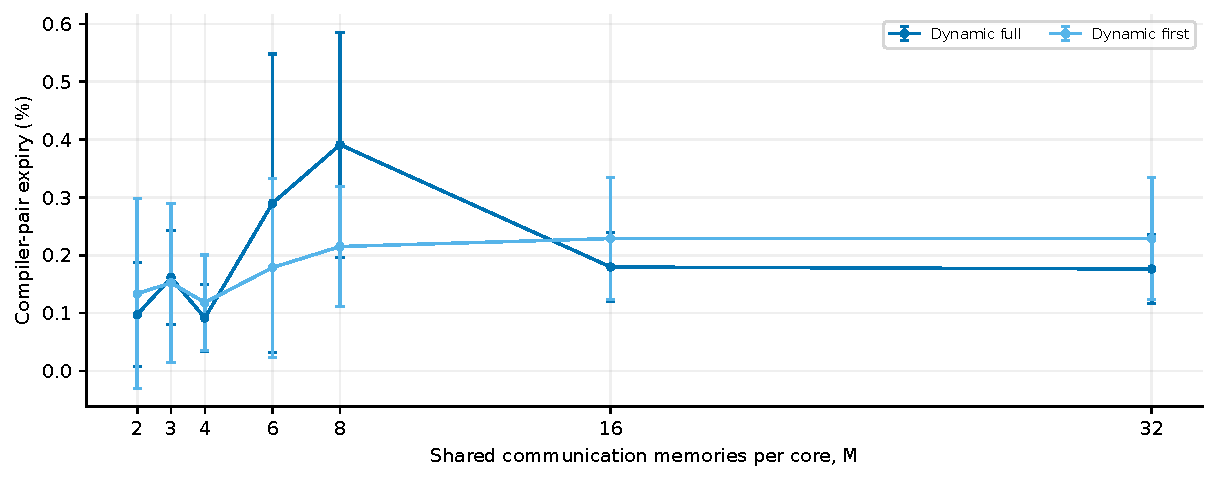
\includegraphics[width=.94\linewidth,height=.255\textheight,keepaspectratio]{figures/memory/mesh_shortest_reliable_compiler_expiry_percentage.pdf}\captionof{figure}{Run-level mean and sample SD. Shared trace aliases are counted once.}\end{center}
\begin{center}{\scriptsize\setlength{\tabcolsep}{3pt}
\begin{tabular}{lrrrrr}
\toprule
M & ODG & CGP & ACGP & Dynamic full & Dynamic first \\
\midrule
2 & n/a & n/a & n/a & $0.0973\pm0.0898$ & $0.1335\pm0.1642$ \\
3 & n/a & n/a & n/a & $0.1615\pm0.0810$ & $0.1526\pm0.1378$ \\
4 & n/a & n/a & n/a & $0.0916\pm0.0585$ & $0.1184\pm0.0822$ \\
6 & n/a & n/a & n/a & $0.2900\pm0.2580$ & $0.1788\pm0.1547$ \\
8 & n/a & n/a & n/a & $0.3913\pm0.1943$ & $0.2152\pm0.1031$ \\
16 & n/a & n/a & n/a & $0.1798\pm0.0591$ & $0.2290\pm0.1055$ \\
32 & n/a & n/a & n/a & $0.1763\pm0.0598$ & $0.2290\pm0.1055$ \\
\bottomrule\end{tabular}}
\captionof{table}{Mean $\pm$ sample SD; n/a denotes a metric outside that policy's instrumentation.}
{\footnotesize\href{https://github.com/sanjeevkrishnaa/Compiler-Driven-ACE/blob/codex/ace-scheduler-correctness/docs/latex/qft96_final/data/memory_mesh_shortest_reliable_compiler_expiry_percentage.csv}{Exact CSV values and sample counts}}
\end{center}
\subsection*{Used compiler-pair storage time}
\begin{center}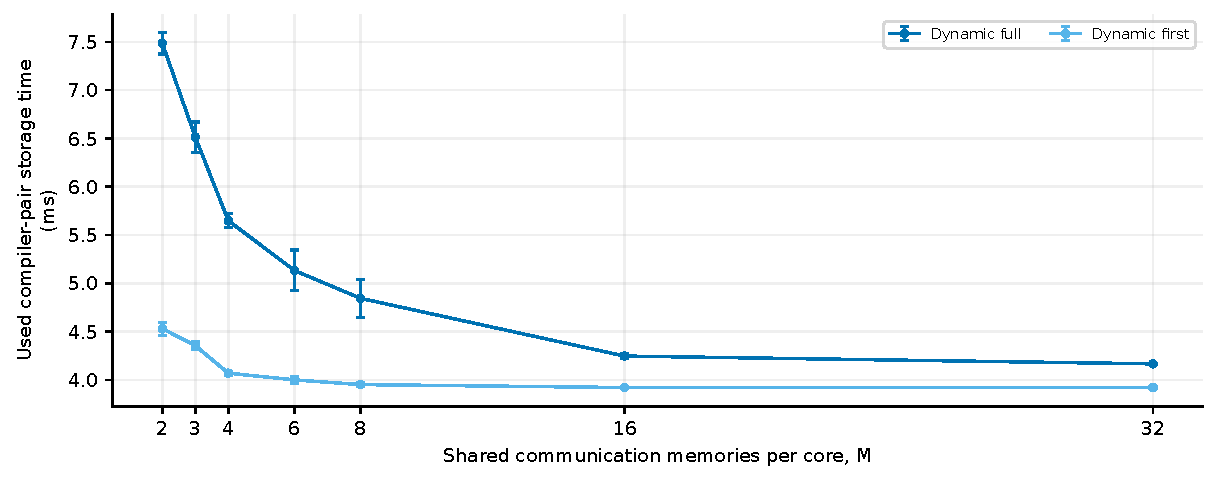
\includegraphics[width=.94\linewidth,height=.255\textheight,keepaspectratio]{figures/memory/mesh_shortest_reliable_average_storage_time_ms.pdf}\captionof{figure}{Run-level mean and sample SD. Shared trace aliases are counted once.}\end{center}
\begin{center}{\scriptsize\setlength{\tabcolsep}{3pt}
\begin{tabular}{lrrrrr}
\toprule
M & ODG & CGP & ACGP & Dynamic full & Dynamic first \\
\midrule
2 & n/a & n/a & n/a & $7.486\pm0.112$ & $4.531\pm0.068$ \\
3 & n/a & n/a & n/a & $6.514\pm0.156$ & $4.355\pm0.041$ \\
4 & n/a & n/a & n/a & $5.649\pm0.071$ & $4.070\pm0.019$ \\
6 & n/a & n/a & n/a & $5.133\pm0.211$ & $4.001\pm0.037$ \\
8 & n/a & n/a & n/a & $4.845\pm0.196$ & $3.952\pm0.019$ \\
16 & n/a & n/a & n/a & $4.247\pm0.027$ & $3.921\pm0.012$ \\
32 & n/a & n/a & n/a & $4.166\pm0.005$ & $3.921\pm0.012$ \\
\bottomrule\end{tabular}}
\captionof{table}{Mean $\pm$ sample SD; n/a denotes a metric outside that policy's instrumentation.}
{\footnotesize\href{https://github.com/sanjeevkrishnaa/Compiler-Driven-ACE/blob/codex/ace-scheduler-correctness/docs/latex/qft96_final/data/memory_mesh_shortest_reliable_average_storage_time_ms.csv}{Exact CSV values and sample counts}}
\end{center}
\clearpage
\subsection*{Delivered-hop throughput}
\begin{center}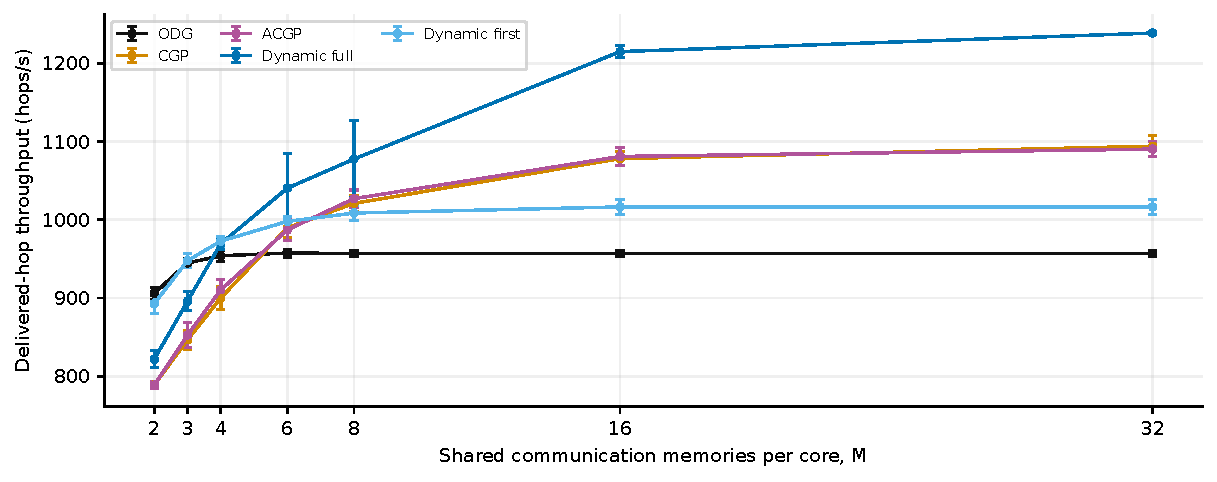
\includegraphics[width=.94\linewidth,height=.255\textheight,keepaspectratio]{figures/memory/mesh_shortest_reliable_hop_throughput_s.pdf}\captionof{figure}{Run-level mean and sample SD. Shared trace aliases are counted once.}\end{center}
\begin{center}{\scriptsize\setlength{\tabcolsep}{3pt}
\begin{tabular}{lrrrrr}
\toprule
M & ODG & CGP & ACGP & Dynamic full & Dynamic first \\
\midrule
2 & $905.76\pm8.15$ & $788.85\pm4.92$ & $788.75\pm3.98$ & $821.61\pm10.93$ & $892.79\pm13.16$ \\
3 & $944.69\pm5.99$ & $846.52\pm11.93$ & $852.55\pm15.77$ & $895.90\pm12.18$ & $947.66\pm8.99$ \\
4 & $953.88\pm6.91$ & $900.10\pm14.72$ & $910.38\pm12.82$ & $969.43\pm7.48$ & $972.64\pm6.28$ \\
6 & $957.40\pm5.06$ & $989.64\pm13.04$ & $987.06\pm13.48$ & $1040.35\pm44.31$ & $997.83\pm6.04$ \\
8 & $956.81\pm3.94$ & $1020.92\pm10.52$ & $1026.88\pm11.06$ & $1077.45\pm49.03$ & $1008.54\pm9.10$ \\
16 & $956.81\pm3.96$ & $1078.06\pm9.00$ & $1080.84\pm11.84$ & $1214.84\pm7.44$ & $1016.34\pm9.40$ \\
32 & $956.81\pm3.96$ & $1093.98\pm13.19$ & $1090.23\pm9.98$ & $1238.57\pm0.93$ & $1016.34\pm9.40$ \\
\bottomrule\end{tabular}}
\captionof{table}{Mean $\pm$ sample SD; n/a denotes a metric outside that policy's instrumentation.}
{\footnotesize\href{https://github.com/sanjeevkrishnaa/Compiler-Driven-ACE/blob/codex/ace-scheduler-correctness/docs/latex/qft96_final/data/memory_mesh_shortest_reliable_hop_throughput_s.csv}{Exact CSV values and sample counts}}
\end{center}
\subsection*{Completion fraction}
\begin{center}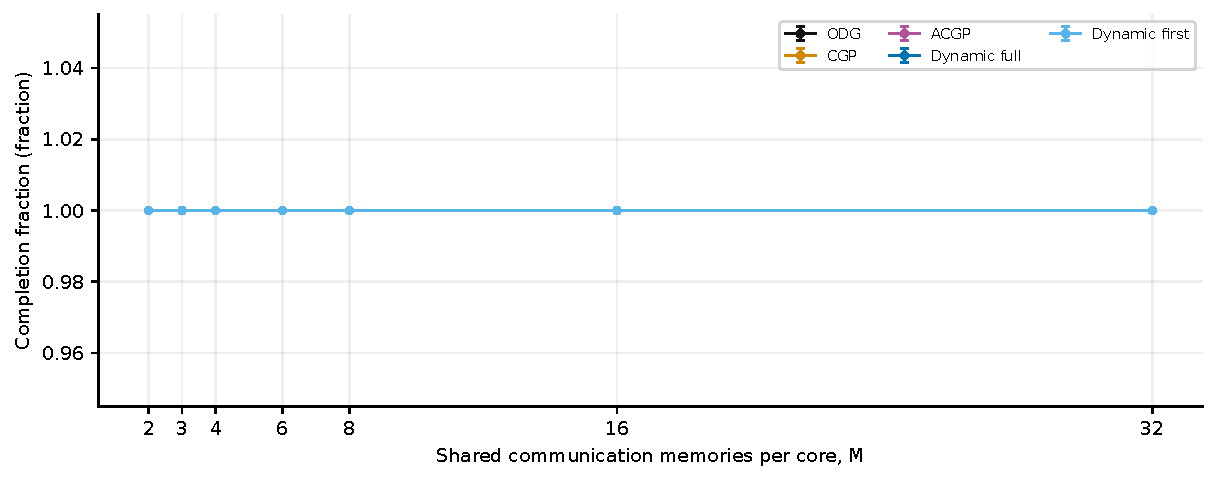
\includegraphics[width=.94\linewidth,height=.255\textheight,keepaspectratio]{figures/memory/mesh_shortest_reliable_completion_rate.pdf}\captionof{figure}{Run-level mean and sample SD. Shared trace aliases are counted once.}\end{center}
\begin{center}{\scriptsize\setlength{\tabcolsep}{3pt}
\begin{tabular}{lrrrrr}
\toprule
M & ODG & CGP & ACGP & Dynamic full & Dynamic first \\
\midrule
2 & $1.000\pm0.000$ & $1.000\pm0.000$ & $1.000\pm0.000$ & $1.000\pm0.000$ & $1.000\pm0.000$ \\
3 & $1.000\pm0.000$ & $1.000\pm0.000$ & $1.000\pm0.000$ & $1.000\pm0.000$ & $1.000\pm0.000$ \\
4 & $1.000\pm0.000$ & $1.000\pm0.000$ & $1.000\pm0.000$ & $1.000\pm0.000$ & $1.000\pm0.000$ \\
6 & $1.000\pm0.000$ & $1.000\pm0.000$ & $1.000\pm0.000$ & $1.000\pm0.000$ & $1.000\pm0.000$ \\
8 & $1.000\pm0.000$ & $1.000\pm0.000$ & $1.000\pm0.000$ & $1.000\pm0.000$ & $1.000\pm0.000$ \\
16 & $1.000\pm0.000$ & $1.000\pm0.000$ & $1.000\pm0.000$ & $1.000\pm0.000$ & $1.000\pm0.000$ \\
32 & $1.000\pm0.000$ & $1.000\pm0.000$ & $1.000\pm0.000$ & $1.000\pm0.000$ & $1.000\pm0.000$ \\
\bottomrule\end{tabular}}
\captionof{table}{Mean $\pm$ sample SD; n/a denotes a metric outside that policy's instrumentation.}
{\footnotesize\href{https://github.com/sanjeevkrishnaa/Compiler-Driven-ACE/blob/codex/ace-scheduler-correctness/docs/latex/qft96_final/data/memory_mesh_shortest_reliable_completion_rate.csv}{Exact CSV values and sample counts}}
\end{center}
\clearpage
\subsection*{Maximum admission wait}
\begin{center}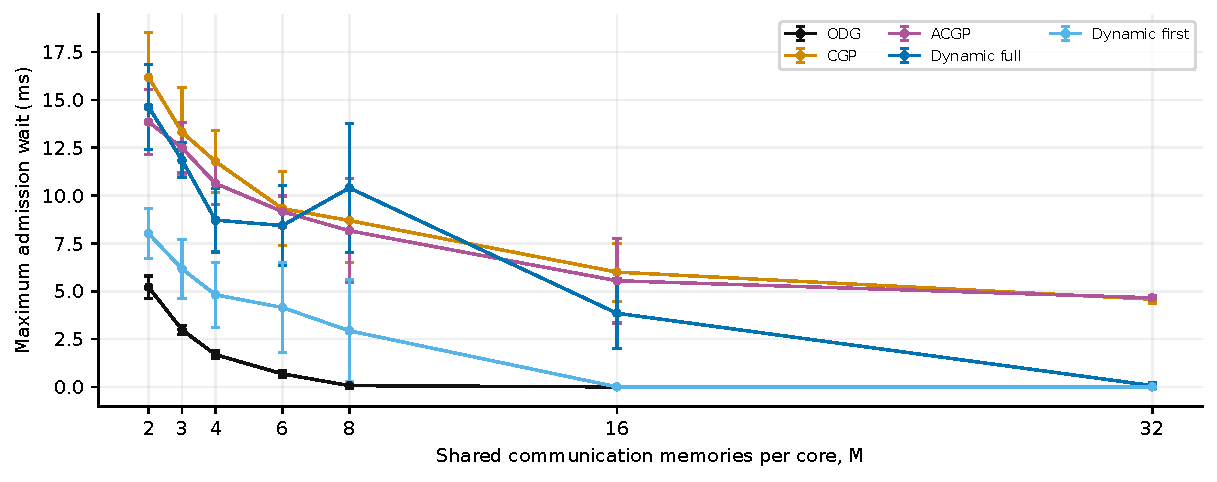
\includegraphics[width=.94\linewidth,height=.255\textheight,keepaspectratio]{figures/memory/mesh_shortest_reliable_max_admission_wait_ms.pdf}\captionof{figure}{Run-level mean and sample SD. Shared trace aliases are counted once.}\end{center}
\begin{center}{\scriptsize\setlength{\tabcolsep}{3pt}
\begin{tabular}{lrrrrr}
\toprule
M & ODG & CGP & ACGP & Dynamic full & Dynamic first \\
\midrule
2 & $5.217\pm0.581$ & $16.183\pm2.352$ & $13.850\pm1.714$ & $14.634\pm2.210$ & $8.017\pm1.286$ \\
3 & $2.983\pm0.248$ & $13.317\pm2.337$ & $12.494\pm1.313$ & $11.850\pm0.916$ & $6.167\pm1.546$ \\
4 & $1.683\pm0.194$ & $11.784\pm1.614$ & $10.634\pm1.117$ & $8.717\pm1.664$ & $4.817\pm1.708$ \\
6 & $0.6834\pm0.1941$ & $9.317\pm1.920$ & $9.167\pm0.812$ & $8.434\pm2.085$ & $4.150\pm2.374$ \\
8 & $0.0667\pm0.1633$ & $8.697\pm2.182$ & $8.163\pm2.716$ & $10.400\pm3.368$ & $2.933\pm2.666$ \\
16 & $0.0000\pm0.0000$ & $6.000\pm1.513$ & $5.550\pm2.210$ & $3.850\pm1.838$ & $0.0000\pm0.0000$ \\
32 & $0.0000\pm0.0000$ & $4.583\pm0.214$ & $4.657\pm0.136$ & $0.0667\pm0.1633$ & $0.0000\pm0.0000$ \\
\bottomrule\end{tabular}}
\captionof{table}{Mean $\pm$ sample SD; n/a denotes a metric outside that policy's instrumentation.}
{\footnotesize\href{https://github.com/sanjeevkrishnaa/Compiler-Driven-ACE/blob/codex/ace-scheduler-correctness/docs/latex/qft96_final/data/memory_mesh_shortest_reliable_max_admission_wait_ms.csv}{Exact CSV values and sample counts}}
\end{center}
\subsection*{Requests with admission wait}
\begin{center}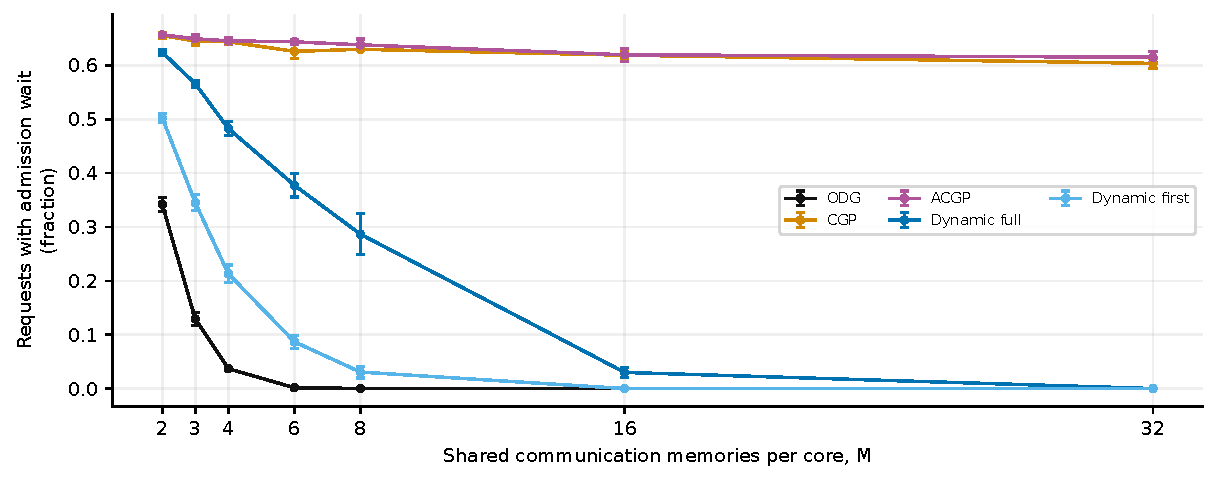
\includegraphics[width=.94\linewidth,height=.255\textheight,keepaspectratio]{figures/memory/mesh_shortest_reliable_requests_that_waited_fraction.pdf}\captionof{figure}{Run-level mean and sample SD. Shared trace aliases are counted once.}\end{center}
\begin{center}{\scriptsize\setlength{\tabcolsep}{3pt}
\begin{tabular}{lrrrrr}
\toprule
M & ODG & CGP & ACGP & Dynamic full & Dynamic first \\
\midrule
2 & $0.3419\pm0.0136$ & $0.6555\pm0.0058$ & $0.6567\pm0.0030$ & $0.6242\pm0.0053$ & $0.5027\pm0.0083$ \\
3 & $0.1292\pm0.0118$ & $0.6452\pm0.0077$ & $0.6494\pm0.0074$ & $0.5659\pm0.0065$ & $0.3449\pm0.0149$ \\
4 & $0.0369\pm0.0026$ & $0.6439\pm0.0058$ & $0.6455\pm0.0068$ & $0.4828\pm0.0126$ & $0.2133\pm0.0162$ \\
6 & $0.0016\pm0.0013$ & $0.6260\pm0.0128$ & $0.6437\pm0.0048$ & $0.3775\pm0.0218$ & $0.0869\pm0.0123$ \\
8 & $0.0002\pm0.0005$ & $0.6299\pm0.0024$ & $0.6381\pm0.0108$ & $0.2866\pm0.0384$ & $0.0307\pm0.0110$ \\
16 & $0.0000\pm0.0000$ & $0.6189\pm0.0065$ & $0.6196\pm0.0123$ & $0.0300\pm0.0090$ & $0.0000\pm0.0000$ \\
32 & $0.0000\pm0.0000$ & $0.6037\pm0.0091$ & $0.6151\pm0.0101$ & $0.0000\pm0.0001$ & $0.0000\pm0.0000$ \\
\bottomrule\end{tabular}}
\captionof{table}{Mean $\pm$ sample SD; n/a denotes a metric outside that policy's instrumentation.}
{\footnotesize\href{https://github.com/sanjeevkrishnaa/Compiler-Driven-ACE/blob/codex/ace-scheduler-correctness/docs/latex/qft96_final/data/memory_mesh_shortest_reliable_requests_that_waited_fraction.csv}{Exact CSV values and sample counts}}
\end{center}
\clearpage
\subsection*{Recorded reservation-setup counter}
\begin{center}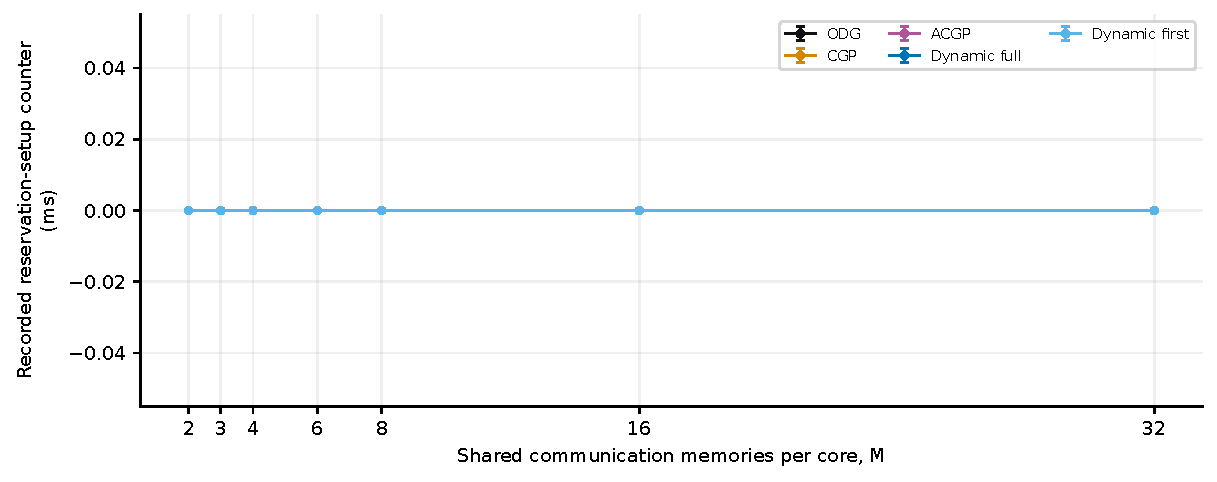
\includegraphics[width=.94\linewidth,height=.255\textheight,keepaspectratio]{figures/memory/mesh_shortest_reliable_avg_reservation_setup_time_ms.pdf}\captionof{figure}{Run-level mean and sample SD. Shared trace aliases are counted once.}\end{center}
\begin{center}{\scriptsize\setlength{\tabcolsep}{3pt}
\begin{tabular}{lrrrrr}
\toprule
M & ODG & CGP & ACGP & Dynamic full & Dynamic first \\
\midrule
2 & $0.0000\pm0.0000$ & $0.0000\pm0.0000$ & $0.0000\pm0.0000$ & $0.0000\pm0.0000$ & $0.0000\pm0.0000$ \\
3 & $0.0000\pm0.0000$ & $0.0000\pm0.0000$ & $0.0000\pm0.0000$ & $0.0000\pm0.0000$ & $0.0000\pm0.0000$ \\
4 & $0.0000\pm0.0000$ & $0.0000\pm0.0000$ & $0.0000\pm0.0000$ & $0.0000\pm0.0000$ & $0.0000\pm0.0000$ \\
6 & $0.0000\pm0.0000$ & $0.0000\pm0.0000$ & $0.0000\pm0.0000$ & $0.0000\pm0.0000$ & $0.0000\pm0.0000$ \\
8 & $0.0000\pm0.0000$ & $0.0000\pm0.0000$ & $0.0000\pm0.0000$ & $0.0000\pm0.0000$ & $0.0000\pm0.0000$ \\
16 & $0.0000\pm0.0000$ & $0.0000\pm0.0000$ & $0.0000\pm0.0000$ & $0.0000\pm0.0000$ & $0.0000\pm0.0000$ \\
32 & $0.0000\pm0.0000$ & $0.0000\pm0.0000$ & $0.0000\pm0.0000$ & $0.0000\pm0.0000$ & $0.0000\pm0.0000$ \\
\bottomrule\end{tabular}}
\captionof{table}{Mean $\pm$ sample SD; n/a denotes a metric outside that policy's instrumentation.}
{\footnotesize\href{https://github.com/sanjeevkrishnaa/Compiler-Driven-ACE/blob/codex/ace-scheduler-correctness/docs/latex/qft96_final/data/memory_mesh_shortest_reliable_avg_reservation_setup_time_ms.csv}{Exact CSV values and sample counts}}
\end{center}
\subsection*{Mean generation/service time}
\begin{center}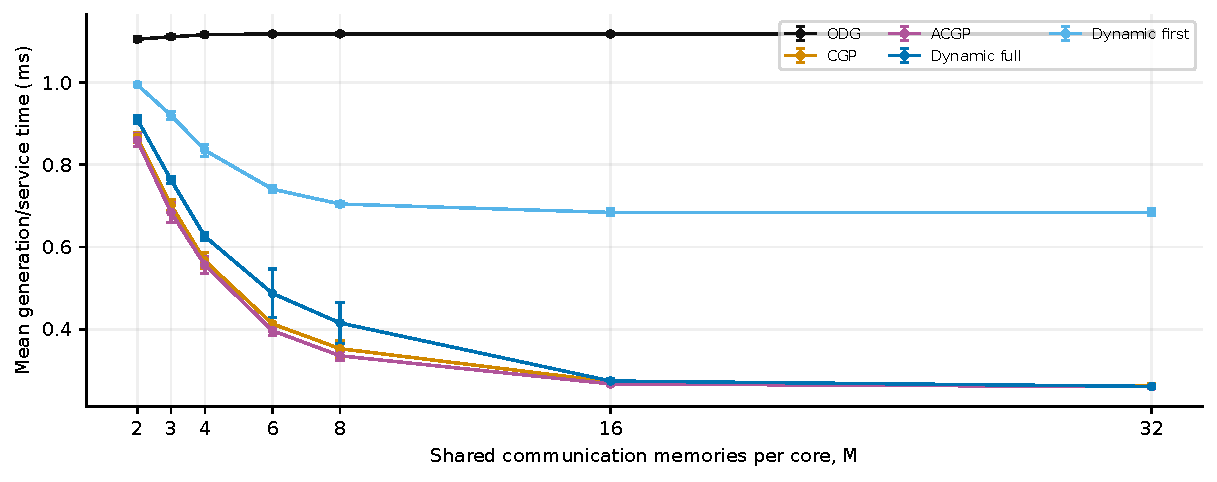
\includegraphics[width=.94\linewidth,height=.255\textheight,keepaspectratio]{figures/memory/mesh_shortest_reliable_avg_entanglement_generation_time_ms.pdf}\captionof{figure}{Run-level mean and sample SD. Shared trace aliases are counted once.}\end{center}
\begin{center}{\scriptsize\setlength{\tabcolsep}{3pt}
\begin{tabular}{lrrrrr}
\toprule
M & ODG & CGP & ACGP & Dynamic full & Dynamic first \\
\midrule
2 & $1.106\pm0.006$ & $0.8669\pm0.0124$ & $0.8600\pm0.0153$ & $0.9110\pm0.0092$ & $0.9952\pm0.0056$ \\
3 & $1.112\pm0.005$ & $0.7018\pm0.0143$ & $0.6844\pm0.0242$ & $0.7633\pm0.0080$ & $0.9207\pm0.0095$ \\
4 & $1.117\pm0.004$ & $0.5666\pm0.0197$ & $0.5561\pm0.0205$ & $0.6258\pm0.0107$ & $0.8356\pm0.0149$ \\
6 & $1.119\pm0.004$ & $0.4128\pm0.0148$ & $0.3965\pm0.0112$ & $0.4870\pm0.0595$ & $0.7408\pm0.0083$ \\
8 & $1.118\pm0.004$ & $0.3526\pm0.0210$ & $0.3352\pm0.0109$ & $0.4151\pm0.0497$ & $0.7046\pm0.0054$ \\
16 & $1.118\pm0.004$ & $0.2719\pm0.0053$ & $0.2668\pm0.0039$ & $0.2739\pm0.0061$ & $0.6841\pm0.0083$ \\
32 & $1.118\pm0.004$ & $0.2611\pm0.0061$ & $0.2599\pm0.0031$ & $0.2607\pm0.0011$ & $0.6841\pm0.0083$ \\
\bottomrule\end{tabular}}
\captionof{table}{Mean $\pm$ sample SD; n/a denotes a metric outside that policy's instrumentation.}
{\footnotesize\href{https://github.com/sanjeevkrishnaa/Compiler-Driven-ACE/blob/codex/ace-scheduler-correctness/docs/latex/qft96_final/data/memory_mesh_shortest_reliable_avg_entanglement_generation_time_ms.csv}{Exact CSV values and sample counts}}
\end{center}
\clearpage
\subsection*{Recorded retry-wait time}
\begin{center}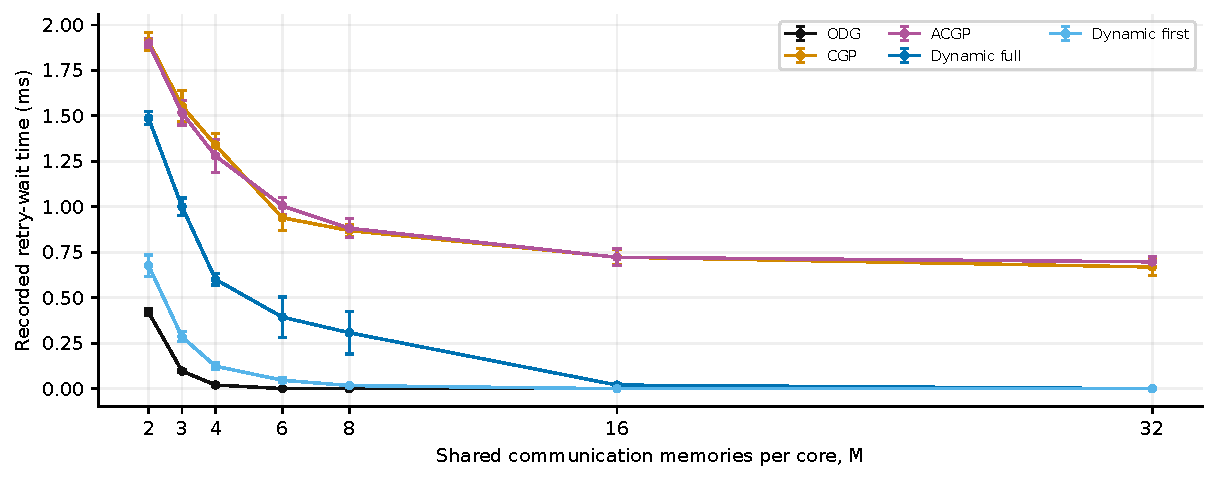
\includegraphics[width=.94\linewidth,height=.255\textheight,keepaspectratio]{figures/memory/mesh_shortest_reliable_avg_retry_wait_time_ms.pdf}\captionof{figure}{Run-level mean and sample SD. Shared trace aliases are counted once.}\end{center}
\begin{center}{\scriptsize\setlength{\tabcolsep}{3pt}
\begin{tabular}{lrrrrr}
\toprule
M & ODG & CGP & ACGP & Dynamic full & Dynamic first \\
\midrule
2 & $0.4199\pm0.0197$ & $1.909\pm0.050$ & $1.899\pm0.024$ & $1.487\pm0.035$ & $0.6768\pm0.0582$ \\
3 & $0.0969\pm0.0073$ & $1.553\pm0.084$ & $1.516\pm0.067$ & $0.9999\pm0.0484$ & $0.2848\pm0.0274$ \\
4 & $0.0205\pm0.0007$ & $1.339\pm0.063$ & $1.279\pm0.091$ & $0.6014\pm0.0313$ & $0.1240\pm0.0192$ \\
6 & $0.0007\pm0.0006$ & $0.9397\pm0.0707$ & $1.005\pm0.047$ & $0.3935\pm0.1107$ & $0.0467\pm0.0122$ \\
8 & $0.0000\pm0.0001$ & $0.8696\pm0.0338$ & $0.8822\pm0.0531$ & $0.3079\pm0.1170$ & $0.0174\pm0.0074$ \\
16 & $0.0000\pm0.0000$ & $0.7232\pm0.0409$ & $0.7222\pm0.0465$ & $0.0202\pm0.0073$ & $0.0000\pm0.0000$ \\
32 & $0.0000\pm0.0000$ & $0.6689\pm0.0479$ & $0.6974\pm0.0310$ & $0.0000\pm0.0000$ & $0.0000\pm0.0000$ \\
\bottomrule\end{tabular}}
\captionof{table}{Mean $\pm$ sample SD; n/a denotes a metric outside that policy's instrumentation.}
{\footnotesize\href{https://github.com/sanjeevkrishnaa/Compiler-Driven-ACE/blob/codex/ace-scheduler-correctness/docs/latex/qft96_final/data/memory_mesh_shortest_reliable_avg_retry_wait_time_ms.csv}{Exact CSV values and sample counts}}
\end{center}
\subsection*{Request retries}
\begin{center}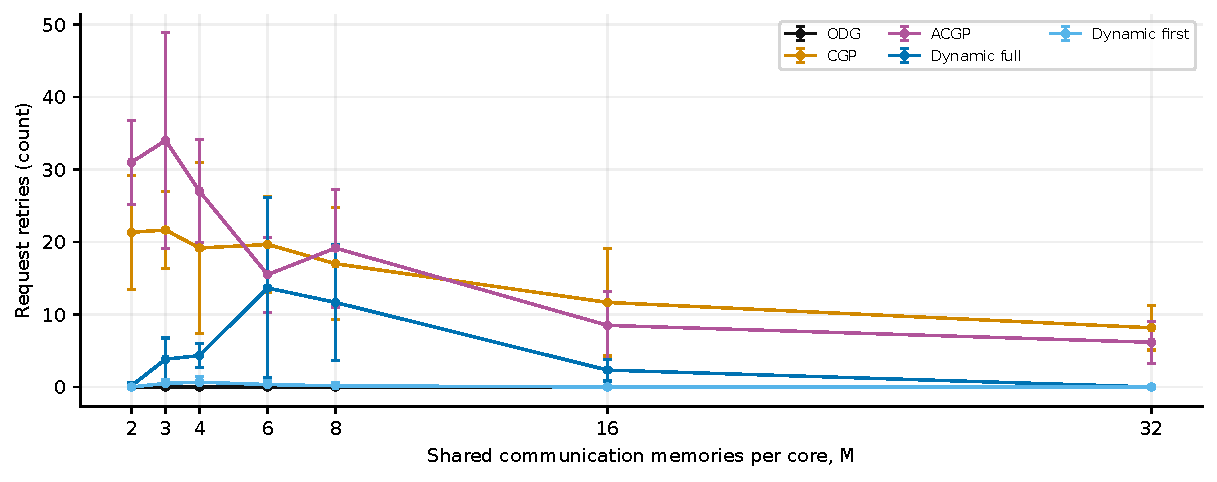
\includegraphics[width=.94\linewidth,height=.255\textheight,keepaspectratio]{figures/memory/mesh_shortest_reliable_total_retries.pdf}\captionof{figure}{Run-level mean and sample SD. Shared trace aliases are counted once.}\end{center}
\begin{center}{\scriptsize\setlength{\tabcolsep}{3pt}
\begin{tabular}{lrrrrr}
\toprule
M & ODG & CGP & ACGP & Dynamic full & Dynamic first \\
\midrule
2 & $0.0000\pm0.0000$ & $21.333\pm7.891$ & $31.000\pm5.762$ & $0.1667\pm0.4082$ & $0.0000\pm0.0000$ \\
3 & $0.0000\pm0.0000$ & $21.667\pm5.354$ & $34.000\pm14.926$ & $3.833\pm2.927$ & $0.5000\pm0.5477$ \\
4 & $0.0000\pm0.0000$ & $19.167\pm11.822$ & $27.000\pm7.099$ & $4.333\pm1.633$ & $0.6667\pm0.8165$ \\
6 & $0.0000\pm0.0000$ & $19.667\pm6.653$ & $15.500\pm5.167$ & $13.667\pm12.420$ & $0.3333\pm0.5164$ \\
8 & $0.0000\pm0.0000$ & $17.000\pm7.720$ & $19.167\pm8.134$ & $11.667\pm8.042$ & $0.1667\pm0.4082$ \\
16 & $0.0000\pm0.0000$ & $11.667\pm7.394$ & $8.500\pm4.722$ & $2.333\pm1.506$ & $0.0000\pm0.0000$ \\
32 & $0.0000\pm0.0000$ & $8.167\pm3.061$ & $6.167\pm2.927$ & $0.0000\pm0.0000$ & $0.0000\pm0.0000$ \\
\bottomrule\end{tabular}}
\captionof{table}{Mean $\pm$ sample SD; n/a denotes a metric outside that policy's instrumentation.}
{\footnotesize\href{https://github.com/sanjeevkrishnaa/Compiler-Driven-ACE/blob/codex/ace-scheduler-correctness/docs/latex/qft96_final/data/memory_mesh_shortest_reliable_total_retries.csv}{Exact CSV values and sample counts}}
\end{center}
\clearpage
\subsection*{Requests with retries}
\begin{center}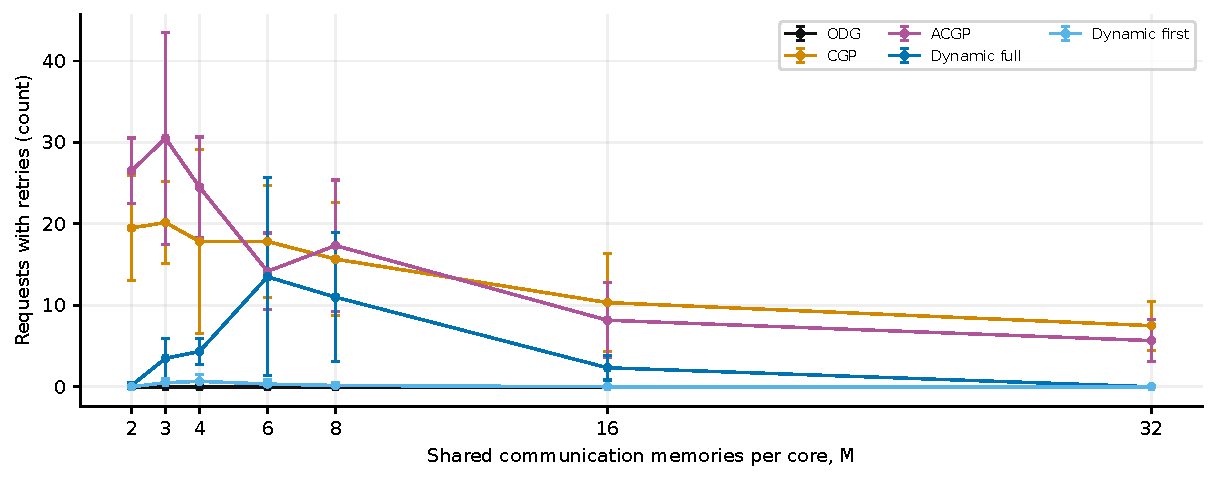
\includegraphics[width=.94\linewidth,height=.255\textheight,keepaspectratio]{figures/memory/mesh_shortest_reliable_requests_with_retries.pdf}\captionof{figure}{Run-level mean and sample SD. Shared trace aliases are counted once.}\end{center}
\begin{center}{\scriptsize\setlength{\tabcolsep}{3pt}
\begin{tabular}{lrrrrr}
\toprule
M & ODG & CGP & ACGP & Dynamic full & Dynamic first \\
\midrule
2 & $0.0000\pm0.0000$ & $19.500\pm6.442$ & $26.500\pm4.037$ & $0.1667\pm0.4082$ & $0.0000\pm0.0000$ \\
3 & $0.0000\pm0.0000$ & $20.167\pm5.037$ & $30.500\pm13.004$ & $3.500\pm2.429$ & $0.5000\pm0.5477$ \\
4 & $0.0000\pm0.0000$ & $17.833\pm11.286$ & $24.500\pm6.156$ & $4.333\pm1.633$ & $0.6667\pm0.8165$ \\
6 & $0.0000\pm0.0000$ & $17.833\pm6.824$ & $14.167\pm4.708$ & $13.500\pm12.161$ & $0.3333\pm0.5164$ \\
8 & $0.0000\pm0.0000$ & $15.667\pm6.919$ & $17.333\pm8.042$ & $11.000\pm7.899$ & $0.1667\pm0.4082$ \\
16 & $0.0000\pm0.0000$ & $10.333\pm6.055$ & $8.167\pm4.622$ & $2.333\pm1.506$ & $0.0000\pm0.0000$ \\
32 & $0.0000\pm0.0000$ & $7.500\pm3.017$ & $5.667\pm2.582$ & $0.0000\pm0.0000$ & $0.0000\pm0.0000$ \\
\bottomrule\end{tabular}}
\captionof{table}{Mean $\pm$ sample SD; n/a denotes a metric outside that policy's instrumentation.}
{\footnotesize\href{https://github.com/sanjeevkrishnaa/Compiler-Driven-ACE/blob/codex/ace-scheduler-correctness/docs/latex/qft96_final/data/memory_mesh_shortest_reliable_requests_with_retries.csv}{Exact CSV values and sample counts}}
\end{center}
\subsection*{Native-protocol generated-pair counter}
\begin{center}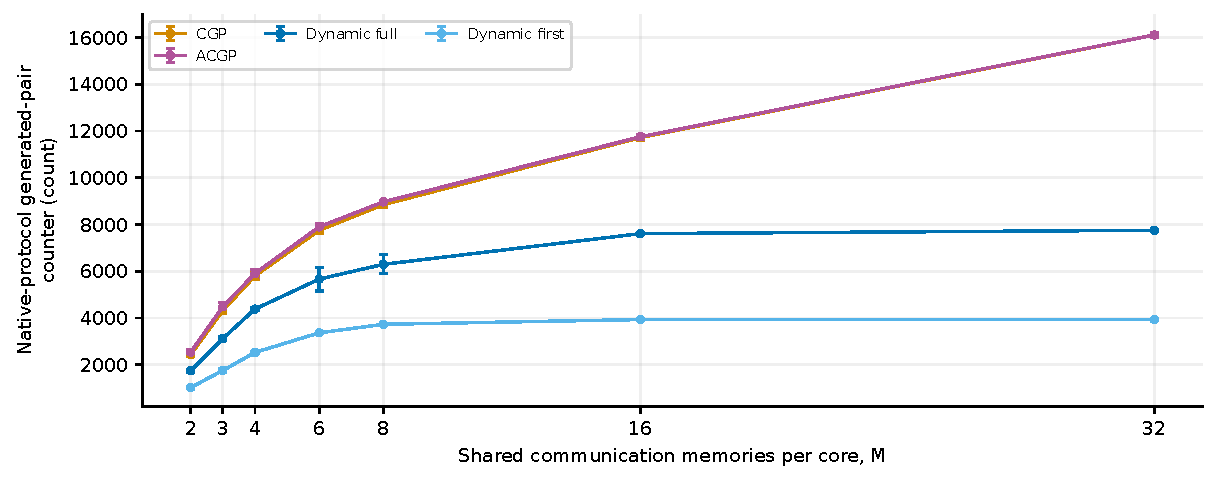
\includegraphics[width=.94\linewidth,height=.255\textheight,keepaspectratio]{figures/memory/mesh_shortest_reliable_protocol_generated_pairs.pdf}\captionof{figure}{Run-level mean and sample SD. Shared trace aliases are counted once.}\end{center}
\begin{center}{\scriptsize\setlength{\tabcolsep}{3pt}
\begin{tabular}{lrrrrr}
\toprule
M & ODG & CGP & ACGP & Dynamic full & Dynamic first \\
\midrule
2 & n/a & $2429.33\pm80.19$ & $2532.67\pm103.77$ & $1740.67\pm67.93$ & $1020.33\pm52.14$ \\
3 & n/a & $4318.67\pm125.64$ & $4478.00\pm189.63$ & $3117.00\pm64.99$ & $1750.00\pm67.54$ \\
4 & n/a & $5798.00\pm157.11$ & $5902.00\pm157.36$ & $4376.67\pm62.77$ & $2522.00\pm44.76$ \\
6 & n/a & $7752.33\pm121.27$ & $7898.00\pm122.64$ & $5661.00\pm508.95$ & $3362.00\pm43.12$ \\
8 & n/a & $8846.33\pm109.12$ & $8968.00\pm73.64$ & $6293.67\pm411.75$ & $3726.00\pm42.86$ \\
16 & n/a & $11719.33\pm114.94$ & $11751.67\pm112.46$ & $7608.00\pm53.56$ & $3930.00\pm0.00$ \\
32 & n/a & $16112.00\pm60.99$ & $16111.33\pm112.67$ & $7752.00\pm0.00$ & $3930.00\pm0.00$ \\
\bottomrule\end{tabular}}
\captionof{table}{Mean $\pm$ sample SD; n/a denotes a metric outside that policy's instrumentation.}
{\footnotesize\href{https://github.com/sanjeevkrishnaa/Compiler-Driven-ACE/blob/codex/ace-scheduler-correctness/docs/latex/qft96_final/data/memory_mesh_shortest_reliable_protocol_generated_pairs.csv}{Exact CSV values and sample counts}}
\end{center}
\clearpage
\subsection*{Native-protocol used-pair counter}
\begin{center}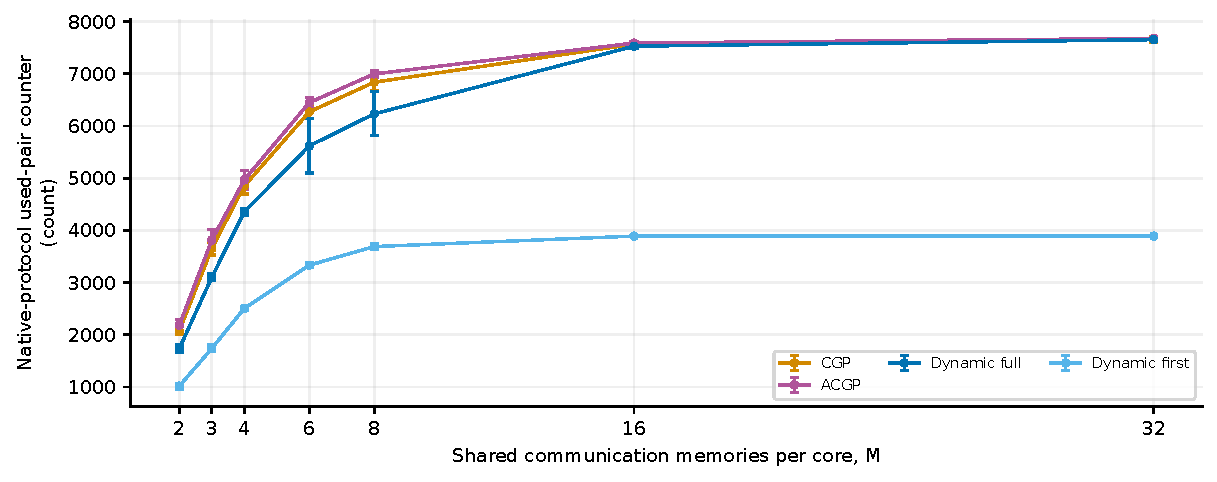
\includegraphics[width=.94\linewidth,height=.255\textheight,keepaspectratio]{figures/memory/mesh_shortest_reliable_protocol_used_pairs.pdf}\captionof{figure}{Run-level mean and sample SD. Shared trace aliases are counted once.}\end{center}
\begin{center}{\scriptsize\setlength{\tabcolsep}{3pt}
\begin{tabular}{lrrrrr}
\toprule
M & ODG & CGP & ACGP & Dynamic full & Dynamic first \\
\midrule
2 & n/a & $2073.33\pm76.59$ & $2182.67\pm102.42$ & $1734.67\pm69.21$ & $1015.00\pm54.31$ \\
3 & n/a & $3652.33\pm123.99$ & $3814.33\pm203.83$ & $3100.67\pm66.12$ & $1737.67\pm66.10$ \\
4 & n/a & $4850.00\pm152.65$ & $4967.33\pm175.54$ & $4355.33\pm61.11$ & $2504.67\pm42.89$ \\
6 & n/a & $6271.00\pm129.71$ & $6447.67\pm102.21$ & $5618.33\pm519.56$ & $3332.00\pm48.58$ \\
8 & n/a & $6839.00\pm158.87$ & $6998.00\pm60.37$ & $6232.67\pm420.75$ & $3689.33\pm49.08$ \\
16 & n/a & $7569.00\pm48.16$ & $7589.33\pm34.86$ & $7529.33\pm51.02$ & $3890.33\pm11.55$ \\
32 & n/a & $7656.33\pm51.22$ & $7678.67\pm22.44$ & $7654.33\pm8.24$ & $3890.33\pm11.55$ \\
\bottomrule\end{tabular}}
\captionof{table}{Mean $\pm$ sample SD; n/a denotes a metric outside that policy's instrumentation.}
{\footnotesize\href{https://github.com/sanjeevkrishnaa/Compiler-Driven-ACE/blob/codex/ace-scheduler-correctness/docs/latex/qft96_final/data/memory_mesh_shortest_reliable_protocol_used_pairs.csv}{Exact CSV values and sample counts}}
\end{center}
\subsection*{Native-protocol unused-pair counter}
\begin{center}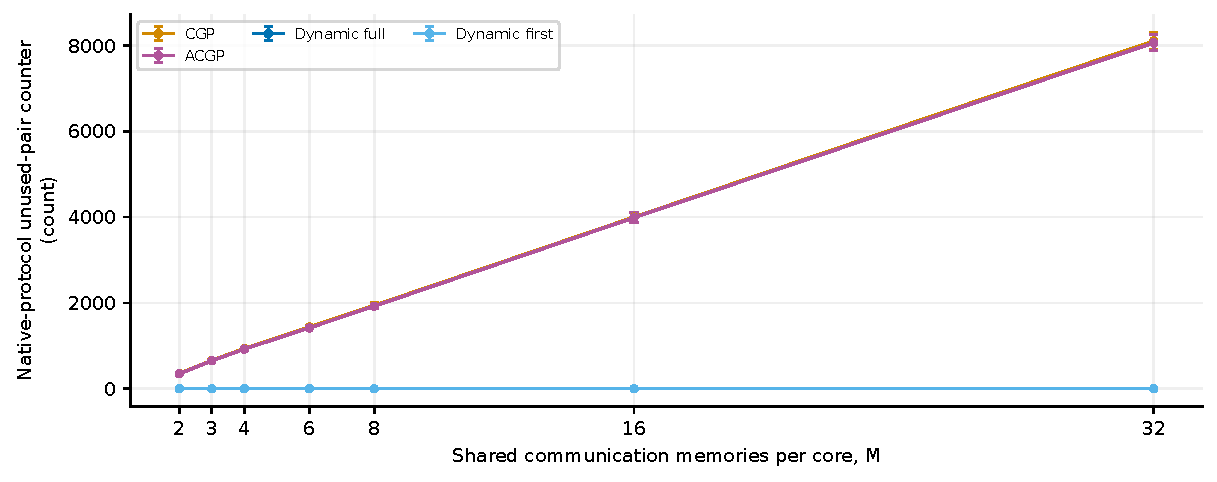
\includegraphics[width=.94\linewidth,height=.255\textheight,keepaspectratio]{figures/memory/mesh_shortest_reliable_protocol_unused_pairs.pdf}\captionof{figure}{Run-level mean and sample SD. Shared trace aliases are counted once.}\end{center}
\begin{center}{\scriptsize\setlength{\tabcolsep}{3pt}
\begin{tabular}{lrrrrr}
\toprule
M & ODG & CGP & ACGP & Dynamic full & Dynamic first \\
\midrule
2 & n/a & $353.33\pm10.41$ & $348.00\pm2.19$ & $0.0000\pm0.0000$ & $0.0000\pm0.0000$ \\
3 & n/a & $658.00\pm15.39$ & $651.33\pm16.86$ & $0.0000\pm0.0000$ & $0.0000\pm0.0000$ \\
4 & n/a & $936.33\pm21.96$ & $924.00\pm21.39$ & $0.0000\pm0.0000$ & $0.0000\pm0.0000$ \\
6 & n/a & $1437.67\pm33.88$ & $1417.00\pm12.88$ & $0.0000\pm0.0000$ & $0.0000\pm0.0000$ \\
8 & n/a & $1941.33\pm62.64$ & $1924.00\pm51.07$ & $0.0000\pm0.0000$ & $0.0000\pm0.0000$ \\
16 & n/a & $3999.33\pm114.57$ & $3987.67\pm120.58$ & $0.0000\pm0.0000$ & $0.0000\pm0.0000$ \\
32 & n/a & $8104.33\pm202.89$ & $8064.33\pm190.79$ & $0.0000\pm0.0000$ & $0.0000\pm0.0000$ \\
\bottomrule\end{tabular}}
\captionof{table}{Mean $\pm$ sample SD; n/a denotes a metric outside that policy's instrumentation.}
{\footnotesize\href{https://github.com/sanjeevkrishnaa/Compiler-Driven-ACE/blob/codex/ace-scheduler-correctness/docs/latex/qft96_final/data/memory_mesh_shortest_reliable_protocol_unused_pairs.csv}{Exact CSV values and sample counts}}
\end{center}
\clearpage
\subsection*{Scheduled compiler preparations}
\begin{center}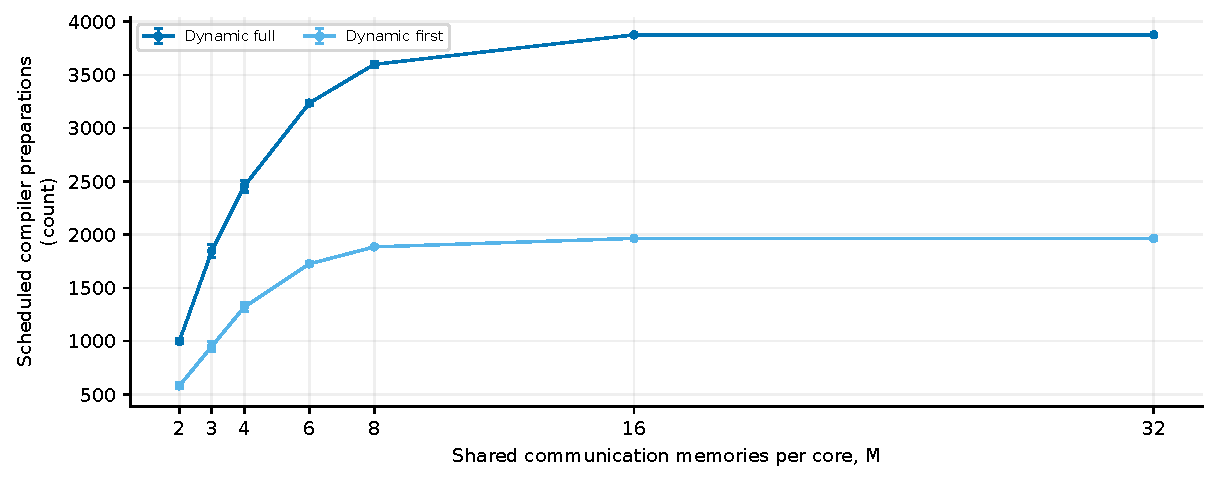
\includegraphics[width=.94\linewidth,height=.255\textheight,keepaspectratio]{figures/memory/mesh_shortest_reliable_scheduled_preparations.pdf}\captionof{figure}{Run-level mean and sample SD. Shared trace aliases are counted once.}\end{center}
\begin{center}{\scriptsize\setlength{\tabcolsep}{3pt}
\begin{tabular}{lrrrrr}
\toprule
M & ODG & CGP & ACGP & Dynamic full & Dynamic first \\
\midrule
2 & n/a & n/a & n/a & $999.00\pm24.93$ & $580.00\pm27.90$ \\
3 & n/a & n/a & n/a & $1846.33\pm57.91$ & $951.00\pm50.11$ \\
4 & n/a & n/a & n/a & $2455.67\pm55.36$ & $1320.33\pm38.55$ \\
6 & n/a & n/a & n/a & $3235.00\pm24.93$ & $1725.33\pm17.76$ \\
8 & n/a & n/a & n/a & $3598.67\pm30.27$ & $1885.00\pm8.81$ \\
16 & n/a & n/a & n/a & $3875.67\pm0.52$ & $1965.00\pm0.00$ \\
32 & n/a & n/a & n/a & $3876.00\pm0.00$ & $1965.00\pm0.00$ \\
\bottomrule\end{tabular}}
\captionof{table}{Mean $\pm$ sample SD; n/a denotes a metric outside that policy's instrumentation.}
{\footnotesize\href{https://github.com/sanjeevkrishnaa/Compiler-Driven-ACE/blob/codex/ace-scheduler-correctness/docs/latex/qft96_final/data/memory_mesh_shortest_reliable_scheduled_preparations.csv}{Exact CSV values and sample counts}}
\end{center}
\subsection*{Planner-blocked preparations}
\begin{center}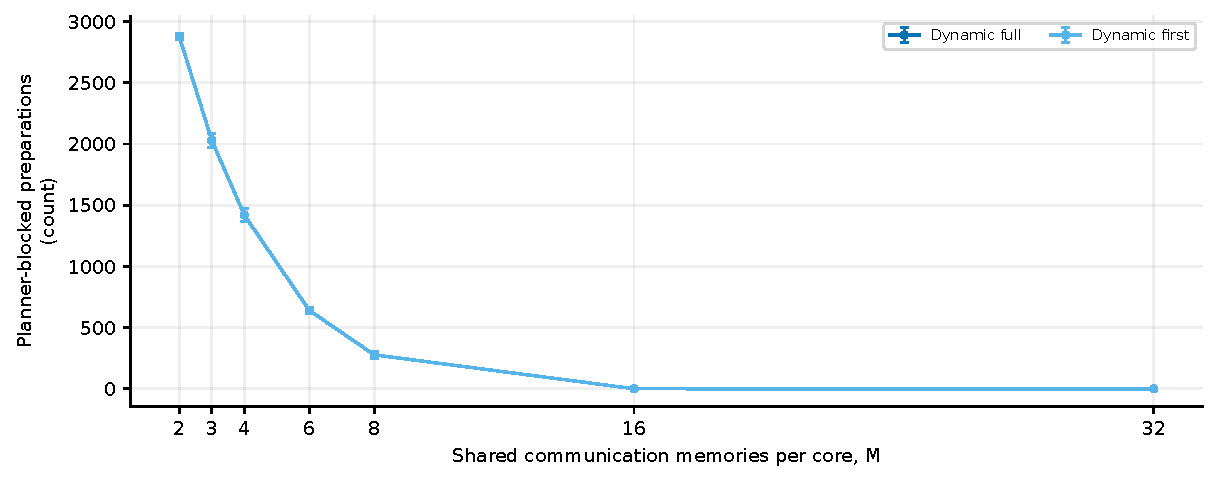
\includegraphics[width=.94\linewidth,height=.255\textheight,keepaspectratio]{figures/memory/mesh_shortest_reliable_planner_blocked_preparations.pdf}\captionof{figure}{Run-level mean and sample SD. Shared trace aliases are counted once.}\end{center}
\begin{center}{\scriptsize\setlength{\tabcolsep}{3pt}
\begin{tabular}{lrrrrr}
\toprule
M & ODG & CGP & ACGP & Dynamic full & Dynamic first \\
\midrule
2 & n/a & n/a & n/a & $2877.00\pm24.93$ & $2877.00\pm24.93$ \\
3 & n/a & n/a & n/a & $2029.67\pm57.91$ & $2029.67\pm57.91$ \\
4 & n/a & n/a & n/a & $1420.33\pm55.36$ & $1420.33\pm55.36$ \\
6 & n/a & n/a & n/a & $641.00\pm24.93$ & $641.00\pm24.93$ \\
8 & n/a & n/a & n/a & $277.33\pm30.27$ & $277.33\pm30.27$ \\
16 & n/a & n/a & n/a & $0.3333\pm0.5164$ & $0.3333\pm0.5164$ \\
32 & n/a & n/a & n/a & $0.0000\pm0.0000$ & $0.0000\pm0.0000$ \\
\bottomrule\end{tabular}}
\captionof{table}{Mean $\pm$ sample SD; n/a denotes a metric outside that policy's instrumentation.}
{\footnotesize\href{https://github.com/sanjeevkrishnaa/Compiler-Driven-ACE/blob/codex/ace-scheduler-correctness/docs/latex/qft96_final/data/memory_mesh_shortest_reliable_planner_blocked_preparations.csv}{Exact CSV values and sample counts}}
\end{center}
\clearpage
\subsection*{Planner peak compiler memory}
\begin{center}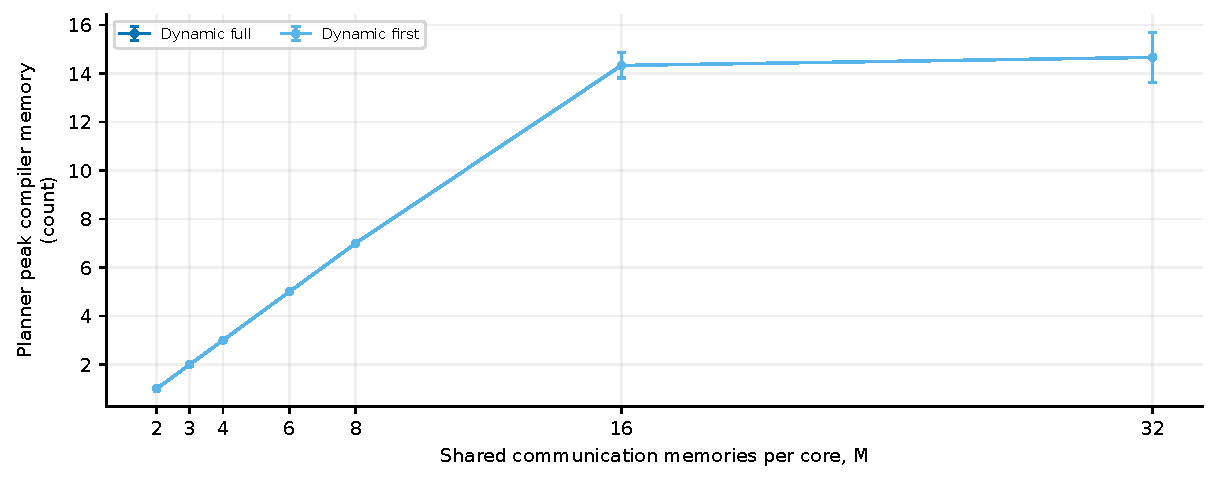
\includegraphics[width=.94\linewidth,height=.255\textheight,keepaspectratio]{figures/memory/mesh_shortest_reliable_planner_peak_compiler_memory_per_core.pdf}\captionof{figure}{Run-level mean and sample SD. Shared trace aliases are counted once.}\end{center}
\begin{center}{\scriptsize\setlength{\tabcolsep}{3pt}
\begin{tabular}{lrrrrr}
\toprule
M & ODG & CGP & ACGP & Dynamic full & Dynamic first \\
\midrule
2 & n/a & n/a & n/a & $1.000\pm0.000$ & $1.000\pm0.000$ \\
3 & n/a & n/a & n/a & $2.000\pm0.000$ & $2.000\pm0.000$ \\
4 & n/a & n/a & n/a & $3.000\pm0.000$ & $3.000\pm0.000$ \\
6 & n/a & n/a & n/a & $5.000\pm0.000$ & $5.000\pm0.000$ \\
8 & n/a & n/a & n/a & $7.000\pm0.000$ & $7.000\pm0.000$ \\
16 & n/a & n/a & n/a & $14.333\pm0.516$ & $14.333\pm0.516$ \\
32 & n/a & n/a & n/a & $14.667\pm1.033$ & $14.667\pm1.033$ \\
\bottomrule\end{tabular}}
\captionof{table}{Mean $\pm$ sample SD; n/a denotes a metric outside that policy's instrumentation.}
{\footnotesize\href{https://github.com/sanjeevkrishnaa/Compiler-Driven-ACE/blob/codex/ace-scheduler-correctness/docs/latex/qft96_final/data/memory_mesh_shortest_reliable_planner_peak_compiler_memory_per_core.csv}{Exact CSV values and sample counts}}
\end{center}
\subsection*{Compiler preparation admission attempts}
\begin{center}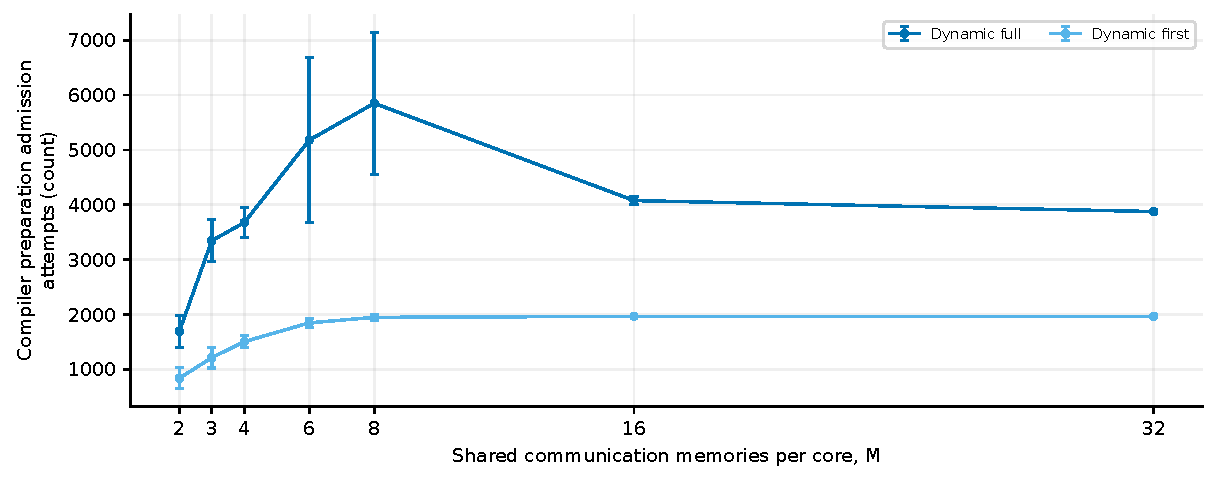
\includegraphics[width=.94\linewidth,height=.255\textheight,keepaspectratio]{figures/memory/mesh_shortest_reliable_runtime_admission_attempts.pdf}\captionof{figure}{Run-level mean and sample SD. Shared trace aliases are counted once.}\end{center}
\begin{center}{\scriptsize\setlength{\tabcolsep}{3pt}
\begin{tabular}{lrrrrr}
\toprule
M & ODG & CGP & ACGP & Dynamic full & Dynamic first \\
\midrule
2 & n/a & n/a & n/a & $1689.83\pm288.92$ & $834.00\pm190.08$ \\
3 & n/a & n/a & n/a & $3345.00\pm379.29$ & $1212.17\pm189.19$ \\
4 & n/a & n/a & n/a & $3676.00\pm273.67$ & $1502.67\pm113.90$ \\
6 & n/a & n/a & n/a & $5179.83\pm1502.58$ & $1845.83\pm76.55$ \\
8 & n/a & n/a & n/a & $5851.67\pm1294.63$ & $1946.50\pm49.09$ \\
16 & n/a & n/a & n/a & $4076.83\pm78.70$ & $1965.00\pm0.00$ \\
32 & n/a & n/a & n/a & $3876.00\pm0.00$ & $1965.00\pm0.00$ \\
\bottomrule\end{tabular}}
\captionof{table}{Mean $\pm$ sample SD; n/a denotes a metric outside that policy's instrumentation.}
{\footnotesize\href{https://github.com/sanjeevkrishnaa/Compiler-Driven-ACE/blob/codex/ace-scheduler-correctness/docs/latex/qft96_final/data/memory_mesh_shortest_reliable_runtime_admission_attempts.csv}{Exact CSV values and sample counts}}
\end{center}
\clearpage
\subsection*{Launched compiler preparations}
\begin{center}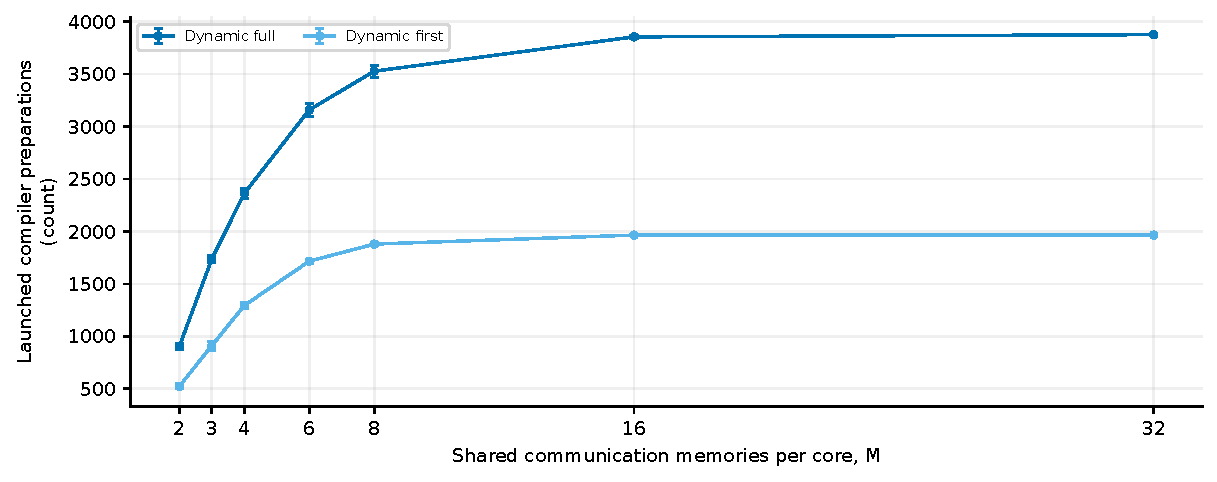
\includegraphics[width=.94\linewidth,height=.255\textheight,keepaspectratio]{figures/memory/mesh_shortest_reliable_runtime_launched_preparations.pdf}\captionof{figure}{Run-level mean and sample SD. Shared trace aliases are counted once.}\end{center}
\begin{center}{\scriptsize\setlength{\tabcolsep}{3pt}
\begin{tabular}{lrrrrr}
\toprule
M & ODG & CGP & ACGP & Dynamic full & Dynamic first \\
\midrule
2 & n/a & n/a & n/a & $903.67\pm26.24$ & $522.83\pm23.83$ \\
3 & n/a & n/a & n/a & $1736.50\pm35.84$ & $910.33\pm42.63$ \\
4 & n/a & n/a & n/a & $2362.67\pm44.62$ & $1293.67\pm29.38$ \\
6 & n/a & n/a & n/a & $3158.50\pm60.38$ & $1716.00\pm18.93$ \\
8 & n/a & n/a & n/a & $3527.50\pm56.72$ & $1879.17\pm13.35$ \\
16 & n/a & n/a & n/a & $3854.67\pm10.58$ & $1965.00\pm0.00$ \\
32 & n/a & n/a & n/a & $3876.00\pm0.00$ & $1965.00\pm0.00$ \\
\bottomrule\end{tabular}}
\captionof{table}{Mean $\pm$ sample SD; n/a denotes a metric outside that policy's instrumentation.}
{\footnotesize\href{https://github.com/sanjeevkrishnaa/Compiler-Driven-ACE/blob/codex/ace-scheduler-correctness/docs/latex/qft96_final/data/memory_mesh_shortest_reliable_runtime_launched_preparations.csv}{Exact CSV values and sample counts}}
\end{center}
\subsection*{Accepted compiler preparations}
\begin{center}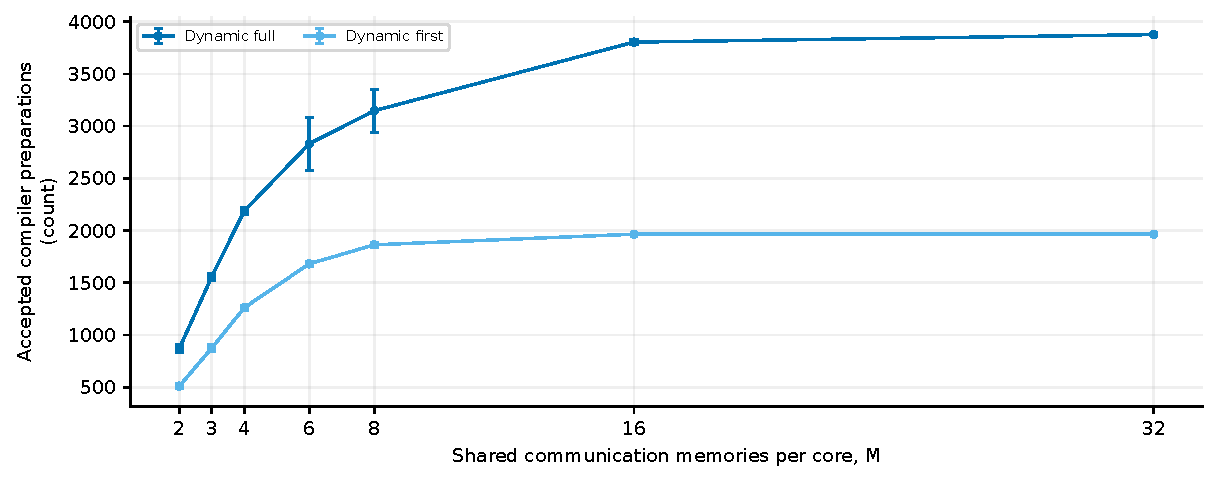
\includegraphics[width=.94\linewidth,height=.255\textheight,keepaspectratio]{figures/memory/mesh_shortest_reliable_runtime_accepted_preparations.pdf}\captionof{figure}{Run-level mean and sample SD. Shared trace aliases are counted once.}\end{center}
\begin{center}{\scriptsize\setlength{\tabcolsep}{3pt}
\begin{tabular}{lrrrrr}
\toprule
M & ODG & CGP & ACGP & Dynamic full & Dynamic first \\
\midrule
2 & n/a & n/a & n/a & $870.33\pm33.96$ & $510.17\pm26.07$ \\
3 & n/a & n/a & n/a & $1558.50\pm32.49$ & $875.00\pm33.77$ \\
4 & n/a & n/a & n/a & $2188.33\pm31.39$ & $1261.00\pm22.38$ \\
6 & n/a & n/a & n/a & $2830.50\pm254.47$ & $1681.00\pm21.56$ \\
8 & n/a & n/a & n/a & $3146.83\pm205.87$ & $1863.00\pm21.43$ \\
16 & n/a & n/a & n/a & $3804.00\pm26.78$ & $1965.00\pm0.00$ \\
32 & n/a & n/a & n/a & $3876.00\pm0.00$ & $1965.00\pm0.00$ \\
\bottomrule\end{tabular}}
\captionof{table}{Mean $\pm$ sample SD; n/a denotes a metric outside that policy's instrumentation.}
{\footnotesize\href{https://github.com/sanjeevkrishnaa/Compiler-Driven-ACE/blob/codex/ace-scheduler-correctness/docs/latex/qft96_final/data/memory_mesh_shortest_reliable_runtime_accepted_preparations.csv}{Exact CSV values and sample counts}}
\end{center}
\clearpage
\subsection*{Rejected compiler preparations}
\begin{center}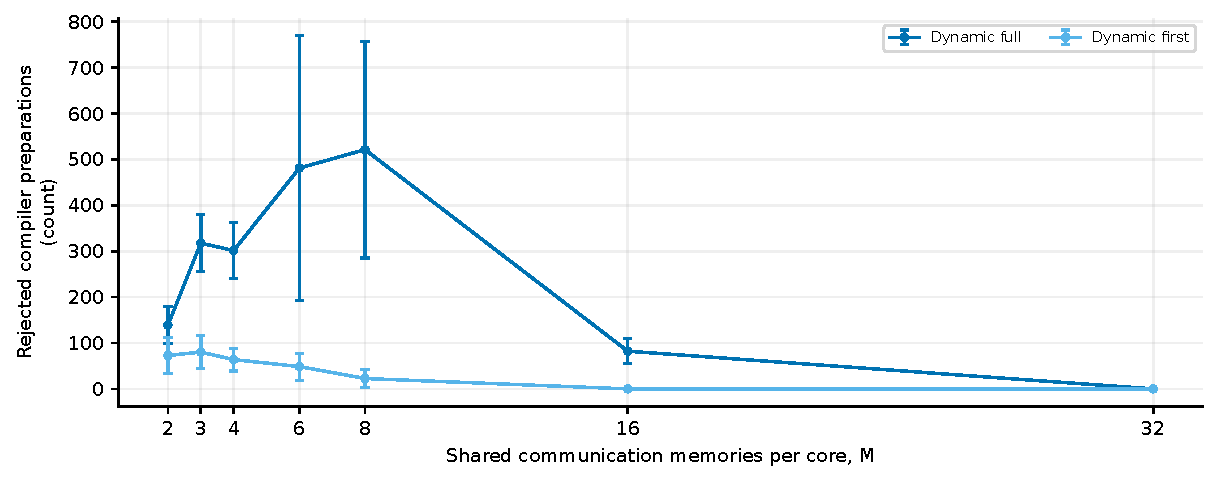
\includegraphics[width=.94\linewidth,height=.255\textheight,keepaspectratio]{figures/memory/mesh_shortest_reliable_runtime_rejected_preparations.pdf}\captionof{figure}{Run-level mean and sample SD. Shared trace aliases are counted once.}\end{center}
\begin{center}{\scriptsize\setlength{\tabcolsep}{3pt}
\begin{tabular}{lrrrrr}
\toprule
M & ODG & CGP & ACGP & Dynamic full & Dynamic first \\
\midrule
2 & n/a & n/a & n/a & $139.00\pm40.42$ & $72.833\pm38.603$ \\
3 & n/a & n/a & n/a & $317.50\pm62.48$ & $80.167\pm35.830$ \\
4 & n/a & n/a & n/a & $301.33\pm61.52$ & $63.833\pm24.871$ \\
6 & n/a & n/a & n/a & $481.00\pm288.04$ & $48.667\pm29.385$ \\
8 & n/a & n/a & n/a & $521.17\pm236.10$ & $22.667\pm19.054$ \\
16 & n/a & n/a & n/a & $82.167\pm27.147$ & $0.0000\pm0.0000$ \\
32 & n/a & n/a & n/a & $0.0000\pm0.0000$ & $0.0000\pm0.0000$ \\
\bottomrule\end{tabular}}
\captionof{table}{Mean $\pm$ sample SD; n/a denotes a metric outside that policy's instrumentation.}
{\footnotesize\href{https://github.com/sanjeevkrishnaa/Compiler-Driven-ACE/blob/codex/ace-scheduler-correctness/docs/latex/qft96_final/data/memory_mesh_shortest_reliable_runtime_rejected_preparations.csv}{Exact CSV values and sample counts}}
\end{center}
\subsection*{Compiler-ready request count}
\begin{center}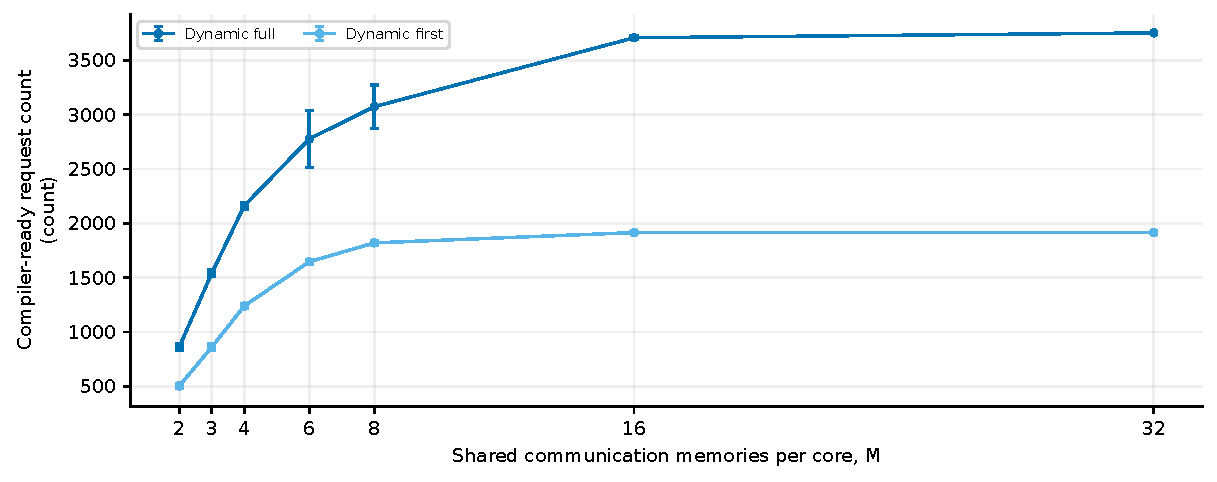
\includegraphics[width=.94\linewidth,height=.255\textheight,keepaspectratio]{figures/memory/mesh_shortest_reliable_pregenerated_hits.pdf}\captionof{figure}{Run-level mean and sample SD. Shared trace aliases are counted once.}\end{center}
\begin{center}{\scriptsize\setlength{\tabcolsep}{3pt}
\begin{tabular}{lrrrrr}
\toprule
M & ODG & CGP & ACGP & Dynamic full & Dynamic first \\
\midrule
2 & n/a & n/a & n/a & $862.67\pm33.61$ & $503.33\pm26.06$ \\
3 & n/a & n/a & n/a & $1541.17\pm32.71$ & $860.67\pm32.18$ \\
4 & n/a & n/a & n/a & $2161.83\pm32.62$ & $1239.33\pm24.30$ \\
6 & n/a & n/a & n/a & $2777.17\pm261.05$ & $1645.83\pm22.49$ \\
8 & n/a & n/a & n/a & $3073.50\pm199.98$ & $1819.83\pm23.16$ \\
16 & n/a & n/a & n/a & $3708.00\pm18.97$ & $1914.83\pm6.11$ \\
32 & n/a & n/a & n/a & $3753.17\pm5.04$ & $1914.83\pm6.11$ \\
\bottomrule\end{tabular}}
\captionof{table}{Mean $\pm$ sample SD; n/a denotes a metric outside that policy's instrumentation.}
{\footnotesize\href{https://github.com/sanjeevkrishnaa/Compiler-Driven-ACE/blob/codex/ace-scheduler-correctness/docs/latex/qft96_final/data/memory_mesh_shortest_reliable_pregenerated_hits.csv}{Exact CSV values and sample counts}}
\end{center}
\clearpage
\subsection*{Intended compiler-hit count}
\begin{center}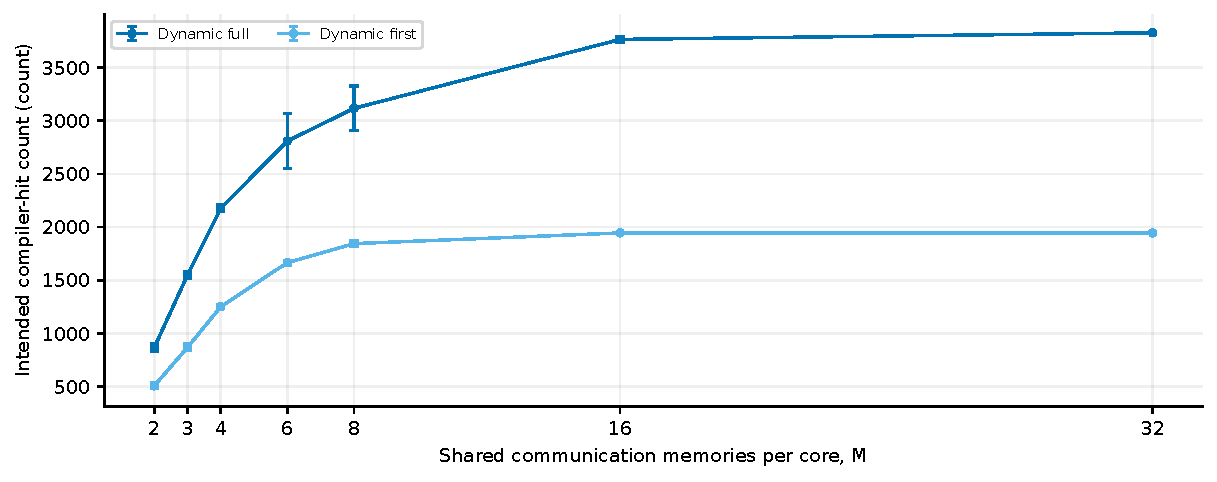
\includegraphics[width=.94\linewidth,height=.255\textheight,keepaspectratio]{figures/memory/mesh_shortest_reliable_intended_request_hits.pdf}\captionof{figure}{Run-level mean and sample SD. Shared trace aliases are counted once.}\end{center}
\begin{center}{\scriptsize\setlength{\tabcolsep}{3pt}
\begin{tabular}{lrrrrr}
\toprule
M & ODG & CGP & ACGP & Dynamic full & Dynamic first \\
\midrule
2 & n/a & n/a & n/a & $867.33\pm34.60$ & $507.50\pm27.16$ \\
3 & n/a & n/a & n/a & $1550.33\pm33.06$ & $868.83\pm33.05$ \\
4 & n/a & n/a & n/a & $2177.67\pm30.55$ & $1252.33\pm21.44$ \\
6 & n/a & n/a & n/a & $2809.17\pm259.78$ & $1666.00\pm24.29$ \\
8 & n/a & n/a & n/a & $3116.33\pm210.37$ & $1844.67\pm24.54$ \\
16 & n/a & n/a & n/a & $3764.67\pm25.51$ & $1945.17\pm5.78$ \\
32 & n/a & n/a & n/a & $3827.17\pm4.12$ & $1945.17\pm5.78$ \\
\bottomrule\end{tabular}}
\captionof{table}{Mean $\pm$ sample SD; n/a denotes a metric outside that policy's instrumentation.}
{\footnotesize\href{https://github.com/sanjeevkrishnaa/Compiler-Driven-ACE/blob/codex/ace-scheduler-correctness/docs/latex/qft96_final/data/memory_mesh_shortest_reliable_intended_request_hits.csv}{Exact CSV values and sample counts}}
\end{center}
\subsection*{Compiler-not-ready request count}
\begin{center}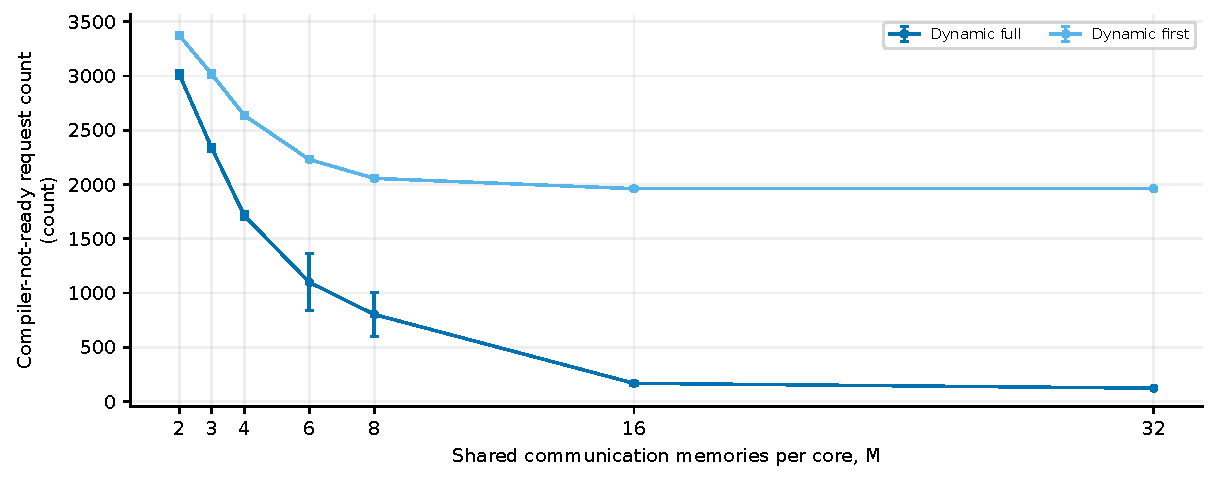
\includegraphics[width=.94\linewidth,height=.255\textheight,keepaspectratio]{figures/memory/mesh_shortest_reliable_compiler_not_ready_requests.pdf}\captionof{figure}{Run-level mean and sample SD. Shared trace aliases are counted once.}\end{center}
\begin{center}{\scriptsize\setlength{\tabcolsep}{3pt}
\begin{tabular}{lrrrrr}
\toprule
M & ODG & CGP & ACGP & Dynamic full & Dynamic first \\
\midrule
2 & n/a & n/a & n/a & $3013.33\pm33.61$ & $3372.67\pm26.06$ \\
3 & n/a & n/a & n/a & $2334.83\pm32.71$ & $3015.33\pm32.18$ \\
4 & n/a & n/a & n/a & $1714.17\pm32.62$ & $2636.67\pm24.30$ \\
6 & n/a & n/a & n/a & $1098.83\pm261.05$ & $2230.17\pm22.49$ \\
8 & n/a & n/a & n/a & $802.50\pm199.98$ & $2056.17\pm23.16$ \\
16 & n/a & n/a & n/a & $168.00\pm18.97$ & $1961.17\pm6.11$ \\
32 & n/a & n/a & n/a & $122.83\pm5.04$ & $1961.17\pm6.11$ \\
\bottomrule\end{tabular}}
\captionof{table}{Mean $\pm$ sample SD; n/a denotes a metric outside that policy's instrumentation.}
{\footnotesize\href{https://github.com/sanjeevkrishnaa/Compiler-Driven-ACE/blob/codex/ace-scheduler-correctness/docs/latex/qft96_final/data/memory_mesh_shortest_reliable_compiler_not_ready_requests.csv}{Exact CSV values and sample counts}}
\end{center}
\clearpage
\subsection*{Late compiler-pair uses}
\begin{center}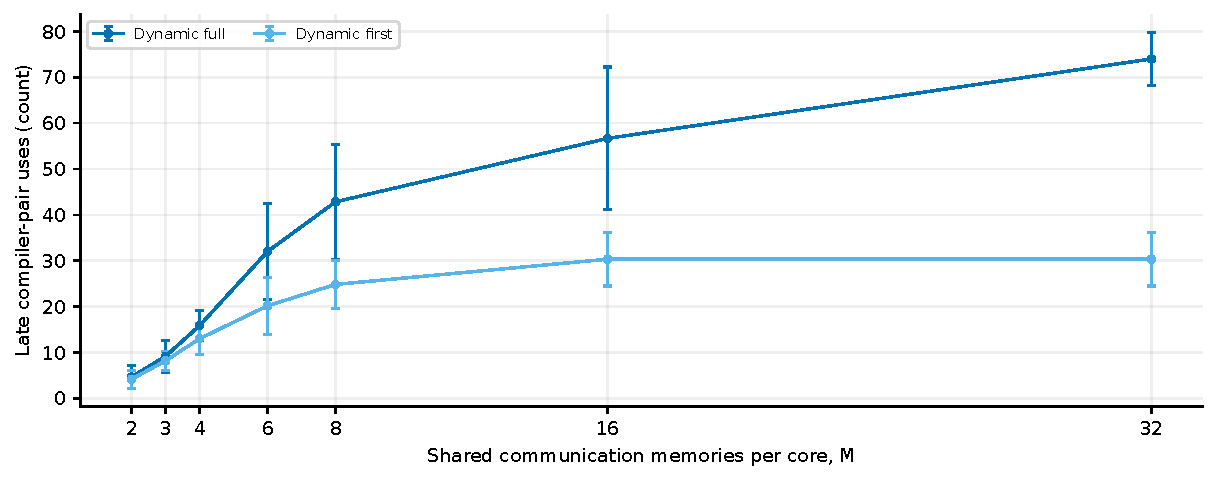
\includegraphics[width=.94\linewidth,height=.255\textheight,keepaspectratio]{figures/memory/mesh_shortest_reliable_late_compiler_pair_uses.pdf}\captionof{figure}{Run-level mean and sample SD. Shared trace aliases are counted once.}\end{center}
\begin{center}{\scriptsize\setlength{\tabcolsep}{3pt}
\begin{tabular}{lrrrrr}
\toprule
M & ODG & CGP & ACGP & Dynamic full & Dynamic first \\
\midrule
2 & n/a & n/a & n/a & $4.667\pm2.582$ & $4.167\pm1.941$ \\
3 & n/a & n/a & n/a & $9.167\pm3.430$ & $8.167\pm2.137$ \\
4 & n/a & n/a & n/a & $15.833\pm3.251$ & $13.000\pm3.406$ \\
6 & n/a & n/a & n/a & $32.000\pm10.545$ & $20.167\pm6.178$ \\
8 & n/a & n/a & n/a & $42.833\pm12.561$ & $24.833\pm5.307$ \\
16 & n/a & n/a & n/a & $56.667\pm15.565$ & $30.333\pm5.854$ \\
32 & n/a & n/a & n/a & $74.000\pm5.797$ & $30.333\pm5.854$ \\
\bottomrule\end{tabular}}
\captionof{table}{Mean $\pm$ sample SD; n/a denotes a metric outside that policy's instrumentation.}
{\footnotesize\href{https://github.com/sanjeevkrishnaa/Compiler-Driven-ACE/blob/codex/ace-scheduler-correctness/docs/latex/qft96_final/data/memory_mesh_shortest_reliable_late_compiler_pair_uses.csv}{Exact CSV values and sample counts}}
\end{center}
\subsection*{Compiler fallback count}
\begin{center}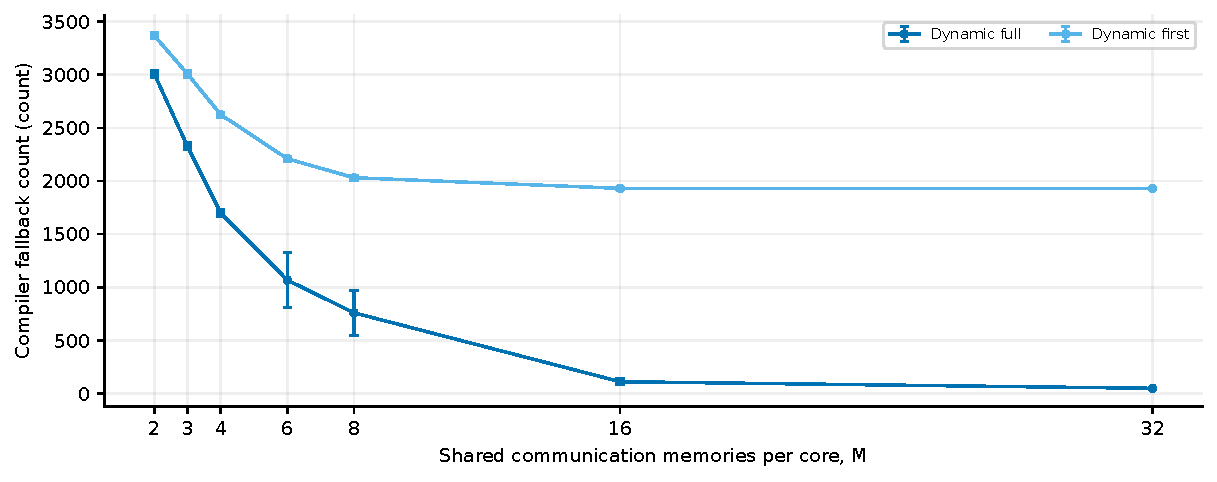
\includegraphics[width=.94\linewidth,height=.255\textheight,keepaspectratio]{figures/memory/mesh_shortest_reliable_on_demand_fallbacks.pdf}\captionof{figure}{Run-level mean and sample SD. Shared trace aliases are counted once.}\end{center}
\begin{center}{\scriptsize\setlength{\tabcolsep}{3pt}
\begin{tabular}{lrrrrr}
\toprule
M & ODG & CGP & ACGP & Dynamic full & Dynamic first \\
\midrule
2 & n/a & n/a & n/a & $3008.67\pm34.60$ & $3368.50\pm27.16$ \\
3 & n/a & n/a & n/a & $2325.67\pm33.06$ & $3007.17\pm33.05$ \\
4 & n/a & n/a & n/a & $1698.33\pm30.55$ & $2623.67\pm21.44$ \\
6 & n/a & n/a & n/a & $1066.83\pm259.78$ & $2210.00\pm24.29$ \\
8 & n/a & n/a & n/a & $759.67\pm210.37$ & $2031.33\pm24.54$ \\
16 & n/a & n/a & n/a & $111.33\pm25.51$ & $1930.83\pm5.78$ \\
32 & n/a & n/a & n/a & $48.833\pm4.119$ & $1930.83\pm5.78$ \\
\bottomrule\end{tabular}}
\captionof{table}{Mean $\pm$ sample SD; n/a denotes a metric outside that policy's instrumentation.}
{\footnotesize\href{https://github.com/sanjeevkrishnaa/Compiler-Driven-ACE/blob/codex/ace-scheduler-correctness/docs/latex/qft96_final/data/memory_mesh_shortest_reliable_on_demand_fallbacks.csv}{Exact CSV values and sample counts}}
\end{center}
\clearpage
\subsection*{Generated compiler pairs}
\begin{center}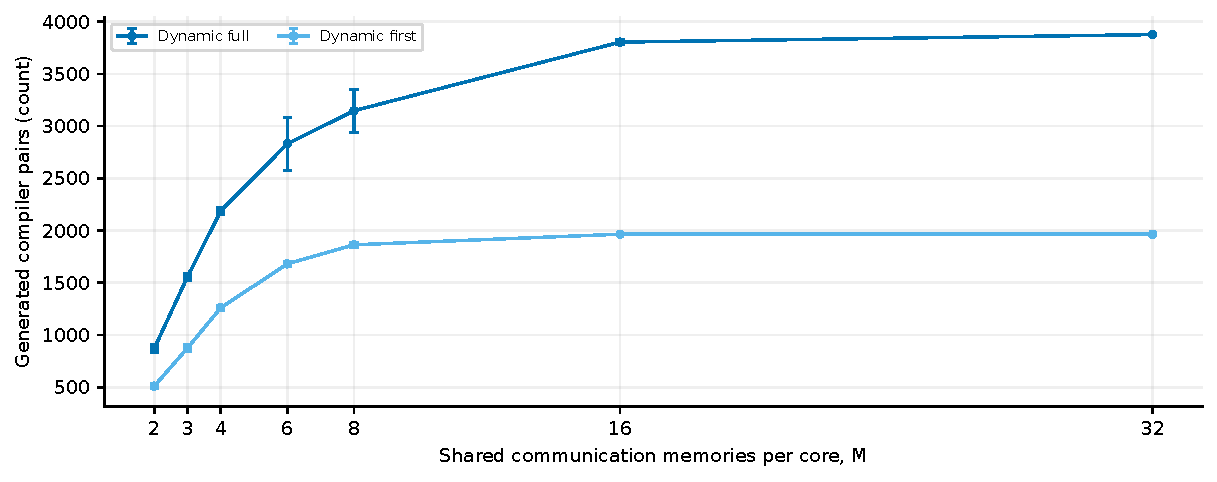
\includegraphics[width=.94\linewidth,height=.255\textheight,keepaspectratio]{figures/memory/mesh_shortest_reliable_generated_compiler_pairs.pdf}\captionof{figure}{Run-level mean and sample SD. Shared trace aliases are counted once.}\end{center}
\begin{center}{\scriptsize\setlength{\tabcolsep}{3pt}
\begin{tabular}{lrrrrr}
\toprule
M & ODG & CGP & ACGP & Dynamic full & Dynamic first \\
\midrule
2 & n/a & n/a & n/a & $870.33\pm33.96$ & $510.17\pm26.07$ \\
3 & n/a & n/a & n/a & $1558.50\pm32.49$ & $875.00\pm33.77$ \\
4 & n/a & n/a & n/a & $2188.33\pm31.39$ & $1261.00\pm22.38$ \\
6 & n/a & n/a & n/a & $2830.50\pm254.47$ & $1681.00\pm21.56$ \\
8 & n/a & n/a & n/a & $3146.83\pm205.87$ & $1863.00\pm21.43$ \\
16 & n/a & n/a & n/a & $3804.00\pm26.78$ & $1965.00\pm0.00$ \\
32 & n/a & n/a & n/a & $3876.00\pm0.00$ & $1965.00\pm0.00$ \\
\bottomrule\end{tabular}}
\captionof{table}{Mean $\pm$ sample SD; n/a denotes a metric outside that policy's instrumentation.}
{\footnotesize\href{https://github.com/sanjeevkrishnaa/Compiler-Driven-ACE/blob/codex/ace-scheduler-correctness/docs/latex/qft96_final/data/memory_mesh_shortest_reliable_generated_compiler_pairs.csv}{Exact CSV values and sample counts}}
\end{center}
\subsection*{Used compiler pairs}
\begin{center}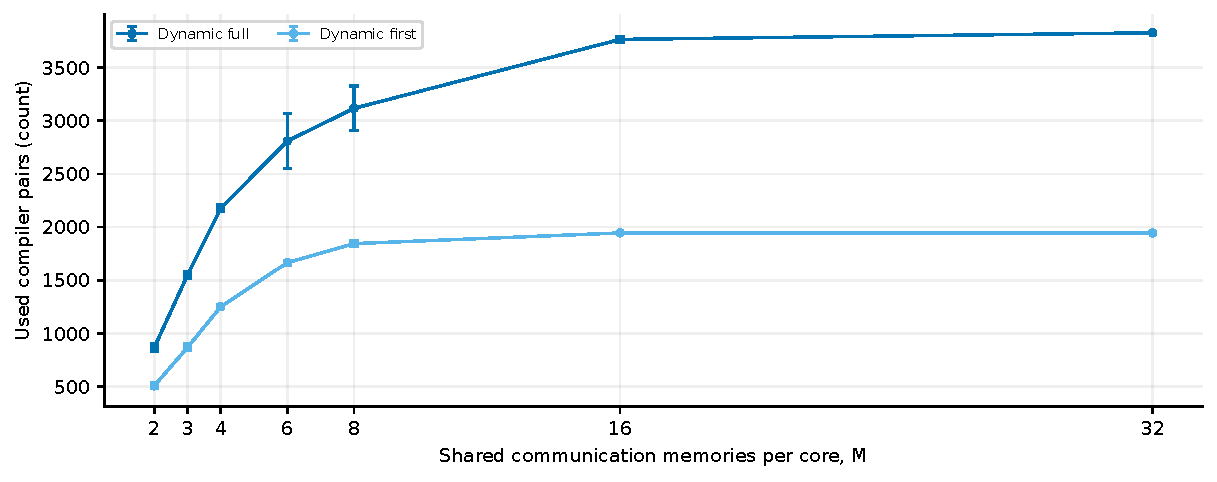
\includegraphics[width=.94\linewidth,height=.255\textheight,keepaspectratio]{figures/memory/mesh_shortest_reliable_utilized_compiler_pairs.pdf}\captionof{figure}{Run-level mean and sample SD. Shared trace aliases are counted once.}\end{center}
\begin{center}{\scriptsize\setlength{\tabcolsep}{3pt}
\begin{tabular}{lrrrrr}
\toprule
M & ODG & CGP & ACGP & Dynamic full & Dynamic first \\
\midrule
2 & n/a & n/a & n/a & $867.33\pm34.60$ & $507.50\pm27.16$ \\
3 & n/a & n/a & n/a & $1550.33\pm33.06$ & $868.83\pm33.05$ \\
4 & n/a & n/a & n/a & $2177.67\pm30.55$ & $1252.33\pm21.44$ \\
6 & n/a & n/a & n/a & $2809.17\pm259.78$ & $1666.00\pm24.29$ \\
8 & n/a & n/a & n/a & $3116.33\pm210.37$ & $1844.67\pm24.54$ \\
16 & n/a & n/a & n/a & $3764.67\pm25.51$ & $1945.17\pm5.78$ \\
32 & n/a & n/a & n/a & $3827.17\pm4.12$ & $1945.17\pm5.78$ \\
\bottomrule\end{tabular}}
\captionof{table}{Mean $\pm$ sample SD; n/a denotes a metric outside that policy's instrumentation.}
{\footnotesize\href{https://github.com/sanjeevkrishnaa/Compiler-Driven-ACE/blob/codex/ace-scheduler-correctness/docs/latex/qft96_final/data/memory_mesh_shortest_reliable_utilized_compiler_pairs.csv}{Exact CSV values and sample counts}}
\end{center}
\clearpage
\subsection*{Expired compiler pairs}
\begin{center}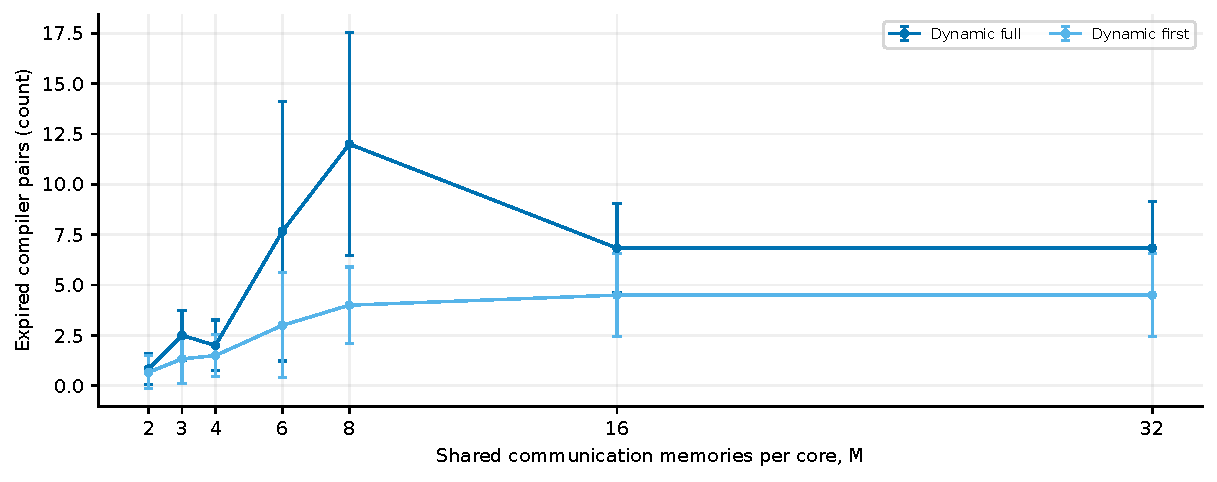
\includegraphics[width=.94\linewidth,height=.255\textheight,keepaspectratio]{figures/memory/mesh_shortest_reliable_expired_compiler_pairs.pdf}\captionof{figure}{Run-level mean and sample SD. Shared trace aliases are counted once.}\end{center}
\begin{center}{\scriptsize\setlength{\tabcolsep}{3pt}
\begin{tabular}{lrrrrr}
\toprule
M & ODG & CGP & ACGP & Dynamic full & Dynamic first \\
\midrule
2 & n/a & n/a & n/a & $0.8333\pm0.7528$ & $0.6667\pm0.8165$ \\
3 & n/a & n/a & n/a & $2.500\pm1.225$ & $1.333\pm1.211$ \\
4 & n/a & n/a & n/a & $2.000\pm1.265$ & $1.500\pm1.049$ \\
6 & n/a & n/a & n/a & $7.667\pm6.439$ & $3.000\pm2.608$ \\
8 & n/a & n/a & n/a & $12.000\pm5.550$ & $4.000\pm1.897$ \\
16 & n/a & n/a & n/a & $6.833\pm2.229$ & $4.500\pm2.074$ \\
32 & n/a & n/a & n/a & $6.833\pm2.317$ & $4.500\pm2.074$ \\
\bottomrule\end{tabular}}
\captionof{table}{Mean $\pm$ sample SD; n/a denotes a metric outside that policy's instrumentation.}
{\footnotesize\href{https://github.com/sanjeevkrishnaa/Compiler-Driven-ACE/blob/codex/ace-scheduler-correctness/docs/latex/qft96_final/data/memory_mesh_shortest_reliable_expired_compiler_pairs.csv}{Exact CSV values and sample counts}}
\end{center}
\subsection*{Remaining compiler pairs}
\begin{center}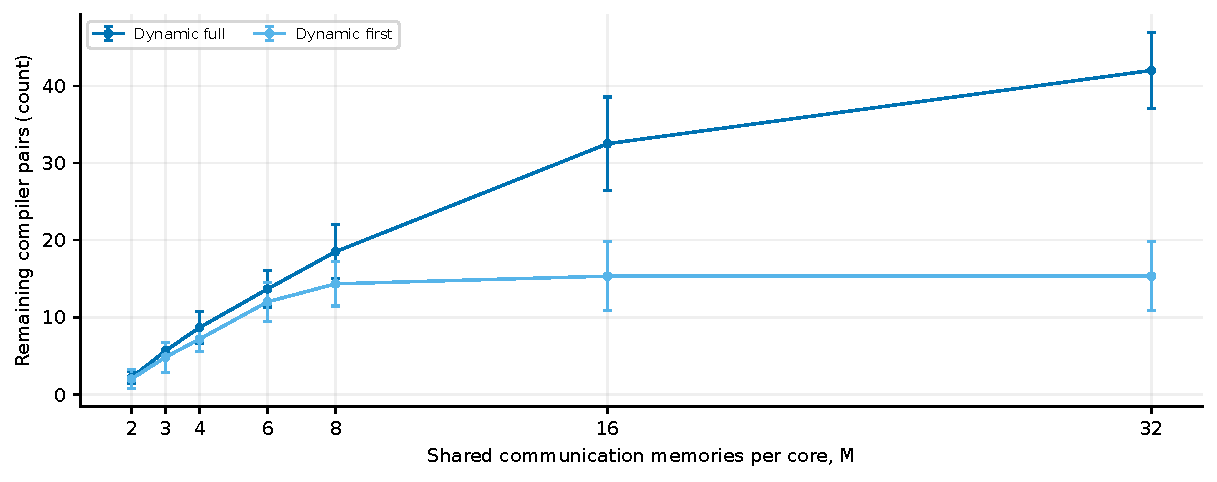
\includegraphics[width=.94\linewidth,height=.255\textheight,keepaspectratio]{figures/memory/mesh_shortest_reliable_remaining_compiler_pairs.pdf}\captionof{figure}{Run-level mean and sample SD. Shared trace aliases are counted once.}\end{center}
\begin{center}{\scriptsize\setlength{\tabcolsep}{3pt}
\begin{tabular}{lrrrrr}
\toprule
M & ODG & CGP & ACGP & Dynamic full & Dynamic first \\
\midrule
2 & n/a & n/a & n/a & $2.167\pm0.753$ & $2.000\pm1.265$ \\
3 & n/a & n/a & n/a & $5.667\pm1.033$ & $4.833\pm1.941$ \\
4 & n/a & n/a & n/a & $8.667\pm2.066$ & $7.167\pm1.602$ \\
6 & n/a & n/a & n/a & $13.667\pm2.338$ & $12.000\pm2.530$ \\
8 & n/a & n/a & n/a & $18.500\pm3.507$ & $14.333\pm2.875$ \\
16 & n/a & n/a & n/a & $32.500\pm6.058$ & $15.333\pm4.502$ \\
32 & n/a & n/a & n/a & $42.000\pm4.940$ & $15.333\pm4.502$ \\
\bottomrule\end{tabular}}
\captionof{table}{Mean $\pm$ sample SD; n/a denotes a metric outside that policy's instrumentation.}
{\footnotesize\href{https://github.com/sanjeevkrishnaa/Compiler-Driven-ACE/blob/codex/ace-scheduler-correctness/docs/latex/qft96_final/data/memory_mesh_shortest_reliable_remaining_compiler_pairs.csv}{Exact CSV values and sample counts}}
\end{center}
\clearpage
\subsection*{Compiler fidelity at creation}
\begin{center}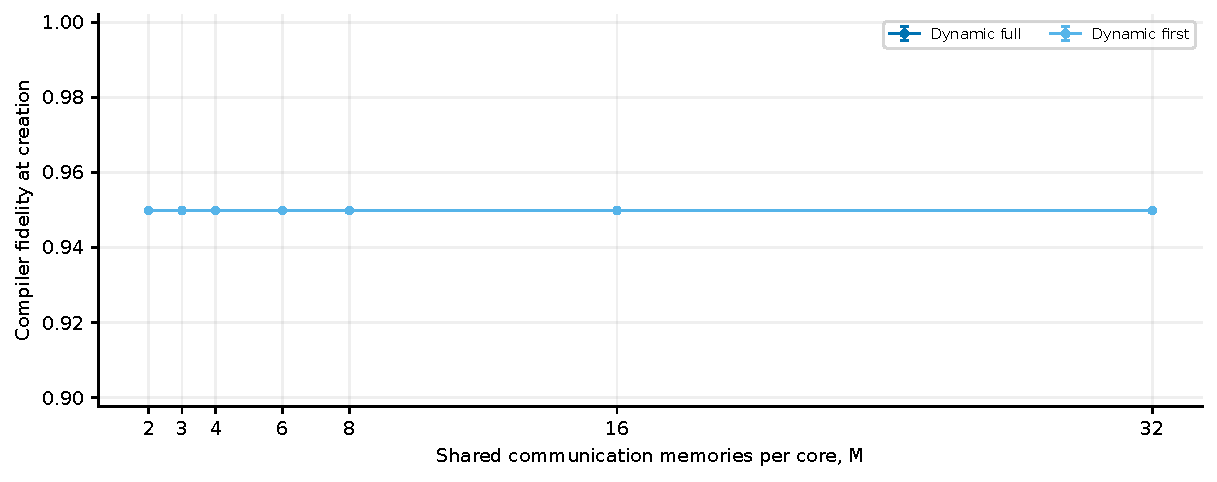
\includegraphics[width=.94\linewidth,height=.255\textheight,keepaspectratio]{figures/memory/mesh_shortest_reliable_average_fidelity_at_creation.pdf}\captionof{figure}{Run-level mean and sample SD. Shared trace aliases are counted once.}\end{center}
\begin{center}{\scriptsize\setlength{\tabcolsep}{3pt}
\begin{tabular}{lrrrrr}
\toprule
M & ODG & CGP & ACGP & Dynamic full & Dynamic first \\
\midrule
2 & n/a & n/a & n/a & $0.9498\pm0.0000$ & $0.9498\pm0.0000$ \\
3 & n/a & n/a & n/a & $0.9498\pm0.0000$ & $0.9498\pm0.0000$ \\
4 & n/a & n/a & n/a & $0.9498\pm0.0000$ & $0.9498\pm0.0000$ \\
6 & n/a & n/a & n/a & $0.9498\pm0.0000$ & $0.9498\pm0.0000$ \\
8 & n/a & n/a & n/a & $0.9498\pm0.0000$ & $0.9498\pm0.0000$ \\
16 & n/a & n/a & n/a & $0.9498\pm0.0000$ & $0.9498\pm0.0000$ \\
32 & n/a & n/a & n/a & $0.9498\pm0.0000$ & $0.9498\pm0.0000$ \\
\bottomrule\end{tabular}}
\captionof{table}{Mean $\pm$ sample SD; n/a denotes a metric outside that policy's instrumentation.}
{\footnotesize\href{https://github.com/sanjeevkrishnaa/Compiler-Driven-ACE/blob/codex/ace-scheduler-correctness/docs/latex/qft96_final/data/memory_mesh_shortest_reliable_average_fidelity_at_creation.csv}{Exact CSV values and sample counts}}
\end{center}
\subsection*{Compiler fidelity at use}
\begin{center}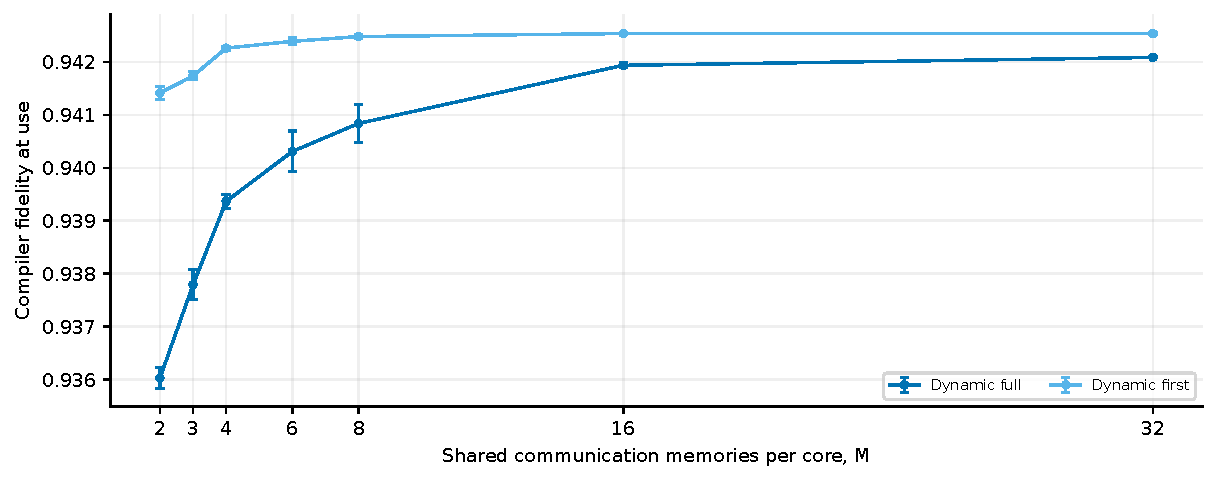
\includegraphics[width=.94\linewidth,height=.255\textheight,keepaspectratio]{figures/memory/mesh_shortest_reliable_average_fidelity_at_utilization.pdf}\captionof{figure}{Run-level mean and sample SD. Shared trace aliases are counted once.}\end{center}
\begin{center}{\scriptsize\setlength{\tabcolsep}{3pt}
\begin{tabular}{lrrrrr}
\toprule
M & ODG & CGP & ACGP & Dynamic full & Dynamic first \\
\midrule
2 & n/a & n/a & n/a & $0.9360\pm0.0002$ & $0.9414\pm0.0001$ \\
3 & n/a & n/a & n/a & $0.9378\pm0.0003$ & $0.9417\pm0.0001$ \\
4 & n/a & n/a & n/a & $0.9394\pm0.0001$ & $0.9423\pm0.0000$ \\
6 & n/a & n/a & n/a & $0.9403\pm0.0004$ & $0.9424\pm0.0001$ \\
8 & n/a & n/a & n/a & $0.9408\pm0.0004$ & $0.9425\pm0.0000$ \\
16 & n/a & n/a & n/a & $0.9419\pm0.0000$ & $0.9425\pm0.0000$ \\
32 & n/a & n/a & n/a & $0.9421\pm0.0000$ & $0.9425\pm0.0000$ \\
\bottomrule\end{tabular}}
\captionof{table}{Mean $\pm$ sample SD; n/a denotes a metric outside that policy's instrumentation.}
{\footnotesize\href{https://github.com/sanjeevkrishnaa/Compiler-Driven-ACE/blob/codex/ace-scheduler-correctness/docs/latex/qft96_final/data/memory_mesh_shortest_reliable_average_fidelity_at_utilization.csv}{Exact CSV values and sample counts}}
\end{center}
\clearpage
\subsection*{Mean layer latency}
\begin{center}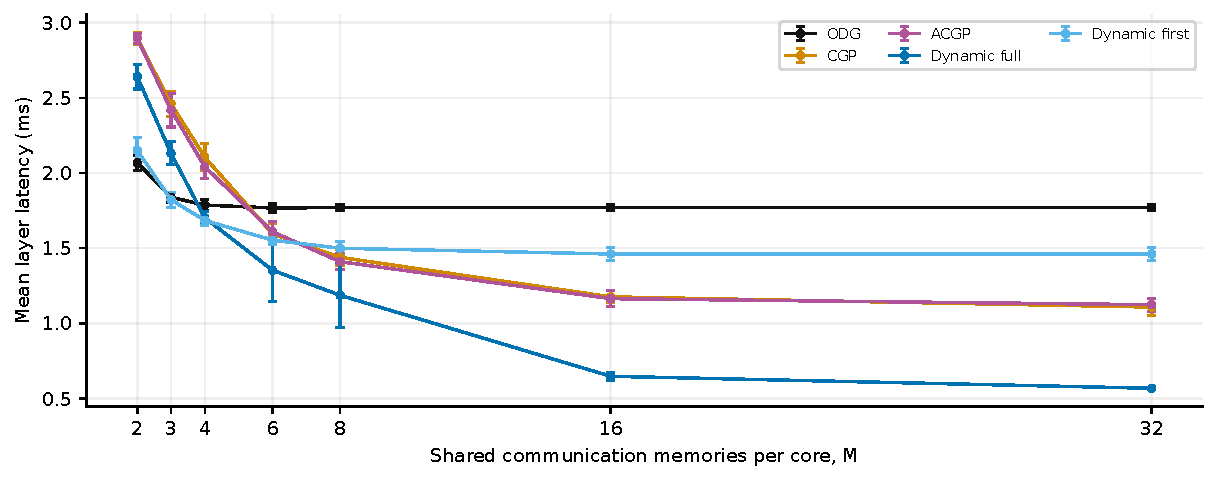
\includegraphics[width=.94\linewidth,height=.255\textheight,keepaspectratio]{figures/memory/mesh_shortest_reliable_avg_layer_latency_ms.pdf}\captionof{figure}{Run-level mean and sample SD. Shared trace aliases are counted once.}\end{center}
\begin{center}{\scriptsize\setlength{\tabcolsep}{3pt}
\begin{tabular}{lrrrrr}
\toprule
M & ODG & CGP & ACGP & Dynamic full & Dynamic first \\
\midrule
2 & $2.069\pm0.050$ & $2.896\pm0.040$ & $2.897\pm0.032$ & $2.641\pm0.082$ & $2.150\pm0.084$ \\
3 & $1.838\pm0.034$ & $2.460\pm0.085$ & $2.419\pm0.112$ & $2.131\pm0.077$ & $1.822\pm0.051$ \\
4 & $1.787\pm0.038$ & $2.105\pm0.091$ & $2.041\pm0.078$ & $1.702\pm0.040$ & $1.684\pm0.034$ \\
6 & $1.767\pm0.028$ & $1.595\pm0.068$ & $1.609\pm0.070$ & $1.353\pm0.211$ & $1.553\pm0.031$ \\
8 & $1.770\pm0.022$ & $1.439\pm0.051$ & $1.410\pm0.053$ & $1.186\pm0.215$ & $1.499\pm0.045$ \\
16 & $1.770\pm0.022$ & $1.176\pm0.039$ & $1.164\pm0.051$ & $0.6470\pm0.0254$ & $1.461\pm0.046$ \\
32 & $1.770\pm0.022$ & $1.108\pm0.056$ & $1.123\pm0.043$ & $0.5671\pm0.0031$ & $1.461\pm0.046$ \\
\bottomrule\end{tabular}}
\captionof{table}{Mean $\pm$ sample SD; n/a denotes a metric outside that policy's instrumentation.}
{\footnotesize\href{https://github.com/sanjeevkrishnaa/Compiler-Driven-ACE/blob/codex/ace-scheduler-correctness/docs/latex/qft96_final/data/memory_mesh_shortest_reliable_avg_layer_latency_ms.csv}{Exact CSV values and sample counts}}
\end{center}
\subsection*{Maximum layer latency}
\begin{center}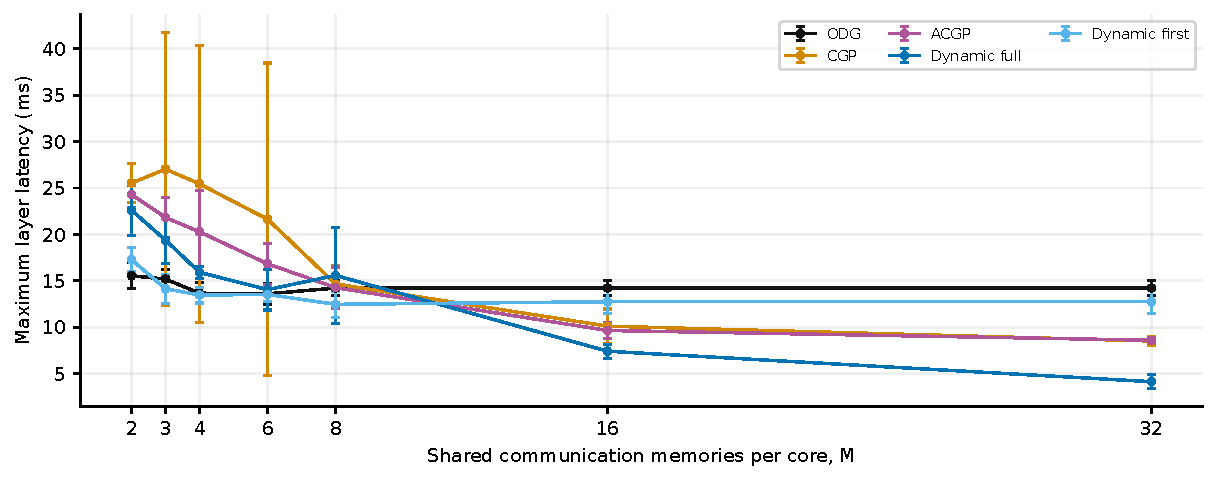
\includegraphics[width=.94\linewidth,height=.255\textheight,keepaspectratio]{figures/memory/mesh_shortest_reliable_max_layer_latency_ms.pdf}\captionof{figure}{Run-level mean and sample SD. Shared trace aliases are counted once.}\end{center}
\begin{center}{\scriptsize\setlength{\tabcolsep}{3pt}
\begin{tabular}{lrrrrr}
\toprule
M & ODG & CGP & ACGP & Dynamic full & Dynamic first \\
\midrule
2 & $15.550\pm1.408$ & $25.527\pm2.109$ & $24.296\pm1.387$ & $22.601\pm2.685$ & $17.267\pm1.320$ \\
3 & $15.184\pm1.042$ & $27.034\pm14.738$ & $21.817\pm2.120$ & $19.384\pm2.499$ & $14.150\pm1.559$ \\
4 & $13.667\pm1.159$ & $25.444\pm14.897$ & $20.276\pm4.452$ & $15.917\pm0.627$ & $13.467\pm0.855$ \\
6 & $13.600\pm1.108$ & $21.640\pm16.826$ & $16.834\pm2.204$ & $14.050\pm2.197$ & $13.534\pm0.747$ \\
8 & $14.217\pm0.842$ & $14.664\pm2.007$ & $14.266\pm2.220$ & $15.584\pm5.209$ & $12.467\pm1.435$ \\
16 & $14.217\pm0.842$ & $10.117\pm1.850$ & $9.650\pm0.874$ & $7.417\pm0.757$ & $12.750\pm1.294$ \\
32 & $14.217\pm0.842$ & $8.517\pm0.467$ & $8.600\pm0.310$ & $4.133\pm0.761$ & $12.750\pm1.294$ \\
\bottomrule\end{tabular}}
\captionof{table}{Mean $\pm$ sample SD; n/a denotes a metric outside that policy's instrumentation.}
{\footnotesize\href{https://github.com/sanjeevkrishnaa/Compiler-Driven-ACE/blob/codex/ace-scheduler-correctness/docs/latex/qft96_final/data/memory_mesh_shortest_reliable_max_layer_latency_ms.csv}{Exact CSV values and sample counts}}
\end{center}
\clearpage
\subsection*{Minimum layer latency}
\begin{center}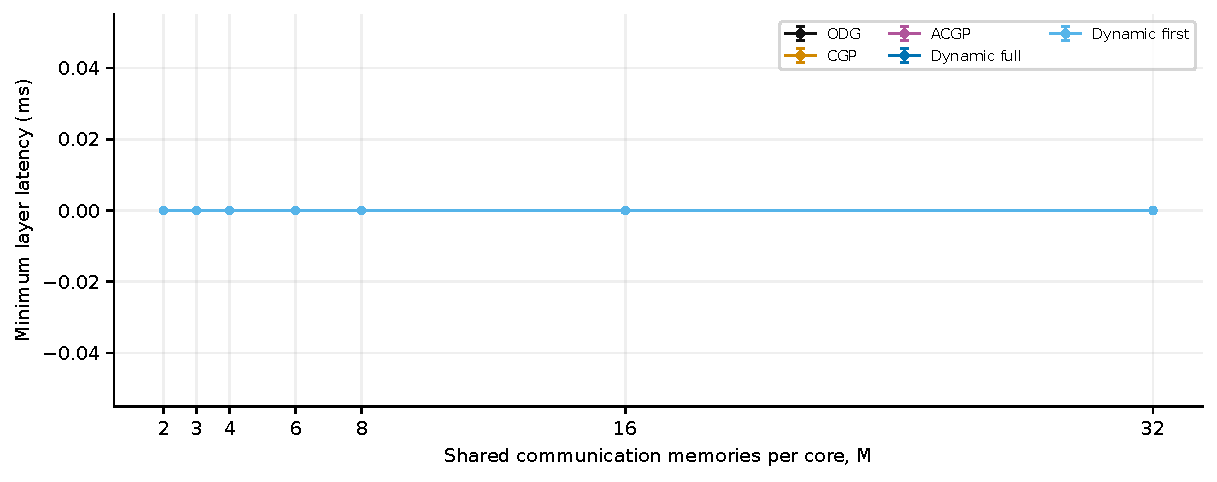
\includegraphics[width=.94\linewidth,height=.255\textheight,keepaspectratio]{figures/memory/mesh_shortest_reliable_min_layer_latency_ms.pdf}\captionof{figure}{Run-level mean and sample SD. Shared trace aliases are counted once.}\end{center}
\begin{center}{\scriptsize\setlength{\tabcolsep}{3pt}
\begin{tabular}{lrrrrr}
\toprule
M & ODG & CGP & ACGP & Dynamic full & Dynamic first \\
\midrule
2 & $0.0000\pm0.0000$ & $0.0000\pm0.0000$ & $0.0000\pm0.0000$ & $0.0000\pm0.0000$ & $0.0000\pm0.0000$ \\
3 & $0.0000\pm0.0000$ & $0.0000\pm0.0000$ & $0.0000\pm0.0000$ & $0.0000\pm0.0000$ & $0.0000\pm0.0000$ \\
4 & $0.0000\pm0.0000$ & $0.0000\pm0.0000$ & $0.0000\pm0.0000$ & $0.0000\pm0.0000$ & $0.0000\pm0.0000$ \\
6 & $0.0000\pm0.0000$ & $0.0000\pm0.0000$ & $0.0000\pm0.0000$ & $0.0000\pm0.0000$ & $0.0000\pm0.0000$ \\
8 & $0.0000\pm0.0000$ & $0.0000\pm0.0000$ & $0.0000\pm0.0000$ & $0.0000\pm0.0000$ & $0.0000\pm0.0000$ \\
16 & $0.0000\pm0.0000$ & $0.0000\pm0.0000$ & $0.0000\pm0.0000$ & $0.0000\pm0.0000$ & $0.0000\pm0.0000$ \\
32 & $0.0000\pm0.0000$ & $0.0000\pm0.0000$ & $0.0000\pm0.0000$ & $0.0000\pm0.0000$ & $0.0000\pm0.0000$ \\
\bottomrule\end{tabular}}
\captionof{table}{Mean $\pm$ sample SD; n/a denotes a metric outside that policy's instrumentation.}
{\footnotesize\href{https://github.com/sanjeevkrishnaa/Compiler-Driven-ACE/blob/codex/ace-scheduler-correctness/docs/latex/qft96_final/data/memory_mesh_shortest_reliable_min_layer_latency_ms.csv}{Exact CSV values and sample counts}}
\end{center}
\section{Max Reliability}
\clearpage
\subsection*{Mean request latency}
\begin{center}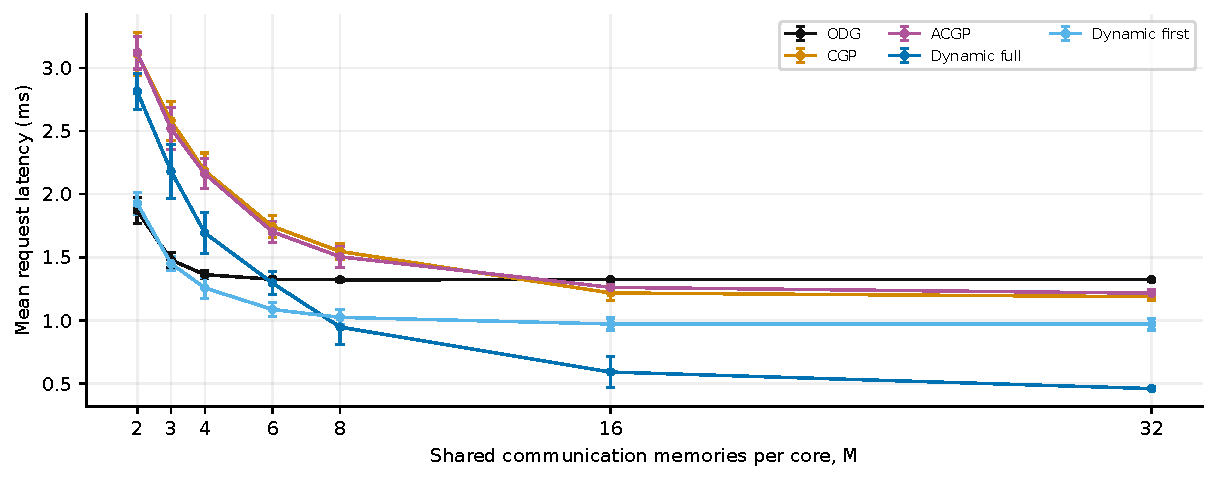
\includegraphics[width=.94\linewidth,height=.255\textheight,keepaspectratio]{figures/memory/mesh_max_reliability_request_latency_mean_ms.pdf}\captionof{figure}{Run-level mean and sample SD. Shared trace aliases are counted once.}\end{center}
\begin{center}{\scriptsize\setlength{\tabcolsep}{3pt}
\begin{tabular}{lrrrrr}
\toprule
M & ODG & CGP & ACGP & Dynamic full & Dynamic first \\
\midrule
2 & $1.871\pm0.106$ & $3.111\pm0.170$ & $3.120\pm0.130$ & $2.813\pm0.145$ & $1.926\pm0.084$ \\
3 & $1.479\pm0.057$ & $2.580\pm0.153$ & $2.519\pm0.165$ & $2.182\pm0.213$ & $1.450\pm0.056$ \\
4 & $1.362\pm0.032$ & $2.183\pm0.142$ & $2.162\pm0.120$ & $1.693\pm0.164$ & $1.257\pm0.083$ \\
6 & $1.326\pm0.014$ & $1.745\pm0.088$ & $1.701\pm0.085$ & $1.296\pm0.090$ & $1.086\pm0.056$ \\
8 & $1.322\pm0.011$ & $1.546\pm0.066$ & $1.504\pm0.085$ & $0.9469\pm0.1370$ & $1.024\pm0.061$ \\
16 & $1.322\pm0.012$ & $1.217\pm0.061$ & $1.262\pm0.042$ & $0.5912\pm0.1245$ & $0.9715\pm0.0476$ \\
32 & $1.322\pm0.012$ & $1.188\pm0.027$ & $1.215\pm0.029$ & $0.4599\pm0.0011$ & $0.9706\pm0.0465$ \\
\bottomrule\end{tabular}}
\captionof{table}{Mean $\pm$ sample SD; n/a denotes a metric outside that policy's instrumentation.}
{\footnotesize\href{https://github.com/sanjeevkrishnaa/Compiler-Driven-ACE/blob/codex/ace-scheduler-correctness/docs/latex/qft96_final/data/memory_mesh_max_reliability_request_latency_mean_ms.csv}{Exact CSV values and sample counts}}
\end{center}
\subsection*{Median request latency}
\begin{center}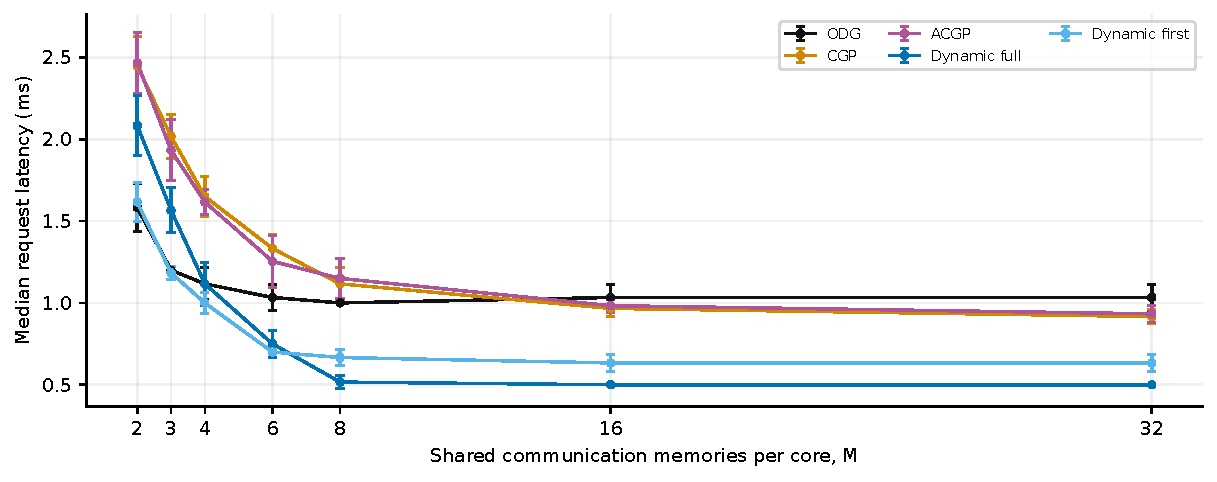
\includegraphics[width=.94\linewidth,height=.255\textheight,keepaspectratio]{figures/memory/mesh_max_reliability_request_latency_median_ms.pdf}\captionof{figure}{Run-level mean and sample SD. Shared trace aliases are counted once.}\end{center}
\begin{center}{\scriptsize\setlength{\tabcolsep}{3pt}
\begin{tabular}{lrrrrr}
\toprule
M & ODG & CGP & ACGP & Dynamic full & Dynamic first \\
\midrule
2 & $1.583\pm0.147$ & $2.450\pm0.176$ & $2.467\pm0.186$ & $2.083\pm0.183$ & $1.617\pm0.117$ \\
3 & $1.200\pm0.000$ & $2.017\pm0.133$ & $1.933\pm0.186$ & $1.567\pm0.137$ & $1.183\pm0.041$ \\
4 & $1.117\pm0.098$ & $1.650\pm0.122$ & $1.617\pm0.075$ & $1.117\pm0.133$ & $1.000\pm0.063$ \\
6 & $1.033\pm0.082$ & $1.333\pm0.082$ & $1.254\pm0.157$ & $0.7500\pm0.0837$ & $0.7000\pm0.0000$ \\
8 & $1.000\pm0.000$ & $1.117\pm0.098$ & $1.150\pm0.122$ & $0.5167\pm0.0408$ & $0.6667\pm0.0516$ \\
16 & $1.033\pm0.082$ & $0.9667\pm0.0516$ & $0.9833\pm0.0408$ & $0.5000\pm0.0000$ & $0.6333\pm0.0516$ \\
32 & $1.033\pm0.082$ & $0.9167\pm0.0408$ & $0.9333\pm0.0516$ & $0.5000\pm0.0000$ & $0.6333\pm0.0516$ \\
\bottomrule\end{tabular}}
\captionof{table}{Mean $\pm$ sample SD; n/a denotes a metric outside that policy's instrumentation.}
{\footnotesize\href{https://github.com/sanjeevkrishnaa/Compiler-Driven-ACE/blob/codex/ace-scheduler-correctness/docs/latex/qft96_final/data/memory_mesh_max_reliability_request_latency_median_ms.csv}{Exact CSV values and sample counts}}
\end{center}
\clearpage
\subsection*{p95 request latency}
\begin{center}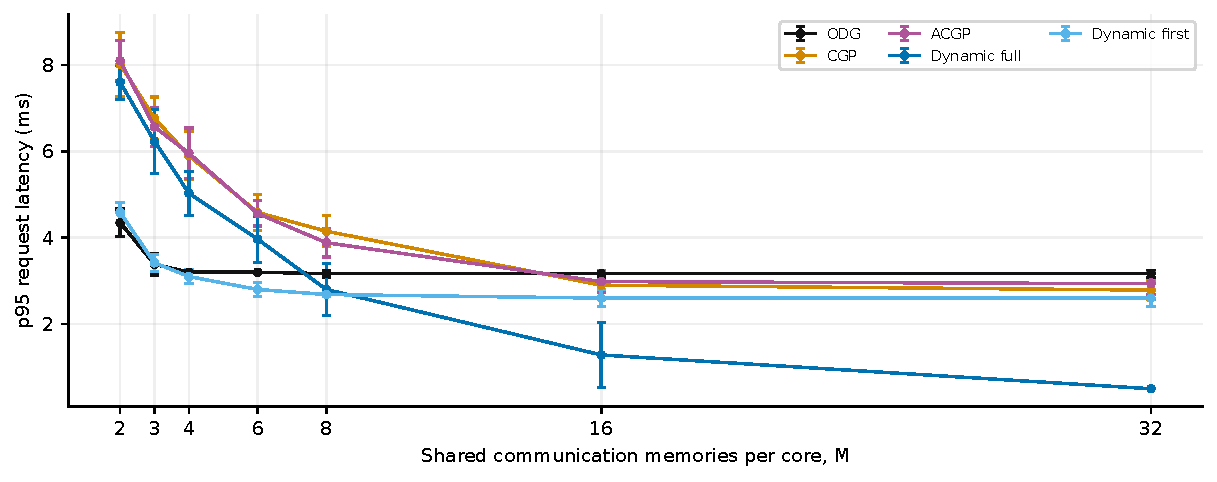
\includegraphics[width=.94\linewidth,height=.255\textheight,keepaspectratio]{figures/memory/mesh_max_reliability_request_latency_p95_ms.pdf}\captionof{figure}{Run-level mean and sample SD. Shared trace aliases are counted once.}\end{center}
\begin{center}{\scriptsize\setlength{\tabcolsep}{3pt}
\begin{tabular}{lrrrrr}
\toprule
M & ODG & CGP & ACGP & Dynamic full & Dynamic first \\
\midrule
2 & $4.350\pm0.315$ & $8.017\pm0.741$ & $8.100\pm0.465$ & $7.600\pm0.395$ & $4.583\pm0.240$ \\
3 & $3.383\pm0.248$ & $6.767\pm0.493$ & $6.567\pm0.446$ & $6.233\pm0.742$ & $3.417\pm0.194$ \\
4 & $3.200\pm0.000$ & $5.900\pm0.551$ & $5.956\pm0.585$ & $5.033\pm0.509$ & $3.100\pm0.155$ \\
6 & $3.200\pm0.000$ & $4.584\pm0.407$ & $4.562\pm0.291$ & $3.967\pm0.532$ & $2.800\pm0.155$ \\
8 & $3.167\pm0.082$ & $4.150\pm0.362$ & $3.883\pm0.331$ & $2.800\pm0.593$ & $2.683\pm0.041$ \\
16 & $3.167\pm0.082$ & $2.900\pm0.322$ & $2.983\pm0.256$ & $1.283\pm0.744$ & $2.600\pm0.200$ \\
32 & $3.167\pm0.082$ & $2.785\pm0.223$ & $2.933\pm0.250$ & $0.5000\pm0.0000$ & $2.600\pm0.200$ \\
\bottomrule\end{tabular}}
\captionof{table}{Mean $\pm$ sample SD; n/a denotes a metric outside that policy's instrumentation.}
{\footnotesize\href{https://github.com/sanjeevkrishnaa/Compiler-Driven-ACE/blob/codex/ace-scheduler-correctness/docs/latex/qft96_final/data/memory_mesh_max_reliability_request_latency_p95_ms.csv}{Exact CSV values and sample counts}}
\end{center}
\subsection*{Maximum request latency}
\begin{center}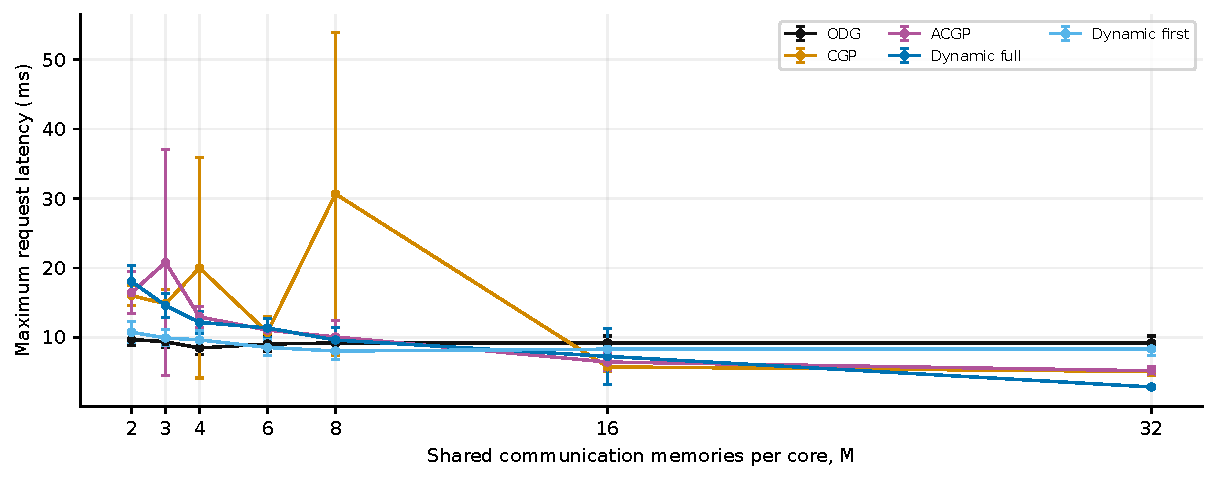
\includegraphics[width=.94\linewidth,height=.255\textheight,keepaspectratio]{figures/memory/mesh_max_reliability_request_latency_max_ms.pdf}\captionof{figure}{Run-level mean and sample SD. Shared trace aliases are counted once.}\end{center}
\begin{center}{\scriptsize\setlength{\tabcolsep}{3pt}
\begin{tabular}{lrrrrr}
\toprule
M & ODG & CGP & ACGP & Dynamic full & Dynamic first \\
\midrule
2 & $9.700\pm0.795$ & $16.011\pm1.439$ & $16.417\pm3.024$ & $18.067\pm2.242$ & $10.750\pm1.537$ \\
3 & $9.367\pm0.774$ & $14.845\pm2.030$ & $20.793\pm16.325$ & $14.584\pm1.699$ & $9.917\pm1.155$ \\
4 & $8.467\pm0.973$ & $19.999\pm15.855$ & $12.950\pm1.549$ & $12.167\pm1.598$ & $9.634\pm1.322$ \\
6 & $9.034\pm1.033$ & $10.734\pm2.270$ & $11.049\pm1.642$ & $11.350\pm1.358$ & $8.550\pm1.164$ \\
8 & $9.200\pm1.000$ & $30.659\pm23.276$ & $10.061\pm2.307$ & $9.617\pm1.777$ & $8.034\pm1.211$ \\
16 & $9.200\pm1.000$ & $5.752\pm0.612$ & $6.450\pm1.154$ & $7.267\pm4.016$ & $8.300\pm0.959$ \\
32 & $9.200\pm1.000$ & $5.083\pm0.546$ & $5.183\pm0.564$ & $2.850\pm0.251$ & $8.317\pm0.947$ \\
\bottomrule\end{tabular}}
\captionof{table}{Mean $\pm$ sample SD; n/a denotes a metric outside that policy's instrumentation.}
{\footnotesize\href{https://github.com/sanjeevkrishnaa/Compiler-Driven-ACE/blob/codex/ace-scheduler-correctness/docs/latex/qft96_final/data/memory_mesh_max_reliability_request_latency_max_ms.csv}{Exact CSV values and sample counts}}
\end{center}
\clearpage
\subsection*{Communication makespan}
\begin{center}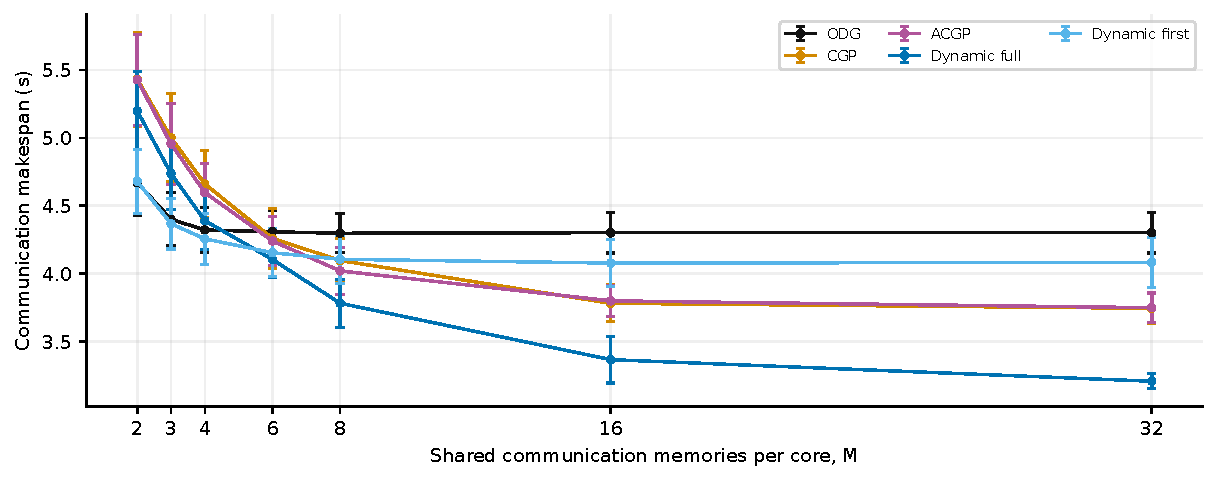
\includegraphics[width=.94\linewidth,height=.255\textheight,keepaspectratio]{figures/memory/mesh_max_reliability_end_to_end_latency_ms.pdf}\captionof{figure}{Run-level mean and sample SD. Shared trace aliases are counted once.}\end{center}
\begin{center}{\scriptsize\setlength{\tabcolsep}{3pt}
\begin{tabular}{lrrrrr}
\toprule
M & ODG & CGP & ACGP & Dynamic full & Dynamic first \\
\midrule
2 & $4.670\pm0.244$ & $5.434\pm0.345$ & $5.429\pm0.336$ & $5.201\pm0.288$ & $4.681\pm0.237$ \\
3 & $4.401\pm0.195$ & $5.002\pm0.323$ & $4.956\pm0.301$ & $4.737\pm0.266$ & $4.367\pm0.186$ \\
4 & $4.321\pm0.164$ & $4.661\pm0.244$ & $4.598\pm0.214$ & $4.390\pm0.214$ & $4.256\pm0.188$ \\
6 & $4.308\pm0.157$ & $4.260\pm0.220$ & $4.240\pm0.183$ & $4.104\pm0.132$ & $4.154\pm0.177$ \\
8 & $4.297\pm0.144$ & $4.096\pm0.165$ & $4.020\pm0.174$ & $3.781\pm0.178$ & $4.106\pm0.175$ \\
16 & $4.302\pm0.150$ & $3.781\pm0.135$ & $3.799\pm0.117$ & $3.365\pm0.172$ & $4.077\pm0.174$ \\
32 & $4.302\pm0.150$ & $3.744\pm0.114$ & $3.748\pm0.109$ & $3.206\pm0.055$ & $4.083\pm0.182$ \\
\bottomrule\end{tabular}}
\captionof{table}{Mean $\pm$ sample SD; n/a denotes a metric outside that policy's instrumentation.}
{\footnotesize\href{https://github.com/sanjeevkrishnaa/Compiler-Driven-ACE/blob/codex/ace-scheduler-correctness/docs/latex/qft96_final/data/memory_mesh_max_reliability_end_to_end_latency_ms.csv}{Exact CSV values and sample counts}}
\end{center}
\subsection*{Mean admission wait}
\begin{center}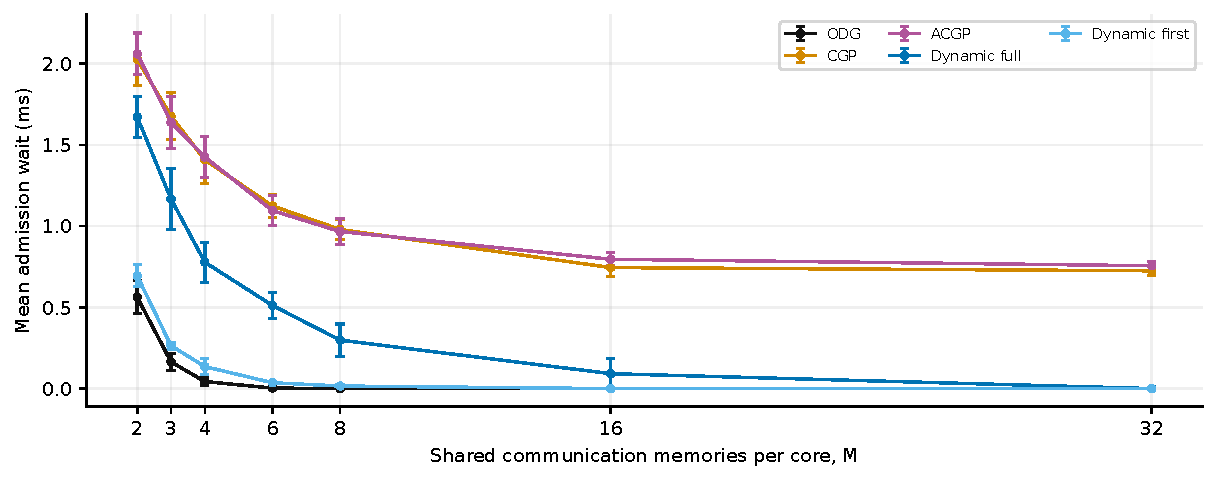
\includegraphics[width=.94\linewidth,height=.255\textheight,keepaspectratio]{figures/memory/mesh_max_reliability_average_admission_wait_ms.pdf}\captionof{figure}{Run-level mean and sample SD. Shared trace aliases are counted once.}\end{center}
\begin{center}{\scriptsize\setlength{\tabcolsep}{3pt}
\begin{tabular}{lrrrrr}
\toprule
M & ODG & CGP & ACGP & Dynamic full & Dynamic first \\
\midrule
2 & $0.5628\pm0.1018$ & $2.028\pm0.165$ & $2.060\pm0.129$ & $1.671\pm0.127$ & $0.6942\pm0.0683$ \\
3 & $0.1644\pm0.0510$ & $1.677\pm0.144$ & $1.639\pm0.161$ & $1.167\pm0.189$ & $0.2639\pm0.0227$ \\
4 & $0.0435\pm0.0225$ & $1.408\pm0.144$ & $1.426\pm0.129$ & $0.7779\pm0.1230$ & $0.1357\pm0.0479$ \\
6 & $0.0033\pm0.0041$ & $1.124\pm0.070$ & $1.095\pm0.092$ & $0.5119\pm0.0809$ & $0.0361\pm0.0031$ \\
8 & $0.0001\pm0.0002$ & $0.9793\pm0.0615$ & $0.9670\pm0.0816$ & $0.2984\pm0.0995$ & $0.0161\pm0.0108$ \\
16 & $0.0000\pm0.0000$ & $0.7450\pm0.0555$ & $0.7962\pm0.0387$ & $0.0921\pm0.0910$ & $0.0000\pm0.0000$ \\
32 & $0.0000\pm0.0000$ & $0.7251\pm0.0290$ & $0.7561\pm0.0267$ & $0.0001\pm0.0002$ & $0.0000\pm0.0000$ \\
\bottomrule\end{tabular}}
\captionof{table}{Mean $\pm$ sample SD; n/a denotes a metric outside that policy's instrumentation.}
{\footnotesize\href{https://github.com/sanjeevkrishnaa/Compiler-Driven-ACE/blob/codex/ace-scheduler-correctness/docs/latex/qft96_final/data/memory_mesh_max_reliability_average_admission_wait_ms.csv}{Exact CSV values and sample counts}}
\end{center}
\clearpage
\subsection*{Delivered EPR fidelity}
\begin{center}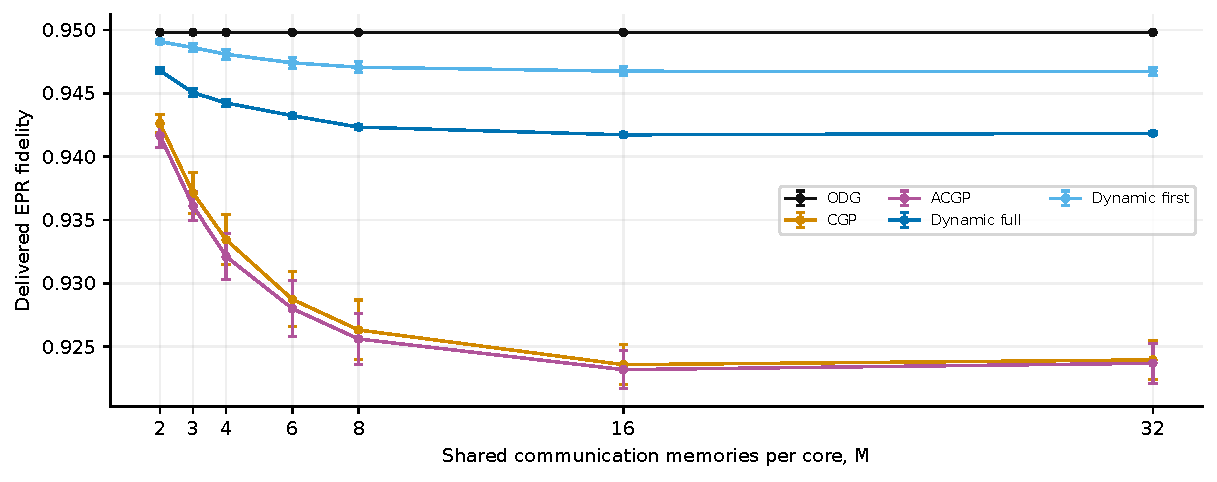
\includegraphics[width=.94\linewidth,height=.255\textheight,keepaspectratio]{figures/memory/mesh_max_reliability_average_delivered_epr_fidelity.pdf}\captionof{figure}{Run-level mean and sample SD. Shared trace aliases are counted once.}\end{center}
\begin{center}{\scriptsize\setlength{\tabcolsep}{3pt}
\begin{tabular}{lrrrrr}
\toprule
M & ODG & CGP & ACGP & Dynamic full & Dynamic first \\
\midrule
2 & $0.9498\pm0.0000$ & $0.9426\pm0.0007$ & $0.9417\pm0.0009$ & $0.9468\pm0.0002$ & $0.9491\pm0.0002$ \\
3 & $0.9498\pm0.0000$ & $0.9371\pm0.0016$ & $0.9361\pm0.0012$ & $0.9451\pm0.0003$ & $0.9486\pm0.0003$ \\
4 & $0.9498\pm0.0000$ & $0.9334\pm0.0020$ & $0.9321\pm0.0018$ & $0.9442\pm0.0002$ & $0.9481\pm0.0004$ \\
6 & $0.9498\pm0.0000$ & $0.9287\pm0.0022$ & $0.9280\pm0.0022$ & $0.9432\pm0.0002$ & $0.9474\pm0.0004$ \\
8 & $0.9498\pm0.0000$ & $0.9263\pm0.0024$ & $0.9256\pm0.0020$ & $0.9423\pm0.0002$ & $0.9471\pm0.0004$ \\
16 & $0.9498\pm0.0000$ & $0.9236\pm0.0016$ & $0.9232\pm0.0015$ & $0.9417\pm0.0002$ & $0.9467\pm0.0004$ \\
32 & $0.9498\pm0.0000$ & $0.9240\pm0.0015$ & $0.9237\pm0.0016$ & $0.9418\pm0.0001$ & $0.9467\pm0.0003$ \\
\bottomrule\end{tabular}}
\captionof{table}{Mean $\pm$ sample SD; n/a denotes a metric outside that policy's instrumentation.}
{\footnotesize\href{https://github.com/sanjeevkrishnaa/Compiler-Driven-ACE/blob/codex/ace-scheduler-correctness/docs/latex/qft96_final/data/memory_mesh_max_reliability_average_delivered_epr_fidelity.csv}{Exact CSV values and sample counts}}
\end{center}
\subsection*{Compiler readiness fraction}
\begin{center}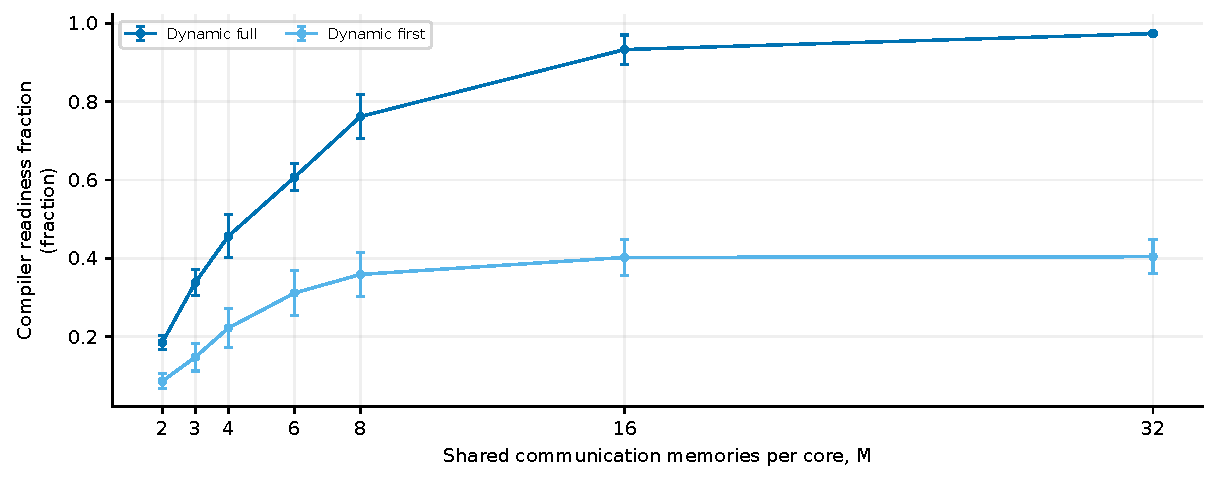
\includegraphics[width=.94\linewidth,height=.255\textheight,keepaspectratio]{figures/memory/mesh_max_reliability_pregenerated_success_rate.pdf}\captionof{figure}{Run-level mean and sample SD. Shared trace aliases are counted once.}\end{center}
\begin{center}{\scriptsize\setlength{\tabcolsep}{3pt}
\begin{tabular}{lrrrrr}
\toprule
M & ODG & CGP & ACGP & Dynamic full & Dynamic first \\
\midrule
2 & n/a & n/a & n/a & $0.1851\pm0.0189$ & $0.0860\pm0.0191$ \\
3 & n/a & n/a & n/a & $0.3381\pm0.0332$ & $0.1475\pm0.0353$ \\
4 & n/a & n/a & n/a & $0.4564\pm0.0549$ & $0.2219\pm0.0499$ \\
6 & n/a & n/a & n/a & $0.6067\pm0.0344$ & $0.3113\pm0.0575$ \\
8 & n/a & n/a & n/a & $0.7621\pm0.0552$ & $0.3588\pm0.0561$ \\
16 & n/a & n/a & n/a & $0.9331\pm0.0371$ & $0.4024\pm0.0452$ \\
32 & n/a & n/a & n/a & $0.9739\pm0.0032$ & $0.4041\pm0.0429$ \\
\bottomrule\end{tabular}}
\captionof{table}{Mean $\pm$ sample SD; n/a denotes a metric outside that policy's instrumentation.}
{\footnotesize\href{https://github.com/sanjeevkrishnaa/Compiler-Driven-ACE/blob/codex/ace-scheduler-correctness/docs/latex/qft96_final/data/memory_mesh_max_reliability_pregenerated_success_rate.csv}{Exact CSV values and sample counts}}
\end{center}
\clearpage
\subsection*{Intended compiler-hit fraction}
\begin{center}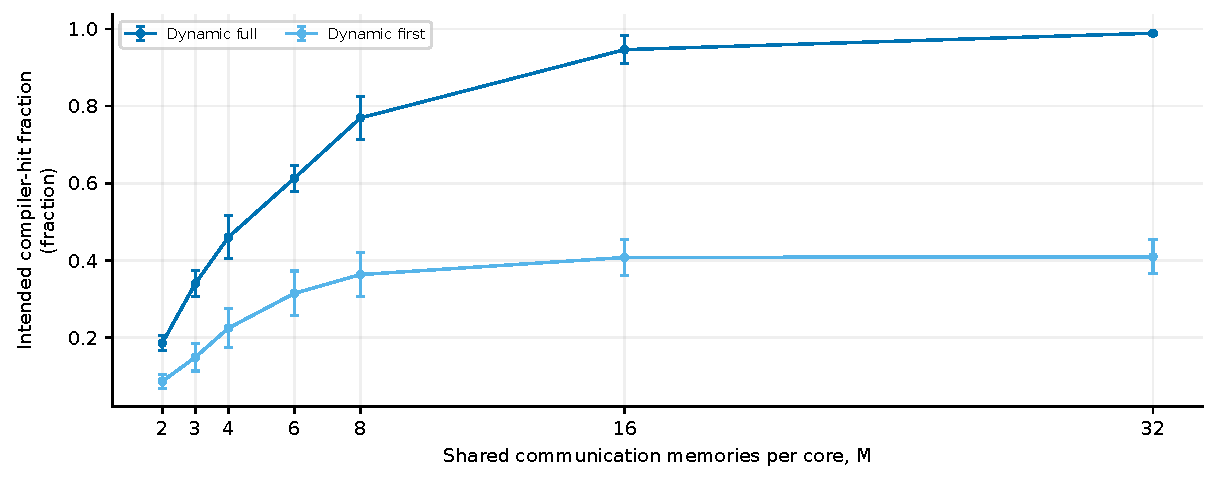
\includegraphics[width=.94\linewidth,height=.255\textheight,keepaspectratio]{figures/memory/mesh_max_reliability_intended_request_hit_rate.pdf}\captionof{figure}{Run-level mean and sample SD. Shared trace aliases are counted once.}\end{center}
\begin{center}{\scriptsize\setlength{\tabcolsep}{3pt}
\begin{tabular}{lrrrrr}
\toprule
M & ODG & CGP & ACGP & Dynamic full & Dynamic first \\
\midrule
2 & n/a & n/a & n/a & $0.1860\pm0.0187$ & $0.0868\pm0.0190$ \\
3 & n/a & n/a & n/a & $0.3402\pm0.0331$ & $0.1491\pm0.0354$ \\
4 & n/a & n/a & n/a & $0.4600\pm0.0554$ & $0.2246\pm0.0509$ \\
6 & n/a & n/a & n/a & $0.6131\pm0.0337$ & $0.3149\pm0.0579$ \\
8 & n/a & n/a & n/a & $0.7693\pm0.0550$ & $0.3634\pm0.0571$ \\
16 & n/a & n/a & n/a & $0.9461\pm0.0363$ & $0.4078\pm0.0461$ \\
32 & n/a & n/a & n/a & $0.9887\pm0.0022$ & $0.4096\pm0.0437$ \\
\bottomrule\end{tabular}}
\captionof{table}{Mean $\pm$ sample SD; n/a denotes a metric outside that policy's instrumentation.}
{\footnotesize\href{https://github.com/sanjeevkrishnaa/Compiler-Driven-ACE/blob/codex/ace-scheduler-correctness/docs/latex/qft96_final/data/memory_mesh_max_reliability_intended_request_hit_rate.csv}{Exact CSV values and sample counts}}
\end{center}
\subsection*{Compiler fallback fraction}
\begin{center}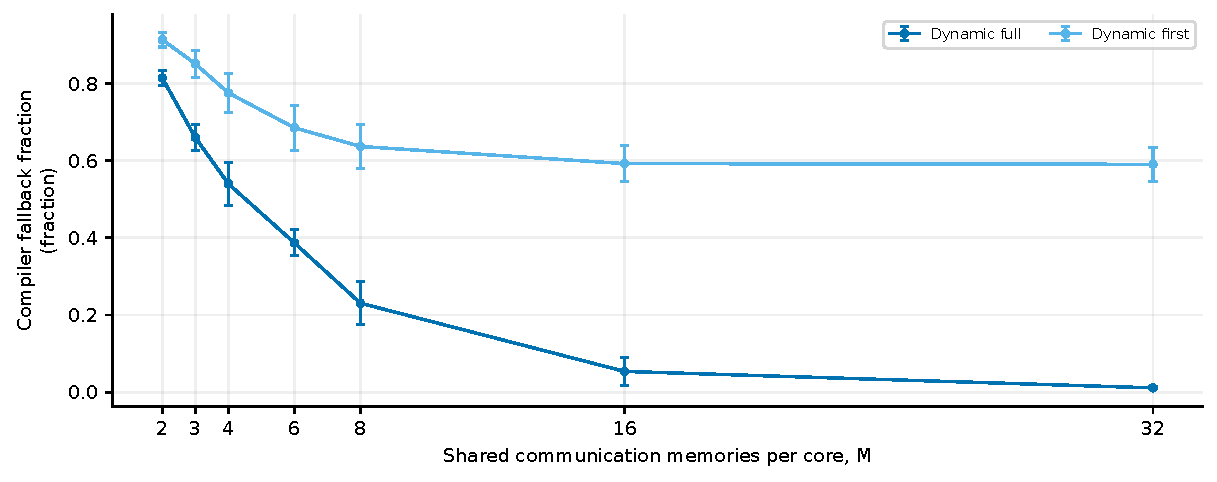
\includegraphics[width=.94\linewidth,height=.255\textheight,keepaspectratio]{figures/memory/mesh_max_reliability_on_demand_fallback_rate.pdf}\captionof{figure}{Run-level mean and sample SD. Shared trace aliases are counted once.}\end{center}
\begin{center}{\scriptsize\setlength{\tabcolsep}{3pt}
\begin{tabular}{lrrrrr}
\toprule
M & ODG & CGP & ACGP & Dynamic full & Dynamic first \\
\midrule
2 & n/a & n/a & n/a & $0.8140\pm0.0187$ & $0.9132\pm0.0190$ \\
3 & n/a & n/a & n/a & $0.6598\pm0.0331$ & $0.8509\pm0.0354$ \\
4 & n/a & n/a & n/a & $0.5400\pm0.0554$ & $0.7754\pm0.0509$ \\
6 & n/a & n/a & n/a & $0.3869\pm0.0337$ & $0.6851\pm0.0579$ \\
8 & n/a & n/a & n/a & $0.2307\pm0.0550$ & $0.6366\pm0.0571$ \\
16 & n/a & n/a & n/a & $0.0539\pm0.0363$ & $0.5922\pm0.0461$ \\
32 & n/a & n/a & n/a & $0.0113\pm0.0022$ & $0.5904\pm0.0437$ \\
\bottomrule\end{tabular}}
\captionof{table}{Mean $\pm$ sample SD; n/a denotes a metric outside that policy's instrumentation.}
{\footnotesize\href{https://github.com/sanjeevkrishnaa/Compiler-Driven-ACE/blob/codex/ace-scheduler-correctness/docs/latex/qft96_final/data/memory_mesh_max_reliability_on_demand_fallback_rate.csv}{Exact CSV values and sample counts}}
\end{center}
\clearpage
\subsection*{Compiler-cache waste}
\begin{center}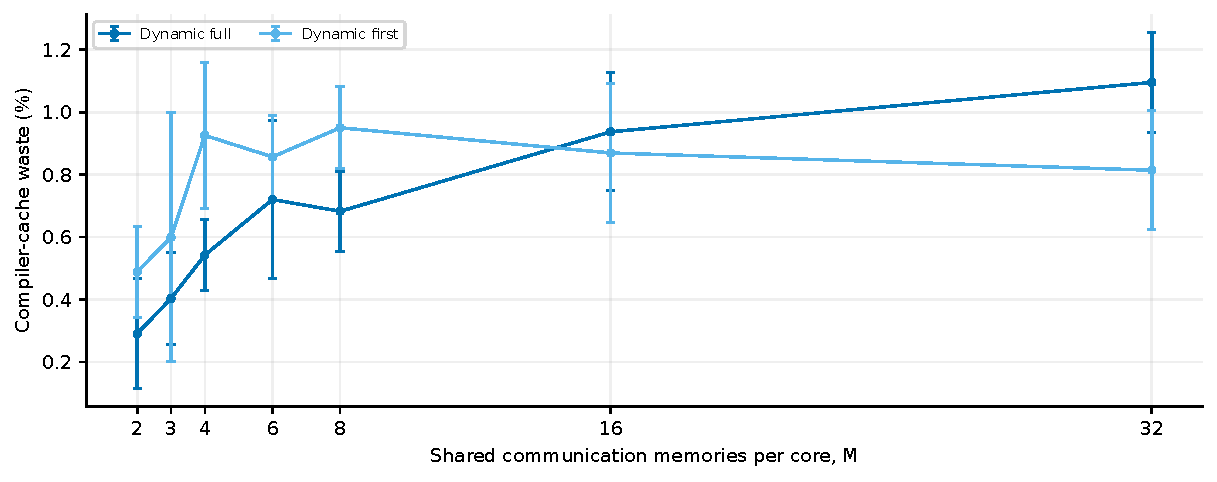
\includegraphics[width=.94\linewidth,height=.255\textheight,keepaspectratio]{figures/memory/mesh_max_reliability_compiler_waste_percentage.pdf}\captionof{figure}{Run-level mean and sample SD. Shared trace aliases are counted once.}\end{center}
\begin{center}{\scriptsize\setlength{\tabcolsep}{3pt}
\begin{tabular}{lrrrrr}
\toprule
M & ODG & CGP & ACGP & Dynamic full & Dynamic first \\
\midrule
2 & n/a & n/a & n/a & $0.2909\pm0.1762$ & $0.4889\pm0.1457$ \\
3 & n/a & n/a & n/a & $0.4037\pm0.1473$ & $0.5999\pm0.3993$ \\
4 & n/a & n/a & n/a & $0.5427\pm0.1146$ & $0.9258\pm0.2332$ \\
6 & n/a & n/a & n/a & $0.7204\pm0.2535$ & $0.8570\pm0.1323$ \\
8 & n/a & n/a & n/a & $0.6827\pm0.1275$ & $0.9503\pm0.1316$ \\
16 & n/a & n/a & n/a & $0.9372\pm0.1892$ & $0.8696\pm0.2216$ \\
32 & n/a & n/a & n/a & $1.095\pm0.160$ & $0.8142\pm0.1904$ \\
\bottomrule\end{tabular}}
\captionof{table}{Mean $\pm$ sample SD; n/a denotes a metric outside that policy's instrumentation.}
{\footnotesize\href{https://github.com/sanjeevkrishnaa/Compiler-Driven-ACE/blob/codex/ace-scheduler-correctness/docs/latex/qft96_final/data/memory_mesh_max_reliability_compiler_waste_percentage.csv}{Exact CSV values and sample counts}}
\end{center}
\subsection*{Native-protocol waste}
\begin{center}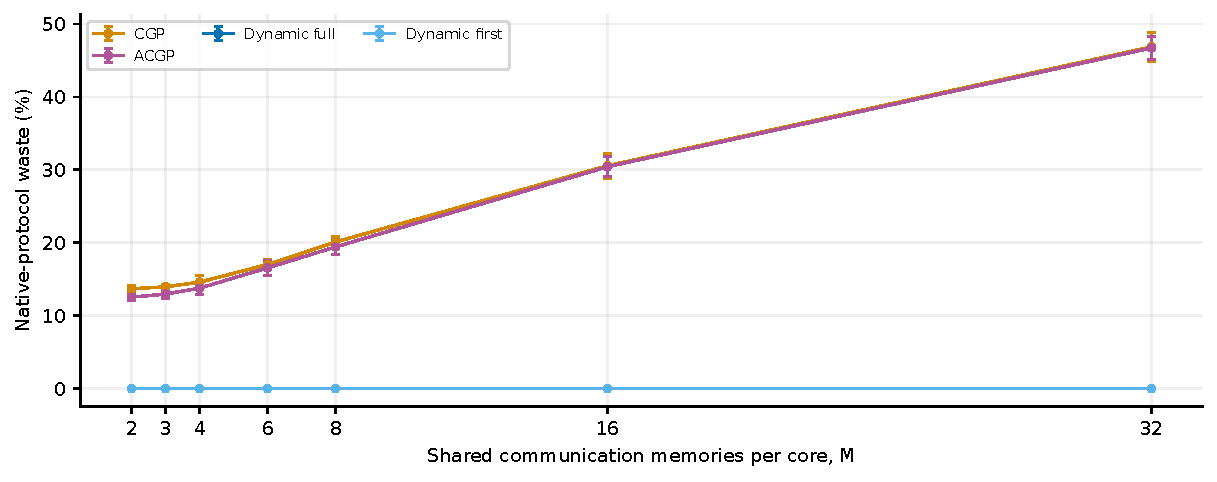
\includegraphics[width=.94\linewidth,height=.255\textheight,keepaspectratio]{figures/memory/mesh_max_reliability_protocol_waste_percentage.pdf}\captionof{figure}{Run-level mean and sample SD. Shared trace aliases are counted once.}\end{center}
\begin{center}{\scriptsize\setlength{\tabcolsep}{3pt}
\begin{tabular}{lrrrrr}
\toprule
M & ODG & CGP & ACGP & Dynamic full & Dynamic first \\
\midrule
2 & n/a & $13.698\pm0.495$ & $12.552\pm0.516$ & $0.0000\pm0.0000$ & $0.0000\pm0.0000$ \\
3 & n/a & $13.968\pm0.363$ & $12.973\pm0.624$ & $0.0000\pm0.0000$ & $0.0000\pm0.0000$ \\
4 & n/a & $14.604\pm0.896$ & $13.783\pm0.928$ & $0.0000\pm0.0000$ & $0.0000\pm0.0000$ \\
6 & n/a & $17.023\pm0.719$ & $16.565\pm1.026$ & $0.0000\pm0.0000$ & $0.0000\pm0.0000$ \\
8 & n/a & $20.113\pm0.761$ & $19.435\pm1.077$ & $0.0000\pm0.0000$ & $0.0000\pm0.0000$ \\
16 & n/a & $30.555\pm1.675$ & $30.424\pm1.394$ & $0.0000\pm0.0000$ & $0.0000\pm0.0000$ \\
32 & n/a & $46.848\pm1.994$ & $46.700\pm1.545$ & $0.0000\pm0.0000$ & $0.0000\pm0.0000$ \\
\bottomrule\end{tabular}}
\captionof{table}{Mean $\pm$ sample SD; n/a denotes a metric outside that policy's instrumentation.}
{\footnotesize\href{https://github.com/sanjeevkrishnaa/Compiler-Driven-ACE/blob/codex/ace-scheduler-correctness/docs/latex/qft96_final/data/memory_mesh_max_reliability_protocol_waste_percentage.csv}{Exact CSV values and sample counts}}
\end{center}
\clearpage
\subsection*{Compiler-pair expiry}
\begin{center}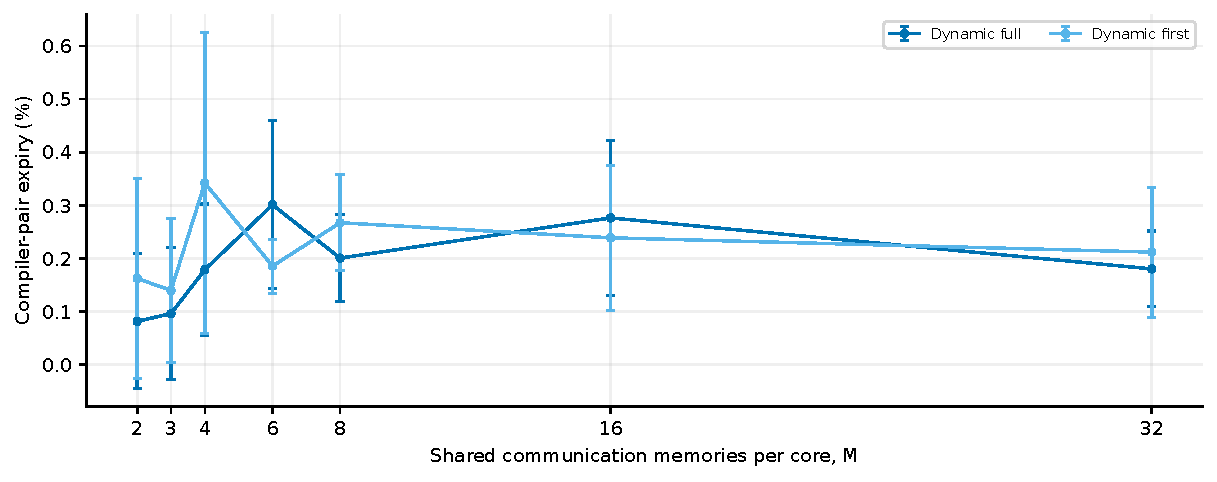
\includegraphics[width=.94\linewidth,height=.255\textheight,keepaspectratio]{figures/memory/mesh_max_reliability_compiler_expiry_percentage.pdf}\captionof{figure}{Run-level mean and sample SD. Shared trace aliases are counted once.}\end{center}
\begin{center}{\scriptsize\setlength{\tabcolsep}{3pt}
\begin{tabular}{lrrrrr}
\toprule
M & ODG & CGP & ACGP & Dynamic full & Dynamic first \\
\midrule
2 & n/a & n/a & n/a & $0.0818\pm0.1269$ & $0.1624\pm0.1878$ \\
3 & n/a & n/a & n/a & $0.0963\pm0.1242$ & $0.1400\pm0.1356$ \\
4 & n/a & n/a & n/a & $0.1790\pm0.1236$ & $0.3422\pm0.2835$ \\
6 & n/a & n/a & n/a & $0.3011\pm0.1580$ & $0.1857\pm0.0507$ \\
8 & n/a & n/a & n/a & $0.2008\pm0.0816$ & $0.2673\pm0.0904$ \\
16 & n/a & n/a & n/a & $0.2764\pm0.1461$ & $0.2390\pm0.1365$ \\
32 & n/a & n/a & n/a & $0.1804\pm0.0713$ & $0.2120\pm0.1222$ \\
\bottomrule\end{tabular}}
\captionof{table}{Mean $\pm$ sample SD; n/a denotes a metric outside that policy's instrumentation.}
{\footnotesize\href{https://github.com/sanjeevkrishnaa/Compiler-Driven-ACE/blob/codex/ace-scheduler-correctness/docs/latex/qft96_final/data/memory_mesh_max_reliability_compiler_expiry_percentage.csv}{Exact CSV values and sample counts}}
\end{center}
\subsection*{Used compiler-pair storage time}
\begin{center}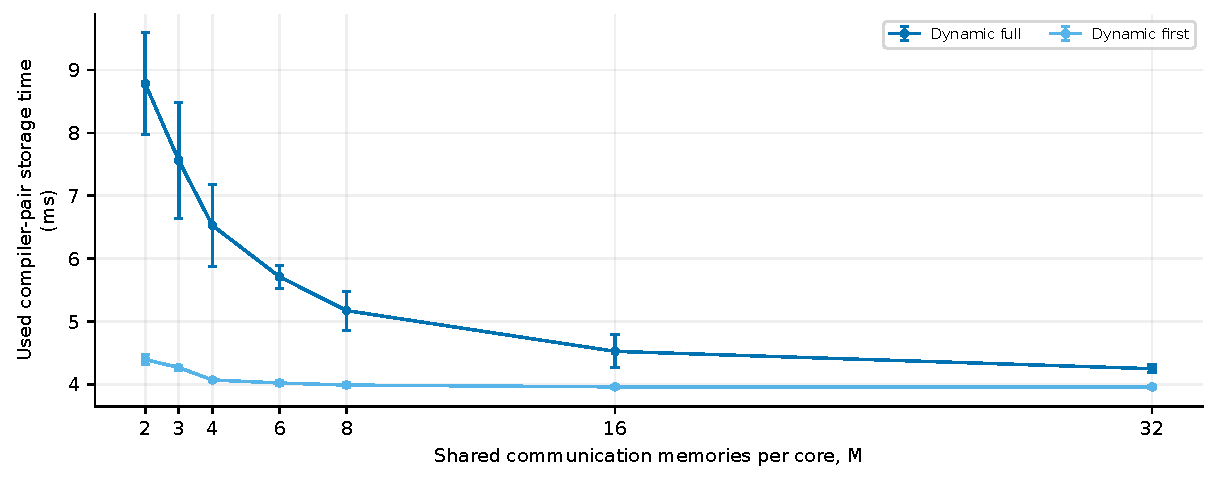
\includegraphics[width=.94\linewidth,height=.255\textheight,keepaspectratio]{figures/memory/mesh_max_reliability_average_storage_time_ms.pdf}\captionof{figure}{Run-level mean and sample SD. Shared trace aliases are counted once.}\end{center}
\begin{center}{\scriptsize\setlength{\tabcolsep}{3pt}
\begin{tabular}{lrrrrr}
\toprule
M & ODG & CGP & ACGP & Dynamic full & Dynamic first \\
\midrule
2 & n/a & n/a & n/a & $8.784\pm0.815$ & $4.394\pm0.084$ \\
3 & n/a & n/a & n/a & $7.562\pm0.925$ & $4.267\pm0.040$ \\
4 & n/a & n/a & n/a & $6.529\pm0.649$ & $4.070\pm0.019$ \\
6 & n/a & n/a & n/a & $5.711\pm0.184$ & $4.020\pm0.039$ \\
8 & n/a & n/a & n/a & $5.173\pm0.310$ & $3.988\pm0.041$ \\
16 & n/a & n/a & n/a & $4.524\pm0.261$ & $3.960\pm0.022$ \\
32 & n/a & n/a & n/a & $4.248\pm0.060$ & $3.958\pm0.028$ \\
\bottomrule\end{tabular}}
\captionof{table}{Mean $\pm$ sample SD; n/a denotes a metric outside that policy's instrumentation.}
{\footnotesize\href{https://github.com/sanjeevkrishnaa/Compiler-Driven-ACE/blob/codex/ace-scheduler-correctness/docs/latex/qft96_final/data/memory_mesh_max_reliability_average_storage_time_ms.csv}{Exact CSV values and sample counts}}
\end{center}
\clearpage
\subsection*{Delivered-hop throughput}
\begin{center}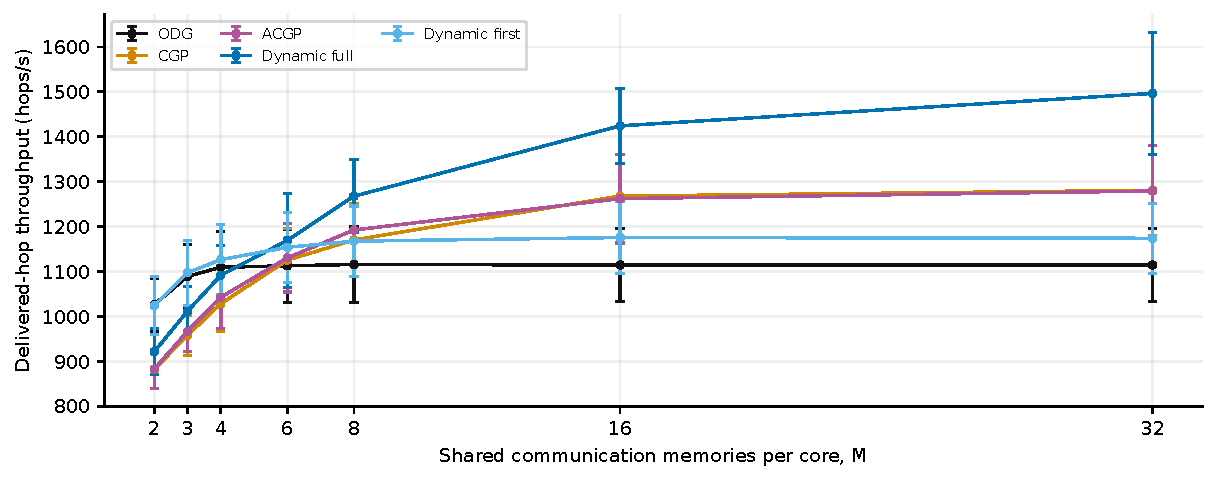
\includegraphics[width=.94\linewidth,height=.255\textheight,keepaspectratio]{figures/memory/mesh_max_reliability_hop_throughput_s.pdf}\captionof{figure}{Run-level mean and sample SD. Shared trace aliases are counted once.}\end{center}
\begin{center}{\scriptsize\setlength{\tabcolsep}{3pt}
\begin{tabular}{lrrrrr}
\toprule
M & ODG & CGP & ACGP & Dynamic full & Dynamic first \\
\midrule
2 & $1026.40\pm59.04$ & $882.23\pm42.95$ & $882.87\pm43.75$ & $921.62\pm51.21$ & $1024.08\pm64.18$ \\
3 & $1089.23\pm71.23$ & $958.29\pm44.43$ & $966.97\pm45.54$ & $1011.72\pm54.42$ & $1097.52\pm72.30$ \\
4 & $1109.46\pm79.89$ & $1028.55\pm62.26$ & $1042.77\pm69.56$ & $1091.69\pm65.83$ & $1126.37\pm77.93$ \\
6 & $1112.74\pm81.07$ & $1125.43\pm69.89$ & $1130.48\pm76.05$ & $1169.36\pm104.01$ & $1154.02\pm77.43$ \\
8 & $1115.70\pm83.77$ & $1170.31\pm81.32$ & $1192.37\pm78.33$ & $1267.63\pm81.19$ & $1167.56\pm78.27$ \\
16 & $1114.48\pm82.08$ & $1267.89\pm91.86$ & $1262.18\pm98.63$ & $1424.19\pm83.30$ & $1175.67\pm79.68$ \\
32 & $1114.48\pm82.08$ & $1280.75\pm100.02$ & $1279.23\pm100.88$ & $1496.50\pm135.82$ & $1174.00\pm77.54$ \\
\bottomrule\end{tabular}}
\captionof{table}{Mean $\pm$ sample SD; n/a denotes a metric outside that policy's instrumentation.}
{\footnotesize\href{https://github.com/sanjeevkrishnaa/Compiler-Driven-ACE/blob/codex/ace-scheduler-correctness/docs/latex/qft96_final/data/memory_mesh_max_reliability_hop_throughput_s.csv}{Exact CSV values and sample counts}}
\end{center}
\subsection*{Completion fraction}
\begin{center}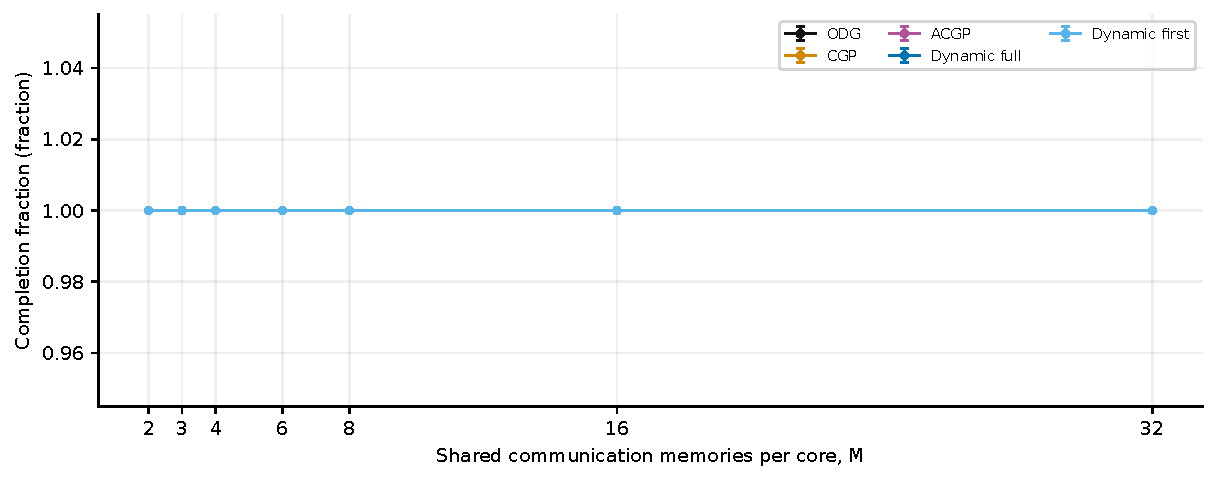
\includegraphics[width=.94\linewidth,height=.255\textheight,keepaspectratio]{figures/memory/mesh_max_reliability_completion_rate.pdf}\captionof{figure}{Run-level mean and sample SD. Shared trace aliases are counted once.}\end{center}
\begin{center}{\scriptsize\setlength{\tabcolsep}{3pt}
\begin{tabular}{lrrrrr}
\toprule
M & ODG & CGP & ACGP & Dynamic full & Dynamic first \\
\midrule
2 & $1.000\pm0.000$ & $1.000\pm0.000$ & $1.000\pm0.000$ & $1.000\pm0.000$ & $1.000\pm0.000$ \\
3 & $1.000\pm0.000$ & $1.000\pm0.000$ & $1.000\pm0.000$ & $1.000\pm0.000$ & $1.000\pm0.000$ \\
4 & $1.000\pm0.000$ & $1.000\pm0.000$ & $1.000\pm0.000$ & $1.000\pm0.000$ & $1.000\pm0.000$ \\
6 & $1.000\pm0.000$ & $1.000\pm0.000$ & $1.000\pm0.000$ & $1.000\pm0.000$ & $1.000\pm0.000$ \\
8 & $1.000\pm0.000$ & $1.000\pm0.000$ & $1.000\pm0.000$ & $1.000\pm0.000$ & $1.000\pm0.000$ \\
16 & $1.000\pm0.000$ & $1.000\pm0.000$ & $1.000\pm0.000$ & $1.000\pm0.000$ & $1.000\pm0.000$ \\
32 & $1.000\pm0.000$ & $1.000\pm0.000$ & $1.000\pm0.000$ & $1.000\pm0.000$ & $1.000\pm0.000$ \\
\bottomrule\end{tabular}}
\captionof{table}{Mean $\pm$ sample SD; n/a denotes a metric outside that policy's instrumentation.}
{\footnotesize\href{https://github.com/sanjeevkrishnaa/Compiler-Driven-ACE/blob/codex/ace-scheduler-correctness/docs/latex/qft96_final/data/memory_mesh_max_reliability_completion_rate.csv}{Exact CSV values and sample counts}}
\end{center}
\clearpage
\subsection*{Maximum admission wait}
\begin{center}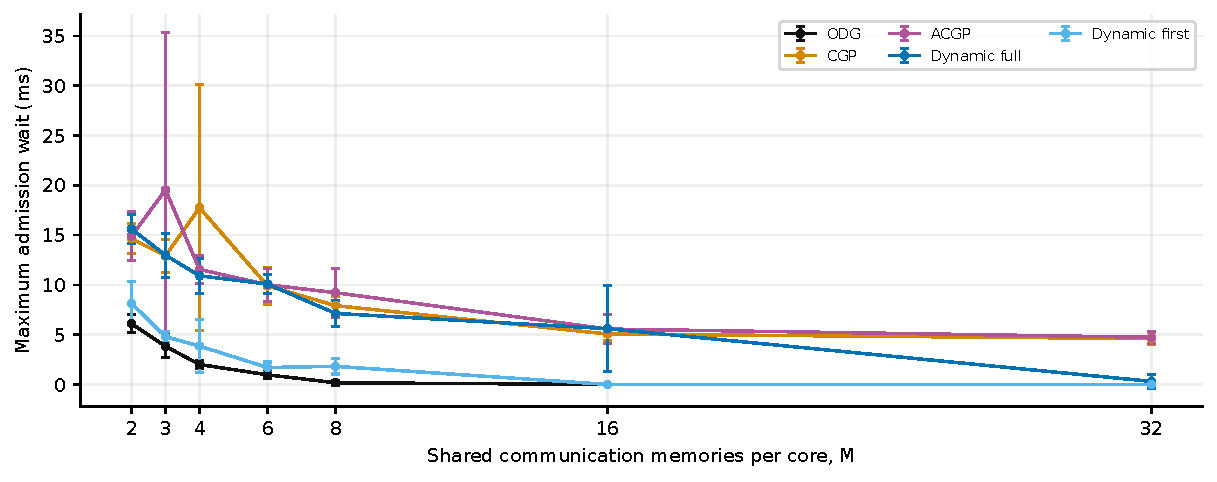
\includegraphics[width=.94\linewidth,height=.255\textheight,keepaspectratio]{figures/memory/mesh_max_reliability_max_admission_wait_ms.pdf}\captionof{figure}{Run-level mean and sample SD. Shared trace aliases are counted once.}\end{center}
\begin{center}{\scriptsize\setlength{\tabcolsep}{3pt}
\begin{tabular}{lrrrrr}
\toprule
M & ODG & CGP & ACGP & Dynamic full & Dynamic first \\
\midrule
2 & $6.117\pm0.926$ & $14.649\pm1.527$ & $14.904\pm2.499$ & $15.617\pm1.419$ & $8.134\pm2.239$ \\
3 & $3.833\pm1.171$ & $12.917\pm1.671$ & $19.542\pm15.834$ & $12.984\pm2.205$ & $4.800\pm0.544$ \\
4 & $2.000\pm0.363$ & $17.760\pm12.335$ & $11.550\pm1.432$ & $10.917\pm1.775$ & $3.850\pm2.657$ \\
6 & $0.9667\pm0.4033$ & $9.900\pm1.891$ & $10.017\pm1.657$ & $10.084\pm0.937$ & $1.700\pm0.551$ \\
8 & $0.1667\pm0.2582$ & $7.917\pm0.941$ & $9.217\pm2.448$ & $7.134\pm1.320$ & $1.817\pm0.771$ \\
16 & $0.0000\pm0.0000$ & $5.067\pm0.656$ & $5.567\pm1.439$ & $5.600\pm4.337$ & $0.0000\pm0.0000$ \\
32 & $0.0000\pm0.0000$ & $4.600\pm0.590$ & $4.733\pm0.589$ & $0.3000\pm0.7349$ & $0.0000\pm0.0000$ \\
\bottomrule\end{tabular}}
\captionof{table}{Mean $\pm$ sample SD; n/a denotes a metric outside that policy's instrumentation.}
{\footnotesize\href{https://github.com/sanjeevkrishnaa/Compiler-Driven-ACE/blob/codex/ace-scheduler-correctness/docs/latex/qft96_final/data/memory_mesh_max_reliability_max_admission_wait_ms.csv}{Exact CSV values and sample counts}}
\end{center}
\subsection*{Requests with admission wait}
\begin{center}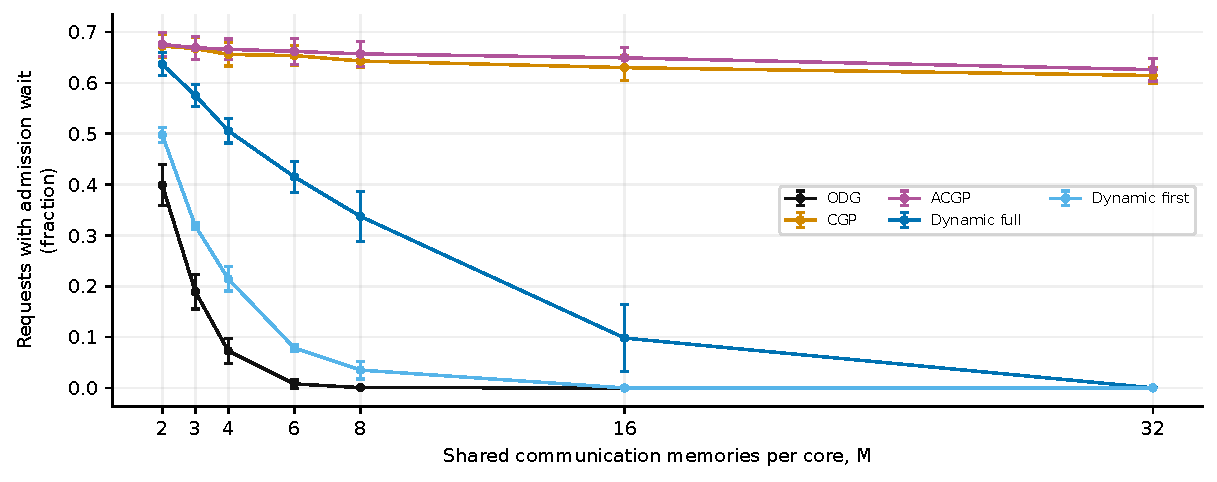
\includegraphics[width=.94\linewidth,height=.255\textheight,keepaspectratio]{figures/memory/mesh_max_reliability_requests_that_waited_fraction.pdf}\captionof{figure}{Run-level mean and sample SD. Shared trace aliases are counted once.}\end{center}
\begin{center}{\scriptsize\setlength{\tabcolsep}{3pt}
\begin{tabular}{lrrrrr}
\toprule
M & ODG & CGP & ACGP & Dynamic full & Dynamic first \\
\midrule
2 & $0.3990\pm0.0399$ & $0.6725\pm0.0233$ & $0.6757\pm0.0238$ & $0.6367\pm0.0229$ & $0.4977\pm0.0147$ \\
3 & $0.1895\pm0.0342$ & $0.6676\pm0.0218$ & $0.6692\pm0.0225$ & $0.5755\pm0.0220$ & $0.3189\pm0.0063$ \\
4 & $0.0726\pm0.0253$ & $0.6560\pm0.0227$ & $0.6661\pm0.0202$ & $0.5057\pm0.0239$ & $0.2143\pm0.0237$ \\
6 & $0.0079\pm0.0095$ & $0.6537\pm0.0191$ & $0.6620\pm0.0253$ & $0.4152\pm0.0299$ & $0.0786\pm0.0065$ \\
8 & $0.0006\pm0.0010$ & $0.6431\pm0.0126$ & $0.6571\pm0.0248$ & $0.3375\pm0.0493$ & $0.0351\pm0.0176$ \\
16 & $0.0000\pm0.0000$ & $0.6300\pm0.0247$ & $0.6493\pm0.0210$ & $0.0981\pm0.0664$ & $0.0000\pm0.0000$ \\
32 & $0.0000\pm0.0000$ & $0.6146\pm0.0158$ & $0.6261\pm0.0224$ & $0.0001\pm0.0002$ & $0.0000\pm0.0000$ \\
\bottomrule\end{tabular}}
\captionof{table}{Mean $\pm$ sample SD; n/a denotes a metric outside that policy's instrumentation.}
{\footnotesize\href{https://github.com/sanjeevkrishnaa/Compiler-Driven-ACE/blob/codex/ace-scheduler-correctness/docs/latex/qft96_final/data/memory_mesh_max_reliability_requests_that_waited_fraction.csv}{Exact CSV values and sample counts}}
\end{center}
\clearpage
\subsection*{Recorded reservation-setup counter}
\begin{center}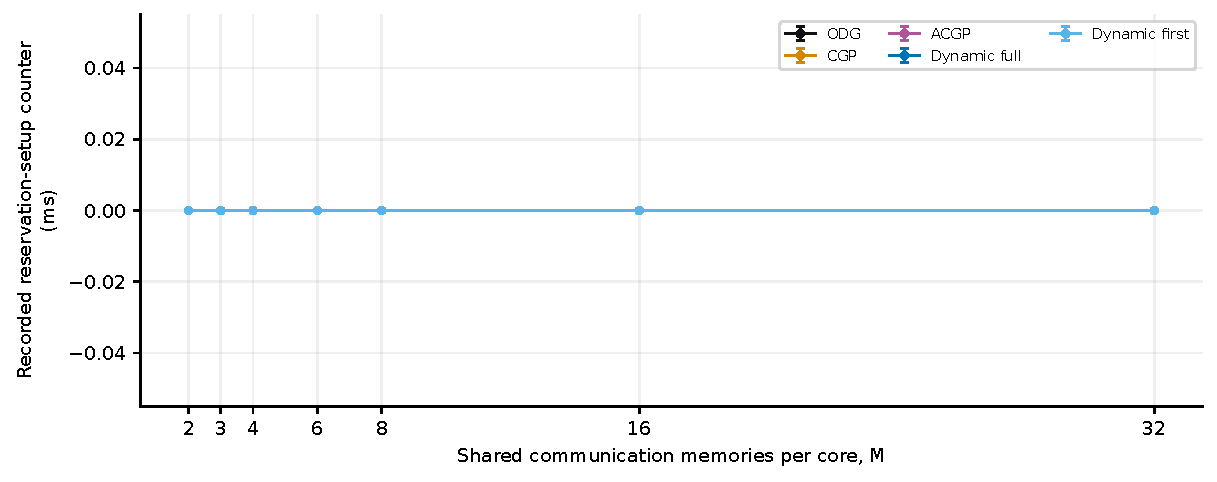
\includegraphics[width=.94\linewidth,height=.255\textheight,keepaspectratio]{figures/memory/mesh_max_reliability_avg_reservation_setup_time_ms.pdf}\captionof{figure}{Run-level mean and sample SD. Shared trace aliases are counted once.}\end{center}
\begin{center}{\scriptsize\setlength{\tabcolsep}{3pt}
\begin{tabular}{lrrrrr}
\toprule
M & ODG & CGP & ACGP & Dynamic full & Dynamic first \\
\midrule
2 & $0.0000\pm0.0000$ & $0.0000\pm0.0000$ & $0.0000\pm0.0000$ & $0.0000\pm0.0000$ & $0.0000\pm0.0000$ \\
3 & $0.0000\pm0.0000$ & $0.0000\pm0.0000$ & $0.0000\pm0.0000$ & $0.0000\pm0.0000$ & $0.0000\pm0.0000$ \\
4 & $0.0000\pm0.0000$ & $0.0000\pm0.0000$ & $0.0000\pm0.0000$ & $0.0000\pm0.0000$ & $0.0000\pm0.0000$ \\
6 & $0.0000\pm0.0000$ & $0.0000\pm0.0000$ & $0.0000\pm0.0000$ & $0.0000\pm0.0000$ & $0.0000\pm0.0000$ \\
8 & $0.0000\pm0.0000$ & $0.0000\pm0.0000$ & $0.0000\pm0.0000$ & $0.0000\pm0.0000$ & $0.0000\pm0.0000$ \\
16 & $0.0000\pm0.0000$ & $0.0000\pm0.0000$ & $0.0000\pm0.0000$ & $0.0000\pm0.0000$ & $0.0000\pm0.0000$ \\
32 & $0.0000\pm0.0000$ & $0.0000\pm0.0000$ & $0.0000\pm0.0000$ & $0.0000\pm0.0000$ & $0.0000\pm0.0000$ \\
\bottomrule\end{tabular}}
\captionof{table}{Mean $\pm$ sample SD; n/a denotes a metric outside that policy's instrumentation.}
{\footnotesize\href{https://github.com/sanjeevkrishnaa/Compiler-Driven-ACE/blob/codex/ace-scheduler-correctness/docs/latex/qft96_final/data/memory_mesh_max_reliability_avg_reservation_setup_time_ms.csv}{Exact CSV values and sample counts}}
\end{center}
\subsection*{Mean generation/service time}
\begin{center}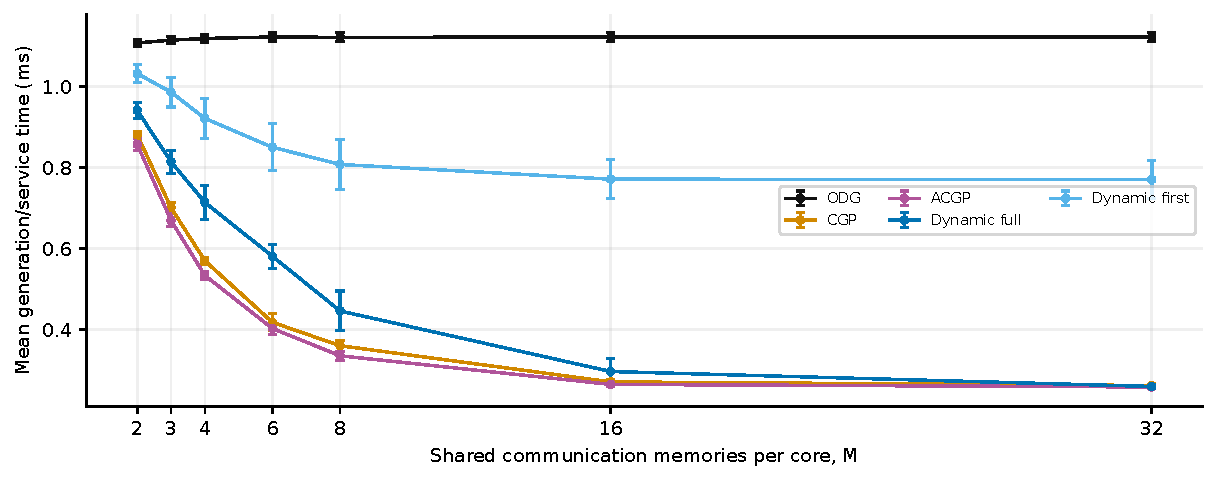
\includegraphics[width=.94\linewidth,height=.255\textheight,keepaspectratio]{figures/memory/mesh_max_reliability_avg_entanglement_generation_time_ms.pdf}\captionof{figure}{Run-level mean and sample SD. Shared trace aliases are counted once.}\end{center}
\begin{center}{\scriptsize\setlength{\tabcolsep}{3pt}
\begin{tabular}{lrrrrr}
\toprule
M & ODG & CGP & ACGP & Dynamic full & Dynamic first \\
\midrule
2 & $1.108\pm0.009$ & $0.8811\pm0.0091$ & $0.8574\pm0.0149$ & $0.9414\pm0.0199$ & $1.032\pm0.022$ \\
3 & $1.115\pm0.008$ & $0.7011\pm0.0124$ & $0.6697\pm0.0160$ & $0.8145\pm0.0287$ & $0.9864\pm0.0367$ \\
4 & $1.119\pm0.011$ & $0.5702\pm0.0081$ & $0.5339\pm0.0101$ & $0.7144\pm0.0423$ & $0.9214\pm0.0489$ \\
6 & $1.122\pm0.011$ & $0.4182\pm0.0210$ & $0.4029\pm0.0156$ & $0.5810\pm0.0301$ & $0.8502\pm0.0579$ \\
8 & $1.121\pm0.011$ & $0.3604\pm0.0137$ & $0.3355\pm0.0116$ & $0.4462\pm0.0493$ & $0.8078\pm0.0626$ \\
16 & $1.122\pm0.012$ & $0.2711\pm0.0070$ & $0.2649\pm0.0050$ & $0.2968\pm0.0322$ & $0.7715\pm0.0476$ \\
32 & $1.122\pm0.012$ & $0.2622\pm0.0035$ & $0.2586\pm0.0044$ & $0.2598\pm0.0009$ & $0.7706\pm0.0465$ \\
\bottomrule\end{tabular}}
\captionof{table}{Mean $\pm$ sample SD; n/a denotes a metric outside that policy's instrumentation.}
{\footnotesize\href{https://github.com/sanjeevkrishnaa/Compiler-Driven-ACE/blob/codex/ace-scheduler-correctness/docs/latex/qft96_final/data/memory_mesh_max_reliability_avg_entanglement_generation_time_ms.csv}{Exact CSV values and sample counts}}
\end{center}
\clearpage
\subsection*{Recorded retry-wait time}
\begin{center}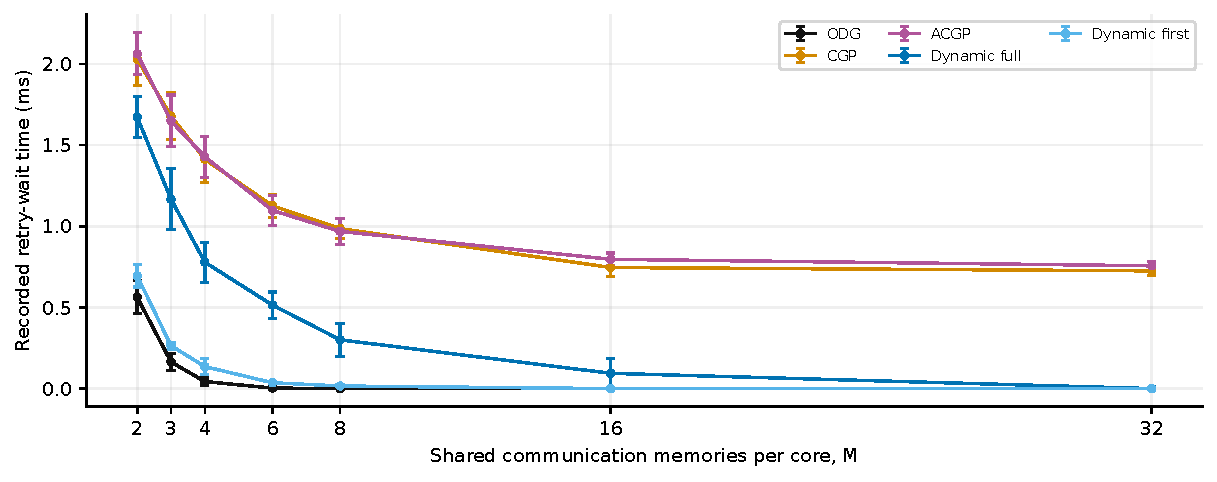
\includegraphics[width=.94\linewidth,height=.255\textheight,keepaspectratio]{figures/memory/mesh_max_reliability_avg_retry_wait_time_ms.pdf}\captionof{figure}{Run-level mean and sample SD. Shared trace aliases are counted once.}\end{center}
\begin{center}{\scriptsize\setlength{\tabcolsep}{3pt}
\begin{tabular}{lrrrrr}
\toprule
M & ODG & CGP & ACGP & Dynamic full & Dynamic first \\
\midrule
2 & $0.5628\pm0.1018$ & $2.030\pm0.165$ & $2.063\pm0.128$ & $1.671\pm0.127$ & $0.6942\pm0.0683$ \\
3 & $0.1644\pm0.0510$ & $1.679\pm0.145$ & $1.649\pm0.159$ & $1.167\pm0.189$ & $0.2641\pm0.0227$ \\
4 & $0.0435\pm0.0225$ & $1.413\pm0.142$ & $1.428\pm0.128$ & $0.7787\pm0.1226$ & $0.1358\pm0.0479$ \\
6 & $0.0033\pm0.0041$ & $1.126\pm0.070$ & $1.098\pm0.091$ & $0.5148\pm0.0806$ & $0.0362\pm0.0031$ \\
8 & $0.0001\pm0.0002$ & $0.9859\pm0.0611$ & $0.9685\pm0.0814$ & $0.3007\pm0.1004$ & $0.0162\pm0.0110$ \\
16 & $0.0000\pm0.0000$ & $0.7461\pm0.0552$ & $0.7966\pm0.0388$ & $0.0944\pm0.0934$ & $0.0000\pm0.0000$ \\
32 & $0.0000\pm0.0000$ & $0.7254\pm0.0289$ & $0.7565\pm0.0270$ & $0.0001\pm0.0002$ & $0.0000\pm0.0000$ \\
\bottomrule\end{tabular}}
\captionof{table}{Mean $\pm$ sample SD; n/a denotes a metric outside that policy's instrumentation.}
{\footnotesize\href{https://github.com/sanjeevkrishnaa/Compiler-Driven-ACE/blob/codex/ace-scheduler-correctness/docs/latex/qft96_final/data/memory_mesh_max_reliability_avg_retry_wait_time_ms.csv}{Exact CSV values and sample counts}}
\end{center}
\subsection*{Request retries}
\begin{center}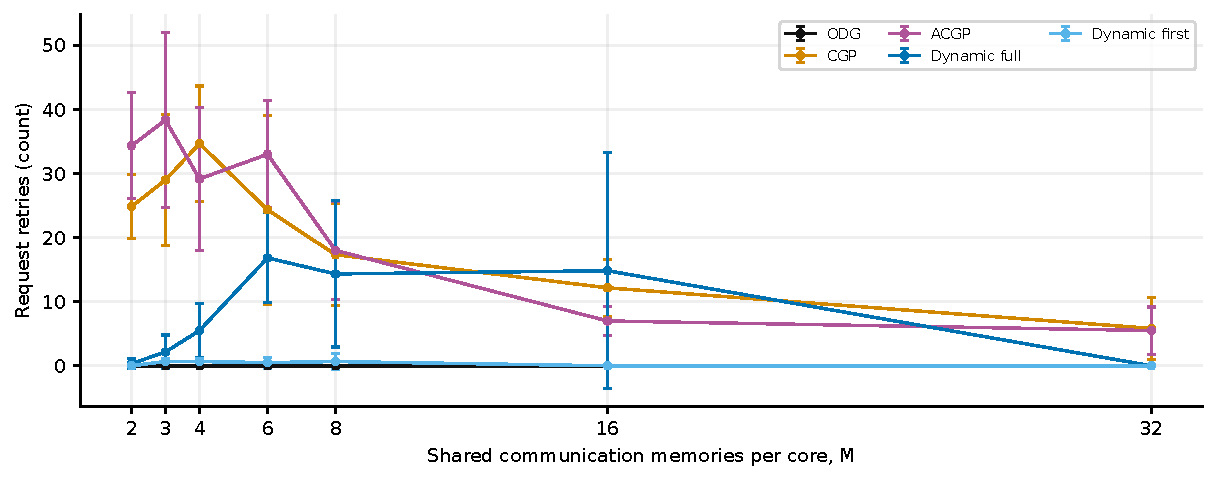
\includegraphics[width=.94\linewidth,height=.255\textheight,keepaspectratio]{figures/memory/mesh_max_reliability_total_retries.pdf}\captionof{figure}{Run-level mean and sample SD. Shared trace aliases are counted once.}\end{center}
\begin{center}{\scriptsize\setlength{\tabcolsep}{3pt}
\begin{tabular}{lrrrrr}
\toprule
M & ODG & CGP & ACGP & Dynamic full & Dynamic first \\
\midrule
2 & $0.0000\pm0.0000$ & $24.833\pm5.037$ & $34.333\pm8.238$ & $0.3333\pm0.8165$ & $0.0000\pm0.0000$ \\
3 & $0.0000\pm0.0000$ & $29.000\pm10.276$ & $38.333\pm13.692$ & $2.167\pm2.639$ & $0.6667\pm0.5164$ \\
4 & $0.0000\pm0.0000$ & $34.667\pm8.981$ & $29.167\pm11.197$ & $5.500\pm4.231$ & $0.6667\pm0.5164$ \\
6 & $0.0000\pm0.0000$ & $24.333\pm14.747$ & $33.000\pm8.343$ & $16.833\pm7.026$ & $0.5000\pm0.8367$ \\
8 & $0.0000\pm0.0000$ & $17.333\pm7.941$ & $18.000\pm7.616$ & $14.333\pm11.396$ & $0.6667\pm1.2111$ \\
16 & $0.0000\pm0.0000$ & $12.167\pm4.446$ & $7.000\pm2.280$ & $14.833\pm18.411$ & $0.0000\pm0.0000$ \\
32 & $0.0000\pm0.0000$ & $5.833\pm4.792$ & $5.500\pm3.674$ & $0.0000\pm0.0000$ & $0.0000\pm0.0000$ \\
\bottomrule\end{tabular}}
\captionof{table}{Mean $\pm$ sample SD; n/a denotes a metric outside that policy's instrumentation.}
{\footnotesize\href{https://github.com/sanjeevkrishnaa/Compiler-Driven-ACE/blob/codex/ace-scheduler-correctness/docs/latex/qft96_final/data/memory_mesh_max_reliability_total_retries.csv}{Exact CSV values and sample counts}}
\end{center}
\clearpage
\subsection*{Requests with retries}
\begin{center}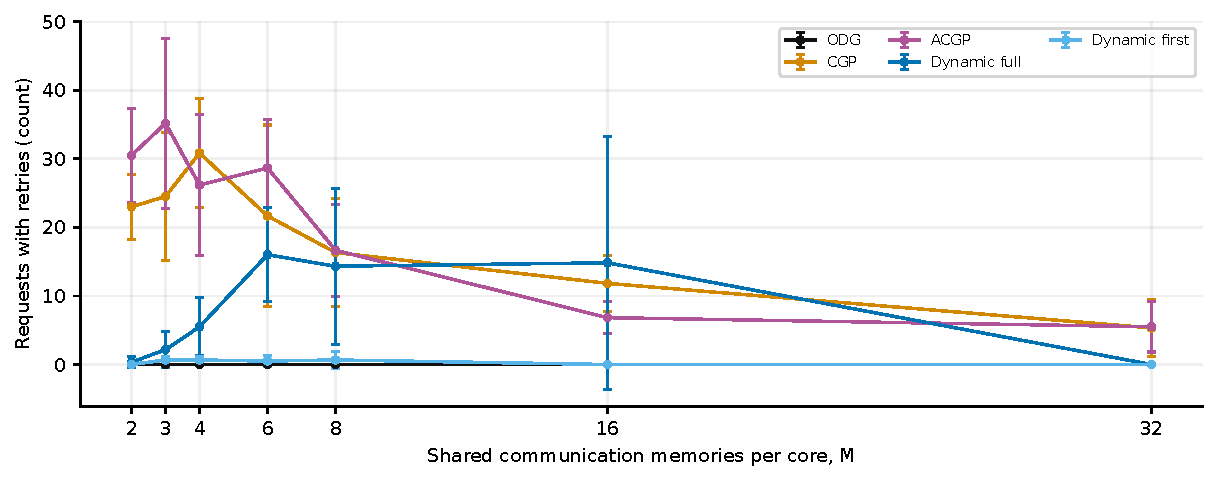
\includegraphics[width=.94\linewidth,height=.255\textheight,keepaspectratio]{figures/memory/mesh_max_reliability_requests_with_retries.pdf}\captionof{figure}{Run-level mean and sample SD. Shared trace aliases are counted once.}\end{center}
\begin{center}{\scriptsize\setlength{\tabcolsep}{3pt}
\begin{tabular}{lrrrrr}
\toprule
M & ODG & CGP & ACGP & Dynamic full & Dynamic first \\
\midrule
2 & $0.0000\pm0.0000$ & $23.000\pm4.733$ & $30.500\pm6.834$ & $0.3333\pm0.8165$ & $0.0000\pm0.0000$ \\
3 & $0.0000\pm0.0000$ & $24.500\pm9.311$ & $35.167\pm12.368$ & $2.167\pm2.639$ & $0.6667\pm0.5164$ \\
4 & $0.0000\pm0.0000$ & $30.833\pm7.935$ & $26.167\pm10.304$ & $5.500\pm4.231$ & $0.6667\pm0.5164$ \\
6 & $0.0000\pm0.0000$ & $21.667\pm13.261$ & $28.667\pm7.033$ & $16.000\pm6.841$ & $0.5000\pm0.8367$ \\
8 & $0.0000\pm0.0000$ & $16.333\pm7.815$ & $16.667\pm6.713$ & $14.333\pm11.396$ & $0.6667\pm1.2111$ \\
16 & $0.0000\pm0.0000$ & $11.833\pm4.070$ & $6.833\pm2.317$ & $14.833\pm18.411$ & $0.0000\pm0.0000$ \\
32 & $0.0000\pm0.0000$ & $5.333\pm4.179$ & $5.500\pm3.674$ & $0.0000\pm0.0000$ & $0.0000\pm0.0000$ \\
\bottomrule\end{tabular}}
\captionof{table}{Mean $\pm$ sample SD; n/a denotes a metric outside that policy's instrumentation.}
{\footnotesize\href{https://github.com/sanjeevkrishnaa/Compiler-Driven-ACE/blob/codex/ace-scheduler-correctness/docs/latex/qft96_final/data/memory_mesh_max_reliability_requests_with_retries.csv}{Exact CSV values and sample counts}}
\end{center}
\subsection*{Native-protocol generated-pair counter}
\begin{center}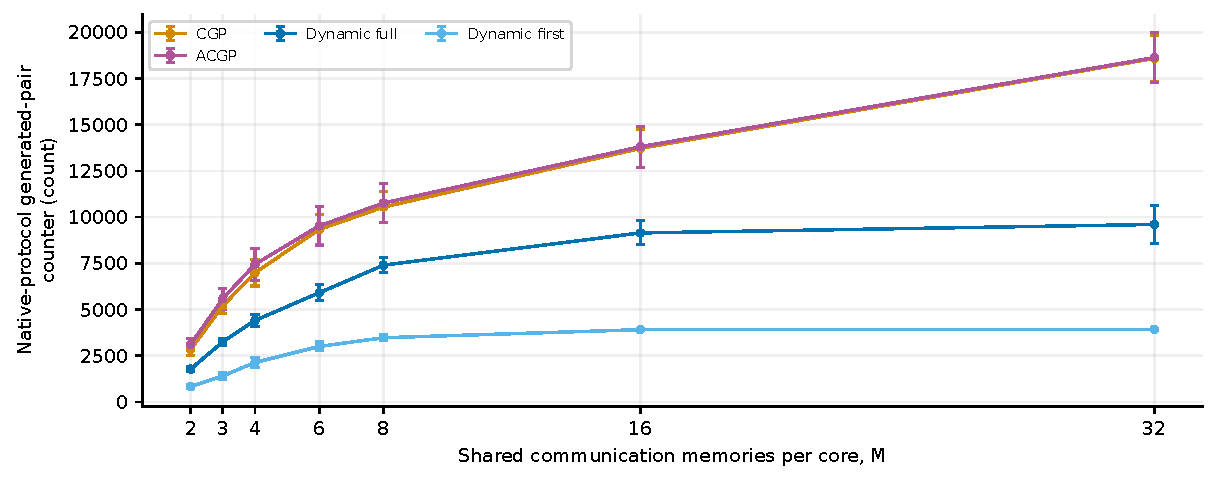
\includegraphics[width=.94\linewidth,height=.255\textheight,keepaspectratio]{figures/memory/mesh_max_reliability_protocol_generated_pairs.pdf}\captionof{figure}{Run-level mean and sample SD. Shared trace aliases are counted once.}\end{center}
\begin{center}{\scriptsize\setlength{\tabcolsep}{3pt}
\begin{tabular}{lrrrrr}
\toprule
M & ODG & CGP & ACGP & Dynamic full & Dynamic first \\
\midrule
2 & n/a & $2842.00\pm307.94$ & $3124.67\pm322.02$ & $1781.00\pm139.31$ & $824.00\pm107.34$ \\
3 & n/a & $5211.67\pm407.39$ & $5587.00\pm574.65$ & $3259.00\pm197.48$ & $1415.00\pm198.65$ \\
4 & n/a & $6991.67\pm714.96$ & $7446.00\pm856.72$ & $4407.33\pm320.29$ & $2137.00\pm262.01$ \\
6 & n/a & $9335.00\pm814.32$ & $9526.33\pm1058.00$ & $5911.00\pm434.10$ & $3003.67\pm240.88$ \\
8 & n/a & $10544.67\pm836.13$ & $10759.33\pm1040.82$ & $7400.33\pm412.53$ & $3476.33\pm174.27$ \\
16 & n/a & $13720.00\pm1047.76$ & $13807.33\pm1103.02$ & $9145.33\pm648.48$ & $3912.67\pm26.85$ \\
32 & n/a & $18591.67\pm1242.86$ & $18631.33\pm1365.72$ & $9604.33\pm1028.20$ & $3930.00\pm0.00$ \\
\bottomrule\end{tabular}}
\captionof{table}{Mean $\pm$ sample SD; n/a denotes a metric outside that policy's instrumentation.}
{\footnotesize\href{https://github.com/sanjeevkrishnaa/Compiler-Driven-ACE/blob/codex/ace-scheduler-correctness/docs/latex/qft96_final/data/memory_mesh_max_reliability_protocol_generated_pairs.csv}{Exact CSV values and sample counts}}
\end{center}
\clearpage
\subsection*{Native-protocol used-pair counter}
\begin{center}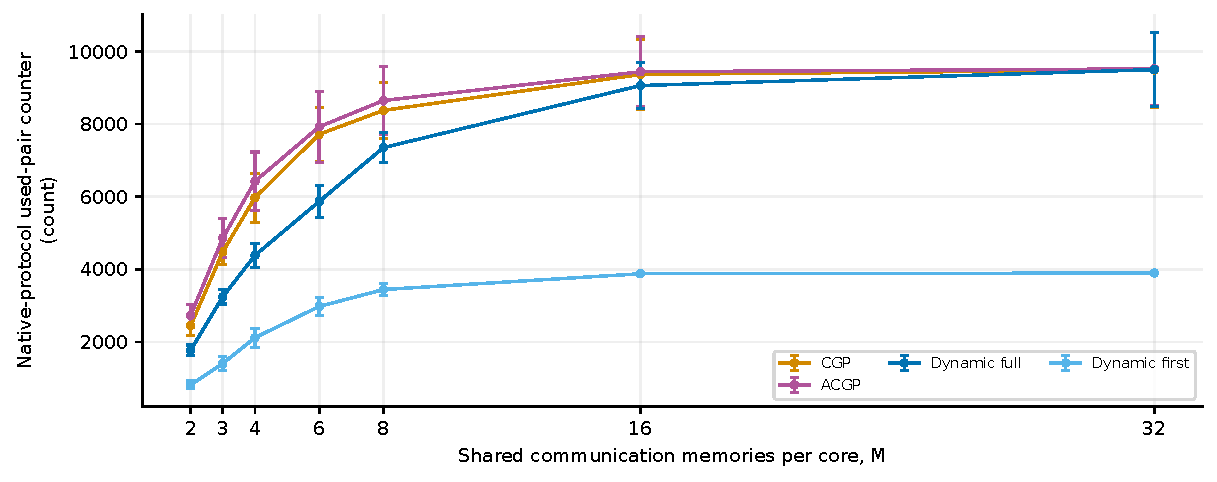
\includegraphics[width=.94\linewidth,height=.255\textheight,keepaspectratio]{figures/memory/mesh_max_reliability_protocol_used_pairs.pdf}\captionof{figure}{Run-level mean and sample SD. Shared trace aliases are counted once.}\end{center}
\begin{center}{\scriptsize\setlength{\tabcolsep}{3pt}
\begin{tabular}{lrrrrr}
\toprule
M & ODG & CGP & ACGP & Dynamic full & Dynamic first \\
\midrule
2 & n/a & $2452.67\pm277.59$ & $2736.67\pm304.14$ & $1776.00\pm141.64$ & $820.00\pm107.06$ \\
3 & n/a & $4487.00\pm356.85$ & $4864.00\pm531.77$ & $3246.00\pm199.74$ & $1406.67\pm198.69$ \\
4 & n/a & $5971.67\pm671.66$ & $6422.00\pm808.09$ & $4383.67\pm322.68$ & $2117.67\pm264.39$ \\
6 & n/a & $7718.00\pm736.63$ & $7923.33\pm977.25$ & $5869.00\pm439.91$ & $2978.00\pm240.03$ \\
8 & n/a & $8375.33\pm765.19$ & $8647.67\pm928.99$ & $7350.00\pm413.76$ & $3443.33\pm173.60$ \\
16 & n/a & $9365.00\pm954.88$ & $9439.00\pm959.38$ & $9059.67\pm642.97$ & $3878.67\pm31.66$ \\
32 & n/a & $9492.00\pm1021.95$ & $9519.00\pm1006.04$ & $9499.00\pm1014.96$ & $3898.00\pm7.48$ \\
\bottomrule\end{tabular}}
\captionof{table}{Mean $\pm$ sample SD; n/a denotes a metric outside that policy's instrumentation.}
{\footnotesize\href{https://github.com/sanjeevkrishnaa/Compiler-Driven-ACE/blob/codex/ace-scheduler-correctness/docs/latex/qft96_final/data/memory_mesh_max_reliability_protocol_used_pairs.csv}{Exact CSV values and sample counts}}
\end{center}
\subsection*{Native-protocol unused-pair counter}
\begin{center}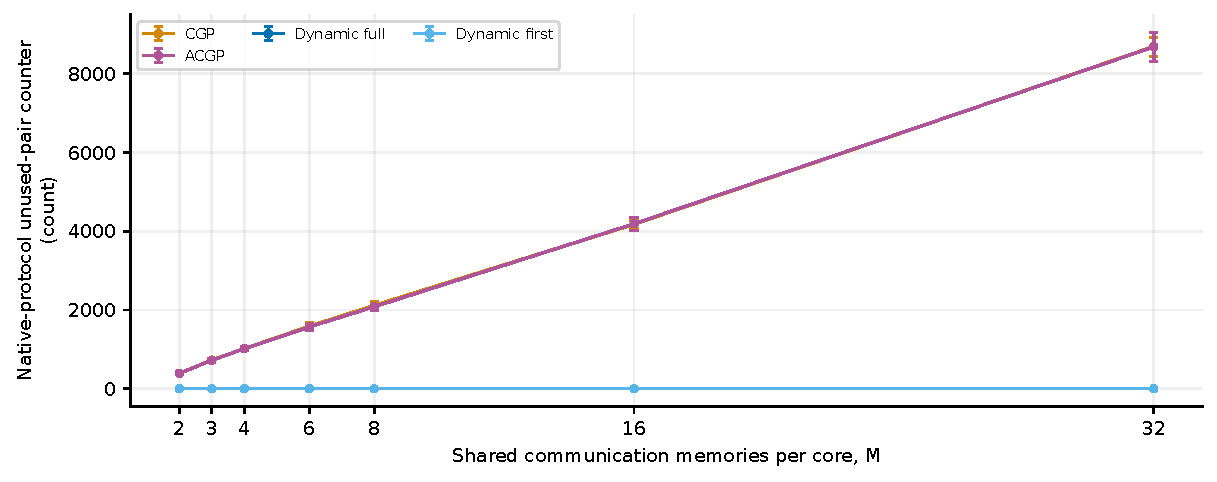
\includegraphics[width=.94\linewidth,height=.255\textheight,keepaspectratio]{figures/memory/mesh_max_reliability_protocol_unused_pairs.pdf}\captionof{figure}{Run-level mean and sample SD. Shared trace aliases are counted once.}\end{center}
\begin{center}{\scriptsize\setlength{\tabcolsep}{3pt}
\begin{tabular}{lrrrrr}
\toprule
M & ODG & CGP & ACGP & Dynamic full & Dynamic first \\
\midrule
2 & n/a & $388.33\pm33.19$ & $391.00\pm26.80$ & $0.0000\pm0.0000$ & $0.0000\pm0.0000$ \\
3 & n/a & $727.33\pm50.42$ & $722.00\pm42.82$ & $0.0000\pm0.0000$ & $0.0000\pm0.0000$ \\
4 & n/a & $1016.00\pm47.85$ & $1020.00\pm55.37$ & $0.0000\pm0.0000$ & $0.0000\pm0.0000$ \\
6 & n/a & $1585.00\pm88.75$ & $1569.33\pm83.17$ & $0.0000\pm0.0000$ & $0.0000\pm0.0000$ \\
8 & n/a & $2115.67\pm89.80$ & $2082.33\pm100.87$ & $0.0000\pm0.0000$ & $0.0000\pm0.0000$ \\
16 & n/a & $4178.00\pm107.12$ & $4188.67\pm162.00$ & $0.0000\pm0.0000$ & $0.0000\pm0.0000$ \\
32 & n/a & $8690.00\pm241.49$ & $8684.00\pm368.55$ & $0.0000\pm0.0000$ & $0.0000\pm0.0000$ \\
\bottomrule\end{tabular}}
\captionof{table}{Mean $\pm$ sample SD; n/a denotes a metric outside that policy's instrumentation.}
{\footnotesize\href{https://github.com/sanjeevkrishnaa/Compiler-Driven-ACE/blob/codex/ace-scheduler-correctness/docs/latex/qft96_final/data/memory_mesh_max_reliability_protocol_unused_pairs.csv}{Exact CSV values and sample counts}}
\end{center}
\clearpage
\subsection*{Scheduled compiler preparations}
\begin{center}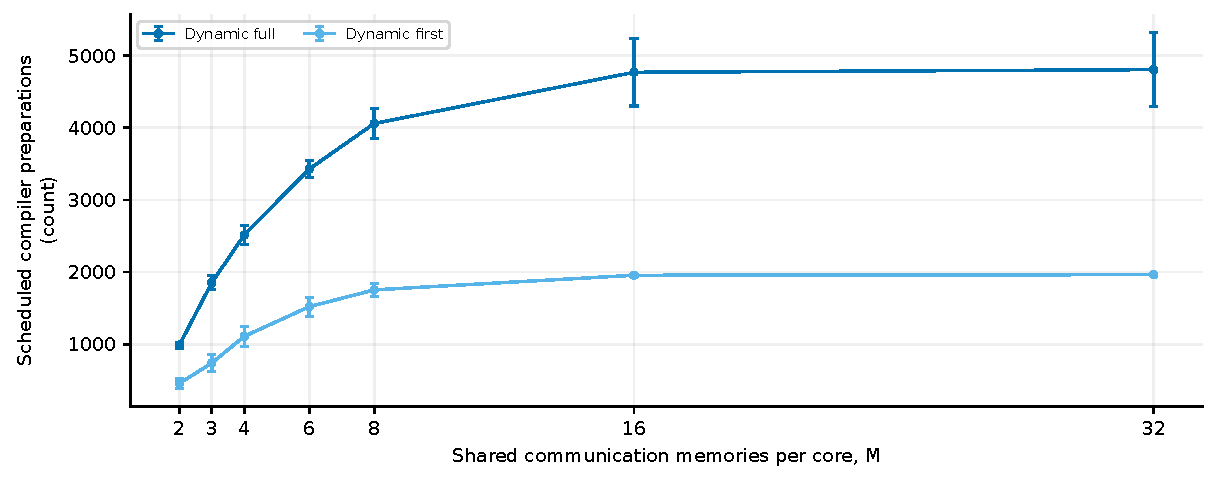
\includegraphics[width=.94\linewidth,height=.255\textheight,keepaspectratio]{figures/memory/mesh_max_reliability_scheduled_preparations.pdf}\captionof{figure}{Run-level mean and sample SD. Shared trace aliases are counted once.}\end{center}
\begin{center}{\scriptsize\setlength{\tabcolsep}{3pt}
\begin{tabular}{lrrrrr}
\toprule
M & ODG & CGP & ACGP & Dynamic full & Dynamic first \\
\midrule
2 & n/a & n/a & n/a & $989.33\pm40.32$ & $459.00\pm73.91$ \\
3 & n/a & n/a & n/a & $1853.67\pm93.98$ & $740.67\pm114.71$ \\
4 & n/a & n/a & n/a & $2514.67\pm128.78$ & $1111.67\pm136.75$ \\
6 & n/a & n/a & n/a & $3427.67\pm121.31$ & $1521.33\pm133.30$ \\
8 & n/a & n/a & n/a & $4058.00\pm204.64$ & $1754.33\pm90.12$ \\
16 & n/a & n/a & n/a & $4767.00\pm466.48$ & $1956.33\pm13.43$ \\
32 & n/a & n/a & n/a & $4804.00\pm516.61$ & $1965.00\pm0.00$ \\
\bottomrule\end{tabular}}
\captionof{table}{Mean $\pm$ sample SD; n/a denotes a metric outside that policy's instrumentation.}
{\footnotesize\href{https://github.com/sanjeevkrishnaa/Compiler-Driven-ACE/blob/codex/ace-scheduler-correctness/docs/latex/qft96_final/data/memory_mesh_max_reliability_scheduled_preparations.csv}{Exact CSV values and sample counts}}
\end{center}
\subsection*{Planner-blocked preparations}
\begin{center}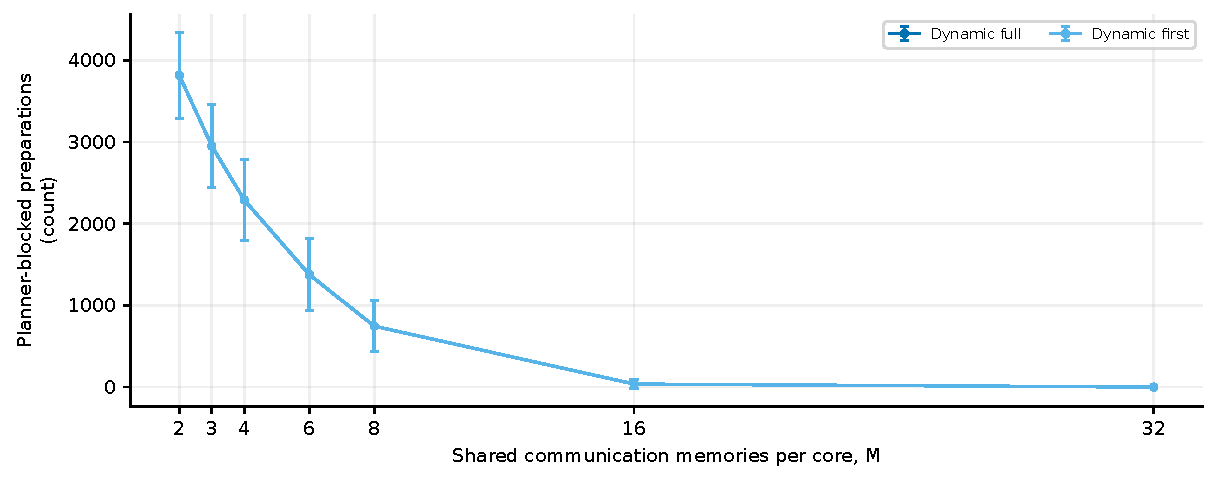
\includegraphics[width=.94\linewidth,height=.255\textheight,keepaspectratio]{figures/memory/mesh_max_reliability_planner_blocked_preparations.pdf}\captionof{figure}{Run-level mean and sample SD. Shared trace aliases are counted once.}\end{center}
\begin{center}{\scriptsize\setlength{\tabcolsep}{3pt}
\begin{tabular}{lrrrrr}
\toprule
M & ODG & CGP & ACGP & Dynamic full & Dynamic first \\
\midrule
2 & n/a & n/a & n/a & $3814.67\pm526.61$ & $3814.67\pm526.61$ \\
3 & n/a & n/a & n/a & $2950.33\pm511.09$ & $2950.33\pm511.09$ \\
4 & n/a & n/a & n/a & $2289.33\pm493.48$ & $2289.33\pm493.48$ \\
6 & n/a & n/a & n/a & $1376.33\pm441.29$ & $1376.33\pm441.29$ \\
8 & n/a & n/a & n/a & $746.00\pm312.22$ & $746.00\pm312.22$ \\
16 & n/a & n/a & n/a & $37.000\pm57.320$ & $37.000\pm57.320$ \\
32 & n/a & n/a & n/a & $0.0000\pm0.0000$ & $0.0000\pm0.0000$ \\
\bottomrule\end{tabular}}
\captionof{table}{Mean $\pm$ sample SD; n/a denotes a metric outside that policy's instrumentation.}
{\footnotesize\href{https://github.com/sanjeevkrishnaa/Compiler-Driven-ACE/blob/codex/ace-scheduler-correctness/docs/latex/qft96_final/data/memory_mesh_max_reliability_planner_blocked_preparations.csv}{Exact CSV values and sample counts}}
\end{center}
\clearpage
\subsection*{Planner peak compiler memory}
\begin{center}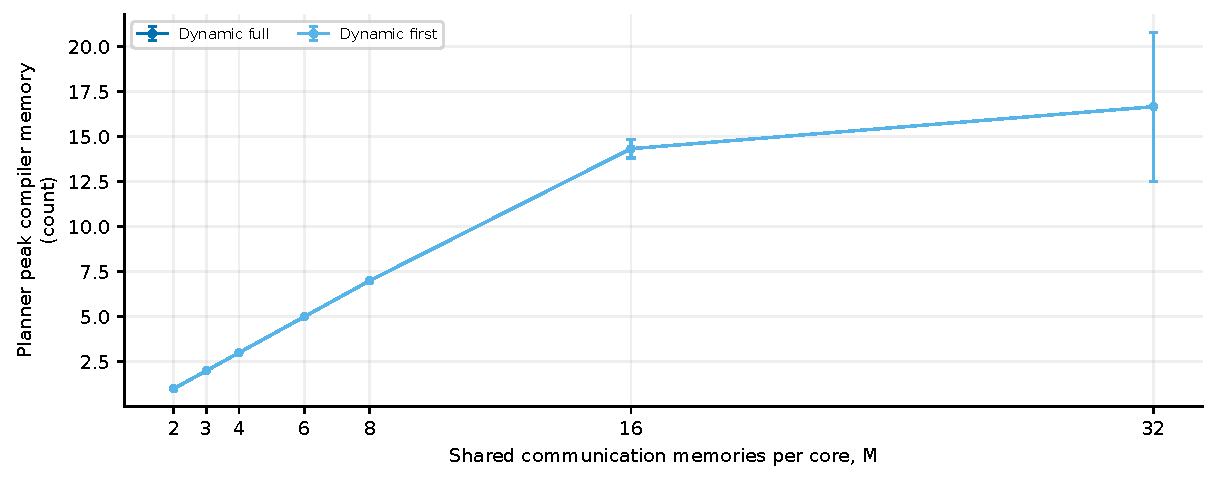
\includegraphics[width=.94\linewidth,height=.255\textheight,keepaspectratio]{figures/memory/mesh_max_reliability_planner_peak_compiler_memory_per_core.pdf}\captionof{figure}{Run-level mean and sample SD. Shared trace aliases are counted once.}\end{center}
\begin{center}{\scriptsize\setlength{\tabcolsep}{3pt}
\begin{tabular}{lrrrrr}
\toprule
M & ODG & CGP & ACGP & Dynamic full & Dynamic first \\
\midrule
2 & n/a & n/a & n/a & $1.000\pm0.000$ & $1.000\pm0.000$ \\
3 & n/a & n/a & n/a & $2.000\pm0.000$ & $2.000\pm0.000$ \\
4 & n/a & n/a & n/a & $3.000\pm0.000$ & $3.000\pm0.000$ \\
6 & n/a & n/a & n/a & $5.000\pm0.000$ & $5.000\pm0.000$ \\
8 & n/a & n/a & n/a & $7.000\pm0.000$ & $7.000\pm0.000$ \\
16 & n/a & n/a & n/a & $14.333\pm0.516$ & $14.333\pm0.516$ \\
32 & n/a & n/a & n/a & $16.667\pm4.131$ & $16.667\pm4.131$ \\
\bottomrule\end{tabular}}
\captionof{table}{Mean $\pm$ sample SD; n/a denotes a metric outside that policy's instrumentation.}
{\footnotesize\href{https://github.com/sanjeevkrishnaa/Compiler-Driven-ACE/blob/codex/ace-scheduler-correctness/docs/latex/qft96_final/data/memory_mesh_max_reliability_planner_peak_compiler_memory_per_core.csv}{Exact CSV values and sample counts}}
\end{center}
\subsection*{Compiler preparation admission attempts}
\begin{center}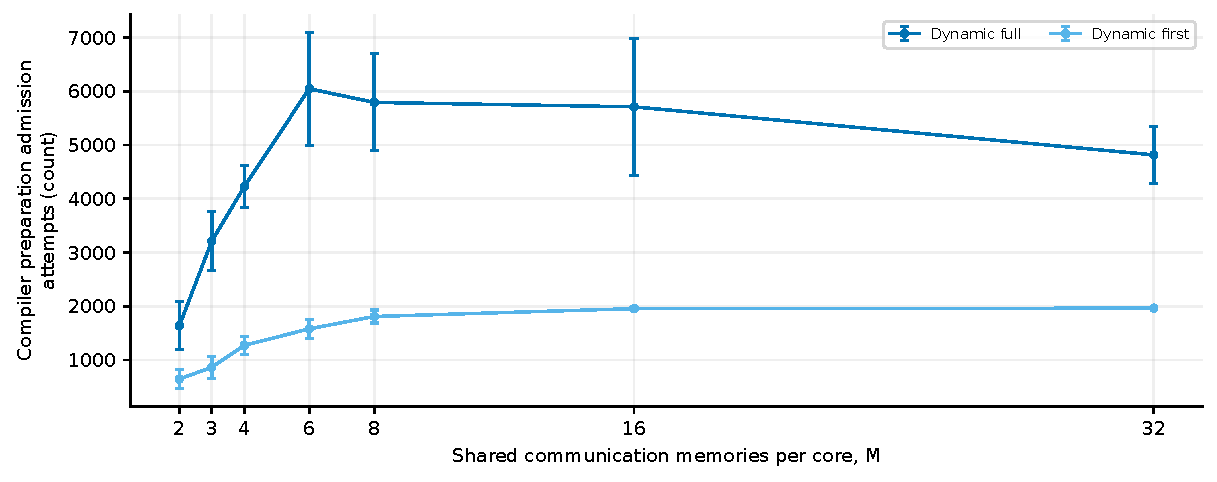
\includegraphics[width=.94\linewidth,height=.255\textheight,keepaspectratio]{figures/memory/mesh_max_reliability_runtime_admission_attempts.pdf}\captionof{figure}{Run-level mean and sample SD. Shared trace aliases are counted once.}\end{center}
\begin{center}{\scriptsize\setlength{\tabcolsep}{3pt}
\begin{tabular}{lrrrrr}
\toprule
M & ODG & CGP & ACGP & Dynamic full & Dynamic first \\
\midrule
2 & n/a & n/a & n/a & $1637.17\pm444.13$ & $645.33\pm179.47$ \\
3 & n/a & n/a & n/a & $3211.83\pm545.75$ & $865.33\pm208.75$ \\
4 & n/a & n/a & n/a & $4224.67\pm394.72$ & $1272.67\pm162.88$ \\
6 & n/a & n/a & n/a & $6046.33\pm1049.48$ & $1580.17\pm175.32$ \\
8 & n/a & n/a & n/a & $5792.00\pm902.29$ & $1809.67\pm121.38$ \\
16 & n/a & n/a & n/a & $5709.83\pm1271.16$ & $1956.33\pm13.43$ \\
32 & n/a & n/a & n/a & $4816.00\pm533.66$ & $1965.00\pm0.00$ \\
\bottomrule\end{tabular}}
\captionof{table}{Mean $\pm$ sample SD; n/a denotes a metric outside that policy's instrumentation.}
{\footnotesize\href{https://github.com/sanjeevkrishnaa/Compiler-Driven-ACE/blob/codex/ace-scheduler-correctness/docs/latex/qft96_final/data/memory_mesh_max_reliability_runtime_admission_attempts.csv}{Exact CSV values and sample counts}}
\end{center}
\clearpage
\subsection*{Launched compiler preparations}
\begin{center}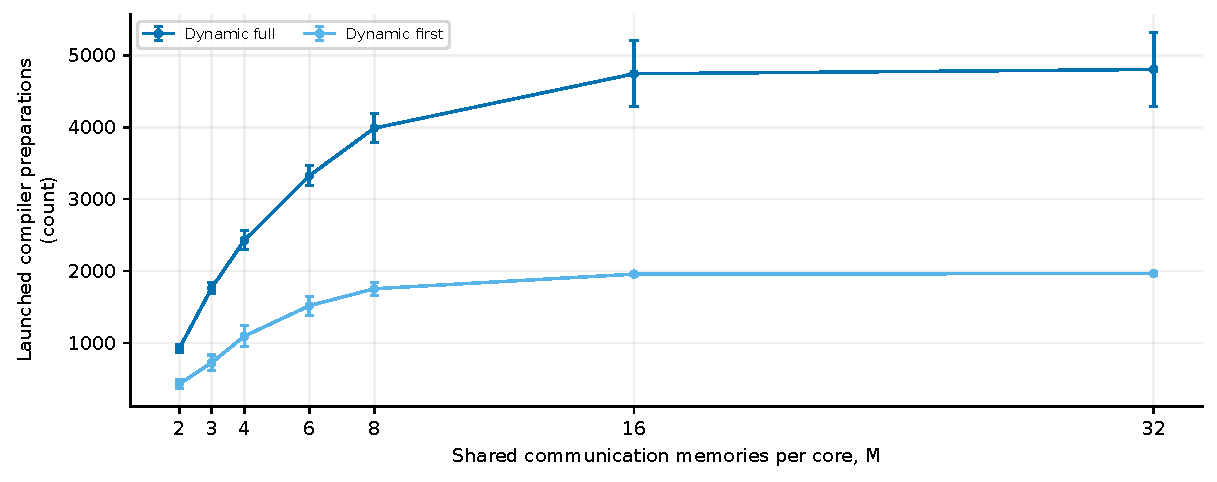
\includegraphics[width=.94\linewidth,height=.255\textheight,keepaspectratio]{figures/memory/mesh_max_reliability_runtime_launched_preparations.pdf}\captionof{figure}{Run-level mean and sample SD. Shared trace aliases are counted once.}\end{center}
\begin{center}{\scriptsize\setlength{\tabcolsep}{3pt}
\begin{tabular}{lrrrrr}
\toprule
M & ODG & CGP & ACGP & Dynamic full & Dynamic first \\
\midrule
2 & n/a & n/a & n/a & $921.67\pm58.13$ & $427.67\pm66.07$ \\
3 & n/a & n/a & n/a & $1765.83\pm72.51$ & $724.83\pm106.59$ \\
4 & n/a & n/a & n/a & $2425.00\pm132.21$ & $1092.33\pm144.19$ \\
6 & n/a & n/a & n/a & $3324.17\pm138.93$ & $1516.17\pm130.90$ \\
8 & n/a & n/a & n/a & $3987.17\pm202.64$ & $1753.00\pm88.67$ \\
16 & n/a & n/a & n/a & $4743.67\pm459.23$ & $1956.33\pm13.43$ \\
32 & n/a & n/a & n/a & $4804.00\pm516.61$ & $1965.00\pm0.00$ \\
\bottomrule\end{tabular}}
\captionof{table}{Mean $\pm$ sample SD; n/a denotes a metric outside that policy's instrumentation.}
{\footnotesize\href{https://github.com/sanjeevkrishnaa/Compiler-Driven-ACE/blob/codex/ace-scheduler-correctness/docs/latex/qft96_final/data/memory_mesh_max_reliability_runtime_launched_preparations.csv}{Exact CSV values and sample counts}}
\end{center}
\subsection*{Accepted compiler preparations}
\begin{center}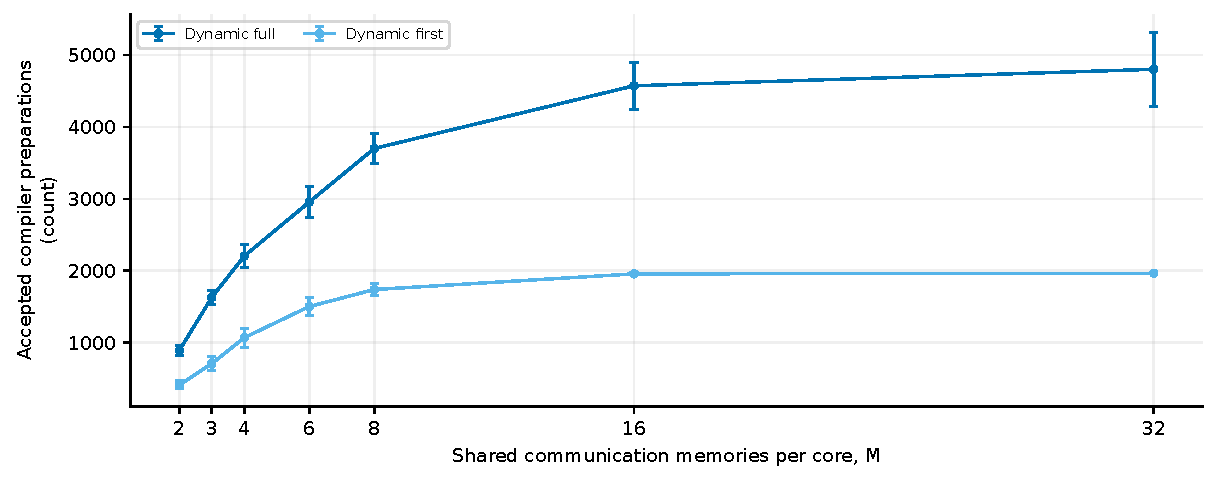
\includegraphics[width=.94\linewidth,height=.255\textheight,keepaspectratio]{figures/memory/mesh_max_reliability_runtime_accepted_preparations.pdf}\captionof{figure}{Run-level mean and sample SD. Shared trace aliases are counted once.}\end{center}
\begin{center}{\scriptsize\setlength{\tabcolsep}{3pt}
\begin{tabular}{lrrrrr}
\toprule
M & ODG & CGP & ACGP & Dynamic full & Dynamic first \\
\midrule
2 & n/a & n/a & n/a & $890.50\pm69.65$ & $412.00\pm53.67$ \\
3 & n/a & n/a & n/a & $1629.50\pm98.74$ & $707.50\pm99.32$ \\
4 & n/a & n/a & n/a & $2203.67\pm160.15$ & $1068.50\pm131.00$ \\
6 & n/a & n/a & n/a & $2955.50\pm217.05$ & $1501.83\pm120.44$ \\
8 & n/a & n/a & n/a & $3700.17\pm206.27$ & $1738.17\pm87.14$ \\
16 & n/a & n/a & n/a & $4572.67\pm324.24$ & $1956.33\pm13.43$ \\
32 & n/a & n/a & n/a & $4802.17\pm514.10$ & $1965.00\pm0.00$ \\
\bottomrule\end{tabular}}
\captionof{table}{Mean $\pm$ sample SD; n/a denotes a metric outside that policy's instrumentation.}
{\footnotesize\href{https://github.com/sanjeevkrishnaa/Compiler-Driven-ACE/blob/codex/ace-scheduler-correctness/docs/latex/qft96_final/data/memory_mesh_max_reliability_runtime_accepted_preparations.csv}{Exact CSV values and sample counts}}
\end{center}
\clearpage
\subsection*{Rejected compiler preparations}
\begin{center}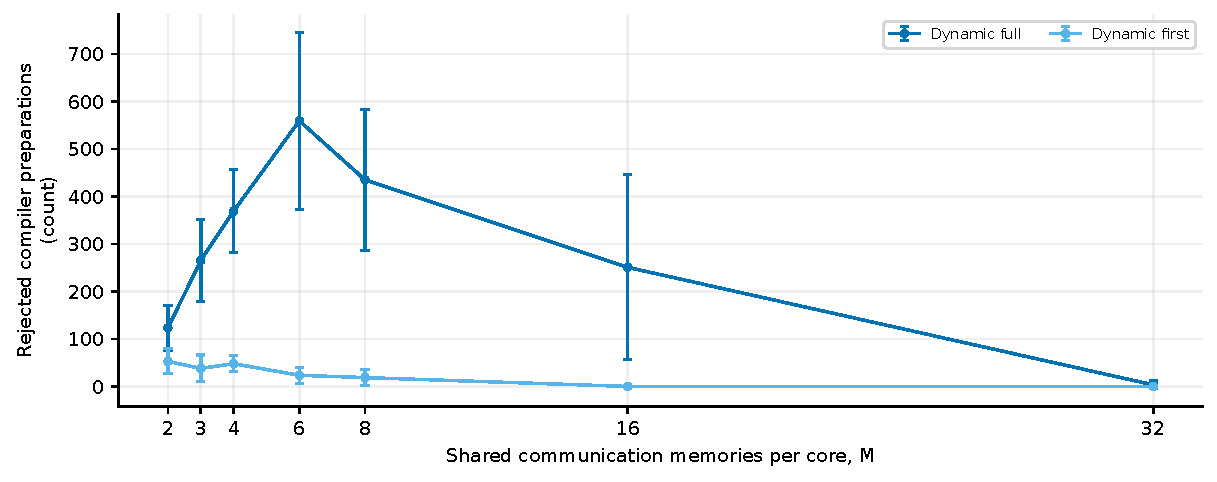
\includegraphics[width=.94\linewidth,height=.255\textheight,keepaspectratio]{figures/memory/mesh_max_reliability_runtime_rejected_preparations.pdf}\captionof{figure}{Run-level mean and sample SD. Shared trace aliases are counted once.}\end{center}
\begin{center}{\scriptsize\setlength{\tabcolsep}{3pt}
\begin{tabular}{lrrrrr}
\toprule
M & ODG & CGP & ACGP & Dynamic full & Dynamic first \\
\midrule
2 & n/a & n/a & n/a & $123.33\pm47.77$ & $52.833\pm26.279$ \\
3 & n/a & n/a & n/a & $265.17\pm86.44$ & $38.000\pm28.270$ \\
4 & n/a & n/a & n/a & $369.17\pm87.73$ & $47.833\pm16.928$ \\
6 & n/a & n/a & n/a & $559.33\pm186.30$ & $23.500\pm16.670$ \\
8 & n/a & n/a & n/a & $435.00\pm148.47$ & $18.667\pm16.269$ \\
16 & n/a & n/a & n/a & $250.83\pm194.71$ & $0.0000\pm0.0000$ \\
32 & n/a & n/a & n/a & $3.333\pm8.165$ & $0.0000\pm0.0000$ \\
\bottomrule\end{tabular}}
\captionof{table}{Mean $\pm$ sample SD; n/a denotes a metric outside that policy's instrumentation.}
{\footnotesize\href{https://github.com/sanjeevkrishnaa/Compiler-Driven-ACE/blob/codex/ace-scheduler-correctness/docs/latex/qft96_final/data/memory_mesh_max_reliability_runtime_rejected_preparations.csv}{Exact CSV values and sample counts}}
\end{center}
\subsection*{Compiler-ready request count}
\begin{center}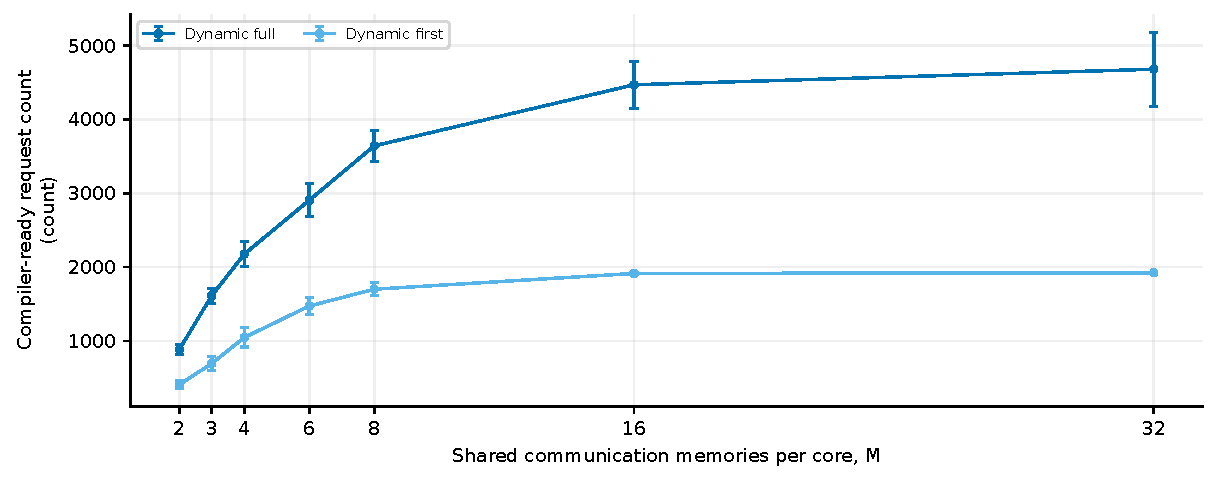
\includegraphics[width=.94\linewidth,height=.255\textheight,keepaspectratio]{figures/memory/mesh_max_reliability_pregenerated_hits.pdf}\captionof{figure}{Run-level mean and sample SD. Shared trace aliases are counted once.}\end{center}
\begin{center}{\scriptsize\setlength{\tabcolsep}{3pt}
\begin{tabular}{lrrrrr}
\toprule
M & ODG & CGP & ACGP & Dynamic full & Dynamic first \\
\midrule
2 & n/a & n/a & n/a & $883.83\pm71.90$ & $406.33\pm53.81$ \\
3 & n/a & n/a & n/a & $1612.83\pm102.72$ & $695.67\pm99.26$ \\
4 & n/a & n/a & n/a & $2174.83\pm165.06$ & $1046.50\pm129.10$ \\
6 & n/a & n/a & n/a & $2904.17\pm222.73$ & $1472.17\pm120.51$ \\
8 & n/a & n/a & n/a & $3640.50\pm210.55$ & $1700.00\pm84.87$ \\
16 & n/a & n/a & n/a & $4467.67\pm317.29$ & $1913.50\pm11.74$ \\
32 & n/a & n/a & n/a & $4678.33\pm499.33$ & $1922.83\pm4.88$ \\
\bottomrule\end{tabular}}
\captionof{table}{Mean $\pm$ sample SD; n/a denotes a metric outside that policy's instrumentation.}
{\footnotesize\href{https://github.com/sanjeevkrishnaa/Compiler-Driven-ACE/blob/codex/ace-scheduler-correctness/docs/latex/qft96_final/data/memory_mesh_max_reliability_pregenerated_hits.csv}{Exact CSV values and sample counts}}
\end{center}
\clearpage
\subsection*{Intended compiler-hit count}
\begin{center}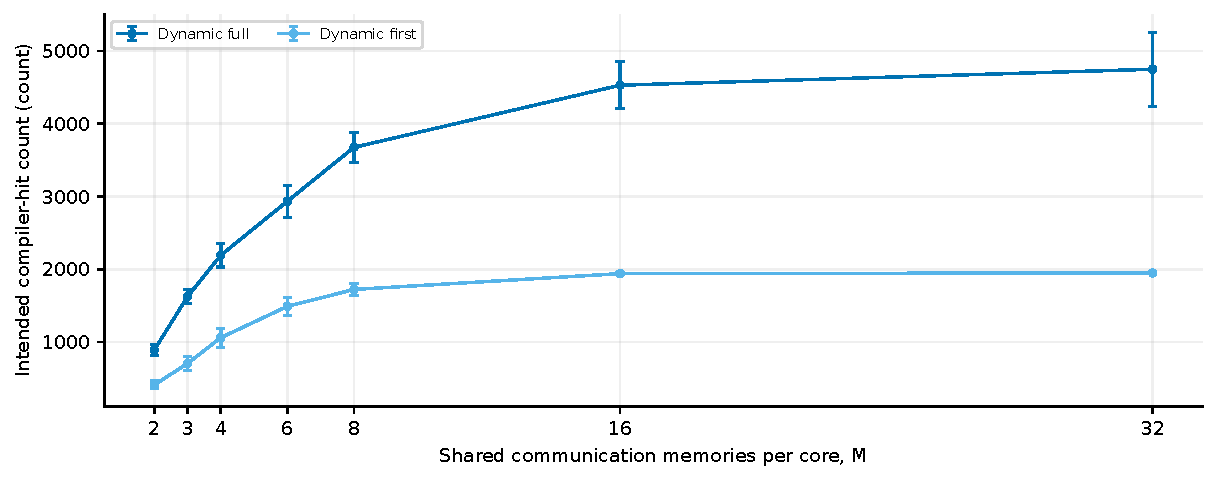
\includegraphics[width=.94\linewidth,height=.255\textheight,keepaspectratio]{figures/memory/mesh_max_reliability_intended_request_hits.pdf}\captionof{figure}{Run-level mean and sample SD. Shared trace aliases are counted once.}\end{center}
\begin{center}{\scriptsize\setlength{\tabcolsep}{3pt}
\begin{tabular}{lrrrrr}
\toprule
M & ODG & CGP & ACGP & Dynamic full & Dynamic first \\
\midrule
2 & n/a & n/a & n/a & $888.00\pm70.82$ & $410.00\pm53.53$ \\
3 & n/a & n/a & n/a & $1623.00\pm99.87$ & $703.33\pm99.35$ \\
4 & n/a & n/a & n/a & $2191.83\pm161.34$ & $1058.83\pm132.19$ \\
6 & n/a & n/a & n/a & $2934.50\pm219.96$ & $1489.00\pm120.01$ \\
8 & n/a & n/a & n/a & $3675.00\pm206.88$ & $1721.67\pm86.80$ \\
16 & n/a & n/a & n/a & $4529.83\pm321.49$ & $1939.33\pm15.83$ \\
32 & n/a & n/a & n/a & $4749.50\pm507.48$ & $1949.00\pm3.74$ \\
\bottomrule\end{tabular}}
\captionof{table}{Mean $\pm$ sample SD; n/a denotes a metric outside that policy's instrumentation.}
{\footnotesize\href{https://github.com/sanjeevkrishnaa/Compiler-Driven-ACE/blob/codex/ace-scheduler-correctness/docs/latex/qft96_final/data/memory_mesh_max_reliability_intended_request_hits.csv}{Exact CSV values and sample counts}}
\end{center}
\subsection*{Compiler-not-ready request count}
\begin{center}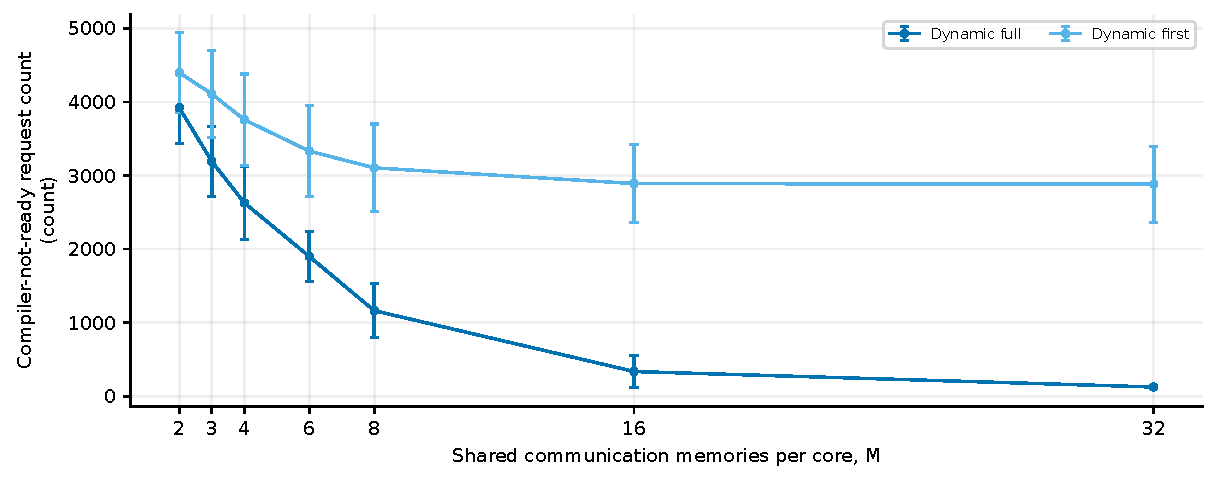
\includegraphics[width=.94\linewidth,height=.255\textheight,keepaspectratio]{figures/memory/mesh_max_reliability_compiler_not_ready_requests.pdf}\captionof{figure}{Run-level mean and sample SD. Shared trace aliases are counted once.}\end{center}
\begin{center}{\scriptsize\setlength{\tabcolsep}{3pt}
\begin{tabular}{lrrrrr}
\toprule
M & ODG & CGP & ACGP & Dynamic full & Dynamic first \\
\midrule
2 & n/a & n/a & n/a & $3920.17\pm483.16$ & $4397.67\pm547.88$ \\
3 & n/a & n/a & n/a & $3191.17\pm471.80$ & $4108.33\pm587.20$ \\
4 & n/a & n/a & n/a & $2629.17\pm495.18$ & $3757.50\pm621.78$ \\
6 & n/a & n/a & n/a & $1899.83\pm336.84$ & $3331.83\pm616.83$ \\
8 & n/a & n/a & n/a & $1163.50\pm370.53$ & $3104.00\pm596.23$ \\
16 & n/a & n/a & n/a & $336.33\pm218.81$ & $2890.50\pm526.92$ \\
32 & n/a & n/a & n/a & $125.67\pm23.46$ & $2881.17\pm514.07$ \\
\bottomrule\end{tabular}}
\captionof{table}{Mean $\pm$ sample SD; n/a denotes a metric outside that policy's instrumentation.}
{\footnotesize\href{https://github.com/sanjeevkrishnaa/Compiler-Driven-ACE/blob/codex/ace-scheduler-correctness/docs/latex/qft96_final/data/memory_mesh_max_reliability_compiler_not_ready_requests.csv}{Exact CSV values and sample counts}}
\end{center}
\clearpage
\subsection*{Late compiler-pair uses}
\begin{center}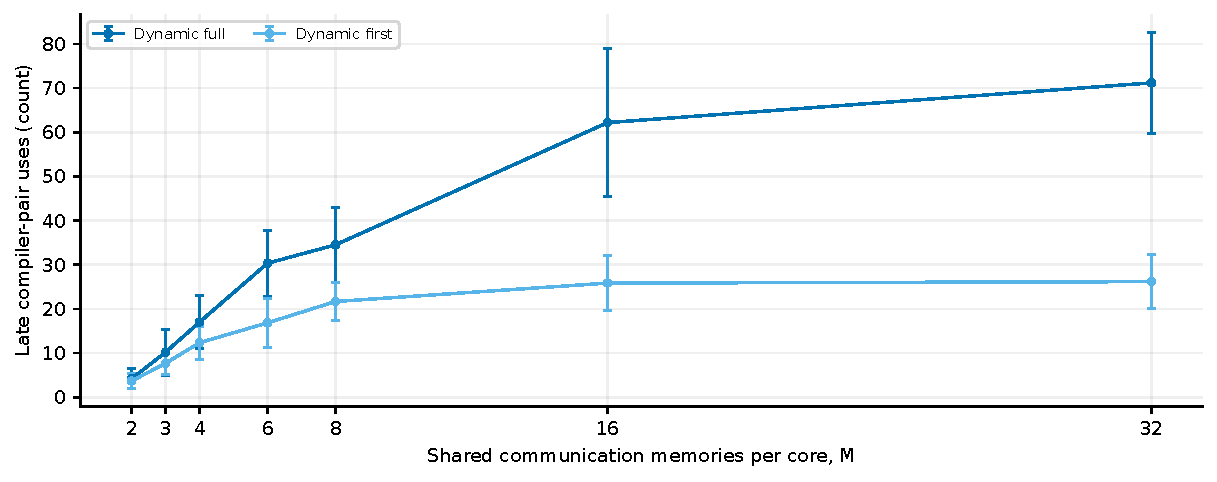
\includegraphics[width=.94\linewidth,height=.255\textheight,keepaspectratio]{figures/memory/mesh_max_reliability_late_compiler_pair_uses.pdf}\captionof{figure}{Run-level mean and sample SD. Shared trace aliases are counted once.}\end{center}
\begin{center}{\scriptsize\setlength{\tabcolsep}{3pt}
\begin{tabular}{lrrrrr}
\toprule
M & ODG & CGP & ACGP & Dynamic full & Dynamic first \\
\midrule
2 & n/a & n/a & n/a & $4.167\pm2.229$ & $3.667\pm1.751$ \\
3 & n/a & n/a & n/a & $10.167\pm5.231$ & $7.667\pm2.422$ \\
4 & n/a & n/a & n/a & $17.000\pm6.033$ & $12.333\pm3.724$ \\
6 & n/a & n/a & n/a & $30.333\pm7.474$ & $16.833\pm5.601$ \\
8 & n/a & n/a & n/a & $34.500\pm8.550$ & $21.667\pm4.274$ \\
16 & n/a & n/a & n/a & $62.167\pm16.774$ & $25.833\pm6.242$ \\
32 & n/a & n/a & n/a & $71.167\pm11.444$ & $26.167\pm6.047$ \\
\bottomrule\end{tabular}}
\captionof{table}{Mean $\pm$ sample SD; n/a denotes a metric outside that policy's instrumentation.}
{\footnotesize\href{https://github.com/sanjeevkrishnaa/Compiler-Driven-ACE/blob/codex/ace-scheduler-correctness/docs/latex/qft96_final/data/memory_mesh_max_reliability_late_compiler_pair_uses.csv}{Exact CSV values and sample counts}}
\end{center}
\subsection*{Compiler fallback count}
\begin{center}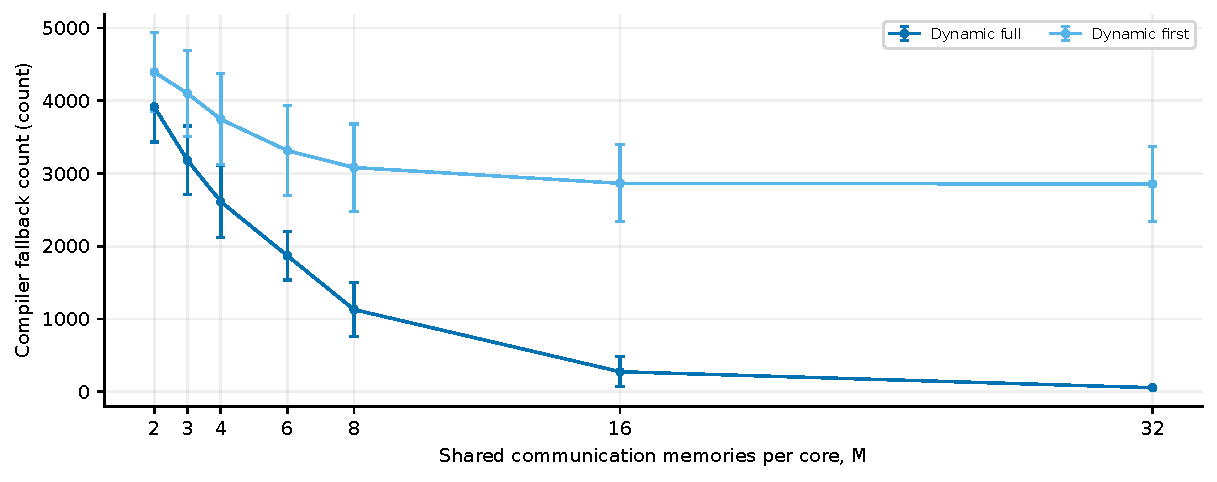
\includegraphics[width=.94\linewidth,height=.255\textheight,keepaspectratio]{figures/memory/mesh_max_reliability_on_demand_fallbacks.pdf}\captionof{figure}{Run-level mean and sample SD. Shared trace aliases are counted once.}\end{center}
\begin{center}{\scriptsize\setlength{\tabcolsep}{3pt}
\begin{tabular}{lrrrrr}
\toprule
M & ODG & CGP & ACGP & Dynamic full & Dynamic first \\
\midrule
2 & n/a & n/a & n/a & $3916.00\pm483.09$ & $4394.00\pm547.21$ \\
3 & n/a & n/a & n/a & $3181.00\pm472.11$ & $4100.67\pm586.59$ \\
4 & n/a & n/a & n/a & $2612.17\pm497.82$ & $3745.17\pm624.79$ \\
6 & n/a & n/a & n/a & $1869.50\pm334.25$ & $3315.00\pm617.38$ \\
8 & n/a & n/a & n/a & $1129.00\pm367.35$ & $3082.33\pm598.72$ \\
16 & n/a & n/a & n/a & $274.17\pm207.89$ & $2864.67\pm529.00$ \\
32 & n/a & n/a & n/a & $54.500\pm14.419$ & $2855.00\pm515.63$ \\
\bottomrule\end{tabular}}
\captionof{table}{Mean $\pm$ sample SD; n/a denotes a metric outside that policy's instrumentation.}
{\footnotesize\href{https://github.com/sanjeevkrishnaa/Compiler-Driven-ACE/blob/codex/ace-scheduler-correctness/docs/latex/qft96_final/data/memory_mesh_max_reliability_on_demand_fallbacks.csv}{Exact CSV values and sample counts}}
\end{center}
\clearpage
\subsection*{Generated compiler pairs}
\begin{center}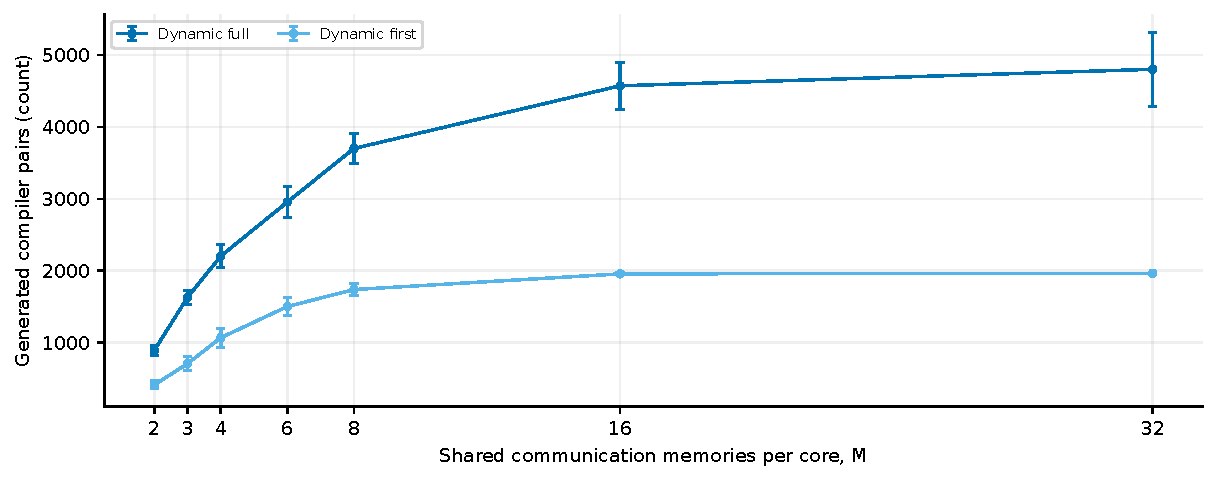
\includegraphics[width=.94\linewidth,height=.255\textheight,keepaspectratio]{figures/memory/mesh_max_reliability_generated_compiler_pairs.pdf}\captionof{figure}{Run-level mean and sample SD. Shared trace aliases are counted once.}\end{center}
\begin{center}{\scriptsize\setlength{\tabcolsep}{3pt}
\begin{tabular}{lrrrrr}
\toprule
M & ODG & CGP & ACGP & Dynamic full & Dynamic first \\
\midrule
2 & n/a & n/a & n/a & $890.50\pm69.65$ & $412.00\pm53.67$ \\
3 & n/a & n/a & n/a & $1629.50\pm98.74$ & $707.50\pm99.32$ \\
4 & n/a & n/a & n/a & $2203.67\pm160.15$ & $1068.50\pm131.00$ \\
6 & n/a & n/a & n/a & $2955.50\pm217.05$ & $1501.83\pm120.44$ \\
8 & n/a & n/a & n/a & $3700.17\pm206.27$ & $1738.17\pm87.14$ \\
16 & n/a & n/a & n/a & $4572.67\pm324.24$ & $1956.33\pm13.43$ \\
32 & n/a & n/a & n/a & $4802.17\pm514.10$ & $1965.00\pm0.00$ \\
\bottomrule\end{tabular}}
\captionof{table}{Mean $\pm$ sample SD; n/a denotes a metric outside that policy's instrumentation.}
{\footnotesize\href{https://github.com/sanjeevkrishnaa/Compiler-Driven-ACE/blob/codex/ace-scheduler-correctness/docs/latex/qft96_final/data/memory_mesh_max_reliability_generated_compiler_pairs.csv}{Exact CSV values and sample counts}}
\end{center}
\subsection*{Used compiler pairs}
\begin{center}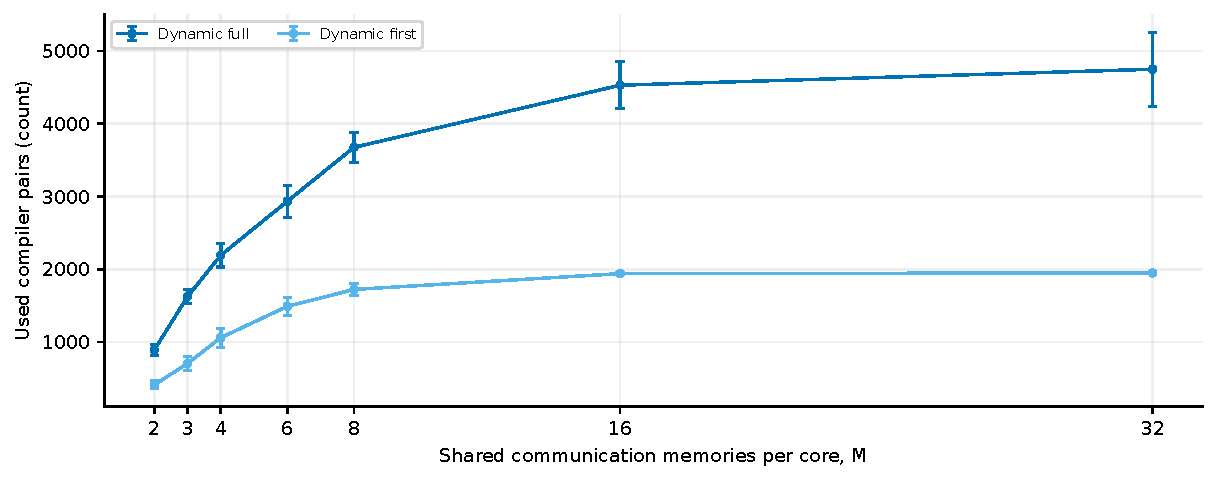
\includegraphics[width=.94\linewidth,height=.255\textheight,keepaspectratio]{figures/memory/mesh_max_reliability_utilized_compiler_pairs.pdf}\captionof{figure}{Run-level mean and sample SD. Shared trace aliases are counted once.}\end{center}
\begin{center}{\scriptsize\setlength{\tabcolsep}{3pt}
\begin{tabular}{lrrrrr}
\toprule
M & ODG & CGP & ACGP & Dynamic full & Dynamic first \\
\midrule
2 & n/a & n/a & n/a & $888.00\pm70.82$ & $410.00\pm53.53$ \\
3 & n/a & n/a & n/a & $1623.00\pm99.87$ & $703.33\pm99.35$ \\
4 & n/a & n/a & n/a & $2191.83\pm161.34$ & $1058.83\pm132.19$ \\
6 & n/a & n/a & n/a & $2934.50\pm219.96$ & $1489.00\pm120.01$ \\
8 & n/a & n/a & n/a & $3675.00\pm206.88$ & $1721.67\pm86.80$ \\
16 & n/a & n/a & n/a & $4529.83\pm321.49$ & $1939.33\pm15.83$ \\
32 & n/a & n/a & n/a & $4749.50\pm507.48$ & $1949.00\pm3.74$ \\
\bottomrule\end{tabular}}
\captionof{table}{Mean $\pm$ sample SD; n/a denotes a metric outside that policy's instrumentation.}
{\footnotesize\href{https://github.com/sanjeevkrishnaa/Compiler-Driven-ACE/blob/codex/ace-scheduler-correctness/docs/latex/qft96_final/data/memory_mesh_max_reliability_utilized_compiler_pairs.csv}{Exact CSV values and sample counts}}
\end{center}
\clearpage
\subsection*{Expired compiler pairs}
\begin{center}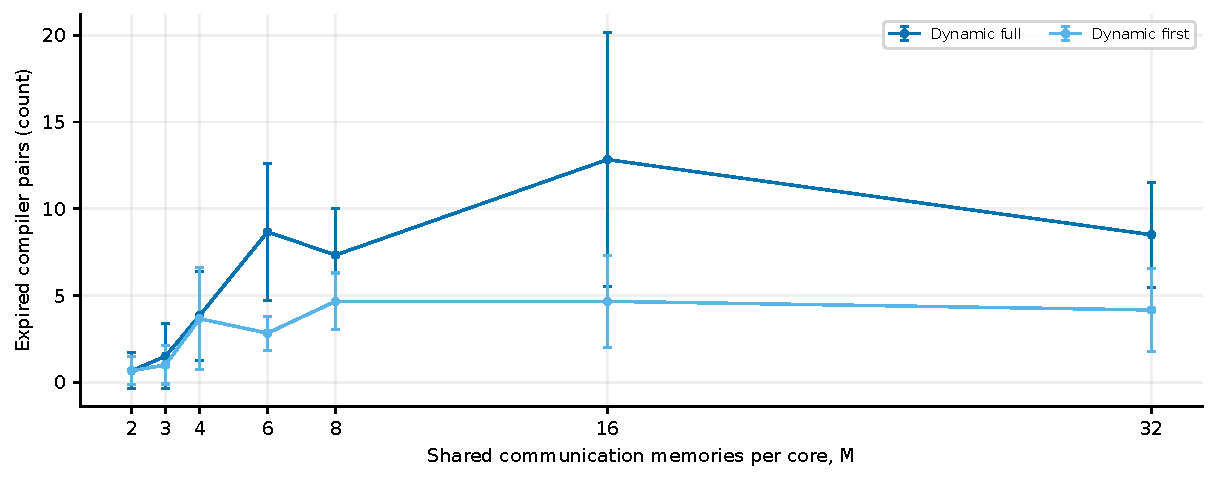
\includegraphics[width=.94\linewidth,height=.255\textheight,keepaspectratio]{figures/memory/mesh_max_reliability_expired_compiler_pairs.pdf}\captionof{figure}{Run-level mean and sample SD. Shared trace aliases are counted once.}\end{center}
\begin{center}{\scriptsize\setlength{\tabcolsep}{3pt}
\begin{tabular}{lrrrrr}
\toprule
M & ODG & CGP & ACGP & Dynamic full & Dynamic first \\
\midrule
2 & n/a & n/a & n/a & $0.6667\pm1.0328$ & $0.6667\pm0.8165$ \\
3 & n/a & n/a & n/a & $1.500\pm1.871$ & $1.000\pm1.095$ \\
4 & n/a & n/a & n/a & $3.833\pm2.563$ & $3.667\pm2.944$ \\
6 & n/a & n/a & n/a & $8.667\pm3.933$ & $2.833\pm0.983$ \\
8 & n/a & n/a & n/a & $7.333\pm2.658$ & $4.667\pm1.633$ \\
16 & n/a & n/a & n/a & $12.833\pm7.333$ & $4.667\pm2.658$ \\
32 & n/a & n/a & n/a & $8.500\pm3.017$ & $4.167\pm2.401$ \\
\bottomrule\end{tabular}}
\captionof{table}{Mean $\pm$ sample SD; n/a denotes a metric outside that policy's instrumentation.}
{\footnotesize\href{https://github.com/sanjeevkrishnaa/Compiler-Driven-ACE/blob/codex/ace-scheduler-correctness/docs/latex/qft96_final/data/memory_mesh_max_reliability_expired_compiler_pairs.csv}{Exact CSV values and sample counts}}
\end{center}
\subsection*{Remaining compiler pairs}
\begin{center}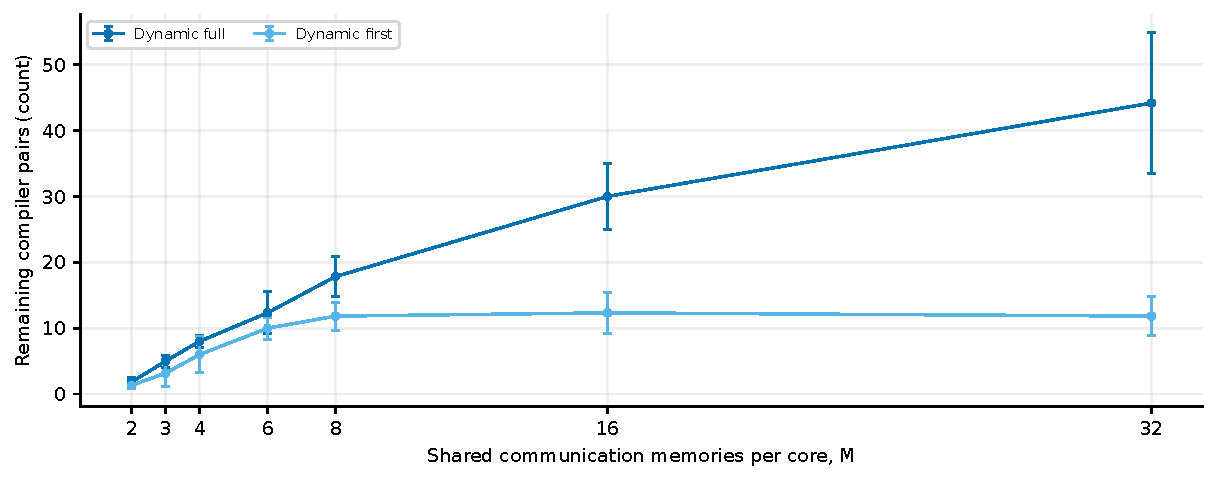
\includegraphics[width=.94\linewidth,height=.255\textheight,keepaspectratio]{figures/memory/mesh_max_reliability_remaining_compiler_pairs.pdf}\captionof{figure}{Run-level mean and sample SD. Shared trace aliases are counted once.}\end{center}
\begin{center}{\scriptsize\setlength{\tabcolsep}{3pt}
\begin{tabular}{lrrrrr}
\toprule
M & ODG & CGP & ACGP & Dynamic full & Dynamic first \\
\midrule
2 & n/a & n/a & n/a & $1.833\pm0.753$ & $1.333\pm0.516$ \\
3 & n/a & n/a & n/a & $5.000\pm0.894$ & $3.167\pm1.941$ \\
4 & n/a & n/a & n/a & $8.000\pm0.894$ & $6.000\pm2.757$ \\
6 & n/a & n/a & n/a & $12.333\pm3.204$ & $10.000\pm1.673$ \\
8 & n/a & n/a & n/a & $17.833\pm3.061$ & $11.833\pm2.137$ \\
16 & n/a & n/a & n/a & $30.000\pm4.980$ & $12.333\pm3.077$ \\
32 & n/a & n/a & n/a & $44.167\pm10.722$ & $11.833\pm2.927$ \\
\bottomrule\end{tabular}}
\captionof{table}{Mean $\pm$ sample SD; n/a denotes a metric outside that policy's instrumentation.}
{\footnotesize\href{https://github.com/sanjeevkrishnaa/Compiler-Driven-ACE/blob/codex/ace-scheduler-correctness/docs/latex/qft96_final/data/memory_mesh_max_reliability_remaining_compiler_pairs.csv}{Exact CSV values and sample counts}}
\end{center}
\clearpage
\subsection*{Compiler fidelity at creation}
\begin{center}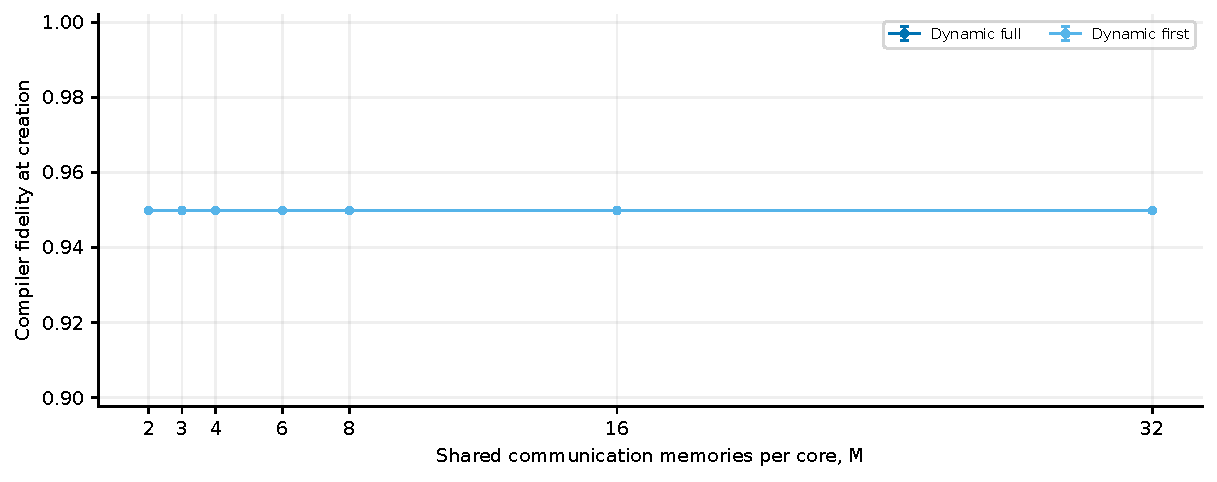
\includegraphics[width=.94\linewidth,height=.255\textheight,keepaspectratio]{figures/memory/mesh_max_reliability_average_fidelity_at_creation.pdf}\captionof{figure}{Run-level mean and sample SD. Shared trace aliases are counted once.}\end{center}
\begin{center}{\scriptsize\setlength{\tabcolsep}{3pt}
\begin{tabular}{lrrrrr}
\toprule
M & ODG & CGP & ACGP & Dynamic full & Dynamic first \\
\midrule
2 & n/a & n/a & n/a & $0.9498\pm0.0000$ & $0.9498\pm0.0000$ \\
3 & n/a & n/a & n/a & $0.9498\pm0.0000$ & $0.9498\pm0.0000$ \\
4 & n/a & n/a & n/a & $0.9498\pm0.0000$ & $0.9498\pm0.0000$ \\
6 & n/a & n/a & n/a & $0.9498\pm0.0000$ & $0.9498\pm0.0000$ \\
8 & n/a & n/a & n/a & $0.9498\pm0.0000$ & $0.9498\pm0.0000$ \\
16 & n/a & n/a & n/a & $0.9498\pm0.0000$ & $0.9498\pm0.0000$ \\
32 & n/a & n/a & n/a & $0.9498\pm0.0000$ & $0.9498\pm0.0000$ \\
\bottomrule\end{tabular}}
\captionof{table}{Mean $\pm$ sample SD; n/a denotes a metric outside that policy's instrumentation.}
{\footnotesize\href{https://github.com/sanjeevkrishnaa/Compiler-Driven-ACE/blob/codex/ace-scheduler-correctness/docs/latex/qft96_final/data/memory_mesh_max_reliability_average_fidelity_at_creation.csv}{Exact CSV values and sample counts}}
\end{center}
\subsection*{Compiler fidelity at use}
\begin{center}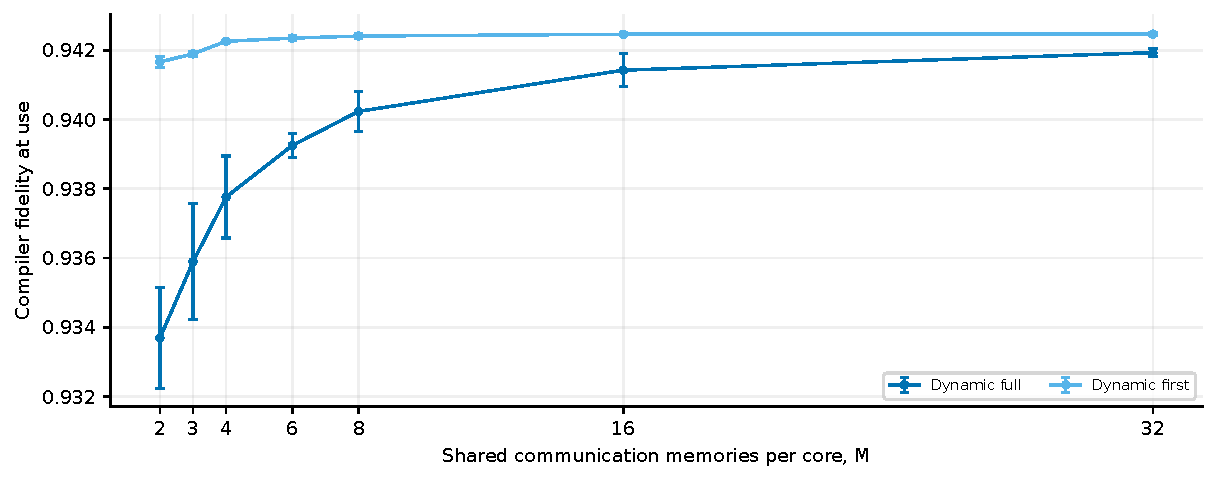
\includegraphics[width=.94\linewidth,height=.255\textheight,keepaspectratio]{figures/memory/mesh_max_reliability_average_fidelity_at_utilization.pdf}\captionof{figure}{Run-level mean and sample SD. Shared trace aliases are counted once.}\end{center}
\begin{center}{\scriptsize\setlength{\tabcolsep}{3pt}
\begin{tabular}{lrrrrr}
\toprule
M & ODG & CGP & ACGP & Dynamic full & Dynamic first \\
\midrule
2 & n/a & n/a & n/a & $0.9337\pm0.0015$ & $0.9417\pm0.0002$ \\
3 & n/a & n/a & n/a & $0.9359\pm0.0017$ & $0.9419\pm0.0001$ \\
4 & n/a & n/a & n/a & $0.9378\pm0.0012$ & $0.9423\pm0.0000$ \\
6 & n/a & n/a & n/a & $0.9393\pm0.0003$ & $0.9424\pm0.0001$ \\
8 & n/a & n/a & n/a & $0.9402\pm0.0006$ & $0.9424\pm0.0001$ \\
16 & n/a & n/a & n/a & $0.9414\pm0.0005$ & $0.9425\pm0.0000$ \\
32 & n/a & n/a & n/a & $0.9419\pm0.0001$ & $0.9425\pm0.0001$ \\
\bottomrule\end{tabular}}
\captionof{table}{Mean $\pm$ sample SD; n/a denotes a metric outside that policy's instrumentation.}
{\footnotesize\href{https://github.com/sanjeevkrishnaa/Compiler-Driven-ACE/blob/codex/ace-scheduler-correctness/docs/latex/qft96_final/data/memory_mesh_max_reliability_average_fidelity_at_utilization.csv}{Exact CSV values and sample counts}}
\end{center}
\clearpage
\subsection*{Mean layer latency}
\begin{center}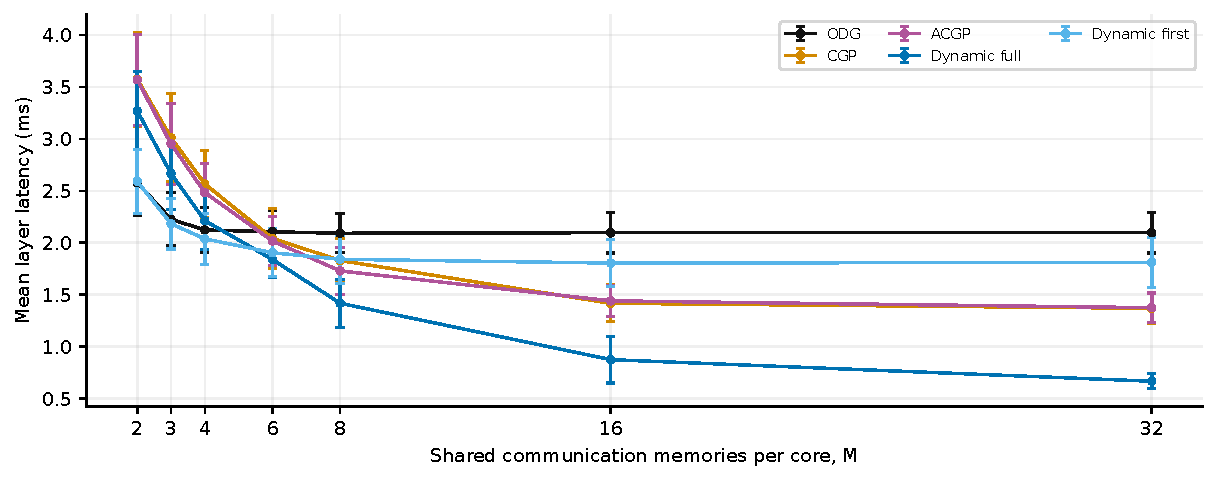
\includegraphics[width=.94\linewidth,height=.255\textheight,keepaspectratio]{figures/memory/mesh_max_reliability_avg_layer_latency_ms.pdf}\captionof{figure}{Run-level mean and sample SD. Shared trace aliases are counted once.}\end{center}
\begin{center}{\scriptsize\setlength{\tabcolsep}{3pt}
\begin{tabular}{lrrrrr}
\toprule
M & ODG & CGP & ACGP & Dynamic full & Dynamic first \\
\midrule
2 & $2.578\pm0.318$ & $3.575\pm0.451$ & $3.570\pm0.439$ & $3.271\pm0.376$ & $2.593\pm0.309$ \\
3 & $2.227\pm0.255$ & $3.012\pm0.422$ & $2.952\pm0.393$ & $2.666\pm0.347$ & $2.183\pm0.243$ \\
4 & $2.123\pm0.213$ & $2.566\pm0.318$ & $2.484\pm0.279$ & $2.213\pm0.279$ & $2.038\pm0.246$ \\
6 & $2.106\pm0.204$ & $2.043\pm0.288$ & $2.017\pm0.238$ & $1.839\pm0.172$ & $1.904\pm0.231$ \\
8 & $2.092\pm0.188$ & $1.829\pm0.215$ & $1.730\pm0.227$ & $1.418\pm0.232$ & $1.842\pm0.229$ \\
16 & $2.098\pm0.196$ & $1.418\pm0.176$ & $1.441\pm0.152$ & $0.8752\pm0.2248$ & $1.805\pm0.228$ \\
32 & $2.098\pm0.196$ & $1.369\pm0.149$ & $1.375\pm0.142$ & $0.6673\pm0.0722$ & $1.812\pm0.238$ \\
\bottomrule\end{tabular}}
\captionof{table}{Mean $\pm$ sample SD; n/a denotes a metric outside that policy's instrumentation.}
{\footnotesize\href{https://github.com/sanjeevkrishnaa/Compiler-Driven-ACE/blob/codex/ace-scheduler-correctness/docs/latex/qft96_final/data/memory_mesh_max_reliability_avg_layer_latency_ms.csv}{Exact CSV values and sample counts}}
\end{center}
\subsection*{Maximum layer latency}
\begin{center}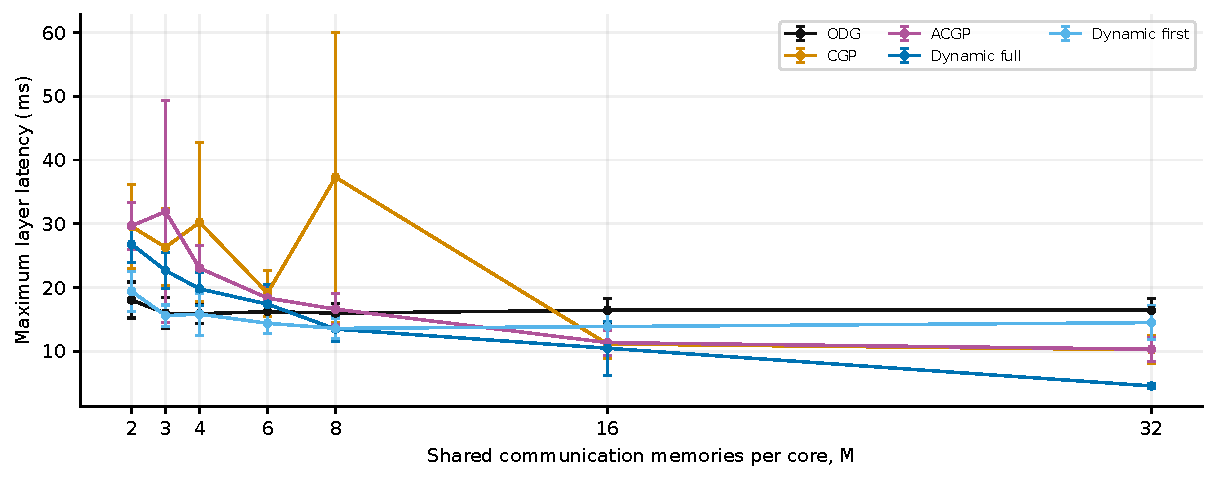
\includegraphics[width=.94\linewidth,height=.255\textheight,keepaspectratio]{figures/memory/mesh_max_reliability_max_layer_latency_ms.pdf}\captionof{figure}{Run-level mean and sample SD. Shared trace aliases are counted once.}\end{center}
\begin{center}{\scriptsize\setlength{\tabcolsep}{3pt}
\begin{tabular}{lrrrrr}
\toprule
M & ODG & CGP & ACGP & Dynamic full & Dynamic first \\
\midrule
2 & $18.034\pm2.826$ & $29.567\pm6.586$ & $29.667\pm3.669$ & $26.784\pm2.811$ & $19.417\pm3.142$ \\
3 & $15.950\pm2.414$ & $26.301\pm6.023$ & $31.895\pm17.457$ & $22.667\pm2.853$ & $15.584\pm1.665$ \\
4 & $15.884\pm1.548$ & $30.222\pm12.448$ & $23.034\pm3.606$ & $19.784\pm2.604$ & $15.817\pm3.316$ \\
6 & $16.200\pm1.842$ & $19.117\pm3.601$ & $18.338\pm1.888$ & $17.384\pm3.077$ & $14.384\pm1.618$ \\
8 & $15.984\pm1.491$ & $37.292\pm22.728$ & $16.600\pm2.436$ & $13.467\pm1.984$ & $13.584\pm1.517$ \\
16 & $16.434\pm1.876$ & $11.133\pm2.296$ & $11.349\pm1.960$ & $10.467\pm4.229$ & $13.867\pm2.381$ \\
32 & $16.434\pm1.876$ & $10.223\pm2.170$ & $10.317\pm1.891$ & $4.550\pm0.437$ & $14.484\pm2.666$ \\
\bottomrule\end{tabular}}
\captionof{table}{Mean $\pm$ sample SD; n/a denotes a metric outside that policy's instrumentation.}
{\footnotesize\href{https://github.com/sanjeevkrishnaa/Compiler-Driven-ACE/blob/codex/ace-scheduler-correctness/docs/latex/qft96_final/data/memory_mesh_max_reliability_max_layer_latency_ms.csv}{Exact CSV values and sample counts}}
\end{center}
\clearpage
\subsection*{Minimum layer latency}
\begin{center}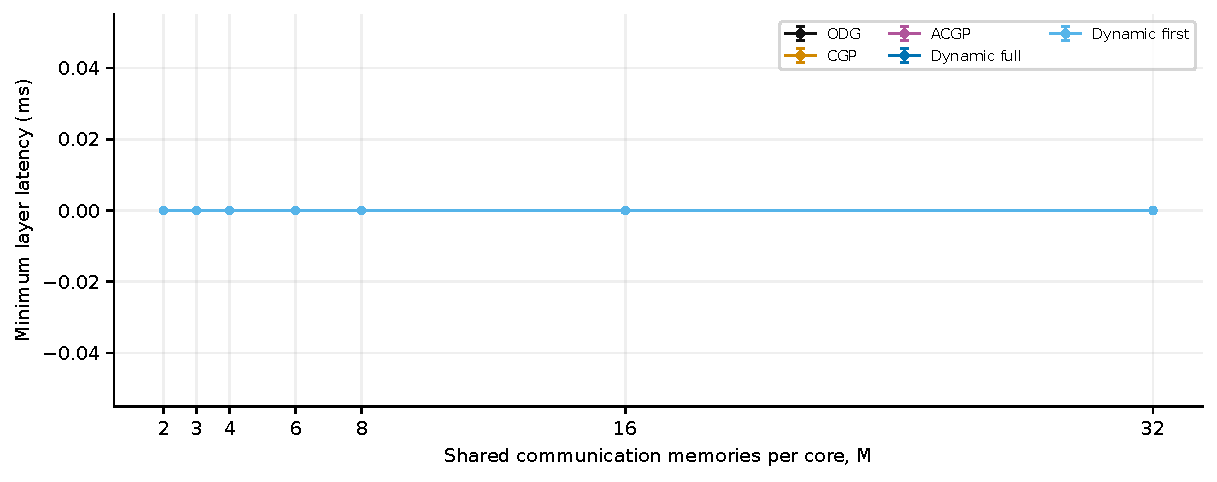
\includegraphics[width=.94\linewidth,height=.255\textheight,keepaspectratio]{figures/memory/mesh_max_reliability_min_layer_latency_ms.pdf}\captionof{figure}{Run-level mean and sample SD. Shared trace aliases are counted once.}\end{center}
\begin{center}{\scriptsize\setlength{\tabcolsep}{3pt}
\begin{tabular}{lrrrrr}
\toprule
M & ODG & CGP & ACGP & Dynamic full & Dynamic first \\
\midrule
2 & $0.0000\pm0.0000$ & $0.0000\pm0.0000$ & $0.0000\pm0.0000$ & $0.0000\pm0.0000$ & $0.0000\pm0.0000$ \\
3 & $0.0000\pm0.0000$ & $0.0000\pm0.0000$ & $0.0000\pm0.0000$ & $0.0000\pm0.0000$ & $0.0000\pm0.0000$ \\
4 & $0.0000\pm0.0000$ & $0.0000\pm0.0000$ & $0.0000\pm0.0000$ & $0.0000\pm0.0000$ & $0.0000\pm0.0000$ \\
6 & $0.0000\pm0.0000$ & $0.0000\pm0.0000$ & $0.0000\pm0.0000$ & $0.0000\pm0.0000$ & $0.0000\pm0.0000$ \\
8 & $0.0000\pm0.0000$ & $0.0000\pm0.0000$ & $0.0000\pm0.0000$ & $0.0000\pm0.0000$ & $0.0000\pm0.0000$ \\
16 & $0.0000\pm0.0000$ & $0.0000\pm0.0000$ & $0.0000\pm0.0000$ & $0.0000\pm0.0000$ & $0.0000\pm0.0000$ \\
32 & $0.0000\pm0.0000$ & $0.0000\pm0.0000$ & $0.0000\pm0.0000$ & $0.0000\pm0.0000$ & $0.0000\pm0.0000$ \\
\bottomrule\end{tabular}}
\captionof{table}{Mean $\pm$ sample SD; n/a denotes a metric outside that policy's instrumentation.}
{\footnotesize\href{https://github.com/sanjeevkrishnaa/Compiler-Driven-ACE/blob/codex/ace-scheduler-correctness/docs/latex/qft96_final/data/memory_mesh_max_reliability_min_layer_latency_ms.csv}{Exact CSV values and sample counts}}
\end{center}